\documentclass{article}

% use numbers for citations to save space
\PassOptionsToPackage{numbers, compress}{natbib}

% either empty (for submission), 'preprint', or 'final'
\def\status{preprint}
\usepackage[\status]{neurips_2024}

% TOC for document parts, must be included before hyperref!
% (https://latex.org/forum/viewtopic.php?t=2014)
\usepackage{titletoc}
%%% Local Variables:
%%% mode: latex
%%% TeX-master: "../main"
%%% End:

\usepackage[utf8]{inputenc} % allow utf-8 input
\usepackage[T1]{fontenc}    % use 8-bit T1 fonts
\usepackage{hyperref}       % hyperlinks
\usepackage{url}            % simple URL typesetting
\usepackage{booktabs}       % professional-quality tables
\usepackage{amsfonts}       % blackboard math symbols
\usepackage{nicefrac}       % compact symbols for 1/2, etc.
\usepackage{microtype}      % microtypography
\usepackage{xcolor}         % colors
%%% Local Variables:
%%% mode: latex
%%% TeX-master: "../main"
%%% End:

% follow DL notation from the Goodfellow book
% requirements
\usepackage{amsmath}
\usepackage{amssymb}
\usepackage{bm}
\usepackage{mathtools}

% Random variables
\def\reta{{\textnormal{$\eta$}}}
\def\ra{{\textnormal{a}}}
\def\rb{{\textnormal{b}}}
\def\rc{{\textnormal{c}}}
\def\rd{{\textnormal{d}}}
\def\re{{\textnormal{e}}}
\def\rf{{\textnormal{f}}}
\def\rg{{\textnormal{g}}}
\def\rh{{\textnormal{h}}}
\def\ri{{\textnormal{i}}}
\def\rj{{\textnormal{j}}}
\def\rk{{\textnormal{k}}}
\def\rl{{\textnormal{l}}}
% rm is already a command, just don't name any random variables m
\def\rn{{\textnormal{n}}}
\def\ro{{\textnormal{o}}}
\def\rp{{\textnormal{p}}}
\def\rq{{\textnormal{q}}}
\def\rr{{\textnormal{r}}}
\def\rs{{\textnormal{s}}}
\def\rt{{\textnormal{t}}}
\def\ru{{\textnormal{u}}}
\def\rv{{\textnormal{v}}}
\def\rw{{\textnormal{w}}}
\def\rx{{\textnormal{x}}}
\def\ry{{\textnormal{y}}}
\def\rz{{\textnormal{z}}}

% Random vectors
\def\rvepsilon{{\mathbf{\epsilon}}}
\def\rvtheta{{\mathbf{\theta}}}
\def\rva{{\mathbf{a}}}
\def\rvb{{\mathbf{b}}}
\def\rvc{{\mathbf{c}}}
\def\rvd{{\mathbf{d}}}
\def\rve{{\mathbf{e}}}
\def\rvf{{\mathbf{f}}}
\def\rvg{{\mathbf{g}}}
\def\rvh{{\mathbf{h}}}
\def\rvu{{\mathbf{i}}}
\def\rvj{{\mathbf{j}}}
\def\rvk{{\mathbf{k}}}
\def\rvl{{\mathbf{l}}}
\def\rvm{{\mathbf{m}}}
\def\rvn{{\mathbf{n}}}
\def\rvo{{\mathbf{o}}}
\def\rvp{{\mathbf{p}}}
\def\rvq{{\mathbf{q}}}
\def\rvr{{\mathbf{r}}}
\def\rvs{{\mathbf{s}}}
\def\rvt{{\mathbf{t}}}
\def\rvu{{\mathbf{u}}}
\def\rvv{{\mathbf{v}}}
\def\rvw{{\mathbf{w}}}
\def\rvx{{\mathbf{x}}}
\def\rvy{{\mathbf{y}}}
\def\rvz{{\mathbf{z}}}

% Elements of random vectors
\def\erva{{\textnormal{a}}}
\def\ervb{{\textnormal{b}}}
\def\ervc{{\textnormal{c}}}
\def\ervd{{\textnormal{d}}}
\def\erve{{\textnormal{e}}}
\def\ervf{{\textnormal{f}}}
\def\ervg{{\textnormal{g}}}
\def\ervh{{\textnormal{h}}}
\def\ervi{{\textnormal{i}}}
\def\ervj{{\textnormal{j}}}
\def\ervk{{\textnormal{k}}}
\def\ervl{{\textnormal{l}}}
\def\ervm{{\textnormal{m}}}
\def\ervn{{\textnormal{n}}}
\def\ervo{{\textnormal{o}}}
\def\ervp{{\textnormal{p}}}
\def\ervq{{\textnormal{q}}}
\def\ervr{{\textnormal{r}}}
\def\ervs{{\textnormal{s}}}
\def\ervt{{\textnormal{t}}}
\def\ervu{{\textnormal{u}}}
\def\ervv{{\textnormal{v}}}
\def\ervw{{\textnormal{w}}}
\def\ervx{{\textnormal{x}}}
\def\ervy{{\textnormal{y}}}
\def\ervz{{\textnormal{z}}}

% Random matrices
\def\rmA{{\mathbf{A}}}
\def\rmB{{\mathbf{B}}}
\def\rmC{{\mathbf{C}}}
\def\rmD{{\mathbf{D}}}
\def\rmE{{\mathbf{E}}}
\def\rmF{{\mathbf{F}}}
\def\rmG{{\mathbf{G}}}
\def\rmH{{\mathbf{H}}}
\def\rmI{{\mathbf{I}}}
\def\rmJ{{\mathbf{J}}}
\def\rmK{{\mathbf{K}}}
\def\rmL{{\mathbf{L}}}
\def\rmM{{\mathbf{M}}}
\def\rmN{{\mathbf{N}}}
\def\rmO{{\mathbf{O}}}
\def\rmP{{\mathbf{P}}}
\def\rmQ{{\mathbf{Q}}}
\def\rmR{{\mathbf{R}}}
\def\rmS{{\mathbf{S}}}
\def\rmT{{\mathbf{T}}}
\def\rmU{{\mathbf{U}}}
\def\rmV{{\mathbf{V}}}
\def\rmW{{\mathbf{W}}}
\def\rmX{{\mathbf{X}}}
\def\rmY{{\mathbf{Y}}}
\def\rmZ{{\mathbf{Z}}}

% Elements of random matrices
\def\ermA{{\textnormal{A}}}
\def\ermB{{\textnormal{B}}}
\def\ermC{{\textnormal{C}}}
\def\ermD{{\textnormal{D}}}
\def\ermE{{\textnormal{E}}}
\def\ermF{{\textnormal{F}}}
\def\ermG{{\textnormal{G}}}
\def\ermH{{\textnormal{H}}}
\def\ermI{{\textnormal{I}}}
\def\ermJ{{\textnormal{J}}}
\def\ermK{{\textnormal{K}}}
\def\ermL{{\textnormal{L}}}
\def\ermM{{\textnormal{M}}}
\def\ermN{{\textnormal{N}}}
\def\ermO{{\textnormal{O}}}
\def\ermP{{\textnormal{P}}}
\def\ermQ{{\textnormal{Q}}}
\def\ermR{{\textnormal{R}}}
\def\ermS{{\textnormal{S}}}
\def\ermT{{\textnormal{T}}}
\def\ermU{{\textnormal{U}}}
\def\ermV{{\textnormal{V}}}
\def\ermW{{\textnormal{W}}}
\def\ermX{{\textnormal{X}}}
\def\ermY{{\textnormal{Y}}}
\def\ermZ{{\textnormal{Z}}}

% Vectors
\def\vzero{{\bm{0}}}
\def\vone{{\bm{1}}}
\def\vmu{{\bm{\mu}}}
\def\vnu{{\bm{\nu}}}
\def\vtheta{{\bm{\theta}}}
\def\vepsilon{{\bm{\epsilon}}}
\def\vgamma{{\bm{\gamma}}}
\def\vdelta{{\bm{\delta}}}
\def\vDelta{{\bm{\Delta}}}
\def\va{{\bm{a}}}
\def\vb{{\bm{b}}}
\def\vc{{\bm{c}}}
\def\vd{{\bm{d}}}
\def\ve{{\bm{e}}}
\def\vetilde{\bm{\tilde{e}}}
\def\vell{{\bm{\ell}}}
\def\vf{{\bm{f}}}
\def\vg{{\bm{g}}}
\def\vh{{\bm{h}}}
\def\vi{{\bm{i}}}
\def\vj{{\bm{j}}}
\def\vk{{\bm{k}}}
\def\vl{{\bm{l}}}
\def\vm{{\bm{m}}}
\def\vmhat{{\bm{\hat{m}}}}
\def\vn{{\bm{n}}}
\def\vo{{\bm{o}}}
\def\vp{{\bm{p}}}
\def\vphi{{\bm{\phi}}}
\def\vq{{\bm{q}}}
\def\vr{{\bm{r}}}
\def\vs{{\bm{s}}}
\def\vstilde{\bm{\tilde{s}}}
\def\vt{{\bm{t}}}
\def\vu{{\bm{u}}}
\def\vv{{\bm{v}}}
\def\vvhat{{\bm{\hat{v}}}}
\def\vw{{\bm{w}}}
\def\vx{{\bm{x}}}
\def\vy{{\bm{y}}}
\def\vytilde{{\bm{\tilde{y}}}}
\def\vyhat{{\bm{\hat{y}}}}
\def\vz{{\bm{z}}}

% Elements of vectors
\def\evalpha{{\alpha}}
\def\evbeta{{\beta}}
\def\evepsilon{{\epsilon}}
\def\evlambda{{\lambda}}
\def\evomega{{\omega}}
\def\evmu{{\mu}}
\def\evpsi{{\psi}}
\def\evsigma{{\sigma}}
\def\evtheta{{\theta}}
\def\eva{{a}}
\def\evb{{b}}
\def\evc{{c}}
\def\evd{{d}}
\def\eve{{e}}
\def\evf{{f}}
\def\evg{{g}}
\def\evh{{h}}
\def\evi{{i}}
\def\evj{{j}}
\def\evk{{k}}
\def\evl{{l}}
\def\evm{{m}}
\def\evn{{n}}
\def\evo{{o}}
\def\evp{{p}}
\def\evq{{q}}
\def\evr{{r}}
\def\evs{{s}}
\def\evt{{t}}
\def\evu{{u}}
\def\evv{{v}}
\def\evw{{w}}
\def\evx{{x}}
\def\evy{{y}}
\def\evyhat{{\hat{y}}}
\def\evz{{z}}

% Matrix
\def\mA{{\bm{A}}}
\def\mB{{\bm{B}}}
\def\mC{{\bm{C}}}
\def\mD{{\bm{D}}}
\def\mE{{\bm{E}}}
\def\mF{{\bm{F}}}
\def\mG{{\bm{G}}}
\def\mGtilde{\bm{\tilde{G}}}
\def\mH{{\bm{H}}}
\def\mI{{\bm{I}}}
\def\mJ{{\bm{J}}}
\def\mK{{\bm{K}}}
\def\mL{{\bm{L}}}
\def\mM{{\bm{M}}}
\def\mN{{\bm{N}}}
\def\mO{{\bm{O}}}
\def\mP{{\bm{P}}}
\def\mQ{{\bm{Q}}}
\def\mR{{\bm{R}}}
\def\mS{{\bm{S}}}
\def\mT{{\bm{T}}}
\def\mU{{\bm{U}}}
\def\mV{{\bm{V}}}
\def\mW{{\bm{W}}}
\def\mX{{\bm{X}}}
\def\mY{{\bm{Y}}}
\def\mZ{{\bm{Z}}}
\def\mBeta{{\bm{\beta}}}
\def\mGamma{{\bm{\Gamma}}}
\def\mPhi{{\bm{\Phi}}}
\def\mPi{{\bm{\Pi}}}
\def\mLambda{{\bm{\Lambda}}}
\def\mSigma{{\bm{\Sigma}}}
\def\mOmega{{\bm{\Omega}}}
\def\mStilde{\bm{\tilde{\mS}}}
\def\mGtilde{\bm{\tilde{\mG}}}
\def\mGoverline{{\bm{\overline{G}}}}

% Tensor
\DeclareMathAlphabet{\mathsfit}{\encodingdefault}{\sfdefault}{m}{sl}
\SetMathAlphabet{\mathsfit}{bold}{\encodingdefault}{\sfdefault}{bx}{n}
\newcommand{\tens}[1]{\bm{\mathsfit{#1}}}
\def\tA{{\tens{A}}}
\def\tB{{\tens{B}}}
\def\tC{{\tens{C}}}
\def\tD{{\tens{D}}}
\def\tE{{\tens{E}}}
\def\tF{{\tens{F}}}
\def\tG{{\tens{G}}}
\def\tH{{\tens{H}}}
\def\tI{{\tens{I}}}
\def\tJ{{\tens{J}}}
\def\tK{{\tens{K}}}
\def\tL{{\tens{L}}}
\def\tM{{\tens{M}}}
\def\tN{{\tens{N}}}
\def\tO{{\tens{O}}}
\def\tP{{\tens{P}}}
\def\tPi{\bm{\mathsf{\Pi}}}
\def\tQ{{\tens{Q}}}
\def\tR{{\tens{R}}}
\def\tS{{\tens{S}}}
\def\tT{{\tens{T}}}
\def\tU{{\tens{U}}}
\def\tV{{\tens{V}}}
\def\tW{{\tens{W}}}
\def\tX{{\tens{X}}}
\def\tY{{\tens{Y}}}
\def\tZ{{\tens{Z}}}

% Graph
\def\gA{{\mathcal{A}}}
\def\gB{{\mathcal{B}}}
\def\gC{{\mathcal{C}}}
\def\gD{{\mathcal{D}}}
\def\gE{{\mathcal{E}}}
\def\gF{{\mathcal{F}}}
\def\gG{{\mathcal{G}}}
\def\gH{{\mathcal{H}}}
\def\gI{{\mathcal{I}}}
\def\gJ{{\mathcal{J}}}
\def\gK{{\mathcal{K}}}
\def\gL{{\mathcal{L}}}
\def\gM{{\mathcal{M}}}
\def\gN{{\mathcal{N}}}
\def\gO{{\mathcal{O}}}
\def\gP{{\mathcal{P}}}
\def\gQ{{\mathcal{Q}}}
\def\gR{{\mathcal{R}}}
\def\gS{{\mathcal{S}}}
\def\gT{{\mathcal{T}}}
\def\gU{{\mathcal{U}}}
\def\gV{{\mathcal{V}}}
\def\gW{{\mathcal{W}}}
\def\gX{{\mathcal{X}}}
\def\gY{{\mathcal{Y}}}
\def\gZ{{\mathcal{Z}}}

% Sets
\def\sA{{\mathbb{A}}}
\def\sB{{\mathbb{B}}}
\def\sC{{\mathbb{C}}}
\def\sD{{\mathbb{D}}}
% Don't use a set called E, because this would be the same as our symbol
% for expectation.
\def\sF{{\mathbb{F}}}
\def\sG{{\mathbb{G}}}
\def\sH{{\mathbb{H}}}
\def\sI{{\mathbb{I}}}
\def\sJ{{\mathbb{J}}}
\def\sK{{\mathbb{K}}}
\def\sL{{\mathbb{L}}}
\def\sM{{\mathbb{M}}}
\def\sN{{\mathbb{N}}}
\def\sO{{\mathbb{O}}}
\def\sP{{\mathbb{P}}}
\def\sQ{{\mathbb{Q}}}
\def\sR{{\mathbb{R}}}
\def\sS{{\mathbb{S}}}
\def\sT{{\mathbb{T}}}
\def\sU{{\mathbb{U}}}
\def\sV{{\mathbb{V}}}
\def\sW{{\mathbb{W}}}
\def\sX{{\mathbb{X}}}
\def\sY{{\mathbb{Y}}}
\def\sYhat{{\hat{\mathbb{Y}}}}
\def\sZ{{\mathbb{Z}}}
% Blackboard Greek characters: https://tex.stackexchange.com/a/3260
\DeclareSymbolFont{bbold}{U}{bbold}{m}{n}
\DeclareSymbolFontAlphabet{\mathbbold}{bbold}
\def\sTheta{{\mathbbold{\Theta}}}
\def\sOmega{{\mathbbold{\Omega}}}

% Entries of a matrix
\def\emLambda{{\Lambda}}
\def\emA{{A}}
\def\emB{{B}}
\def\emC{{C}}
\def\emD{{D}}
\def\emE{{E}}
\def\emF{{F}}
\def\emG{{G}}
\def\emH{{H}}
\def\emI{{I}}
\def\emJ{{J}}
\def\emK{{K}}
\def\emL{{L}}
\def\emM{{M}}
\def\emN{{N}}
\def\emO{{O}}
\def\emP{{P}}
\def\emQ{{Q}}
\def\emR{{R}}
\def\emS{{S}}
\def\emT{{T}}
\def\emU{{U}}
\def\emV{{V}}
\def\emW{{W}}
\def\emX{{X}}
\def\emY{{Y}}
\def\emZ{{Z}}
\def\emSigma{{\Sigma}}
\def\emPi{{\Pi}}

% entries of a tensor
% Same font as tensor, without \bm wrapper
\newcommand{\etens}[1]{\mathsfit{#1}}
\def\etLambda{{\etens{\Lambda}}}
\def\etA{{\etens{A}}}
\def\etB{{\etens{B}}}
\def\etC{{\etens{C}}}
\def\etD{{\etens{D}}}
\def\etE{{\etens{E}}}
\def\etF{{\etens{F}}}
\def\etG{{\etens{G}}}
\def\etH{{\etens{H}}}
\def\etI{{\etens{I}}}
\def\etJ{{\etens{J}}}
\def\etK{{\etens{K}}}
\def\etL{{\etens{L}}}
\def\etM{{\etens{M}}}
\def\etN{{\etens{N}}}
\def\etO{{\etens{O}}}
\def\etP{{\etens{P}}}
\def\etPi{\mathsf{\Pi}}
\def\etQ{{\etens{Q}}}
\def\etR{{\etens{R}}}
\def\etS{{\etens{S}}}
\def\etT{{\etens{T}}}
\def\etU{{\etens{U}}}
\def\etV{{\etens{V}}}
\def\etW{{\etens{W}}}
\def\etX{{\etens{X}}}
\def\etY{{\etens{Y}}}
\def\etZ{{\etens{Z}}}

% The true underlying data generating distribution
\newcommand{\pdata}{p_{\mathrm{data}}}
% The empirical distribution defined by the training set
\newcommand{\ptrain}{\hat{p}_{\mathrm{data}}}
\newcommand{\Ptrain}{\hat{P}_{\mathrm{data}}}
% The model distribution
\newcommand{\pmodel}{p_{\rm{model}}}
\newcommand{\Pmodel}{P_{\rm{model}}}
\newcommand{\ptildemodel}{\tilde{p}_{\rm{model}}}
% Stochastic autoencoder distributions
\newcommand{\pencode}{p_{\rm{encoder}}}
\newcommand{\pdecode}{p_{\rm{decoder}}}
\newcommand{\precons}{p_{\rm{reconstruct}}}

\newcommand{\laplace}{\mathrm{Laplace}} % Laplace distribution

\newcommand{\E}{\mathbb{E}}
\newcommand{\Ls}{\mathcal{L}}
\newcommand{\R}{\mathbb{R}}
\newcommand{\emp}{\tilde{p}}
\newcommand{\lr}{\alpha}
\newcommand{\reg}{\lambda}
\newcommand{\rect}{\mathrm{rectifier}}
\newcommand{\softmax}{\mathrm{softmax}}
\newcommand{\onehot}{\mathrm{onehot}}
\newcommand{\sigmoid}{\sigma}
\newcommand{\softplus}{\zeta}
\newcommand{\KL}{D_{\mathrm{KL}}}
\newcommand{\Var}{\mathrm{Var}}
\newcommand{\standarderror}{\mathrm{SE}}
\newcommand{\Cov}{\mathrm{Cov}}
% Wolfram Mathworld says $L^2$ is for function spaces and $\ell^2$ is for vectors
% But then they seem to use $L^2$ for vectors throughout the site, and so does
% wikipedia.
\newcommand{\normlzero}{L^0}
\newcommand{\normlone}{L^1}
\newcommand{\normltwo}{L^2}
\newcommand{\normlp}{L^p}
\newcommand{\normmax}{L^\infty}

\newcommand{\parents}{Pa} % See usage in notation.tex. Chosen to match Daphne's book.

\DeclareMathOperator*{\argmax}{arg\,max}
\DeclareMathOperator*{\argmin}{arg\,min}
\DeclareMathOperator*{\minimize}{minimize}
\DeclareMathOperator*{\maximize}{maximize}

\DeclareMathOperator{\sign}{sign}
\DeclareMathOperator{\mean}{mean}
\DeclareMathOperator{\vmap}{vmap}
\DeclareMathOperator{\reshape}{reshape}
\DeclareMathOperator{\Tr}{Tr}
\DeclareMathOperator{\diag}{diag}
\DeclareMathOperator{\eig}{eig}
\DeclareMathOperator{\rank}{rank}
\DeclareMathOperator{\vecspan}{span}
\DeclareMathOperator{\overlap}{overlap}
\DeclareMathOperator{\Cat}{Cat}
\DeclareMathOperator{\flatten}{vec}
\DeclareMathOperator{\blockdiag}{blockdiag}

%%%%% NEW MATH DEFINITIONS %%%%%
\newcommand{\jac}{\mathrm{J}}
\newcommand{\grad}[1]{\ensuremath{\nabla_{\!{#1}}}}
\newcommand{\gradsquared}[1]{\ensuremath{\nabla_{\!{#1}}^{2}}}

% || for KLDivergence
\DeclarePairedDelimiterX{\KLdivx}[2]{(}{)}{%
  #1\;\delimsize\|\;#2%
}
\newcommand{\KLdiv}{\KL\KLdivx}

% | for a | b
\newcommand{\giventhat}[2]{#1\;|\;#2}

\let\ab\allowbreak
%%% Local Variables:
%%% mode: latex
%%% TeX-master: "../main"
%%% End:

% ===================================================================
% MATH
% ===================================================================
\usepackage{nicefrac} % fractions that fit into inline text
\usepackage{dsfont} % for \mathds command
\usepackage[%
exponent-product=\ensuremath{\cdot},%
group-minimum-digits={3}%
]{siunitx} % \num command for pretty-formatting large numbers

% ===================================================================
% REFERENCES
% ===================================================================
\usepackage{cleveref} % automatically adds type of reference, MUST BE LOADED AFTER AMSMATH
\crefname{section}{\S\!\!}{\S\!\!} % use paragraph symbol for Section
\crefname{appendix}{\S\!\!}{\S\!\!} % use paragraph symbol for Appendix

% ===================================================================
% TODOS & COMMENTS
% ===================================================================
\usepackage{todonotes} % for TODOs, loads xcolor with []
\usepackage{comment} % for comment environment

% ===================================================================
% FIGURES & COLORS
% ===================================================================
\usepackage{subcaption} % \subfigure environment
\usepackage{tabularx} % tables with automatic line break
\usepackage{ragged2e} % \Centering command to vertically center table cells
\captionsetup[subfigure]{% subfigure captions are left-aligned
  justification=justified,%
  singlelinecheck=false,%
}%
\usepackage{tikz} % for drawings in LaTeX
\usetikzlibrary{arrows.meta} % for prettier arrows

% VECTOR INSTITUTE PRIMARY COLORS
\definecolor{VectorBlack}{RGB}{34, 34, 34}
\definecolor{VectorGray}{RGB}{239, 238, 237}
% VECTOR INSTITUTE SECONDARY COLORS
\definecolor{VectorBlue}{RGB}{59, 69, 227}
\definecolor{VectorPink}{RGB}{253, 8, 238}
\definecolor{VectorOrange}{RGB}{250, 173, 26}
\definecolor{VectorTeal}{RGB}{82, 199, 222}

% PAPER COLOR THEME
\colorlet{maincolor}{VectorBlue}
\colorlet{secondcolor}{VectorPink}
\colorlet{thirdcolor}{VectorOrange}
\colorlet{fourthcolor}{VectorTeal}
\colorlet{fifthcolor}{VectorGray}

% COLOR FOR KFAC BOXES
\definecolor{kfac}{rgb}{0.55294118, 0.17647059, 0.22352941}

\usepackage[most]{tcolorbox} % coloured boxes

% ===================================================================
% LINKS & REFERENCES
% ===================================================================
\hypersetup{%
  colorlinks,
  citecolor = maincolor,%
  linkcolor = maincolor,%
  urlcolor = secondcolor,%
}%

% ===================================================================
% SPECIAL SYMBOLS
% ===================================================================
\usepackage{pifont} % for check and cross marks
% commands from https://tex.stackexchange.com/a/42620
\newcommand{\cmark}{\ding{51}}
\newcommand{\xmark}{\ding{55}}

% ===================================================================
% ALGORITHMS
% ===================================================================
\usepackage{algorithm}
\usepackage{algpseudocode}
%%% Local Variables:
%%% mode: latex
%%% TeX-master: "../main"
%%% End:

\newcommand{\papertitle}{%
  Kronecker-Factored Approximate Curvature for Physics-Informed Neural Networks
}
\title{\papertitle}

% The \author macro works with any number of authors. There are two commands
% used to separate the names and addresses of multiple authors: \And and \AND.
%
% Using \And between authors leaves it to LaTeX to determine where to break the
% lines. Using \AND forces a line break at that point. So, if LaTeX puts 3 of 4
% authors names on the first line, and the last on the second line, try using
% \AND instead of \And before the third author name.

\author{%
  Felix Dangel\thanks{Equal contribution}\\
  Vector Institute \\
  108 College St. \\
  Toronto, Canada \\
  \texttt{fdangel@vectorinstitute.ai} \\
  \And
  Johannes M\"uller$^*$\\
  Chair of Mathematics of Information Processing \\
  RWTH Aachen University \\
  Aachen, Germany \\
  \texttt{mueller@mathc.rwth-aachen.de} \\
  \And
  Marius Zeinhofer$^*$\\
  Simula Research Laboratory \\
  Oslo, Norway \\
  \texttt{mariusz@simula.no}
}
%%% Local Variables:
%%% mode: latex
%%% TeX-master: "../main"
%%% End:


\begin{document}

\maketitle

\begin{abstract}
  Physics-informed neural networks (PINNs) are infamous for being hard to train.
  Recently, second-order methods based on natural gradient and Gauss-Newton methods have shown promising performance, improving the accuracy achieved by first-order methods by several orders of magnitude.
  While promising, the proposed methods only scale to networks with a few thousand parameters due to the high computational cost to evaluate, store, and invert the curvature matrix.
  We propose Kronecker-factored approximate curvature (KFAC) for PINN losses that greatly reduces the computational cost and allows scaling to much larger networks.
  Our approach goes beyond the established KFAC for traditional deep learning problems as it captures contributions from a PDE's differential operator that are crucial for optimization.
  To establish KFAC for such losses, we use Taylor-mode automatic differentiation to describe the differential operator's computation graph as a forward network with shared weights. This allows us to apply KFAC thanks to a recently developed general formulation for networks with weight sharing.
  Empirically, we find that our KFAC-based optimizers are competitive with expensive second-order methods on small problems, scale more favorably to higher-dimensional neural networks and PDEs, and consistently outperform first-order methods and LBFGS.
\end{abstract}

\section{Introduction}\label{sec:introduction}
Neural network-based approaches to numerically solve partial differential equations (PDEs) are growing at an unprecedented speed.
The idea to train network parameters to minimize the residual of a PDE traces back to at least~\citet{dissanayake1994neural, lagaris1998artificial}, but was only recently popularized under the name \emph{deep Galerkin method} (DGM) and \emph{Physics-informed neural networks} (PINNs) through the works of~\citet{sirignano2018dgm, raissi2019physics}.
PINNs are arguably one of the most popular network-based approaches to the numerical solution of PDEs as they are easy to implement, seamlessly incorporate measurement data, and promise to work well in high dimensions.
Despite their immense popularity, PINNs are notoriously difficult to optimize \citep{wang2021understanding} and fail to provide satisfactory accuracy when trained with first-order methods, even for simple problems~\citep{zeng2022competitive, muller2023achieving}.
Recently, second-order methods that use the function space geometry to design preconditioners have shown remarkable promise in addressing the training difficulties of PINNs~\citep{zeng2022competitive, muller2023achieving, de2023operator,jnini2024gauss, muller2024optimization}.
However, these methods require solving a linear system in the network's high-dimensional parameter space at cubic computational iteration cost, which prohibits scaling such approaches.
To address this, we build on the idea of Kronecker-factored approximate curvature (KFAC) and apply it to Gauss-Newton matrices of PINN losses which greatly reduces the computational cost:
\begin{itemize}
\item We use higher-order forward (Taylor) mode automatic differentiation to interpret the computation graph of a network's input derivatives as a larger net with weight sharing (\Cref{sec:taylor-mode-AD}).

\item We use this weight sharing view to propose KFAC for Gauss-Newton matrices of objectives with differential operators, like PINN losses (\Cref{sec:KFAC-general,eq:KFAC-PINNs-general}).
  Thanks to the generality of Taylor-mode and KFAC for weight sharing layers~\cite{eschenhagen2023kroneckerfactored}, our approach is widely applicable.

\item We show that, for specific differential operators, the weight sharing in Taylor-mode can be further reduced by absorbing the reduction of partial derivatives into the forward propagation, producing a more efficient scheme.
  For the prominent example of the Laplace operator, this recovers and generalizes the \emph{forward Laplacian} framework~\cite{li2023forward} (\Cref{sec:KFAC-Laplace,eq:KFAC-PINN}).

\item Empirically, we find that our KFAC-based optimizers are competitive with expensive second-order methods on small problems, scale more favorably to higher-dimensional neural networks and PDEs, and consistently outperform first-order methods and LBFGS (\Cref{sec:experiments}).
\end{itemize}

\textbf{Related work}
Various approaches were developed to improve the optimization of PINNs such as adaptive re-weighting of loss terms~\citep{wang2021understanding,van2022optimally,wang2022and}, different sampling strategies for discretizing the loss~\citep{lu2021deepxde, nabian2021efficient, daw2022rethinking,zapf2022investigating, wang2022respecting, wu2023comprehensive}, and curriculum learning~\citep{krishnapriyan2021characterizing, wang2022respecting}.
While LBFGS is known to improve upon first-order optimizers~\citep{markidis2021old},
recently, other second-order methods that design meaningful preconditioners that respect the problems geometry have significantly outperformed it~\cite{zeng2022competitive, muller2023achieving, de2023operator, liu2024preconditioning, jnini2024gauss,chen2024teng, zampini2024petscml}.
\citet{muller2024optimization} provide a unified view on these approaches which greatly improve the accuracy of PINNs, but come with a significant per-iteration cost as one needs to solve a linear system in the network's high-dimensional parameter space, which is only feasible for small networks when done naively.
One approach is to use matrix-free methods to approximately compute Gauss-Newton directions by introducing an inner optimization loop, see~\cite{schraudolph2002fast,martens2010deep} for supervised learning problems and~\cite{zeng2022competitive,bonfanti2024challenges, jnini2024gauss,zampini2024petscml} for PINNs.
Instead, our KFAC-based approach uses an explicit structured curvature representation which can be updated over iterations and inverted more cheaply.

We build on the literature on Kronecker-factored approximate curvature (KFAC), which was initially introduced in~\citet{heskes2000natural,martens2010deep} as an approximation of the per-layer Fisher matrix to perform approximate natural gradient descent.
Later, KFAC was extended to convolutional~\citep{grosse2016kroneckerfactored}, recurrent~\citep{martens2018kroneckerfactored}, attention~\citep{pauloski2021kaisa,osawa2023pipefisher,grosse2023studying}, and recently to general linear layers with weight sharing~\cite{eschenhagen2023kroneckerfactored}.
These works do not address preconditioners for loss functions with contributions from differential operators, as is the case for PINN losses.
Kronecker-factored approximations have been used for variational Monte-Carlo methods, where despite the objective function involving a Laplacian term, the preconditioner does not~\citep{pfau2020ab,drissi2024second}.
Our interpretation via Taylor-mode makes the computation graph of such losses explicit, and allows us to establish KFAC based on its generalization to linear weight sharing layers~\cite{eschenhagen2023kroneckerfactored}.

%%% Local Variables:
%%% mode: latex
%%% TeX-master: "../main"
%%% End:


\section{Background}\label{sec:background}
For simplicity, we present our approach for multi-layer perceptrons (MLPs) consisting of fully-connected and element-wise activation layers.
However, the generality of Taylor-mode automatic differentiation and KFAC for linear layers with weight sharing allow our KFAC to be applied to such layers (e.g.\,fully-connected, convolution, attention) in arbitrary neural network architectures.

\textbf{Flattening \& Derivatives}
We vectorize matrices using the \emph{first-index-varies-fastest} convention, i.e.\,column-stacking (row index varies first, column index varies second) and denote the corresponding flattening operation by $\flatten$.
This allows to reduce derivatives of matrix- or tensor-valued objects back to the vector case by flattening a function's input and output before differentiation.
The Jacobian of a vector-to-vector function $\va \mapsto \vb(\va)$ has entries $[\jac_{\va}\vb]_{i,j} = \nicefrac{\partial \evb_i}{\partial \eva_j}$.
For a matrix-to-matrix function $\mA \mapsto \mB(\mA)$, the Jacobian is $\jac_{\mA} \mB = \jac_{\flatten \mA }\flatten\mB$.
A useful property of $\flatten$ is $\flatten(\mA\mX\mB) = (\mB^\top\otimes \mA)\flatten{\mX}$ for matrices $\mA, \mX, \mB$ which implies $\jac_\mX(\mA\mX\mB) = \mB^\top\otimes \mA$.

\textbf{Sequential neural nets} Consider a \emph{sequential neural network} $u_{\vtheta} = f_{\vtheta^{(L)}} \circ f_{\vtheta^{(L-1)}} \circ \ldots \circ f_{\vtheta^{(1)}} $ of depth $L\in\mathbb N$. It consists of layers $f_{\vtheta^{(l)}}\colon \sR^{h^{(l-1)}}\to\sR^{h^{(l)}}$, $\vz^{(l-1)}\mapsto \vz^{(l)} = f_{\vtheta^{(l)}}(\vz^{(l-1)})$ with trainable parameters $\vtheta^{(l)} \in \sR^{p^{(l)}}$ that transform an input $\vz^{(0)} \coloneqq \vx \in \mathbb R^{d \coloneqq h^{(0)}}$ into a prediction $u_\vtheta(\vx) = \vz^{(L)} \in \sR^{h^{(L)}}$ via intermediate representations $\vz^{(l)} \in \sR^{h^{(l)}}$.
In the context of PINNs, we use networks with scalar outputs ($h^{(L)}=1$) and denote the concatenation of all parameters by $\vtheta = (\vtheta^{(1)\top}, \dots, \vtheta^{(L)\top})^{\top} \in \sR^P$.
A common choice is to alternate fully-connected and activation layers.
Linear layers map $\vz^{(l-1)} \mapsto \vz^{(l)} = \mW^{(l)} \vz^{(l-1)}$ using a weight matrix $\mW^{(l)} = \flatten^{-1}\vtheta^{(l)}  \in \sR^{h^{(l)} \times h^{(l-1)}}$ (bias terms can be added as an additional column and by appending a $1$ to the input).
Activation layers map $\vz^{(l-1)}\mapsto \vz^{(l)} = \sigma(\vz^{(l-1)})$ element-wise for a (typically smooth) $\sigma\colon\mathbb R\to\mathbb R$.

\subsection{Energy Natural Gradients for Physics-Informed Neural Networks}
Let us consider a domain $\Omega\subseteq\mathbb R^d$ and the partial differential equation
\begin{align*}
  \mathcal{L} u = f \quad \text{in }\Omega\,,
                   \qquad
  u = g \quad \text{on }\partial\Omega\,,
\end{align*}
with right-hand side $f$, boundary data $g$ and a differential operator
$\mathcal{L}$, e.g.\,the negative Laplacian $-\mathcal{L} u = \Delta_{\vx} u = \sum_{i=1}^d \partial_{\evx_i}^2 u$.
We parametrize $u$ using a neural network and train its parameters $\vtheta$ to minimize the loss
\begin{align}\label{eq:pinn-loss}
  \!\!\!\!\!\!
  L(\vtheta)
  &=
    \frac{1}{2N_\Omega} \sum_{n=1}^{N_\Omega} (\mathcal{L} u_\vtheta(\vx_n) - f(\vx_n))^2
    +
    \frac{1}{2N_{\partial\Omega}}\sum_{n=1}^{N_{\partial\Omega}} ( u_\vtheta(\vx^\text{b}_n) - g(\vx^\text{b}_n))^2
    \eqqcolon
    L_\Omega(\vtheta) + L_{\partial\Omega}(\vtheta)
\end{align}
with points $\{\vx_n \in \Omega \}_{n=1}^{N_\Omega}$ from the domain's interior, and points $\{\vx^\text{b}_n \in \partial\Omega \}_{n=1}^{N_{\partial\Omega}}$ on its boundary.\footnote{The second regression loss can also include other constraints like measurement data.}

%%% Local Variables:
%%% mode: latex
%%% TeX-master: "../main"
%%% End:

First-order optimizers like gradient descent and Adam struggle at producing satisfactory solutions when used to train PINNs~\citep{cuomo2022scientific}.
Instead, function space-inspired second-order methods have lately shown promising results~\citep{muller2024optimization}.
We focus on \emph{energy natural gradient descent (ENGD~\cite{muller2023achieving})} which---applied to PINN objectives like \eqref{eq:pinn-loss}---corresponds to the Gauss-Newton method~\cite[][Chapter 6.3]{bottou2016machine}.
ENGD mimics Newton's method \emph{in function space} up to a projection onto the model's tangent space and a discretization error that vanishes quadratically in the step size, thus providing locally optimal residual updates.
Alternatively, the Gauss-Newton method can be motivated from the standpoint of operator-preconditioning, where the Gauss-Newton matrix leads to optimal conditioning of the problem~\citep{de2023operator}.

Natural gradient methods perform parameter updates via a preconditioned gradient descent scheme $\vtheta \leftarrow \vtheta - \alpha \mG(\vtheta)^+\nabla L(\vtheta)$, where $\mG(\vtheta)^+$ denotes the pseudo-inverse of a suitable \emph{Gramian matrix} $\mG(\vtheta) \in \sR^{P \times P}$ and $\alpha$ is a step size.
ENGD for the PINN loss~\eqref{eq:pinn-loss} uses the Gramian
\begin{align}\label{eq:gramian}
  \begin{split}
    \mG(\vtheta)
    &=
      \nicefrac{1}{N_\Omega}
      \textstyle
      \sum_{n=1}^{N_\Omega}
      \left( \jac_{\vtheta} \mathcal{L} u_\vtheta(\vx_n) \right)^\top
      \jac_{\vtheta} \mathcal{L} u_\vtheta(\vx_n)
      +
      \nicefrac{1}{N_{\partial\Omega}}
      \textstyle
      \sum_{n=1}^{N_{\partial\Omega}}
      \left(\jac_{\vtheta} u_\vtheta(\vx_n^\text{b})  \right)^\top
      \jac_{\vtheta} u_\vtheta (\vx_n^\text{b})
    \\
    &\eqqcolon \mG_\Omega(\vtheta) + \mG_{\partial\Omega}(\vtheta)\,.
  \end{split}
\end{align}
\eqref{eq:gramian} is the Gauss-Newton matrix of the residual $\vr(\vtheta) = (\nicefrac{\vr_\Omega(\vtheta)^{\top}}{\sqrt{N_\Omega}}, \nicefrac{\vr_{\partial\Omega}(\vtheta)^{\top}}{\sqrt{N_{\partial\Omega}}} )^\top \in \sR^{N_{\Omega} + N_{\partial\Omega}}$ with interior and boundary residuals $r_{\Omega,n}(\vtheta) = \mathcal{L} u_\vtheta(\vx_n) - f(\vx_n)$ and $r_{\partial\Omega,n}(\vtheta) = u_\vtheta(\vx_n^\text{b}) - g(\vx_n^\text{b})$.

%%% Local Variables:
%%% mode: latex
%%% TeX-master: "../main"
%%% End:

\subsection{Kronecker-factored Approximate Curvature}\label{sec:kfac-background}

We review Kronecker-factored approximate curvature (KFAC) which was introduced by~\citet{heskes2000natural, martens2015optimizing} in the context of maximum likelihood estimation to approximate the per-layer Fisher information matrix by a Kronecker product to speed up approximate natural gradient descent~\cite{amari1998natural}.
The Fisher associated with the loss $\nicefrac{1}{2N} \sum_{n=1}^N \left\lVert u_\vtheta(\vx_n) - y_n \right\rVert_2^2$ with targets $y_n \in \sR$ is
\begin{equation}\label{eq:fisher-mle}
  \mF(\vtheta)
  =
  \nicefrac{1}{N}
  \textstyle
  \sum_{n=1}^N
  \left(\jac_{\vtheta} u_{\vtheta}(\vx_n)  \right)^\top
  \jac_{\vtheta} u_{\vtheta}(\vx_n)
  =
  \nicefrac{1}{N}
  \textstyle
  \sum_{n=1}^N
  \left( \jac_{\vtheta} u_n \right)^\top
  \jac_{\vtheta} u_n
  \quad\in \sR^{P\times P}\,,
\end{equation}
where $u_n = u_\vtheta(\vx_n)$, and it coincides with the classical Gauss-Newton matrix~\citep{martens2020new}.
The established KFAC approximates \eqref{eq:fisher-mle}.
While the boundary Gramian $\mG_{\partial\Omega}(\vtheta)$ has the same structure as $\mF(\vtheta)$, the interior Gramian $\mG_\Omega(\vtheta)$ does not as it involves derivative rather than function evaluations of the net.

KFAC tackles the Fisher's per-layer block diagonal, $\mF(\vtheta) \approx \operatorname{diag}(\mF^{(1)}(\vtheta), \dots, \mF^{(L)}(\vtheta))$ with $\mF^{(l)}(\vtheta) = \nicefrac{1}{N} \sum_{n=1}^N (\jac_{\vtheta^{(l)}} u_n)^{\top} \jac_{\vtheta^{(l)}} u_n \in \sR^{ p^{(l)} \times p^{(l)} }$.
For a fully-connected layer's block, let's examine the term $\jac_{\vtheta^{(l)}} u_{\vtheta}(\vx)$ from \Cref{eq:fisher-mle} for a fixed data point.
The layer parameters $\vtheta^{(l)} = \flatten \mW^{(l)}$ enter the computation via $\vz^{(l)} = \mW^{(l)}\vz^{(l-1)}$ and we have $\jac_{\mW^{(l)}} \vz^{(l)} = {\vz^{(l-1)}}^\top \otimes \mI$ \citep[e.g.][]{dangel2020modular}.
Further, the chain rule gives the decomposition $\jac_{\mW^{(l)}} u = (\jac_{\vz^{(l)}} u) \jac_{\mW^{(l)}} \vz^{(l)} = {\vz^{(l-1)}}^\top\otimes \jac_{\vz^{(l)}} u$.
Inserting into $\mF^{(l)}(\vtheta)$, summing over data points, and using the expectation approximation $\sum_n \mA_n \otimes \mB_n \approx N^{-1}(\sum_n \mA_n) \otimes (\sum_n \mB_n)$ from \citet{martens2015optimizing}, we obtain the KFAC approximation for linear layers in supervised square loss regression with a network's output,
\begin{equation}\label{eq:kfac-linear}
  \mF^{(l)}(\vtheta)
  \approx
  \underbrace{
    \left(
      \nicefrac{1}{N}
      \textstyle
      \sum_{n=1}^N \vz^{(l-1)}_n {\vz^{(l-1)}_n}^\top
    \right)
  }_{\eqqcolon \mA^{(l)} \in \sR^{h^{(l-1)} \times h^{(l-1)}}}
  \otimes
  \underbrace{
    \left(
      \nicefrac{1}{N}
      \textstyle
      \sum_{n=1}^N
      \left(\jac_{\vz^{(l)}}  u_n \right)^\top
      \jac_{\vz^{(l)}}  u_n
    \right)
  }_{\eqqcolon \mB^{(l)} \in \sR^{h^{(l)} \times h^{(l)} }}\,.
\end{equation}
It is cheap to store and invert by inverting the two Kronecker factors.

%%% Local Variables:
%%% mode: latex
%%% TeX-master: "../main"
%%% End:


\section{Kronecker-Factored Approximate Curvature for
  PINNs}\label{sec:kfac_pinns}
ENGD's Gramian is a sum of PDE and boundary Gramians, $\mG(\vtheta)= \mG_\Omega(\vtheta) + \mG_{\partial\Omega}(\vtheta)$.
We will approximate each Gramian separately with a block diagonal matrix with Kronecker-factored blocks, $\mG_{\bullet}(\vtheta) \approx \diag(\mG^{(1)}_{\bullet}(\vtheta), \dots, \mG^{(L)}_{\bullet}(\vtheta))$ for $\bullet \in \{\Omega, \partial\Omega\}$ with $\mG^{(l)}_{\bullet}(\vtheta) \approx \mA^{(l)}_{\bullet} \otimes \mB^{(l)}_{\bullet}$.
For the boundary Gramian $\mG_{\partial\Omega}(\vtheta)$, we can re-use the established KFAC from~\Cref{eq:kfac-linear} as its loss corresponds to regression over the network's output.
The interior Gramian $\mG_\Omega(\vtheta)$, however, involves PDE terms in the form of network derivatives and therefore \emph{cannot} be approximated with the existing KFAC.
It requires a new approximation that we develop here for the running example of the Poisson equation and more general PDEs (\Cref{eq:KFAC-PINN,eq:KFAC-PINNs-general}).
To do so, we need to make the dependency between the weights and the differential operator $\mathcal{L}u$ explicit.
We use Taylor-mode automatic differentiation to express this computation of higher-order derivatives as forward passes of a larger net with shared weights, for which we then propose a Kronecker-factored approximation, building on KFAC's recently-proposed generalization to linear layers with weight sharing~\cite{eschenhagen2023kroneckerfactored}.

\subsection{Higher-order Forward Mode Automatic Differentiation as Weight Sharing}\label{sec:taylor-mode-AD}

Here, we review higher-order forward mode, also known as \emph{Taylor-mode}, automatic differentiation~\citep[][tutorial in \Cref{app:taylor-mode-tutorial}]{griewank1996algorithm, griewank2008evaluating, bettencourt2019taylor}.
Many PDEs only incorporate first- and second-order partial derivatives and we focus our discussion on second-order Taylor-mode for MLPs to keep the presentation light.
However, one can treat higher-order PDEs and arbitrary network architectures completely analogously.

Taylor-mode propagates directional (higher-order) derivatives.
We now recap the forward propagation rules for MLPs consisting of fully-connected and element-wise activation layers.
Our goal is to evaluate first-and second-order partial derivatives of the form $\partial_{\evx_i}u, \partial^2_{\evx_i, \evx_j}u$ for $i,j = 1, \dots, d$.
At the first layer, set $\vz^{(0)} = \vx\in\mathbb R^d, \partial_{x_i}\vz^{(0)} = \ve_i\in\mathbb R^d$, i.e., the $i$-th basis vector and $\partial^2_{x_i,x_j}\vz^{(0)} = \vzero \in\mathbb R^d$.

For a linear layer $f_{\vtheta^{(l)}}(\vz^{(l-1)}) = \mW^{(l)} \vz^{(l-1)}$, applying the chain rule yields the propagation rule
\begin{subequations}\label{eq:forward_pass}
  \begin{align}
    \vz^{(l)}
    &=
      \mW^{(l)} \vz^{(l-1)} \quad \in \sR^{h^{(l)}}\,,
    \\
    \partial_{x_i} \vz^{(l)}
    &=
      \mW^{(l)} \partial_{x_i} \vz^{(l-1)}  \quad \in \sR^{h^{(l)}}\,,
    \\
    \label{subeq:secondOrderForward-LinearLayer}
    \partial^2_{x_i,x_j} \vz^{(l)}
    &=
      \mW^{(l)} \partial^2_{x_i,x_j} \vz^{(l-1)}  \quad \in \sR^{h^{(l)}}\,.
  \end{align}
\end{subequations}
The propagation rule through a nonlinear element-wise activation layer $\vz^{(l-1)}\mapsto \sigma(\vz^{(l-1)})$ is
\begin{subequations}\label{eq:taylor-forward-activation}
  \begin{align}
    \vz^{(l)}
    &=
      \sigma(\vz^{(l-1)})\quad \in \sR^{h^{(l)}}\,,
    \\
    \partial_{x_i} \vz^{(l)}
    &=
      \sigma'(\vz^{(l-1)}) \odot \partial_{x_i} \vz^{(l-1)}\quad \in \sR^{h^{(l)}}\,,
    \\
    \label{subeq:secondOrderForward-nonlinearLayer}
    \partial^2_{x_i,x_j} \vz^{(l)}
    &=
      \partial_{x_i} \vz^{(l-1)} \odot \sigma''(\vz^{(l-1)}) \odot \partial_{x_j} \vz^{(l-1)}
      +
      \sigma'(\vz^{(l-1)}) \odot \partial^2_{x_i,x_j} \vz^{(l-1)}\quad \in \sR^{h^{(l)}}\,.
  \end{align}
\end{subequations}

\paragraph{Forward Laplacian} For differential operators of special structure, we can fuse the Taylor-mode forward propagation of individual directional derivatives in \Cref{eq:forward_pass,eq:taylor-forward-activation} and obtain a more efficient computation.
E.g., to compute not the full Hessian but only the Laplacian, we can simplify the forward pass, which yields the \emph{forward Laplacian} framework of~\citet{li2023forward}.
To the best of our knowledge, this connection has not been pointed out in the literature.
Concretely, by summing~\eqref{subeq:secondOrderForward-LinearLayer} and~\eqref{subeq:secondOrderForward-nonlinearLayer} over $i=j$, we obtain the Laplacian forward pass for linear and activation layers
\begin{subequations}\label{eq:forward-laplacian-main}
  \begin{align}
    \label{eq:forward_Laplacian_linear}
    \Delta_\vx\vz^{(l)}
    &=
      \mW^{(l)}\Delta_\vx\vz^{(l-1)}
      \quad \in \sR^{h^{(l)}}\,,
    \\
    \label{eq:forward_Laplacian_nonlinear}
    \Delta_\vx\vz^{(l)}
    &=
      \sigma'(\vz^{(l-1)})\odot\Delta_\vx\vz^{(l-1)}
      +
      \textstyle
      \sum_{i=1}^d \sigma''(\vz^{(l-1)})\odot (\partial_{x_i}{\vz^{(l-1)}})^{\odot 2}
      \quad \in \sR^{h^{(l)}}\,.
  \end{align}
\end{subequations}
This reduces computational cost, but is restricted to PDEs that involve second-order derivatives only via the Laplacian, or a partial Laplacian over a sub-set of input coordinates (e.g.\,heat equation, \Cref{sec:experiments}).
For a more general second-order linear PDE operator $\gL = \sum_{i,j=1}^d c_{i,j} \partial^2_{\evx_i,\evx_j}$, the forward pass for a linear layer is $\mathcal{L} \vz^{(l)} = \mW^{(l)}\mathcal{L} \vz^{(l-1)} \in \sR^{h^{(l)}}$, generalizing~\eqref{eq:forward_Laplacian_linear}, and similarly for~\Cref{eq:forward_Laplacian_nonlinear}
\begin{align*}
  \mathcal{L}\vz^{(l)}
  &=
    \sigma'(\vz^{(l-1)})\odot\mathcal{L}\vz^{(l-1)}
    +
    \textstyle
    \sum_{i,j=1}^d c_{i,j} \sigma''(\vz^{(l-1)})\odot \partial_{x_i}{\vz^{(l-1)}}\odot \partial_{x_j}{\vz^{(l-1)}}
    \quad \in \sR^{h^{(l)}}\,,
\end{align*}
see \Cref{sec:generalized-forward-laplacian} for details. This is different from \cite{li2024dof}, which transforms the input space such that the coefficients are diagonal with entries $\{0, \pm 1\}$, reducing the computation to two forward Laplacians.

Importantly, the computation of higher-order derivatives for linear layers boils down to a forward pass through the layer with weight sharing over the different partial derivatives (\Cref{eq:forward_pass}), and weight sharing can potentially be reduced depending on the differential operator's structure (\Cref{eq:forward_Laplacian_linear}).
Therefore, we can use the concept of KFAC in the presence of weight sharing to derive a principled Kronecker approximation for Gramians containing differential operator terms.

\subsection{KFAC for Gauss-Newton Matrices with the Laplace Operator}\label{sec:KFAC-Laplace}
Let's consider the Poisson equation's interior Gramian block for a linear layer (suppressing $\Omega$ in $N_{\Omega}$)
\begin{align*}
  \mG^{(l)}_\Omega(\vtheta)
  =
  \nicefrac{1}{N}
  \textstyle
  \sum_{n=1}^{N}
  \left(
  \jac_{\mW^{(l)}} \Delta_\vx u_n  \right)^\top
  \jac_{\mW^{(l)}} \Delta_\vx u_n\,.
\end{align*}
Because we made the Laplacian computation explicit through Taylor-mode autodiff (\Cref{sec:taylor-mode-AD}, specifically \Cref{eq:forward_Laplacian_linear}), we can stack all output vectors that share the layer's weight into a matrix
$\mZ_n^{(l)} \in \sR^{h^{(l)} \times S}$ with $S = d+2$ and columns $\mZ_{n, 1}^{(l)} = \vz_n^{(l)}, \mZ_{n, 2}^{(l)} = \partial_{x_1}\vz_n^{(l)}, \dots, \mZ_{n, 1+d}^{(l)} = \partial_{x_d}\vz_n^{(l)}$, and $\mZ_{n, 2+d}^{(l)} = \Delta_\vx\vz_n^{(l)}$ (likewise $\mZ_n^{(l-1)} \in \sR^{h^{(l-1)} \times S}$ for the layer inputs), then apply the chain rule
\begin{align*}
  \jac_{\mW^{(l)}} \Delta_\vx u_n
  &=
    (\jac_{\mZ_n^{(l)}}\Delta_\vx u_n) \jac_{\mW^{(l)}} \mZ_n^{(l)}
    =
    \textstyle
    \sum_{s=1}^S
    {
    \underbrace{\mZ^{(l-1)}_{n,s}}_{\in \sR^{h^{(l-1)}}}
    }^{\top}
    \otimes
    \underbrace{\jac_{\mZ^{(l)}_{n,s}} \Delta_{\vx}u_n}_{\eqqcolon \vg_{n,s}^{(l)} \in \sR^{h^{(l)}}}\,,
\end{align*}
which has a structure similar to the Jacobian in \Cref{sec:kfac-background}, but with an additional sum over the $S$ shared vectors. With that, we can now express the exact interior Gramian for a layer as
\begin{equation}\label{eq:laplace_gramian_block_exact}
  \mG^{(l)}_\Omega(\vtheta)
  =
  \nicefrac{1}{N}
  \textstyle
  \sum_{n=1}^N
  \sum_{s=1}^S
  \sum_{s'=1}^S
  \mZ^{(l-1)}_{n,s} \mZ^{(l-1)\top}_{n,s'} \otimes \vg_{n,s}^{(l)} \vg_{n,s'}^{(l)\top}.
\end{equation}
Next, we want to approximate \Cref{eq:laplace_gramian_block_exact} with a Kronecker product.
To avoid introducing a new convention, we rely on the KFAC approximation for linear layers with weight sharing developed by \citet{eschenhagen2023kroneckerfactored}---specifically, the approximation called \emph{KFAC-expand}.
This drops all terms with $s\neq s'$, then applies the expectation approximation from \Cref{sec:kfac-background} over the batch and shared axes:
\begin{tcolorbox}[colframe=kfac, title={KFAC for the Gauss-Newton matrix of a Laplace operator},bottom=0mm,top=-2mm,middle=0mm]
  \begin{align}\label{eq:KFAC-PINN}
    \mG^{(l)}_\Omega(\vtheta)
    \approx
    \left( \frac{1}{N S} \sum_{n,s=1}^{N,S} \mZ^{(l-1)}_{n,s}{\mZ^{(l-1)}_{n,s}}^\top \right )
    \otimes
    \left(
    \frac{1}{N}
    \sum_{n,s=1}^{N,S} \vg^{(l)}_{n,s}{\vg^{(l)}_{n,s}}^\top
    \right)
    \eqqcolon
    \mA_{\Omega}^{(l)} \otimes \mB_{\Omega}^{(l)}
  \end{align}
\end{tcolorbox}

\subsection{KFAC for Generalized Gauss-Newton Matrices Involving General PDE Terms} \label{sec:KFAC-general}
To generalize the previous section, let's consider the general $M$-dimensional PDE system of order $k$,
\begin{equation}\label{eq:general-pde-system}
  \Psi(u, D_{\vx} u, \dots, D^k_{\vx} u) = \vzero \in \sR^M,
\end{equation}
where $D^m_\vx u$ collects all partial derivatives of order $m$.
For $m\in \{0, \dots, k\}$ there are $S_m = \binom{d + m - 1}{d - 1}$ independent partial derivatives and the total number of independent derivatives is $S \coloneqq \sum_{m=0}^k S_{m} = \binom{d + k}{k}$.
$\Psi$ is a smooth mapping from all partial derivatives to $\sR^M$, $\Psi\colon \mathbb \sR^S\to\mathbb \sR^M$.
To construct a PINN loss for \Cref{eq:general-pde-system}, we feed the residual $\vr_{\Omega, n}(\vtheta) \coloneqq \Psi(u_{\vtheta}(\vx_n), D_{\vx} u_{\vtheta}(\vx_n), \dots, D^k_{\vx} u_{\vtheta}(\vx_n)) \in \sR^M$ where $D^{m}_{\vx} u_{\vtheta}(\vx_n) \in \sR^{d \times S_{m}}$ into a smooth convex criterion function $\ell\colon \sR^M \to \sR$,
\begin{equation}
  L_{\Omega}(\vtheta)\coloneqq \nicefrac{1}{N}
  \textstyle
  \sum_{n=1}^N \ell(\vr_{\Omega,n}(\vtheta))\,.
\end{equation}
The generalized Gauss-Newton (GGN) matrix~\cite{schraudolph2002fast} is the Hessian of $L_{\Omega}(\vtheta)$ when the residual is linearized w.r.t.\,$\vtheta$ before differentiation. It is positive semi-definite and has the form
\begin{align}
  \mG_{\Omega}(\vtheta)
  \coloneqq
  \nicefrac{1}{N}
  \textstyle
  \sum_{n=1}^N
  \left(\jac_\vtheta \vr_{\Omega,n}(\vtheta)  \right)^\top
  \mLambda(\vr_{\Omega,n})
  \left(\jac_\vtheta \vr_{\Omega, n}(\vtheta) \right)\,,
\end{align}
with $\mLambda(\vr) \coloneqq \nabla^2_{\vr} \ell(\vr) \in \sR^{M\times M} \succ 0$ the criterion's Hessian, e.g.\,$\ell(\vr) = \nicefrac{1}{2} \lVert \vr \rVert_2^2$ and $\mLambda(\vr) = \mI_M$.

Generalizing the second-order Taylor-mode from \Cref{sec:taylor-mode-AD} to higher orders for the linear layer, we find
\begin{align}
  D_\vx^m \vz^{(l)} = \mW^{(l)}D_\vx^m \vz^{(l-1)}
  \qquad \in \sR^{h^{(l)} \times S_{m}}
\end{align}
for any $m$.
Hence, we can derive a forward propagation for the required derivatives where a linear layer processes at most $S$ vectors\footnote{Depending on the linear operator, one may reduce weight sharing, as demonstrated for the Laplacian in \Cref{sec:taylor-mode-AD}.}, i.e.\,the linear layer's weight is shared over the matrices $D^{0}_\vx \vz^{(l-1)} \coloneqq \vz^{(l-1)}, D_\vx^1 \vz^{(l-1)}, \dots, D_\vx^k \vz^{(l-1)}$. Stacking them into a matrix $\mZ^{(l-1)}_n = (\vz^{(l-1)}, D_\vx^1 \vz^{(l-1)}, \dots, D_\vx^k \vz^{(l-1)} ) \in \sR^{h^{(l-1)} \times S}$ (and $\mZ^{(l)}_n$ for the outputs), the chain rule yields
\begin{align*}
  \begin{split}
    \mG^{(l)}_{\Omega}(\vtheta)
    &=
      \nicefrac{1}{N}
      \textstyle
      \sum_{n=1}^N
      \left(\jac_{\mW^{(l)}} \mZ^{(l)}_n \right)^{\top}
      \left(
      \jac_{\mZ^{(l)}_n} \vr_{\Omega,n}
      \right)^{\top}
      \mLambda(\vr_{\Omega,n})
      \left(
      \jac_{\mZ^{(l)}_n} \vr_{\Omega,n}
      \right)
      \left(\jac_{\mW^{(l)}} \mZ^{(l)}_n \right)
    \\
    &=
      \nicefrac{1}{N}
      \textstyle
      \sum_{n,s,s'=1}^{N,S,S}
      \left(\jac_{\mW^{(l)}} \mZ^{(l)}_{n,s} \right)^{\top}
      \left(
      \jac_{\mZ^{(l)}_{n,s}} \vr_{\Omega,n}
      \right)^{\top}
      \mLambda(\vr_{\Omega,n})
      \left(
      \jac_{\mZ^{(l)}_{n,s'}} \vr_{\Omega,n}
      \right)
      \left(\jac_{\mW^{(l)}} \mZ^{(l)}_{n,s'} \right)
    \\
    &=
      \nicefrac{1}{N}
      \textstyle
      \sum_{n,s,s'=1}^{N,S,S}
      \mZ^{(l-1)}_{n,s}
      \mZ^{(l-1)\top}_{n,s'}
      \otimes
      \left(\jac_{\mZ^{(l)}_{n,s}} \vr_{\Omega,n} \right)^{\top}
      \mLambda(\vr_{\Omega,n})
      \left(
      \jac_{\mZ^{(l)}_{n,s'}} \vr_{\Omega,n}
      \right)
  \end{split}
\end{align*}
where $\mZ_{n,s}^{(l-1)} \in \sR^{h^{(l-1)}}$ denotes the $s$-th column of $\mZ_n^{(l-1)}$.
Following the same steps as in \Cref{sec:KFAC-Laplace}, we apply the KFAC-expand approximation from \cite{eschenhagen2023kroneckerfactored} to obtain the generalization of ~\Cref{eq:KFAC-PINN}:
\begin{tcolorbox}[colframe=kfac, title={KFAC for the GGN matrix of a general PDE operator},bottom=0mm,top=-2mm,middle=0mm]
  \begin{align}\label{eq:KFAC-PINNs-general}
    \begin{split}
      \hspace{-4ex}
      \mG_{\Omega}^{(l)}(\vtheta)
      &\approx
        \left(
        \!\!
        \frac{1}{N S}
        \!\!
        \sum_{n,s=1}^{N,S}
        \!\!
        \mZ^{(l-1)}_{n,s} \mZ^{(l-1)\top}_{n,s'}
        \!\!
        \right)
        \otimes
        \left(
        \!\!
        \frac{1}{N}
        \!\!
        \sum_{n,s=1}^{N,S}
        \!\!
        \left(\jac_{\mZ^{(l)}_{n,s}} \vr_{\Omega,n} \right)^{\top}
        \!\!\!\mLambda(\vr_{\Omega,n})
        \left(
        \jac_{\mZ^{(l)}_{n,s}} \vr_{\Omega,n}
        \right)
        \!\!
        \right)
        \!\!
      \\
      &\eqqcolon
        \mA_{\Omega}^{(l)} \otimes \mB_{\Omega}^{(l)}
    \end{split}
  \end{align}
\end{tcolorbox}
To bring this expression even closer to \Cref{eq:KFAC-PINN}, we can re-write the second Kronecker factor using an outer product decomposition $\mLambda(\vr_{\Omega,n}) = \sum_{m=1}^M \vl_{n,m} \vl_{n,m}$ with $\vl_{n,m} \in \sR^M$, then introduce $\vg^{(l)}_{n,s,m} \coloneqq (\jac_{\mZ^{(l)}_{n,s}} \vr_{\Omega,n})^{\top} \vl_{n,m} \in \sR^{h^{(l)}}$ and write the second term as $\nicefrac{1}{N} \sum_{n,s,m=1}^{N,S,M} \vg^{(l)}_{n,s,m} \vg^{(l)\top}_{n,s,m}$, similar to the Kronecker-factored low-rank (KFLR) approach of~\citet{botev2017practical}.

\textbf{KFAC for variational problems}
Our proposed KFAC approximation is not limited to PINNs and can be used for variational problems of the form
\begin{align}
  \min_u \int_\Omega \ell(u, \partial_{\vx} u, \dots, \partial^k_{\vx} u) \mathrm{d}\vx\,,
\end{align}
where $\ell\colon\mathbb R^K\to\mathbb R$ is a convex function.
We can perceive this as a special case of the setting above with $\Psi = \operatorname{id}$ and hence the KFAC approximation~\eqref{eq:KFAC-PINNs-general} remains meaningful.
In particular, it can be used for the \emph{deep Ritz method} and other variational approaches to solve PDEs~\citep{yu2018deep}.

\subsection{Algorithmic Details}

To design an optimizer based on our KFAC approximation, we re-use techniques from the original KFAC~\cite{martens2015optimizing} \& ENGD~\cite{muller2023achieving} algorithms.
\Cref{app:pseudo} shows pseudo-code for our method on the Poisson equation.

At iteration $t$, we approximate the per-layer interior and boundary Gramians using our derived Kronecker approximation (\Cref{eq:KFAC-PINN,eq:KFAC-PINNs-general}),
$\mG_{\Omega,t}^{(l)} \approx \mA_{\Omega,t}^{(l)}\otimes \mB_{\Omega,t}^{(l)}$ and $\mG_{\partial \Omega, t}^{(l)}\approx \mA_{\Omega,t}^{(l)}\otimes \mB_{\Omega,t}^{(l)}$.

\textbf{Exponential moving average and damping}
For preconditioning, we accumulate the Kronecker factors $\mA^{(l)}_{\bullet,t}, \mB^{(l)}_{\bullet,t}$ over time using an exponential moving average $\hat{\mA}^{(l)}_{\bullet,t} = \beta \hat{\mA}^{(l)}_{\bullet,t-1} + (1 - \beta) \mA^{(l)}_{\bullet,t}$ of factor $\beta\in[0,1)$ (identically for $\hat{\mB}^{(l)}_{\bullet, t}$), similar to the original KFAC.
Moreover, we apply the same constant damping of strength $\lambda>0$ to all Kronecker factors, $\tilde{\mA}^{(l)}_{\bullet,t} = \hat{\mA}^{(l)}_{\bullet,t} + \lambda \mI$ and $\tilde{\mB}^{(l)}_{\bullet,t} = \hat{\mB}^{(l)}_{\bullet,t} + \lambda \mI$ such that the curvature approximation used for preconditioning at step $t$ is
\begin{align*}
  \mG_{\bullet, t}
  \approx
    \diag
    \left(
    \tilde{\mA}^{(1)}_{\Omega,t} \otimes \tilde{\mB}_{\Omega,t}^{(1)},
    \dots,
    \tilde{\mA}^{(L)}_{\Omega,t} \otimes \tilde{\mB}_{\Omega,t}^{(L)}
    \right)
  +
    \diag
    \left(
    \tilde{\mA}^{(1)}_{\partial\Omega,t} \otimes \tilde{\mB}_{\partial\Omega,t}^{(1)},
    \dots,
    \tilde{\mA}^{(L)}_{\partial\Omega,t} \otimes \tilde{\mB}_{\partial\Omega,t}^{(L)}
    \right)\,.
\end{align*}

\textbf{Gradient preconditioning}
Given layer $l$'s mini-batch gradient $\vg_t^{(l)} = \nicefrac{\partial L(\vtheta_t)}{\partial\vtheta^{(l)}_t} \in \sR^{p^{(l)}}$, we obtain an update direction $\vDelta_t^{(l)} = -(\tilde{\mA}^{(l)}_{\Omega,t} \otimes \tilde{\mB}^{(l)}_{\Omega,t} + \tilde{\mA}^{(l)}_{\partial\Omega,t} \otimes \tilde{\mB}^{(l)}_{\partial\Omega,t})^{-1} \vg_t^{(l)} \in \sR^{p^{(l)}}$ using the trick of \cite[Appendix I]{martens2015optimizing} to invert the Kronecker sum which requires eigen-decomposing all Kronecker factors.

\textbf{Learning rate and momentum} From the preconditioned gradient $\vDelta_t \in \sR^P$, we consider two different updates $ \vtheta_{t+1} = \vtheta_t + \vdelta_{t}$ we call \emph{KFAC} and \emph{KFAC*}.
KFAC uses momentum over previous updates, $\hat{\vdelta}_t = \mu \vdelta_{t-1} + \vDelta_t$, and $\mu$ is chosen by the practitioner.
Like ENGD, it uses a logarithmic grid line search, selecting $\vdelta_t = \alpha_{\star} \hat{\vdelta}_t$ with $\alpha_{\star} = \argmin_{\alpha} L(\vtheta_t + \alpha \hat{\vdelta}_t)$ where $\alpha \in \{2^{-30}, \dots, 2^0\}$.
KFAC* uses the automatic learning rate and momentum heuristic of the original KFAC optimizer.
It parametrizes the iteration's update as $\vdelta_{t+1}(\alpha, \mu) = \alpha \vDelta_t + \mu \vdelta_t$, then obtains the optimal parameters by minimizing the quadratic model $m(\vdelta_{t+1}) = L(\vtheta_t) + \vdelta_{t+1}^{\top} \vg_t + \nicefrac{1}{2}\vdelta_{t+1}^{\top} (\mG(\vtheta_t) + \lambda \mI) \vdelta_{t+1}$ with the exact damped Gramian.
The optimal learning rate and momentum $\argmin_{\alpha, \mu} m(\vdelta_{t+1})$ are
\begin{align*}
  \begin{pmatrix}
    \alpha_{\star} \\ \mu_{\star}
  \end{pmatrix}
  =
  -
  \begin{pmatrix}
    \vDelta_t^{\top} \mG(\vtheta_t) \vDelta_t + \lambda \left\lVert \vDelta_t \right\rVert^2
    & \vDelta_t^{\top} \mG(\vtheta_t) \vdelta_t + \lambda \vDelta^{\top}_t \vdelta_t
    \\
    \vDelta_t^{\top} \mG(\vtheta_t) \vdelta_t + \lambda \vDelta^{\top}_t \vdelta_t
    &
      \vdelta_t^{\top} \mG(\vtheta_t) \vDelta_t + \lambda \left\lVert \vdelta_t \right\rVert^2
  \end{pmatrix}^{-1}
  \begin{pmatrix}
    \vDelta_t^{\top} \vg_t
    \\
    \vdelta_t^{\top} \vg_t
  \end{pmatrix}
\end{align*}
(see \citep[][Section 7]{martens2015optimizing} for details).
The computational cost is dominated by the two Gramian-vector products with $\vDelta_t$ and $\vdelta_t$.
By using the Gramian's outer product structure~\cite{dangel2022vivit,papyan2019measurements}, we perform them with autodiff~\citep{pearlmutter1994fast,schraudolph2002fast} using one Jacobian-vector product each, as recommended in \cite{martens2015optimizing}.

%%% Local Variables:
%%% mode: latex
%%% TeX-master: "../main"
%%% End:


\section{Experiments}\label{sec:experiments}
\begin{figure}[t]
  \centering
  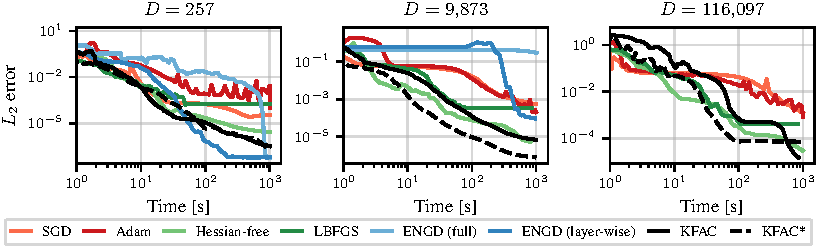
\includegraphics{kfac_pinns_exp/exp17_groupplot_poisson2d/l2_error_over_time.pdf}
  \caption{Performance of different optimizers on the 2d Poisson equation~\eqref{eq:2D-Poisson} measured in relative $L_2$ error against wall clock time for architectures with different parameter dimensions $D$.}
  \label{fig:2D-Poisson}
\end{figure}

We implement KFAC, KFAC*, and ENGD with either the per-layer or full Gramian in PyTorch~\citep{paszke2019pytorch}.
As a matrix-free version of ENGD, we use the Hessian-free optimizer~\citep{martens2010deep} which uses truncated conjugate gradients (CG) with exact Gramian-vector products to precondition the gradient.
We chose this because there is a fully-featured implementation from~\citet{tatzel2022late} which offers many additional heuristics like adaptive damping, CG backtracking, and backtracking line search, allowing this algorithm to work well with little hyper-parameter tuning.
As baselines, we use SGD with tuned learning rate and momentum, Adam with tuned learning rate, and LBFGS with tuned learning rate and history size.
We tune hyper-parameters using Weights \& Biases~\citep{wandb} (see \Cref{sec:tuning-protocol} for the exact protocol).
For random/grid search, we run an initial round of approximately 50 runs with generous search spaces, then narrow them down and re-run for another 50 runs; for Bayesian search, we assign the same total compute to each optimizer.
We report runs with lowest $L_2$ error estimated on a held-out data set with the known solution to the studied PDE.
To be comparable, all runs are executed on a compute cluster with RTX 6000 GPUs (24\,GiB RAM) in double precision, and we use the same computation time budget for all optimizers on a fixed PINN problem.
All search spaces and best run hyper-parameters, as well as training curves over iteration count rather than time, are in \Cref{sec:experimental_details}.

\textbf{Pedagogical example: 2d Poisson equation}
We start with a low-dimensional Poisson equation from~\citet{muller2023achieving} to reproduce ENGD's performance (\Cref{fig:2D-Poisson}).
It is given by
\begin{align}\label{eq:2D-Poisson}
  \begin{split}
    -\Delta u(x,y)
    &=
      2\pi^2 \sin(\pi x) \sin(\pi y) \quad \text{for } (x,y)\in[0,1]^2\,
    \\
    u(x,y)
    &=
      0 \quad \text{for } (x,y) \in\partial[0,1]^2.
  \end{split}
\end{align}
We choose a fixed data set of same size as the original paper, then use random/grid search to evaluate the performance of all optimizers for different $\tanh$-activated MLPs, one shallow and two with five fully-connected layers of different width (all details in \Cref{sec:2d-poisson-appendix}).
We include ENGD whenever the network's parameter space is small enough to build up the Gramian.

For the shallow net (\Cref{fig:2D-Poisson}, left), we can reproduce the results of~\cite{muller2023achieving}, where exact ENGD achieves high accuracy.
In terms of computation time, our KFACs are competitive with full-ENGD for a long phase, outperforming the first-order and quasi-Newton baselines.
In contrast to ENGD, which runs out of memory for networks with more than $\num{10000}$ parameters, KFAC scales to larger networks (\Cref{fig:2D-Poisson}, center and right) and is competitive with other second-order optimizers like Hessian-free, which uses more sophisticated heuristics.
We make similar observations on a small (1+1)d heat equation with the same models, see \Cref{sec:1d-heat-equation,fig:heat1d-appendix}.

\begin{figure}
  \centering
  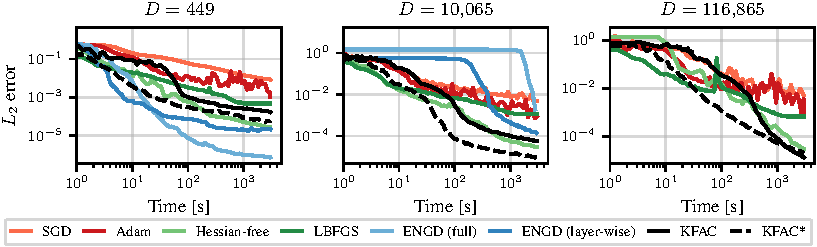
\includegraphics{kfac_pinns_exp/exp30_heat4d_groupplot/l2_error_over_time.pdf}
  \caption{Performance of different optimizers on the (4+1)d heat equation~\eqref{eq:4D-heat} measured in relative $L^2$ error against wall clock time for architectures with different parameter dimensions $D$.}
  \label{fig:4D-heat}
\end{figure}

\textbf{An evolutionary problem: (4+1)d heat equation}
To demonstrate that our methods can also be applied to other problems than the Poisson equation, we consider a four-dimensional heat equation
\begin{align}\label{eq:4D-heat}
  \begin{split}
    \partial_t u(t,\vx)-\kappa\Delta_\vx u(t,\vx)
    &=
      0 \quad \text{for } t\in[0,1], \vx\in [0,1]^{4}\,,
    \\
    u(0,\vx)
    &=
      \textstyle
      \sum_{i=1}^{4} \sin(2 x_i) \quad \text{for }
      \vx\in [0,1]^{4}\,,
    \\
    u(t,\vx)
    &=
      \textstyle
      \exp(-t) \sum_{i=1}^{4} \sin(2 x_i) \quad \text{for } t\in[0,1], \vx\in\partial[0,1]^{4}\,,
  \end{split}
\end{align}
with diffusivity constant $\kappa = \nicefrac{1}{4}$, similar to that studied in \cite{muller2023achieving} (see \Cref{sec:pinn-loss-heat-equation} for the heat equation's PINN loss).
We use the previous architectures with same hidden widths and evaluate optimizer performance with random/grid search (all details in \Cref{sec:4d-heat-app}), see \Cref{fig:4D-heat}.
To prevent over-fitting, we use mini-batches and sample a new batch each iteration.
We noticed that KFAC improves significantly when batches are sampled less frequently and hypothesize that it might need more iterations to make similar progress than one iteration of Hessian-free or ENGD on a batch.
Consequently we sample a new batch only every 100 iterations for KFAC.
To ensure that this does not lead to an unfair advantage for KFAC, we conduct an additional experiment for the MLP with $D=\num{116864}$ where we tune batch sizes, batch sampling frequencies, and all hyper-parameters with generous search spaces using Bayesian search (\Cref{sec:4d-heat-bayes-app}).
We find that this does not significantly boost performance of the other methods (compare \Cref{fig:4D-heat,fig:heat4d-bayes-appendix}).
Again, we observe that KFAC offers competitive performance compared to other second-order methods for networks with prohibitive size for ENGD and consistently outperforms SGD, Adam, and LBFGS.
We confirmed these observations with another 5d Poisson equation on the same architectures, see~\Cref{sec:poisson5d-appendix,fig:poisson5d-appendix}.

\begin{figure}
  \centering
  \includegraphics{kfac_pinns_exp/exp33_poisson_bayes_groupplot/l2_error_over_time.pdf}
  \caption{
    Optimizer performance on Poisson equations in high dimensions and different boundary conditions measured in relative $L_2$ error against wall clock time for networks with $D$ parameters.
  }
  \label{fig:10D-Poisson}
\end{figure}

\textbf{High-dimensional Poisson equations}
To demonstrate scaling to high-dimensional PDEs and even larger neural networks, we consider three Poisson equations ($d=5,10,100$) with different boundary conditions used in~\cite{yu2018deep, muller2023achieving}, which admit the solutions
\begin{align}\label{eq:solutions_poisson}
  \begin{split}
    u_\star(\vx)
    &=
      \textstyle
      \sum_{i=1}^5 \cos(\pi x_i) \quad \text{for } \vx\in [0,1]^{5}\,,
    \\
    u_\star(\vx)
    &=
      \textstyle
      \sum_{k=1}^5 x_{2k-1}x_{2k}  \quad \text{for } \vx\in [0,1]^{10}\,,
    \\
    u_\star(\vx)
    &=
      \lVert \vx \rVert_2^2 \quad \text{for } \vx\in [0,1]^{100}\,.
  \end{split}
\end{align}
We use the same architectures as before, but with larger intermediate widths and parameters up to a million (\Cref{fig:10D-Poisson}).
Due to lacking references for training such high-dimensional problems, we select all hyper-parameters via Bayesian search, including batch sizes and batch sampling frequencies (all details in \Cref{sec:high-dimensional-poissons-app}).
We see a similar picture as before with KFAC consistently outperforming first-order methods and LBFGS, offering competitive performance with Hessian-free.
To account for the possibility that the Bayesian search did not properly identify good hyper-parameters, we conduct a random/grid search experiment for the 10d Poisson equation (\Cref{fig:10D-Poisson}, middle), using similar batch sizes and same batch sampling frequencies as for the $(4+1)$d heat equation (all details in \Cref{sec:poisson10d-appendix}).
In this experiment, KFAC also achieved similar performance than Hessian-free and outperformed SGD, Adam, and LBFGS (\Cref{fig:poisson_10d-appendix}).

%%% Local Variables:
%%% mode: latex
%%% TeX-master: "../main"
%%% End:


\section{Discussion and Conclusion}\label{sec:conclusion}
We extended the concept of Kronecker-factored approximate curvature (KFAC) to Gauss-Newton matrices of Physics-informed neural network (PINN) losses that involve derivatives, rather than function evaluations, of the neural net.
This greatly reduces the computational cost of approximate natural gradient methods, which are known to work well on PINNs, and allows them to scale to much larger nets.
Our approach goes beyond the established KFAC for traditional supervised problems as it captures contributions from a PDE's differential operator that are crucial for optimization.
To establish KFAC for such losses, we use Taylor-mode autodiff to view the differential operator's compute graph as a forward net with shared weights, then apply the recently-developed formulation of KFAC for linear layers with weight sharing.
Empirically, we find that our KFAC-based optimizers are competitive with expensive second-order methods on small problems and scale to high-dimensional neural networks and PDEs while consistently outperforming first-order methods and LBFGS.

\textbf{Limitations \& future directions} While our implementation currently only supports MLPs and the Poisson and heat equations, the concepts we use to derive KFAC (Taylor-mode, weight sharing) apply to arbitrary architectures and PDEs, as described in~\Cref{sec:KFAC-general}.
We are excited that our current algorithms show promising performance when compared to second-order methods with sophisticated heuristics.
In fact, the original KFAC optimizer itself~\cite{martens2015optimizing} relies heavily on such heuristics that are said to be crucial for its performance~\cite{clarke2023adam}.
Our algorithms borrow components, but we did not explore all bells and whistles, e.g.\,adaptive damping and heuristics to distribute damping over the Kronecker factors.
We believe our current algorithm's performance can further be improved, e.g.\,by exploring (1) updating the KFAC matrices less frequently, as is standard for traditional KFAC, (2) merging the two Kronecker approximations for boundary and interior Gramians into a single one, (3) removing matrix inversions~\cite{lin2023simplifying}, (4) using structured Kronecker factors~\cite{lin2023structured}, (5) computing the Kronecker factors in parallel with the gradient~\cite{dangel2020backpack}, (6) using single or mixed precision training~\cite{micikevicius2017mixed}, and (7) studying cheaper KFAC flavours based on the empirical Fisher~\cite{kunstner2019limitations} or input-based curvature~\cite{benzing2022gradient,petersen2023isaac}.
%%% Local Variables:
%%% mode: latex
%%% TeX-master: "../main"
%%% End:

\begin{ack} % automatically suppressed in anonymized submission
  The authors thank Runa Eschenhagen for insightful discussions on KFAC for linear weight sharing layers.
  Resources used in preparing this research were provided, in part, by the Province of Ontario, the Government of Canada through CIFAR, and companies sponsoring Vector Institute.
  JM acknowledges funding by the Deutsche Forschungsgemeinschaft (DFG, German Research Foundation) under the project number 442047500 through the Collaborative Research Center \emph{Sparsity and Singular Structures} (SFB 1481).
\end{ack}
%%% Local Variables:
%%% mode: latex
%%% TeX-master: "../main"
%%% End:


\bibliography{references}
\bibliographystyle{icml2024.bst}

\clearpage
\appendix

\clearpage

% Use different numbering in appendix to make it clear that a
% section/table/algorithm is not in the main text
\renewcommand\thefigure{\thesection\arabic{figure}}
\renewcommand\thetable{\thesection\arabic{table}}
\renewcommand{\theequation}{\thesection\arabic{equation}}

% modified title header from main page, code extracted from NeurIPS template
\makeatletter
\vbox{%
  \hsize\textwidth
  \linewidth\hsize
  \vskip 0.1in
  \@toptitlebar
  \centering
  {\LARGE\bf \@title (Supplementary Material)\par}
  \@bottomtitlebar
  \vskip 0.3in \@minus 0.1in
}
\makeatother

% APPENDIX TOC
\startcontents[sections]
\printcontents[sections]{l}{1}{\setcounter{tocdepth}{2}}
\vspace{2em}

\section{Experimental Details and Additional Results}\label{sec:experimental_details}
\subsection{Hyper-Parameter Tuning Protocol}\label{sec:tuning-protocol}

In all our experiments, we tune the following optimizer hyper-parameters and otherwise use the PyTorch default values:
\begin{itemize}
\item \textbf{SGD:} learning rate, momentum
\item \textbf{Adam:} learning rate
\item \textbf{Hessian-free:} type of curvature matrix (Hessian or GGN), damping, whether to adapt damping over time (yes or no), maximum number of CG iterations
\item \textbf{LBFGS:} learning rate, history size
\item \textbf{ENGD:} damping, factor of the exponential moving average applied to the Gramian, initialization of the Gramian (zero or identity matrix)
\item \textbf{KFAC:} factor of the exponential moving average applied to the Kronecker factors, damping, momentum, initialization of the Kronecker factors (zero or identity matrix)
\item \textbf{KFAC*:} factor of the exponential moving average applied to the Kronecker factors, damping, initialization of the Kronecker factors (zero or identity matrix)
\end{itemize}

Depending on the optimizer and experiment we use grid, random, or Bayesian search from Weights \& Biases to determine the hyper-parameters.
Each individual run is executed in double precision and allowed to run for a given time budget, and we rank runs by the final $L_2$ error on a fixed evaluation data set. To allow comparison, all runs are executed on RTX 6000 GPUs with 24\,GiB of RAM. For grid and random searches, we use a round-based approach.
First, we choose a relatively wide search space and limit to approximately 50 runs.
In a second round, we narrow down the hyper-parameter space based on the first round, then re-run for another approximately 50 runs.
We will release the details of all hyper-parameter search spaces, as well as the hyper-parameters for the best runs in our implementation.

\subsection{2d Poisson Equation}\label{sec:2d-poisson-appendix}

\paragraph{Setup} We consider a two-dimensional Poisson equation $-\Delta u(x, y) = 2 \pi^2 \sin(\pi x) \sin(\pi y)$ on the unit square $(x,y) \in [0, 1]^2$ with sine product right-hand side and zero boundary conditions $u(x, y) = 0$ for $(x,y) \in \partial [0,1]^2$.
We choose a single set of training points with $N_{\Omega} = 900, N_{\partial\Omega} = 120$.
The $L_2$ error is evaluated on a separate set of $\num{9000}$ data points using the known solution $u_{\star}(x, y) = \sin(\pi x) \sin(\pi y)$.
Each run is limited to a compute time of $\num{1000}\,\text{s}$.
We compare three MLP architectures of increasing size, each of whose linear layers are Tanh-activated except for the final one: a shallow $2\to 64\to 1$ MLP with $D=257$ trainable parameters, a five layer $2 \to 64 \to 64 \to 48 \to 48 \to 1$ MLP with $D=\num{9873}$ trainable parameters, and a five layer $2 \to 256 \to 256\to 128 \to 128 \to 1$ MLP with $D=\num{116097}$ trainable parameters.
For the biggest architecture, full and per-layer ENGD lead to out-of-memory errors and are thus not tested in the experiments.
\Cref{fig:poisson2d-appendix} visualizes the results, and \Cref{fig:2d-poisson-visualization} illustrates the learned solutions over training for all optimizers on the shallow MLP.

\begin{figure}[!h]
  \centering
  \def\pathToFigs{kfac_pinns_exp/exp17_groupplot_poisson2d}
  \begin{subfigure}[t]{1.0\linewidth}
    \caption{}\label{subfig:poisson2d-time}
    % trim legend, xlabel and xticklabels
    % [trim={left bottom right top},clip]
    \includegraphics[trim={0 1.3cm 0 0},clip]{\pathToFigs/l2_error_over_time.pdf}
    % trim the legend and titles
    % [trim={left bottom right top},clip]
    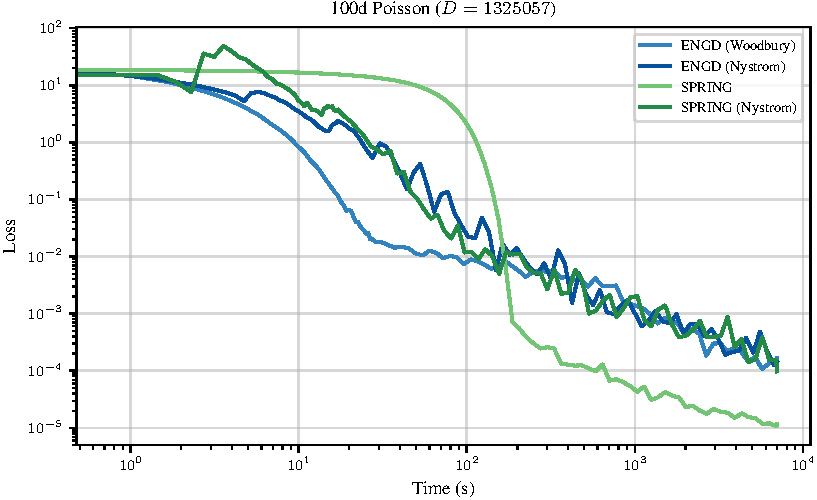
\includegraphics[trim={0 0.8cm 0 0.3cm},clip]{\pathToFigs/loss_over_time.pdf}
  \end{subfigure}
  \begin{subfigure}[t]{1.0\linewidth}
    \caption{}\label{subfig:poisson2d-step}
    % trim the legend, xlabel and xticklabels
    % [trim={left bottom right top},clip]
    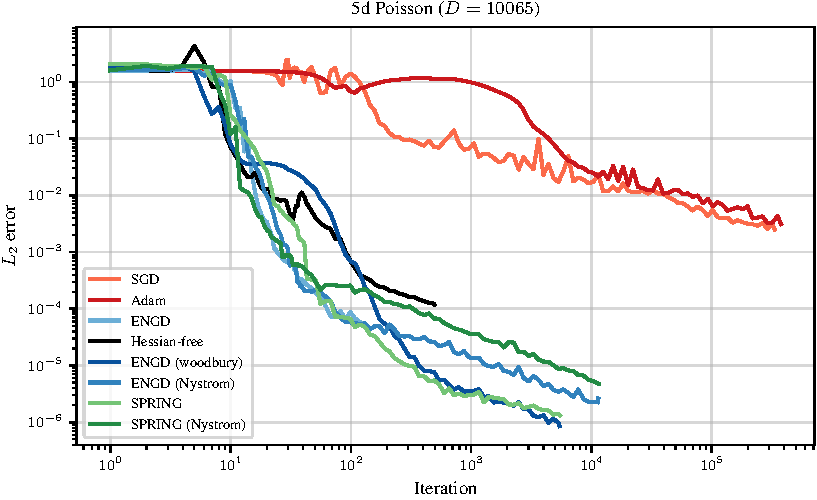
\includegraphics[trim={0 1.3cm 0 0.3cm},clip]{\pathToFigs/l2_error_over_step.pdf}
    % trim the titles
    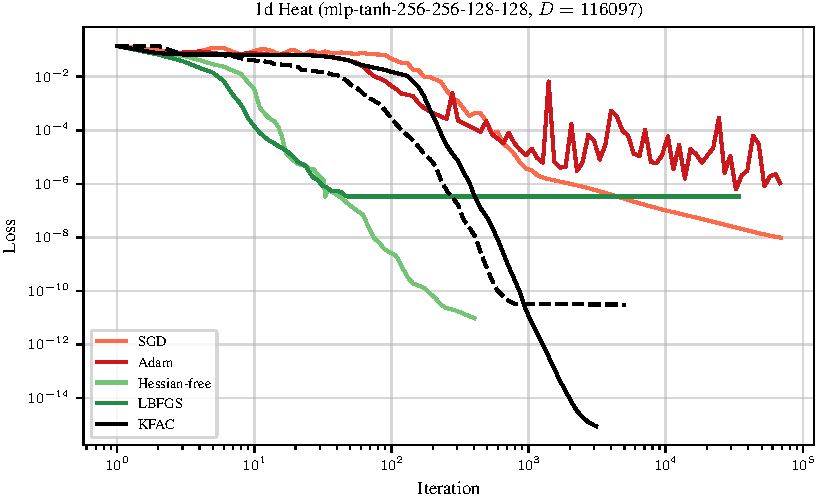
\includegraphics[trim={0 0 0 0.3cm},clip]{\pathToFigs/loss_over_step.pdf}
  \end{subfigure}
  \caption{ Training loss and evaluation $L_2$ error for learning the solution to a 2d Poisson equation over (\subref{subfig:poisson2d-time}) time and (\subref{subfig:poisson2d-step}) steps.
    Columns are different neural networks.}\label{fig:poisson2d-appendix}
\end{figure}

\begin{table}[!h]
  \centering
  \def\pathToRuns{kfac_pinns_exp/exp42_visualize_solutions/visualize_solution}
  \renewcommand\tabularxcolumn[1]{>{\Centering}m{#1}}
  \begin{small}
    \begin{tabularx}{\textwidth}{XXXXXX}
      \textbf{Optimizer} & \textbf{First step} & \textbf{0.1\% trained} & \textbf{1\% trained} & \textbf{10\% trained} & \textbf{True solution}
      \\
      SGD
      % [trim={left bottom right top},clip]
      &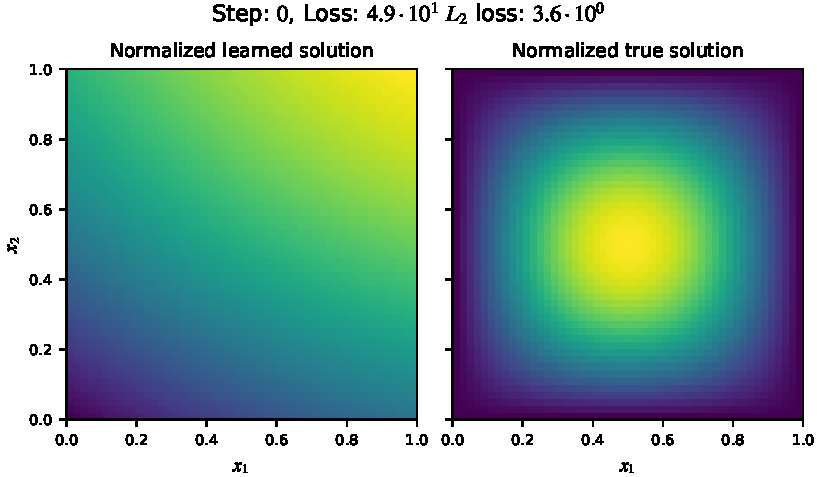
\includegraphics[trim={0.9cm 0.8cm 6.5cm 1.0cm},clip,scale=0.31]{\pathToRuns/SGD/poisson_2d_sin_product_mlp-tanh-64_SGD_step0000000.pdf}
      &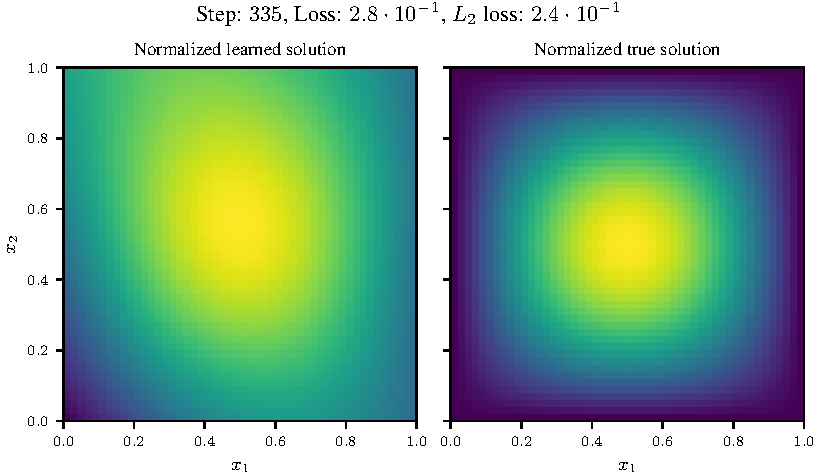
\includegraphics[trim={0.9cm 0.8cm 6.5cm 1.0cm},clip,scale=0.31]{\pathToRuns/SGD/poisson_2d_sin_product_mlp-tanh-64_SGD_step0000335.pdf}
      &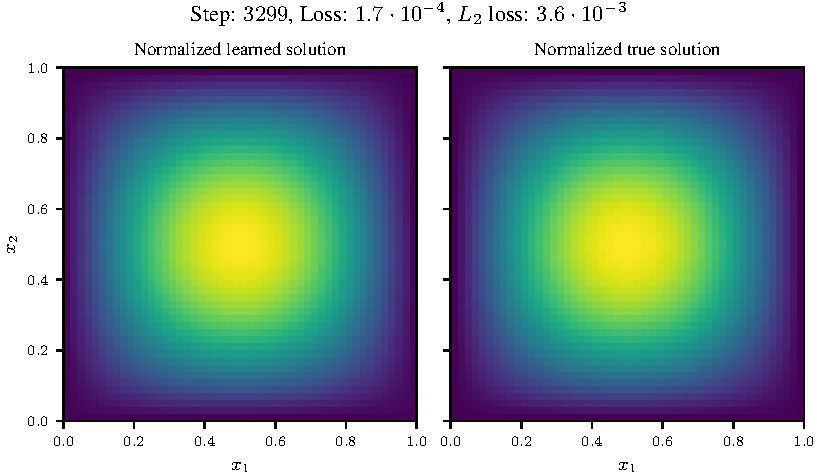
\includegraphics[trim={0.9cm 0.8cm 6.5cm 1.0cm},clip,scale=0.31]{\pathToRuns/SGD/poisson_2d_sin_product_mlp-tanh-64_SGD_step0003299.pdf}
      &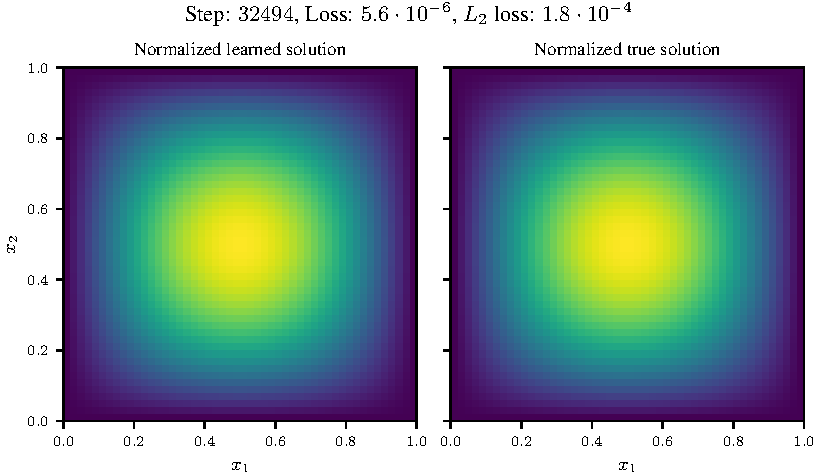
\includegraphics[trim={0.9cm 0.8cm 6.5cm 1.0cm},clip,scale=0.31]{\pathToRuns/SGD/poisson_2d_sin_product_mlp-tanh-64_SGD_step0032494.pdf}
      &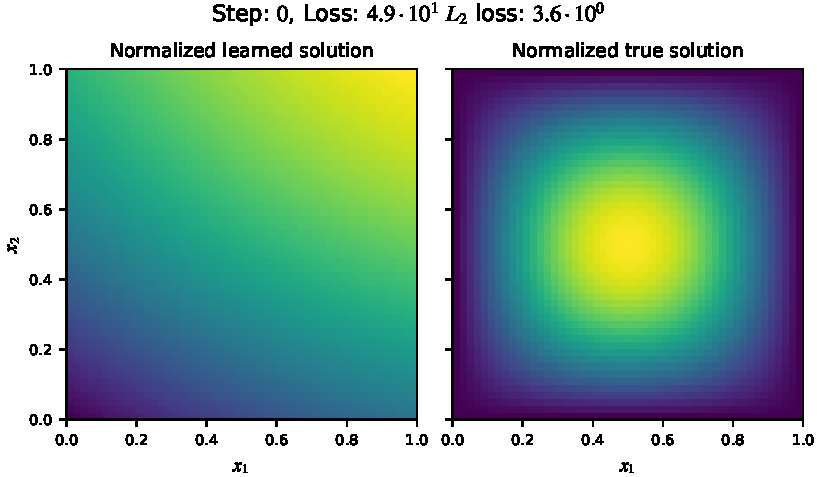
\includegraphics[trim={7.25cm 0.8cm 0 1.0cm},clip,scale=0.31]{\pathToRuns/SGD/poisson_2d_sin_product_mlp-tanh-64_SGD_step0000000.pdf}
      \\
      Adam
      % [trim={left bottom right top},clip]
      &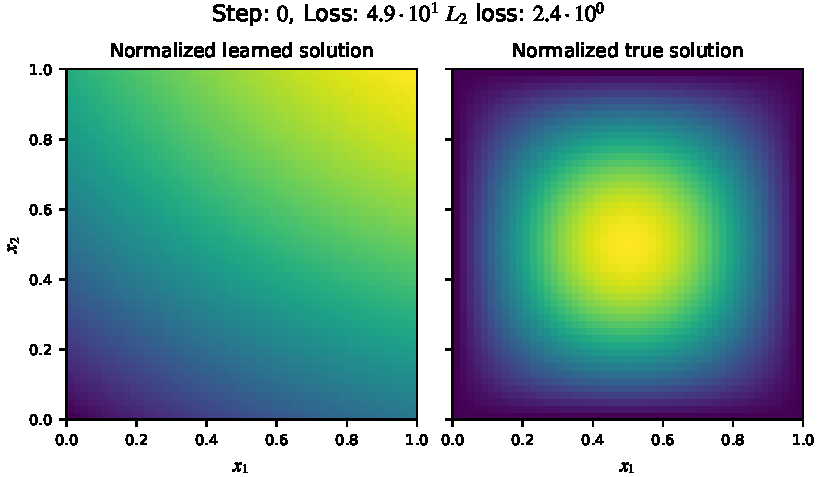
\includegraphics[trim={0.9cm 0.8cm 6.5cm 1.0cm},clip,scale=0.31]{\pathToRuns/Adam/poisson_2d_sin_product_mlp-tanh-64_Adam_step0000000.pdf}
      &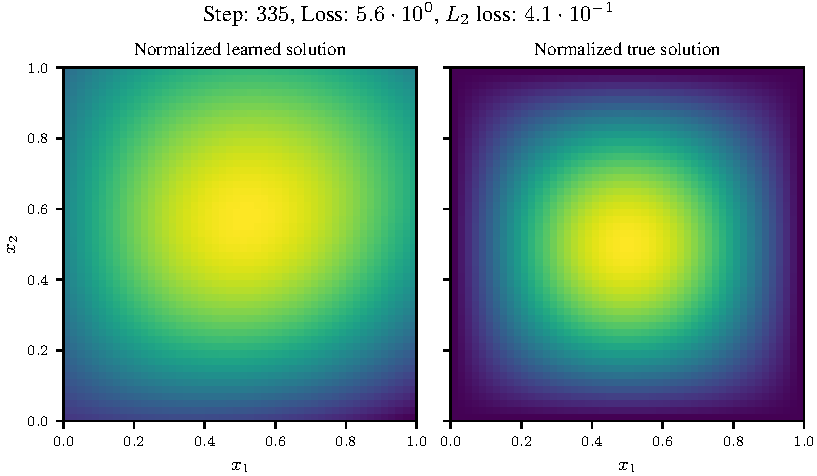
\includegraphics[trim={0.9cm 0.8cm 6.5cm 1.0cm},clip,scale=0.31]{\pathToRuns/Adam/poisson_2d_sin_product_mlp-tanh-64_Adam_step0000335.pdf}
      &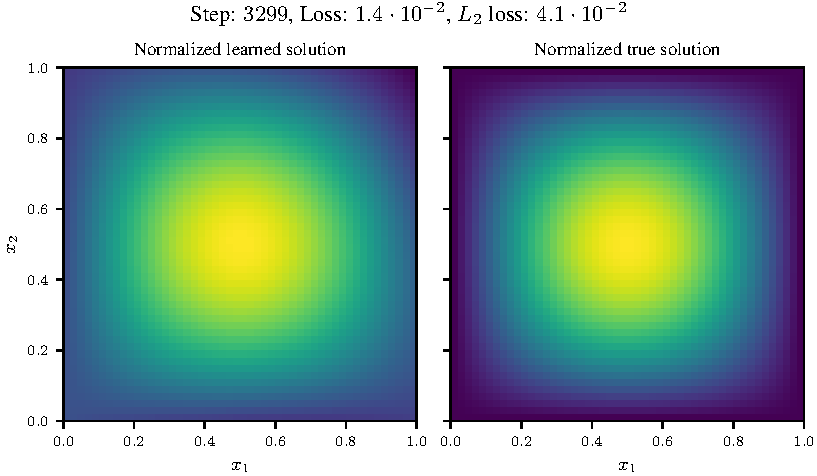
\includegraphics[trim={0.9cm 0.8cm 6.5cm 1.0cm},clip,scale=0.31]{\pathToRuns/Adam/poisson_2d_sin_product_mlp-tanh-64_Adam_step0003299.pdf}
      &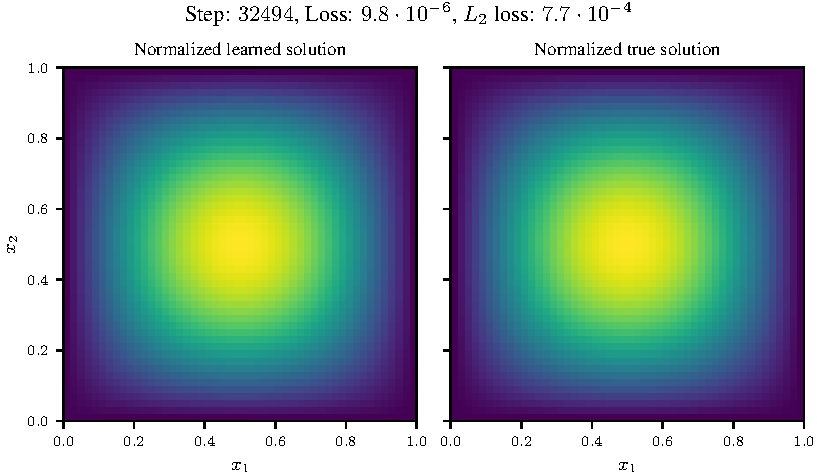
\includegraphics[trim={0.9cm 0.8cm 6.5cm 1.0cm},clip,scale=0.31]{\pathToRuns/Adam/poisson_2d_sin_product_mlp-tanh-64_Adam_step0032494.pdf}
      &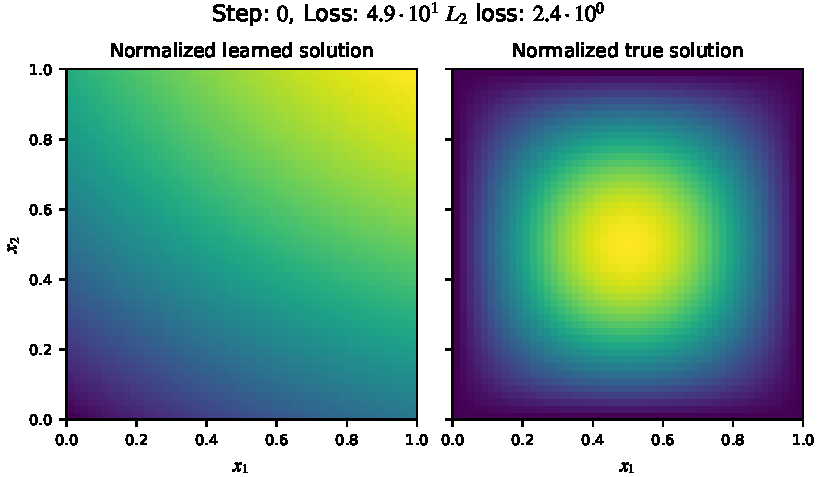
\includegraphics[trim={7.25cm 0.8cm 0 1.0cm},clip,scale=0.31]{\pathToRuns/Adam/poisson_2d_sin_product_mlp-tanh-64_Adam_step0000000.pdf}
      \\
      % [trim={left bottom right top},clip]
      LBFGS
      & 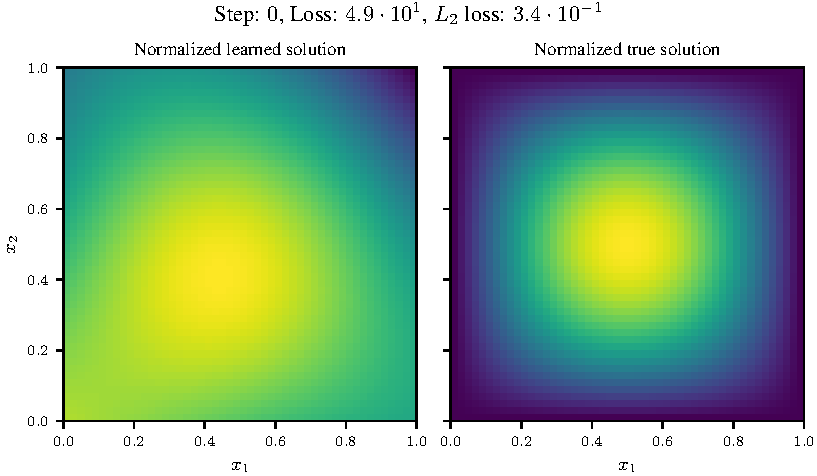
\includegraphics[trim={0.9cm 0.8cm 6.5cm 1.0cm},clip,scale=0.31]{\pathToRuns/LBFGS/poisson_2d_sin_product_mlp-tanh-64_LBFGS_step0000000.pdf}
      & 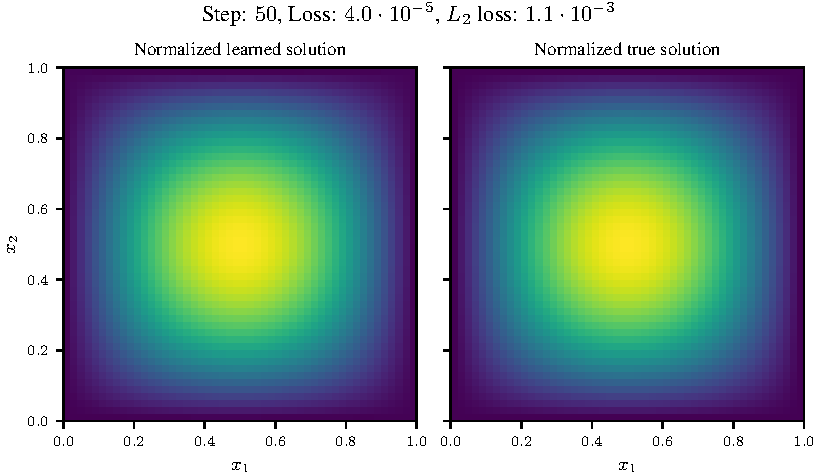
\includegraphics[trim={0.9cm 0.8cm 6.5cm 1.0cm},clip,scale=0.31]{\pathToRuns/LBFGS/poisson_2d_sin_product_mlp-tanh-64_LBFGS_step0000050.pdf}
      & 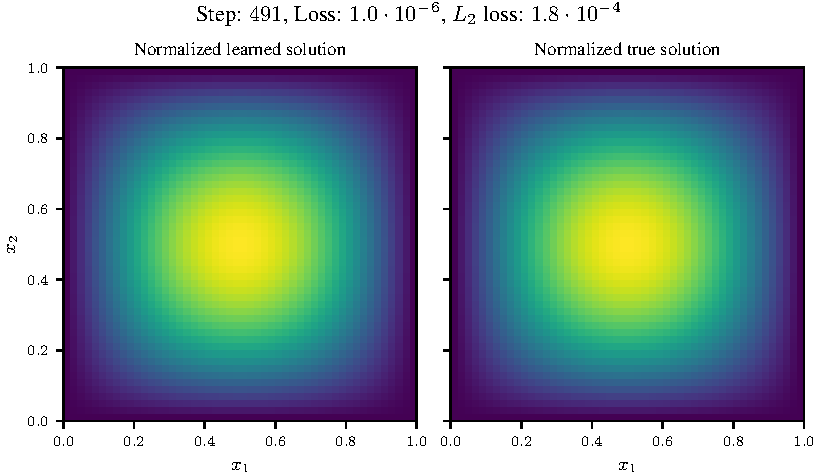
\includegraphics[trim={0.9cm 0.8cm 6.5cm 1.0cm},clip,scale=0.31]{\pathToRuns/LBFGS/poisson_2d_sin_product_mlp-tanh-64_LBFGS_step0000491.pdf}
      & 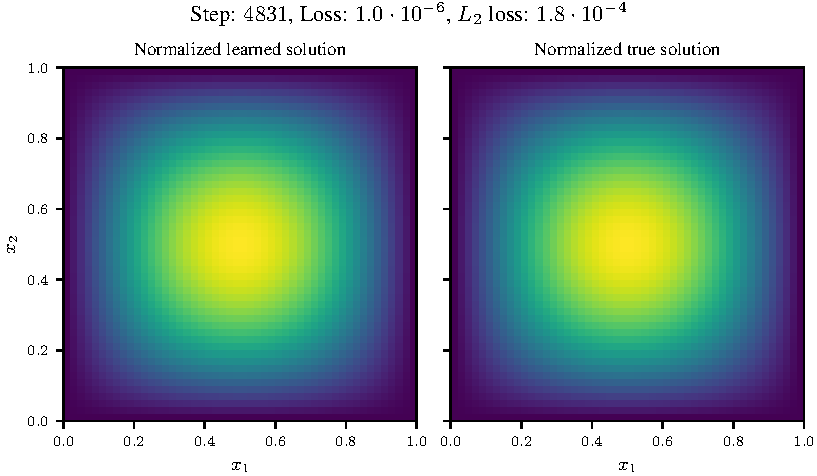
\includegraphics[trim={0.9cm 0.8cm 6.5cm 1.0cm},clip,scale=0.31]{\pathToRuns/LBFGS/poisson_2d_sin_product_mlp-tanh-64_LBFGS_step0004831.pdf}
      & 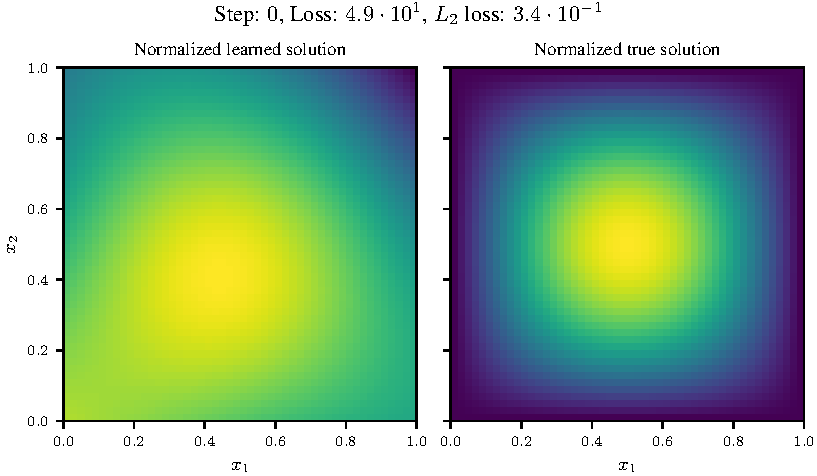
\includegraphics[trim={7.25cm 0.8cm 0 1.0cm},clip,scale=0.31]{\pathToRuns/LBFGS/poisson_2d_sin_product_mlp-tanh-64_LBFGS_step0000000.pdf}
      \\
      Hessian-free
      % [trim={left bottom right top},clip]
      &\includegraphics[trim={0.9cm 0.8cm 6.5cm 1.0cm},clip,scale=0.31]{\pathToRuns/Hessian-free/poisson_2d_sin_product_mlp-tanh-64_Hessianfree_step0000000.pdf}
      &\includegraphics[trim={0.9cm 0.8cm 6.5cm 1.0cm},clip,scale=0.31]{\pathToRuns/Hessian-free/poisson_2d_sin_product_mlp-tanh-64_Hessianfree_step0000004.pdf}
      &\includegraphics[trim={0.9cm 0.8cm 6.5cm 1.0cm},clip,scale=0.31]{\pathToRuns/Hessian-free/poisson_2d_sin_product_mlp-tanh-64_Hessianfree_step0000035.pdf}
      &\includegraphics[trim={0.9cm 0.8cm 6.5cm 1.0cm},clip,scale=0.31]{\pathToRuns/Hessian-free/poisson_2d_sin_product_mlp-tanh-64_Hessianfree_step0000335.pdf}
      &\includegraphics[trim={7.25cm 0.8cm 0 1.0cm},clip,scale=0.31]{\pathToRuns/Hessian-free/poisson_2d_sin_product_mlp-tanh-64_Hessianfree_step0000000.pdf}
      \\
      % [trim={left bottom right top},clip]
      ENGD (full)
      &\includegraphics[trim={0.9cm 0.8cm 6.5cm 1.0cm},clip,scale=0.31]{\pathToRuns/ENGD_full/poisson_2d_sin_product_mlp-tanh-64_ENGD_step0000000.pdf}
      &\includegraphics[trim={0.9cm 0.8cm 6.5cm 1.0cm},clip,scale=0.31]{\pathToRuns/ENGD_full/poisson_2d_sin_product_mlp-tanh-64_ENGD_step0000006.pdf}
      &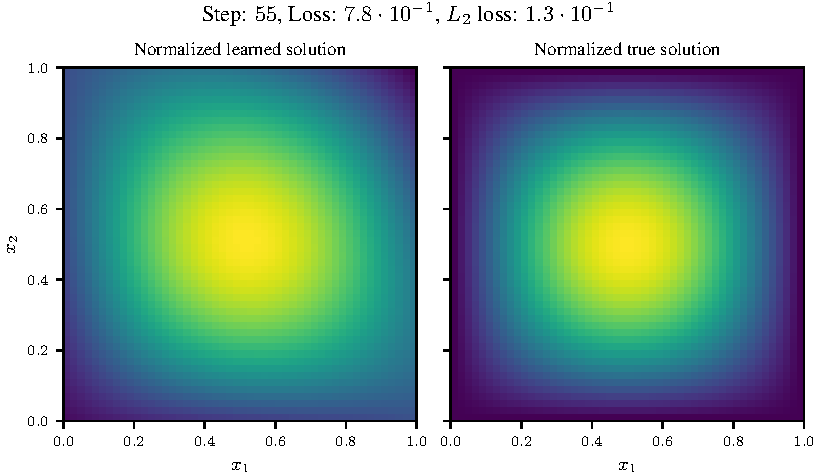
\includegraphics[trim={0.9cm 0.8cm 6.5cm 1.0cm},clip,scale=0.31]{\pathToRuns/ENGD_full/poisson_2d_sin_product_mlp-tanh-64_ENGD_step0000055.pdf}
      &\includegraphics[trim={0.9cm 0.8cm 6.5cm 1.0cm},clip,scale=0.31]{\pathToRuns/ENGD_full/poisson_2d_sin_product_mlp-tanh-64_ENGD_step0000594.pdf}
      &\includegraphics[trim={7.25cm 0.8cm 0 1.0cm},clip,scale=0.31]{\pathToRuns/ENGD_full/poisson_2d_sin_product_mlp-tanh-64_ENGD_step0000000.pdf}
      \\
      ENGD (layer-wise)
      % [trim={left bottom right top},clip]
      &\includegraphics[trim={0.9cm 0.8cm 6.5cm 1.0cm},clip,scale=0.31]{\pathToRuns/ENGD_layer-wise/poisson_2d_sin_product_mlp-tanh-64_ENGD_step0000000.pdf}
      &\includegraphics[trim={0.9cm 0.8cm 6.5cm 1.0cm},clip,scale=0.31]{\pathToRuns/ENGD_layer-wise/poisson_2d_sin_product_mlp-tanh-64_ENGD_step0000006.pdf}
      &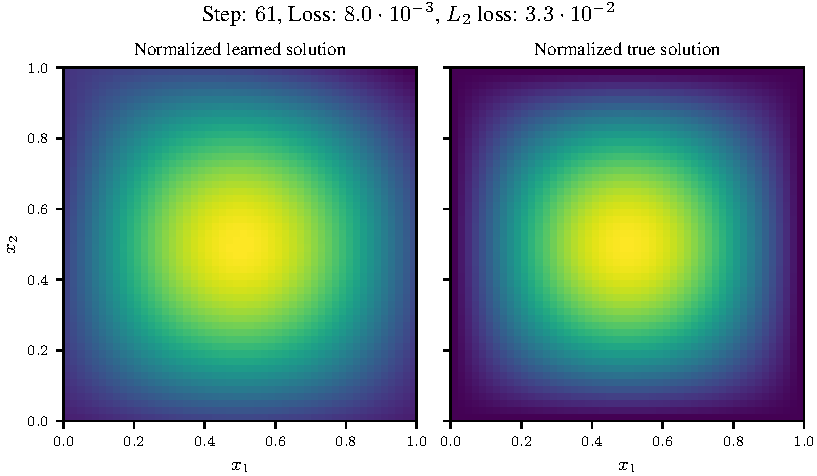
\includegraphics[trim={0.9cm 0.8cm 6.5cm 1.0cm},clip,scale=0.31]{\pathToRuns/ENGD_layer-wise/poisson_2d_sin_product_mlp-tanh-64_ENGD_step0000061.pdf}
      &\includegraphics[trim={0.9cm 0.8cm 6.5cm 1.0cm},clip,scale=0.31]{\pathToRuns/ENGD_layer-wise/poisson_2d_sin_product_mlp-tanh-64_ENGD_step0000594.pdf}
      &\includegraphics[trim={7.25cm 0.8cm 0 1.0cm},clip,scale=0.31]{\pathToRuns/ENGD_layer-wise/poisson_2d_sin_product_mlp-tanh-64_ENGD_step0000000.pdf}
      \\
      KFAC
      % [trim={left bottom right top},clip]
      &\includegraphics[trim={0.9cm 0.8cm 6.5cm 1.0cm},clip,scale=0.31]{\pathToRuns/KFAC/poisson_2d_sin_product_mlp-tanh-64_KFAC_step0000000.pdf}
      &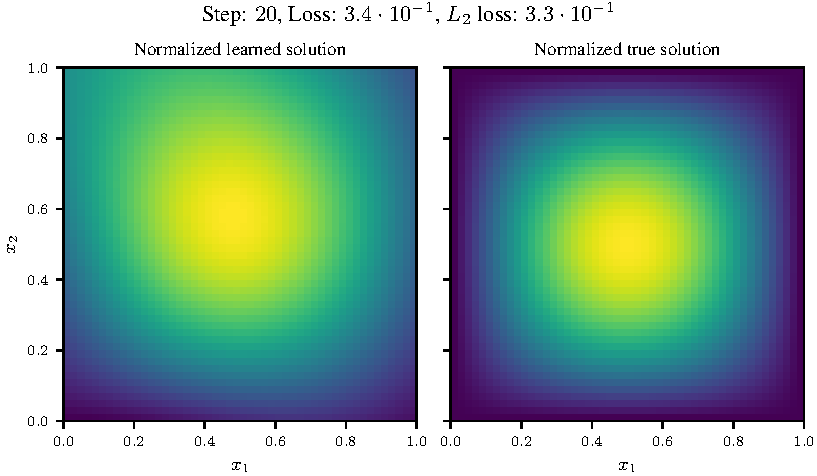
\includegraphics[trim={0.9cm 0.8cm 6.5cm 1.0cm},clip,scale=0.31]{\pathToRuns/KFAC/poisson_2d_sin_product_mlp-tanh-64_KFAC_step0000020.pdf}
      &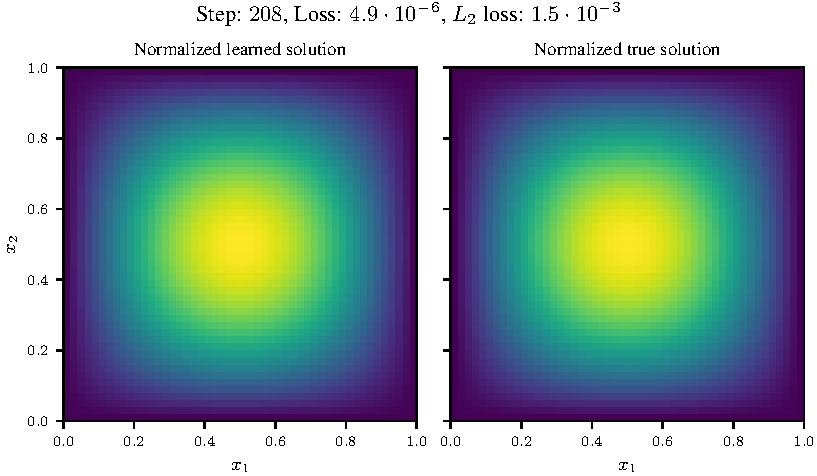
\includegraphics[trim={0.9cm 0.8cm 6.5cm 1.0cm},clip,scale=0.31]{\pathToRuns/KFAC/poisson_2d_sin_product_mlp-tanh-64_KFAC_step0000208.pdf}
      &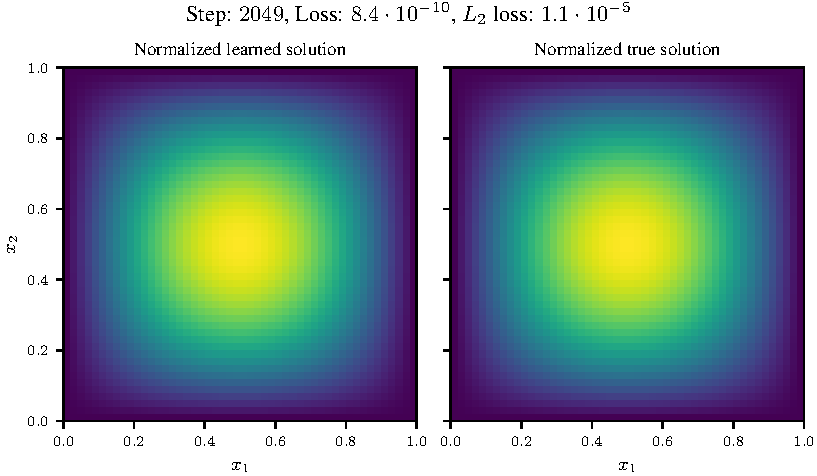
\includegraphics[trim={0.9cm 0.8cm 6.5cm 1.0cm},clip,scale=0.31]{\pathToRuns/KFAC/poisson_2d_sin_product_mlp-tanh-64_KFAC_step0002049.pdf}
      &\includegraphics[trim={7.25cm 0.8cm 0 1.0cm},clip,scale=0.31]{\pathToRuns/KFAC/poisson_2d_sin_product_mlp-tanh-64_KFAC_step0000000.pdf}
      \\
      KFAC*
      % [trim={left bottom right top},clip]
      &\includegraphics[trim={0.9cm 0.8cm 6.5cm 1.0cm},clip,scale=0.31]{\pathToRuns/KFAC_auto/poisson_2d_sin_product_mlp-tanh-64_KFAC_step0000000.pdf}
      &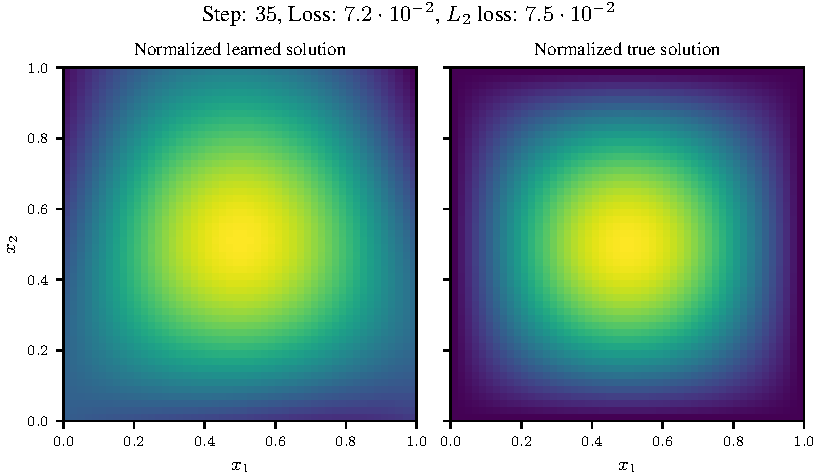
\includegraphics[trim={0.9cm 0.8cm 6.5cm 1.0cm},clip,scale=0.31]{\pathToRuns/KFAC_auto/poisson_2d_sin_product_mlp-tanh-64_KFAC_step0000035.pdf}
      &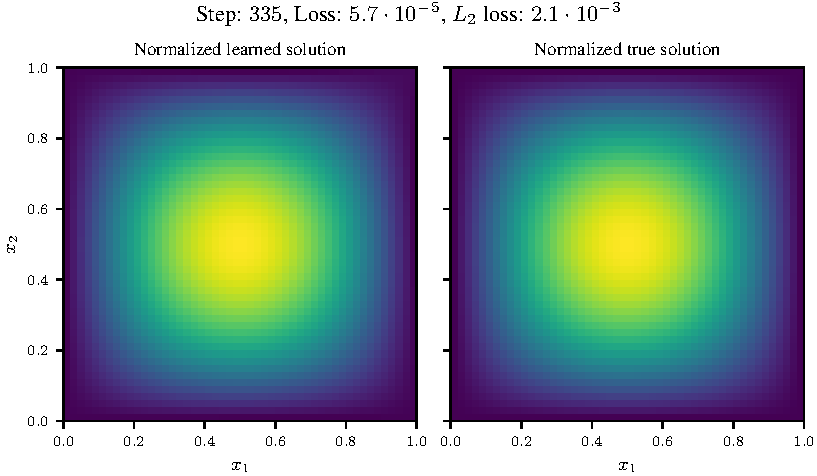
\includegraphics[trim={0.9cm 0.8cm 6.5cm 1.0cm},clip,scale=0.31]{\pathToRuns/KFAC_auto/poisson_2d_sin_product_mlp-tanh-64_KFAC_step0000335.pdf}
      &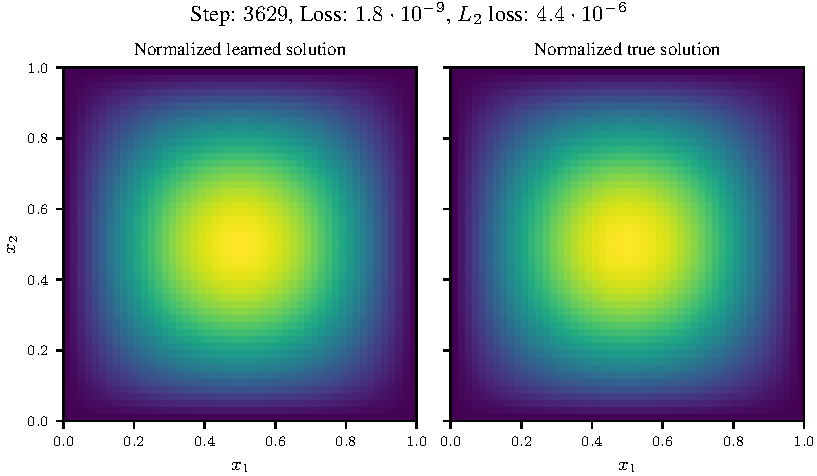
\includegraphics[trim={0.9cm 0.8cm 6.5cm 1.0cm},clip,scale=0.31]{\pathToRuns/KFAC_auto/poisson_2d_sin_product_mlp-tanh-64_KFAC_step0003629.pdf}
      &\includegraphics[trim={7.25cm 0.8cm 0 1.0cm},clip,scale=0.31]{\pathToRuns/KFAC_auto/poisson_2d_sin_product_mlp-tanh-64_KFAC_step0000000.pdf}
    \end{tabularx}
  \end{small}
  \captionof{figure}{Visual comparison learned and true solutions while training with different optimizers for the 2d Poisson equation using a two-layer MLP (corresponding to the curves in \Cref{fig:2D-Poisson} left).
    All functions are shown on the unit square $(x, y) \in \Omega = [0; 1]^2$ and normalized to the unit interval.}
  \label{fig:2d-poisson-visualization}
\end{table}

\paragraph{Best run details}
The runs shown in \Cref{fig:poisson2d-appendix} correspond to the following hyper-parameters:
\begin{itemize}
\item $2\to 64\to 1$ MLP with $D=257$
  \begin{itemize}
    \def\pathToRuns{kfac_pinns_exp/exp09_reproduce_poisson2d/tex}
  \item \textbf{SGD:} learning rate: $\num[scientific-notation=true]{2.686653e-04}$, momentum: $\num[scientific-notation=true]{9.878243e-01}$, $N_{\Omega}$: $\num[scientific-notation=false]{606}$, $N_{\partial\Omega}$: $\num[scientific-notation=false]{2001}$, batch sampling frequency: $\num[scientific-notation=false]{1570}$
  \item \textbf{Adam:} learning rate: $\num[scientific-notation=true]{5.416376e-04}$
  \item \textbf{Hessian-free:} curvature matrix: $\text{GGN}$, initial damping: $\num[scientific-notation=true]{0.1}$, constant damping: $\text{no}$, maximum CG iterations: $\num[scientific-notation=false]{250}$
  \item \textbf{LBFGS:} learning rate: $\num[scientific-notation=true]{0.2}$, history size: $\num[scientific-notation=false]{225}$
  \item \textbf{ENGD (full):} damping: $\num[scientific-notation=true]{1e-08}$, exponential moving average: $\num[scientific-notation=false]{0}$, initialize Gramian to identity: $\text{yes}$
  \item \textbf{ENGD (layer-wise):} damping: $\num[scientific-notation=true]{1e-06}$, exponential moving average: $\num[scientific-notation=false]{0}$, initialize Gramian to identity: $\text{yes}$
  \item \textbf{KFAC:} damping: $\num[scientific-notation=true]{3.169186e-13}$, momentum: $\num[scientific-notation=true]{7.075879e-01}$, exponential moving average: $\num[scientific-notation=true]{8.860410e-01}$, initialize Kronecker factors to identity: $\text{yes}$
  \item \textbf{KFAC*:} damping: $\num[scientific-notation=true]{2.965060e-08}$, exponential moving average: $\num[scientific-notation=true]{9.574717e-01}$, initialize Kronecker factors to identity: $\text{yes}$
  \end{itemize}

\item $2 \to 64 \to 64 \to 48 \to 48 \to 1$ MLP with $D=\num{9873}$
  \begin{itemize}
    \def\pathToRuns{kfac_pinns_exp/exp15_poisson2d_deepwide/tex}
  \item \textbf{SGD:} learning rate: $\num[scientific-notation=true]{2.686653e-04}$, momentum: $\num[scientific-notation=true]{9.878243e-01}$, $N_{\Omega}$: $\num[scientific-notation=false]{606}$, $N_{\partial\Omega}$: $\num[scientific-notation=false]{2001}$, batch sampling frequency: $\num[scientific-notation=false]{1570}$
  \item \textbf{Adam:} learning rate: $\num[scientific-notation=true]{5.416376e-04}$
  \item \textbf{Hessian-free:} curvature matrix: $\text{GGN}$, initial damping: $\num[scientific-notation=true]{0.1}$, constant damping: $\text{no}$, maximum CG iterations: $\num[scientific-notation=false]{250}$
  \item \textbf{LBFGS:} learning rate: $\num[scientific-notation=true]{0.2}$, history size: $\num[scientific-notation=false]{225}$
  \item \textbf{ENGD (full):} damping: $\num[scientific-notation=true]{1e-08}$, exponential moving average: $\num[scientific-notation=false]{0}$, initialize Gramian to identity: $\text{yes}$
  \item \textbf{ENGD (layer-wise):} damping: $\num[scientific-notation=true]{1e-06}$, exponential moving average: $\num[scientific-notation=false]{0}$, initialize Gramian to identity: $\text{yes}$
  \item \textbf{KFAC:} damping: $\num[scientific-notation=true]{3.169186e-13}$, momentum: $\num[scientific-notation=true]{7.075879e-01}$, exponential moving average: $\num[scientific-notation=true]{8.860410e-01}$, initialize Kronecker factors to identity: $\text{yes}$
  \item \textbf{KFAC*:} damping: $\num[scientific-notation=true]{2.965060e-08}$, exponential moving average: $\num[scientific-notation=true]{9.574717e-01}$, initialize Kronecker factors to identity: $\text{yes}$
  \end{itemize}

\item $2 \to 256 \to 256\to 128 \to 128 \to 1$ MLP with $D=\num{116097}$
  \begin{itemize}
    \def\pathToRuns{kfac_pinns_exp/exp20_poisson2d_mlp_tanh_256/tex}
  \item \textbf{SGD:} learning rate: $\num[scientific-notation=true]{2.686653e-04}$, momentum: $\num[scientific-notation=true]{9.878243e-01}$, $N_{\Omega}$: $\num[scientific-notation=false]{606}$, $N_{\partial\Omega}$: $\num[scientific-notation=false]{2001}$, batch sampling frequency: $\num[scientific-notation=false]{1570}$
  \item \textbf{Adam:} learning rate: $\num[scientific-notation=true]{5.416376e-04}$
  \item \textbf{Hessian-free:} curvature matrix: $\text{GGN}$, initial damping: $\num[scientific-notation=true]{0.1}$, constant damping: $\text{no}$, maximum CG iterations: $\num[scientific-notation=false]{250}$
  \item \textbf{LBFGS:} learning rate: $\num[scientific-notation=true]{0.2}$, history size: $\num[scientific-notation=false]{225}$
  \item \textbf{KFAC:} damping: $\num[scientific-notation=true]{3.169186e-13}$, momentum: $\num[scientific-notation=true]{7.075879e-01}$, exponential moving average: $\num[scientific-notation=true]{8.860410e-01}$, initialize Kronecker factors to identity: $\text{yes}$
  \item \textbf{KFAC*:} damping: $\num[scientific-notation=true]{2.965060e-08}$, exponential moving average: $\num[scientific-notation=true]{9.574717e-01}$, initialize Kronecker factors to identity: $\text{yes}$
  \end{itemize}
\end{itemize}

\paragraph{Search space details} The runs shown in \Cref{fig:poisson2d-appendix} were determined to be the best via a search with approximately 50 runs on the following search spaces which were obtained by refining an initially wider search ($\mathcal{U}$ denotes a uniform, and $\mathcal{LU}$ a log-uniform distribution):
\begin{itemize}
\item $2\to 64\to 1$ MLP with $D=257$
  \begin{itemize}
    \def\pathToRuns{kfac_pinns_exp/exp09_reproduce_poisson2d/tex}
  \item \textbf{SGD:} learning rate: $\mathcal{LU}([\num[scientific-notation=true]{1e-06}; \num[scientific-notation=false]{1}])$, momentum: $\mathcal{U}([\num[scientific-notation=false]{0}; \num[scientific-notation=true]{0.99}])$, $N_{\Omega}$: $\mathcal{U}(\{\num[scientific-notation=false]{100},\num[scientific-notation=false]{101},\text{\dots},\num[scientific-notation=false]{10000}\})$, $N_{\partial\Omega}$: $\mathcal{U}(\{\num[scientific-notation=false]{50},\num[scientific-notation=false]{51},\text{\dots},\num[scientific-notation=false]{5000}\})$, batch sampling frequency: $\mathcal{U}(\{\num[scientific-notation=false]{0},\num[scientific-notation=false]{1},\text{\dots},\num[scientific-notation=false]{10000}\})$
  \item \textbf{Adam:} learning rate: $\mathcal{LU}([\num[scientific-notation=true]{1e-06}; \num[scientific-notation=false]{1}])$, $N_{\Omega}$: $\mathcal{U}(\{\num[scientific-notation=false]{100},\num[scientific-notation=false]{101},\text{\dots},\num[scientific-notation=false]{5000}\})$, $N_{\partial\Omega}$: $\mathcal{U}(\{\num[scientific-notation=false]{50},\num[scientific-notation=false]{51},\text{\dots},\num[scientific-notation=false]{2500}\})$, batch sampling frequency: $\mathcal{U}(\{\num[scientific-notation=false]{0},\num[scientific-notation=false]{1},\text{\dots},\num[scientific-notation=false]{1000}\})$
  \item \textbf{Hessian-free:} curvature matrix: $\mathcal{U}(\{\text{GGN},\text{Hessian}\})$, initial damping: $\mathcal{LU}([\num[scientific-notation=true]{1e-15}; \num[scientific-notation=false]{1}])$, constant damping: $\mathcal{U}(\{\text{no},\text{yes}\})$, maximum CG iterations: $\mathcal{U}(\{\num[scientific-notation=false]{1},\num[scientific-notation=false]{2},\text{\dots},\num[scientific-notation=false]{500}\})$, $N_{\Omega}$: $\mathcal{U}(\{\num[scientific-notation=false]{100},\num[scientific-notation=false]{101},\text{\dots},\num[scientific-notation=false]{10000}\})$, $N_{\partial\Omega}$: $\mathcal{U}(\{\num[scientific-notation=false]{50},\num[scientific-notation=false]{51},\text{\dots},\num[scientific-notation=false]{5000}\})$, batch sampling frequency: $\mathcal{U}(\{\num[scientific-notation=false]{0},\num[scientific-notation=false]{1},\text{\dots},\num[scientific-notation=false]{10000}\})$
  \item \textbf{LBFGS:} learning rate: $\mathcal{LU}([\num[scientific-notation=true]{1e-06}; \num[scientific-notation=false]{1}])$, history size: $\mathcal{U}(\{\num[scientific-notation=false]{5},\num[scientific-notation=false]{6},\text{\dots},\num[scientific-notation=false]{500}\})$, $N_{\Omega}$: $\mathcal{U}(\{\num[scientific-notation=false]{100},\num[scientific-notation=false]{101},\text{\dots},\num[scientific-notation=false]{5000}\})$, $N_{\partial\Omega}$: $\mathcal{U}(\{\num[scientific-notation=false]{50},\num[scientific-notation=false]{51},\text{\dots},\num[scientific-notation=false]{2500}\})$, batch sampling frequency: $\mathcal{U}(\{\num[scientific-notation=false]{0},\num[scientific-notation=false]{1},\text{\dots},\num[scientific-notation=false]{5000}\})$
  \item \textbf{ENGD (full):} damping: $\mathcal{U}(\{\num[scientific-notation=true]{1e-06},\num[scientific-notation=true]{1e-08},\num[scientific-notation=true]{1e-10},\num[scientific-notation=true]{1e-12},\num[scientific-notation=false]{0}\})$, exponential moving average: $\mathcal{U}(\{\num[scientific-notation=false]{0},\num[scientific-notation=true]{0.3},\num[scientific-notation=true]{0.6},\num[scientific-notation=true]{0.9},\num[scientific-notation=true]{0.99}\})$, initialize Gramian to identity: $\mathcal{U}(\{\text{no},\text{yes}\})$
  \item \textbf{ENGD (layer-wise):} damping: $\mathcal{U}(\{\num[scientific-notation=true]{0.0001},\num[scientific-notation=true]{1e-06},\num[scientific-notation=true]{1e-08},\num[scientific-notation=true]{1e-10},\num[scientific-notation=false]{0}\})$, exponential moving average: $\mathcal{U}(\{\num[scientific-notation=false]{0},\num[scientific-notation=true]{0.3},\num[scientific-notation=true]{0.6},\num[scientific-notation=true]{0.9},\num[scientific-notation=true]{0.99}\})$, initialize Gramian to identity: $\mathcal{U}(\{\text{no},\text{yes}\})$
  \item \textbf{KFAC:} damping: $\mathcal{LU}([\num[scientific-notation=true]{1e-12}; \num[scientific-notation=true]{1e-06}])$, momentum: $\mathcal{U}([\num[scientific-notation=false]{0}; \num[scientific-notation=true]{0.99}])$, exponential moving average: $\mathcal{U}([\num[scientific-notation=true]{0.5}; \num[scientific-notation=true]{0.99}])$, initialize Kronecker factors to identity: $\text{yes}$
  \item \textbf{KFAC*:} damping: $\mathcal{LU}([\num[scientific-notation=true]{1e-15}; \num[scientific-notation=true]{1e-09}])$, exponential moving average: $\mathcal{U}([\num[scientific-notation=true]{0.5}; \num[scientific-notation=true]{0.99}])$, initialize Kronecker factors to identity: $\text{yes}$
  \end{itemize}

\item $2 \to 64 \to 64 \to 48 \to 48 \to 1$ MLP with $D=\num{9873}$
  \begin{itemize}
    \def\pathToRuns{kfac_pinns_exp/exp15_poisson2d_deepwide/tex}
  \item \textbf{SGD:} learning rate: $\mathcal{LU}([\num[scientific-notation=true]{1e-06}; \num[scientific-notation=false]{1}])$, momentum: $\mathcal{U}([\num[scientific-notation=false]{0}; \num[scientific-notation=true]{0.99}])$, $N_{\Omega}$: $\mathcal{U}(\{\num[scientific-notation=false]{100},\num[scientific-notation=false]{101},\text{\dots},\num[scientific-notation=false]{10000}\})$, $N_{\partial\Omega}$: $\mathcal{U}(\{\num[scientific-notation=false]{50},\num[scientific-notation=false]{51},\text{\dots},\num[scientific-notation=false]{5000}\})$, batch sampling frequency: $\mathcal{U}(\{\num[scientific-notation=false]{0},\num[scientific-notation=false]{1},\text{\dots},\num[scientific-notation=false]{10000}\})$
  \item \textbf{Adam:} learning rate: $\mathcal{LU}([\num[scientific-notation=true]{1e-06}; \num[scientific-notation=false]{1}])$, $N_{\Omega}$: $\mathcal{U}(\{\num[scientific-notation=false]{100},\num[scientific-notation=false]{101},\text{\dots},\num[scientific-notation=false]{5000}\})$, $N_{\partial\Omega}$: $\mathcal{U}(\{\num[scientific-notation=false]{50},\num[scientific-notation=false]{51},\text{\dots},\num[scientific-notation=false]{2500}\})$, batch sampling frequency: $\mathcal{U}(\{\num[scientific-notation=false]{0},\num[scientific-notation=false]{1},\text{\dots},\num[scientific-notation=false]{1000}\})$
  \item \textbf{Hessian-free:} curvature matrix: $\mathcal{U}(\{\text{GGN},\text{Hessian}\})$, initial damping: $\mathcal{LU}([\num[scientific-notation=true]{1e-15}; \num[scientific-notation=false]{1}])$, constant damping: $\mathcal{U}(\{\text{no},\text{yes}\})$, maximum CG iterations: $\mathcal{U}(\{\num[scientific-notation=false]{1},\num[scientific-notation=false]{2},\text{\dots},\num[scientific-notation=false]{500}\})$, $N_{\Omega}$: $\mathcal{U}(\{\num[scientific-notation=false]{100},\num[scientific-notation=false]{101},\text{\dots},\num[scientific-notation=false]{10000}\})$, $N_{\partial\Omega}$: $\mathcal{U}(\{\num[scientific-notation=false]{50},\num[scientific-notation=false]{51},\text{\dots},\num[scientific-notation=false]{5000}\})$, batch sampling frequency: $\mathcal{U}(\{\num[scientific-notation=false]{0},\num[scientific-notation=false]{1},\text{\dots},\num[scientific-notation=false]{10000}\})$
  \item \textbf{LBFGS:} learning rate: $\mathcal{LU}([\num[scientific-notation=true]{1e-06}; \num[scientific-notation=false]{1}])$, history size: $\mathcal{U}(\{\num[scientific-notation=false]{5},\num[scientific-notation=false]{6},\text{\dots},\num[scientific-notation=false]{500}\})$, $N_{\Omega}$: $\mathcal{U}(\{\num[scientific-notation=false]{100},\num[scientific-notation=false]{101},\text{\dots},\num[scientific-notation=false]{5000}\})$, $N_{\partial\Omega}$: $\mathcal{U}(\{\num[scientific-notation=false]{50},\num[scientific-notation=false]{51},\text{\dots},\num[scientific-notation=false]{2500}\})$, batch sampling frequency: $\mathcal{U}(\{\num[scientific-notation=false]{0},\num[scientific-notation=false]{1},\text{\dots},\num[scientific-notation=false]{5000}\})$
  \item \textbf{ENGD (full):} damping: $\mathcal{U}(\{\num[scientific-notation=true]{1e-06},\num[scientific-notation=true]{1e-08},\num[scientific-notation=true]{1e-10},\num[scientific-notation=true]{1e-12},\num[scientific-notation=false]{0}\})$, exponential moving average: $\mathcal{U}(\{\num[scientific-notation=false]{0},\num[scientific-notation=true]{0.3},\num[scientific-notation=true]{0.6},\num[scientific-notation=true]{0.9},\num[scientific-notation=true]{0.99}\})$, initialize Gramian to identity: $\mathcal{U}(\{\text{no},\text{yes}\})$
  \item \textbf{ENGD (layer-wise):} damping: $\mathcal{U}(\{\num[scientific-notation=true]{0.0001},\num[scientific-notation=true]{1e-06},\num[scientific-notation=true]{1e-08},\num[scientific-notation=true]{1e-10},\num[scientific-notation=false]{0}\})$, exponential moving average: $\mathcal{U}(\{\num[scientific-notation=false]{0},\num[scientific-notation=true]{0.3},\num[scientific-notation=true]{0.6},\num[scientific-notation=true]{0.9},\num[scientific-notation=true]{0.99}\})$, initialize Gramian to identity: $\mathcal{U}(\{\text{no},\text{yes}\})$
  \item \textbf{KFAC:} damping: $\mathcal{LU}([\num[scientific-notation=true]{1e-12}; \num[scientific-notation=true]{1e-06}])$, momentum: $\mathcal{U}([\num[scientific-notation=false]{0}; \num[scientific-notation=true]{0.99}])$, exponential moving average: $\mathcal{U}([\num[scientific-notation=true]{0.5}; \num[scientific-notation=true]{0.99}])$, initialize Kronecker factors to identity: $\text{yes}$
  \item \textbf{KFAC*:} damping: $\mathcal{LU}([\num[scientific-notation=true]{1e-15}; \num[scientific-notation=true]{1e-09}])$, exponential moving average: $\mathcal{U}([\num[scientific-notation=true]{0.5}; \num[scientific-notation=true]{0.99}])$, initialize Kronecker factors to identity: $\text{yes}$
  \end{itemize}

\item $2 \to 256 \to 256\to 128 \to 128 \to 1$ MLP with $D=\num{116097}$
  \begin{itemize}
    \def\pathToRuns{kfac_pinns_exp/exp20_poisson2d_mlp_tanh_256/tex}
  \item \textbf{SGD:} learning rate: $\mathcal{LU}([\num[scientific-notation=true]{1e-06}; \num[scientific-notation=false]{1}])$, momentum: $\mathcal{U}([\num[scientific-notation=false]{0}; \num[scientific-notation=true]{0.99}])$, $N_{\Omega}$: $\mathcal{U}(\{\num[scientific-notation=false]{100},\num[scientific-notation=false]{101},\text{\dots},\num[scientific-notation=false]{10000}\})$, $N_{\partial\Omega}$: $\mathcal{U}(\{\num[scientific-notation=false]{50},\num[scientific-notation=false]{51},\text{\dots},\num[scientific-notation=false]{5000}\})$, batch sampling frequency: $\mathcal{U}(\{\num[scientific-notation=false]{0},\num[scientific-notation=false]{1},\text{\dots},\num[scientific-notation=false]{10000}\})$
  \item \textbf{Adam:} learning rate: $\mathcal{LU}([\num[scientific-notation=true]{1e-06}; \num[scientific-notation=false]{1}])$, $N_{\Omega}$: $\mathcal{U}(\{\num[scientific-notation=false]{100},\num[scientific-notation=false]{101},\text{\dots},\num[scientific-notation=false]{5000}\})$, $N_{\partial\Omega}$: $\mathcal{U}(\{\num[scientific-notation=false]{50},\num[scientific-notation=false]{51},\text{\dots},\num[scientific-notation=false]{2500}\})$, batch sampling frequency: $\mathcal{U}(\{\num[scientific-notation=false]{0},\num[scientific-notation=false]{1},\text{\dots},\num[scientific-notation=false]{1000}\})$
  \item \textbf{Hessian-free:} curvature matrix: $\mathcal{U}(\{\text{GGN},\text{Hessian}\})$, initial damping: $\mathcal{LU}([\num[scientific-notation=true]{1e-15}; \num[scientific-notation=false]{1}])$, constant damping: $\mathcal{U}(\{\text{no},\text{yes}\})$, maximum CG iterations: $\mathcal{U}(\{\num[scientific-notation=false]{1},\num[scientific-notation=false]{2},\text{\dots},\num[scientific-notation=false]{500}\})$, $N_{\Omega}$: $\mathcal{U}(\{\num[scientific-notation=false]{100},\num[scientific-notation=false]{101},\text{\dots},\num[scientific-notation=false]{10000}\})$, $N_{\partial\Omega}$: $\mathcal{U}(\{\num[scientific-notation=false]{50},\num[scientific-notation=false]{51},\text{\dots},\num[scientific-notation=false]{5000}\})$, batch sampling frequency: $\mathcal{U}(\{\num[scientific-notation=false]{0},\num[scientific-notation=false]{1},\text{\dots},\num[scientific-notation=false]{10000}\})$
  \item \textbf{LBFGS:} learning rate: $\mathcal{LU}([\num[scientific-notation=true]{1e-06}; \num[scientific-notation=false]{1}])$, history size: $\mathcal{U}(\{\num[scientific-notation=false]{5},\num[scientific-notation=false]{6},\text{\dots},\num[scientific-notation=false]{500}\})$, $N_{\Omega}$: $\mathcal{U}(\{\num[scientific-notation=false]{100},\num[scientific-notation=false]{101},\text{\dots},\num[scientific-notation=false]{5000}\})$, $N_{\partial\Omega}$: $\mathcal{U}(\{\num[scientific-notation=false]{50},\num[scientific-notation=false]{51},\text{\dots},\num[scientific-notation=false]{2500}\})$, batch sampling frequency: $\mathcal{U}(\{\num[scientific-notation=false]{0},\num[scientific-notation=false]{1},\text{\dots},\num[scientific-notation=false]{5000}\})$
  \item \textbf{KFAC:} damping: $\mathcal{LU}([\num[scientific-notation=true]{1e-12}; \num[scientific-notation=true]{1e-06}])$, momentum: $\mathcal{U}([\num[scientific-notation=false]{0}; \num[scientific-notation=true]{0.99}])$, exponential moving average: $\mathcal{U}([\num[scientific-notation=true]{0.5}; \num[scientific-notation=true]{0.99}])$, initialize Kronecker factors to identity: $\text{yes}$
  \item \textbf{KFAC*:} damping: $\mathcal{LU}([\num[scientific-notation=true]{1e-15}; \num[scientific-notation=true]{1e-09}])$, exponential moving average: $\mathcal{U}([\num[scientific-notation=true]{0.5}; \num[scientific-notation=true]{0.99}])$, initialize Kronecker factors to identity: $\text{yes}$
  \end{itemize}
\end{itemize}

\subsection{5d Poisson Equation}\label{sec:poisson5d-appendix}

\paragraph{Setup} We consider a five-dimensional Poisson equation $-\Delta u(\vx) = \pi^2 \sum_{i=1}^5 \cos(\pi \evx_i)$ on the five-dimensional unit square $\vx \in [0, 1]^5$ with cosine sum right-hand side and boundary conditions $u(\vx) = \sum_{i=1}^5 \cos(\pi \evx_i)$ for $\vx \in \partial [0,1]^5$.
We sample training batches of size $N_{\Omega} = \num{3000}, N_{\partial\Omega} = 500$ and evaluate the $L_2$ error on a separate set of $\num{30000}$ data points using the known solution $u_{\star}(\vx) = \sum_{i=1}^5 \cos(\pi \evx_i)$.
All optimizers except for KFAC sample a new training batch each iteration.
KFAC only re-samples every 100 iterations because we noticed  significant improvement with multiple iterations on a fixed batch.
To make sure that this does not lead to an unfair advantage of KFAC, we conduct an additional experiment where we also tune the batch sampling frequency, as well as other hyper-parameters; see \Cref{sec:high-dimensional-poissons-app}.
The results presented in this section are consistent with this additional experiment (compare the rightmost column of \Cref{fig:poisson5d-appendix} and the leftmost column of \Cref{fig:poisson-bayes-appendix}).
Each run is limited to 3000\,s.
We compare three MLP architectures of increasing size, each of whose linear layers are Tanh-activated except for the final one: a shallow $5\to 64\to 1$ MLP with $D=449$ trainable parameters, a five layer $5 \to 64 \to 64 \to 48 \to 48 \to 1$ MLP with $D=\num{10065}$ trainable parameters, and a five layer $5 \to 256 \to 256\to 128 \to 128 \to 1$ MLP with $D=\num{116864}$ trainable parameters.
For the biggest architecture, full and layer-wise ENGD lead to out-of-memory errors and are thus not tested in the experiments.
\Cref{fig:poisson5d-appendix} visualizes the results.

\begin{figure}[!h]
  \centering
  \def\pathToFigs{kfac_pinns_exp/exp18_groupplot_poisson5d}
  \begin{subfigure}[t]{1.0\linewidth}
    \caption{}\label{subfig:poisson5d-time}
    % trim legend, xlabel and xticklabels
    % [trim={left bottom right top},clip]
    \includegraphics[trim={0 1.3cm 0 0},clip]{\pathToFigs/l2_error_over_time.pdf}
    % trim the legend and titles
    % [trim={left bottom right top},clip]
    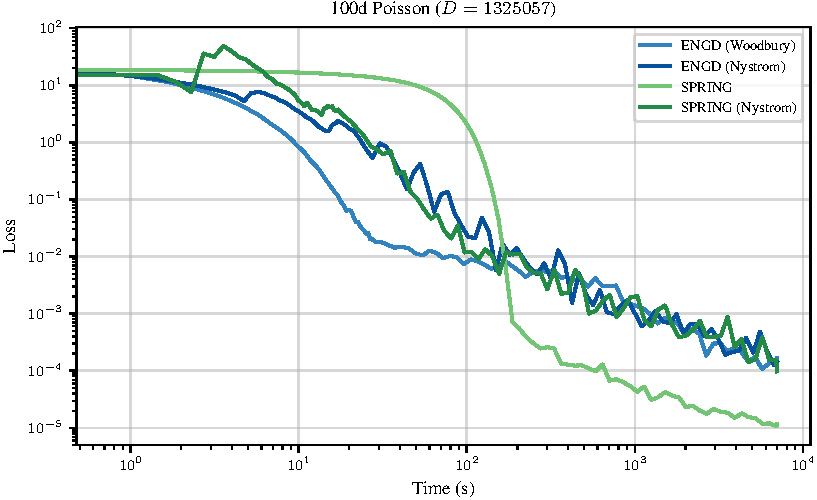
\includegraphics[trim={0 0.8cm 0 0.3cm},clip]{\pathToFigs/loss_over_time.pdf}
  \end{subfigure}
  \begin{subfigure}[t]{1.0\linewidth}
    \caption{}\label{subfig:poisson5d-step}
    % trim the legend, xlabel and xticklabels
    % [trim={left bottom right top},clip]
    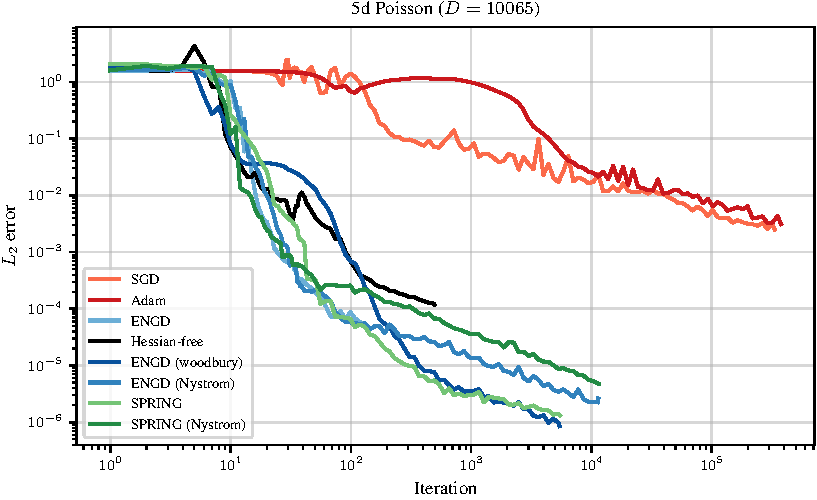
\includegraphics[trim={0 1.3cm 0 0.3cm},clip]{\pathToFigs/l2_error_over_step.pdf}
    % trim the titles
    \includegraphics[trim={0 0 0 0.3cm},clip]{\pathToFigs/loss_over_step.pdf}
  \end{subfigure}
  \caption{Training loss and evaluation $L_2$ error for learning the solution to a 5d Poisson equation over (\subref{subfig:poisson5d-time}) time and (\subref{subfig:poisson5d-step}) steps.
    Columns are different neural networks.}\label{fig:poisson5d-appendix}
\end{figure}

\paragraph{Best run details}
The runs shown in \Cref{fig:poisson5d-appendix} correspond to the following hyper-parameters:
\begin{itemize}
\item $5\to 64\to 1$ MLP with $D=449$
  \begin{itemize}
    \def\pathToRuns{kfac_pinns_exp/exp10_reproduce_poisson5d/tex}
  \item \textbf{SGD:} learning rate: $\num[scientific-notation=true]{2.686653e-04}$, momentum: $\num[scientific-notation=true]{9.878243e-01}$, $N_{\Omega}$: $\num[scientific-notation=false]{606}$, $N_{\partial\Omega}$: $\num[scientific-notation=false]{2001}$, batch sampling frequency: $\num[scientific-notation=false]{1570}$
  \item \textbf{Adam:} learning rate: $\num[scientific-notation=true]{5.416376e-04}$
  \item \textbf{Hessian-free:} curvature matrix: $\text{GGN}$, initial damping: $\num[scientific-notation=true]{0.1}$, constant damping: $\text{no}$, maximum CG iterations: $\num[scientific-notation=false]{250}$
  \item \textbf{LBFGS:} learning rate: $\num[scientific-notation=true]{0.2}$, history size: $\num[scientific-notation=false]{225}$
  \item \textbf{ENGD (full):} damping: $\num[scientific-notation=true]{1e-08}$, exponential moving average: $\num[scientific-notation=false]{0}$, initialize Gramian to identity: $\text{yes}$
  \item \textbf{ENGD (layer-wise):} damping: $\num[scientific-notation=true]{1e-06}$, exponential moving average: $\num[scientific-notation=false]{0}$, initialize Gramian to identity: $\text{yes}$
  \item \textbf{KFAC:} damping: $\num[scientific-notation=true]{3.169186e-13}$, momentum: $\num[scientific-notation=true]{7.075879e-01}$, exponential moving average: $\num[scientific-notation=true]{8.860410e-01}$, initialize Kronecker factors to identity: $\text{yes}$
  \item \textbf{KFAC*:} damping: $\num[scientific-notation=true]{2.965060e-08}$, exponential moving average: $\num[scientific-notation=true]{9.574717e-01}$, initialize Kronecker factors to identity: $\text{yes}$
  \end{itemize}

\item $5 \to 64 \to 64 \to 48 \to 48 \to 1$ MLP with $D=\num{10065}$
  \begin{itemize}
    \def\pathToRuns{kfac_pinns_exp/exp16_poisson5d_deepwide/tex}
  \item \textbf{SGD:} learning rate: $\num[scientific-notation=true]{2.686653e-04}$, momentum: $\num[scientific-notation=true]{9.878243e-01}$, $N_{\Omega}$: $\num[scientific-notation=false]{606}$, $N_{\partial\Omega}$: $\num[scientific-notation=false]{2001}$, batch sampling frequency: $\num[scientific-notation=false]{1570}$
  \item \textbf{Adam:} learning rate: $\num[scientific-notation=true]{5.416376e-04}$
  \item \textbf{Hessian-free:} curvature matrix: $\text{GGN}$, initial damping: $\num[scientific-notation=true]{0.1}$, constant damping: $\text{no}$, maximum CG iterations: $\num[scientific-notation=false]{250}$
  \item \textbf{LBFGS:} learning rate: $\num[scientific-notation=true]{0.2}$, history size: $\num[scientific-notation=false]{225}$
  \item \textbf{ENGD (full):} damping: $\num[scientific-notation=true]{1e-08}$, exponential moving average: $\num[scientific-notation=false]{0}$, initialize Gramian to identity: $\text{yes}$
  \item \textbf{ENGD (layer-wise):} damping: $\num[scientific-notation=true]{1e-06}$, exponential moving average: $\num[scientific-notation=false]{0}$, initialize Gramian to identity: $\text{yes}$
  \item \textbf{KFAC:} damping: $\num[scientific-notation=true]{3.169186e-13}$, momentum: $\num[scientific-notation=true]{7.075879e-01}$, exponential moving average: $\num[scientific-notation=true]{8.860410e-01}$, initialize Kronecker factors to identity: $\text{yes}$
  \item \textbf{KFAC*:} damping: $\num[scientific-notation=true]{2.965060e-08}$, exponential moving average: $\num[scientific-notation=true]{9.574717e-01}$, initialize Kronecker factors to identity: $\text{yes}$
  \end{itemize}

\item $5 \to 256 \to 256\to 128 \to 128 \to 1$ MLP with $D=\num{116865}$
  \begin{itemize}
    \def\pathToRuns{kfac_pinns_exp/exp19_poisson5d_mlp_tanh_256/tex}
  \item \textbf{SGD:} learning rate: $\num[scientific-notation=true]{2.686653e-04}$, momentum: $\num[scientific-notation=true]{9.878243e-01}$, $N_{\Omega}$: $\num[scientific-notation=false]{606}$, $N_{\partial\Omega}$: $\num[scientific-notation=false]{2001}$, batch sampling frequency: $\num[scientific-notation=false]{1570}$
  \item \textbf{Adam:} learning rate: $\num[scientific-notation=true]{5.416376e-04}$
  \item \textbf{Hessian-free:} curvature matrix: $\text{GGN}$, initial damping: $\num[scientific-notation=true]{0.1}$, constant damping: $\text{no}$, maximum CG iterations: $\num[scientific-notation=false]{250}$
  \item \textbf{LBFGS:} learning rate: $\num[scientific-notation=true]{0.2}$, history size: $\num[scientific-notation=false]{225}$
  \item \textbf{KFAC:} damping: $\num[scientific-notation=true]{3.169186e-13}$, momentum: $\num[scientific-notation=true]{7.075879e-01}$, exponential moving average: $\num[scientific-notation=true]{8.860410e-01}$, initialize Kronecker factors to identity: $\text{yes}$
  \item \textbf{KFAC*:} damping: $\num[scientific-notation=true]{2.965060e-08}$, exponential moving average: $\num[scientific-notation=true]{9.574717e-01}$, initialize Kronecker factors to identity: $\text{yes}$
  \end{itemize}
\end{itemize}

\paragraph{Search space details} The runs shown in \Cref{fig:poisson5d-appendix} were determined to be the best via a search with approximately 50 runs on the following search spaces which were obtained by refining an initially wider search ($\mathcal{U}$ denotes a uniform, and $\mathcal{LU}$ a log-uniform distribution):
\begin{itemize}
\item $5\to 64\to 1$ MLP with $D=449$
  \begin{itemize}
    \def\pathToRuns{kfac_pinns_exp/exp10_reproduce_poisson5d/tex}
  \item \textbf{SGD:} learning rate: $\mathcal{LU}([\num[scientific-notation=true]{1e-06}; \num[scientific-notation=false]{1}])$, momentum: $\mathcal{U}([\num[scientific-notation=false]{0}; \num[scientific-notation=true]{0.99}])$, $N_{\Omega}$: $\mathcal{U}(\{\num[scientific-notation=false]{100},\num[scientific-notation=false]{101},\text{\dots},\num[scientific-notation=false]{10000}\})$, $N_{\partial\Omega}$: $\mathcal{U}(\{\num[scientific-notation=false]{50},\num[scientific-notation=false]{51},\text{\dots},\num[scientific-notation=false]{5000}\})$, batch sampling frequency: $\mathcal{U}(\{\num[scientific-notation=false]{0},\num[scientific-notation=false]{1},\text{\dots},\num[scientific-notation=false]{10000}\})$
  \item \textbf{Adam:} learning rate: $\mathcal{LU}([\num[scientific-notation=true]{1e-06}; \num[scientific-notation=false]{1}])$, $N_{\Omega}$: $\mathcal{U}(\{\num[scientific-notation=false]{100},\num[scientific-notation=false]{101},\text{\dots},\num[scientific-notation=false]{5000}\})$, $N_{\partial\Omega}$: $\mathcal{U}(\{\num[scientific-notation=false]{50},\num[scientific-notation=false]{51},\text{\dots},\num[scientific-notation=false]{2500}\})$, batch sampling frequency: $\mathcal{U}(\{\num[scientific-notation=false]{0},\num[scientific-notation=false]{1},\text{\dots},\num[scientific-notation=false]{1000}\})$
  \item \textbf{Hessian-free:} curvature matrix: $\mathcal{U}(\{\text{GGN},\text{Hessian}\})$, initial damping: $\mathcal{LU}([\num[scientific-notation=true]{1e-15}; \num[scientific-notation=false]{1}])$, constant damping: $\mathcal{U}(\{\text{no},\text{yes}\})$, maximum CG iterations: $\mathcal{U}(\{\num[scientific-notation=false]{1},\num[scientific-notation=false]{2},\text{\dots},\num[scientific-notation=false]{500}\})$, $N_{\Omega}$: $\mathcal{U}(\{\num[scientific-notation=false]{100},\num[scientific-notation=false]{101},\text{\dots},\num[scientific-notation=false]{10000}\})$, $N_{\partial\Omega}$: $\mathcal{U}(\{\num[scientific-notation=false]{50},\num[scientific-notation=false]{51},\text{\dots},\num[scientific-notation=false]{5000}\})$, batch sampling frequency: $\mathcal{U}(\{\num[scientific-notation=false]{0},\num[scientific-notation=false]{1},\text{\dots},\num[scientific-notation=false]{10000}\})$
  \item \textbf{LBFGS:} learning rate: $\mathcal{LU}([\num[scientific-notation=true]{1e-06}; \num[scientific-notation=false]{1}])$, history size: $\mathcal{U}(\{\num[scientific-notation=false]{5},\num[scientific-notation=false]{6},\text{\dots},\num[scientific-notation=false]{500}\})$, $N_{\Omega}$: $\mathcal{U}(\{\num[scientific-notation=false]{100},\num[scientific-notation=false]{101},\text{\dots},\num[scientific-notation=false]{5000}\})$, $N_{\partial\Omega}$: $\mathcal{U}(\{\num[scientific-notation=false]{50},\num[scientific-notation=false]{51},\text{\dots},\num[scientific-notation=false]{2500}\})$, batch sampling frequency: $\mathcal{U}(\{\num[scientific-notation=false]{0},\num[scientific-notation=false]{1},\text{\dots},\num[scientific-notation=false]{5000}\})$
  \item \textbf{ENGD (full):} damping: $\mathcal{U}(\{\num[scientific-notation=true]{1e-06},\num[scientific-notation=true]{1e-08},\num[scientific-notation=true]{1e-10},\num[scientific-notation=true]{1e-12},\num[scientific-notation=false]{0}\})$, exponential moving average: $\mathcal{U}(\{\num[scientific-notation=false]{0},\num[scientific-notation=true]{0.3},\num[scientific-notation=true]{0.6},\num[scientific-notation=true]{0.9},\num[scientific-notation=true]{0.99}\})$, initialize Gramian to identity: $\mathcal{U}(\{\text{no},\text{yes}\})$
  \item \textbf{ENGD (layer-wise):} damping: $\mathcal{U}(\{\num[scientific-notation=true]{0.0001},\num[scientific-notation=true]{1e-06},\num[scientific-notation=true]{1e-08},\num[scientific-notation=true]{1e-10},\num[scientific-notation=false]{0}\})$, exponential moving average: $\mathcal{U}(\{\num[scientific-notation=false]{0},\num[scientific-notation=true]{0.3},\num[scientific-notation=true]{0.6},\num[scientific-notation=true]{0.9},\num[scientific-notation=true]{0.99}\})$, initialize Gramian to identity: $\mathcal{U}(\{\text{no},\text{yes}\})$
  \item \textbf{KFAC:} damping: $\mathcal{LU}([\num[scientific-notation=true]{1e-12}; \num[scientific-notation=true]{1e-06}])$, momentum: $\mathcal{U}([\num[scientific-notation=false]{0}; \num[scientific-notation=true]{0.99}])$, exponential moving average: $\mathcal{U}([\num[scientific-notation=true]{0.5}; \num[scientific-notation=true]{0.99}])$, initialize Kronecker factors to identity: $\text{yes}$
  \item \textbf{KFAC*:} damping: $\mathcal{LU}([\num[scientific-notation=true]{1e-15}; \num[scientific-notation=true]{1e-09}])$, exponential moving average: $\mathcal{U}([\num[scientific-notation=true]{0.5}; \num[scientific-notation=true]{0.99}])$, initialize Kronecker factors to identity: $\text{yes}$
  \end{itemize}

\item $5 \to 64 \to 64 \to 48 \to 48 \to 1$ MLP with $D=\num{10065}$
  \begin{itemize}
    \def\pathToRuns{kfac_pinns_exp/exp16_poisson5d_deepwide/tex}
  \item \textbf{SGD:} learning rate: $\mathcal{LU}([\num[scientific-notation=true]{1e-06}; \num[scientific-notation=false]{1}])$, momentum: $\mathcal{U}([\num[scientific-notation=false]{0}; \num[scientific-notation=true]{0.99}])$, $N_{\Omega}$: $\mathcal{U}(\{\num[scientific-notation=false]{100},\num[scientific-notation=false]{101},\text{\dots},\num[scientific-notation=false]{10000}\})$, $N_{\partial\Omega}$: $\mathcal{U}(\{\num[scientific-notation=false]{50},\num[scientific-notation=false]{51},\text{\dots},\num[scientific-notation=false]{5000}\})$, batch sampling frequency: $\mathcal{U}(\{\num[scientific-notation=false]{0},\num[scientific-notation=false]{1},\text{\dots},\num[scientific-notation=false]{10000}\})$
  \item \textbf{Adam:} learning rate: $\mathcal{LU}([\num[scientific-notation=true]{1e-06}; \num[scientific-notation=false]{1}])$, $N_{\Omega}$: $\mathcal{U}(\{\num[scientific-notation=false]{100},\num[scientific-notation=false]{101},\text{\dots},\num[scientific-notation=false]{5000}\})$, $N_{\partial\Omega}$: $\mathcal{U}(\{\num[scientific-notation=false]{50},\num[scientific-notation=false]{51},\text{\dots},\num[scientific-notation=false]{2500}\})$, batch sampling frequency: $\mathcal{U}(\{\num[scientific-notation=false]{0},\num[scientific-notation=false]{1},\text{\dots},\num[scientific-notation=false]{1000}\})$
  \item \textbf{Hessian-free:} curvature matrix: $\mathcal{U}(\{\text{GGN},\text{Hessian}\})$, initial damping: $\mathcal{LU}([\num[scientific-notation=true]{1e-15}; \num[scientific-notation=false]{1}])$, constant damping: $\mathcal{U}(\{\text{no},\text{yes}\})$, maximum CG iterations: $\mathcal{U}(\{\num[scientific-notation=false]{1},\num[scientific-notation=false]{2},\text{\dots},\num[scientific-notation=false]{500}\})$, $N_{\Omega}$: $\mathcal{U}(\{\num[scientific-notation=false]{100},\num[scientific-notation=false]{101},\text{\dots},\num[scientific-notation=false]{10000}\})$, $N_{\partial\Omega}$: $\mathcal{U}(\{\num[scientific-notation=false]{50},\num[scientific-notation=false]{51},\text{\dots},\num[scientific-notation=false]{5000}\})$, batch sampling frequency: $\mathcal{U}(\{\num[scientific-notation=false]{0},\num[scientific-notation=false]{1},\text{\dots},\num[scientific-notation=false]{10000}\})$
  \item \textbf{LBFGS:} learning rate: $\mathcal{LU}([\num[scientific-notation=true]{1e-06}; \num[scientific-notation=false]{1}])$, history size: $\mathcal{U}(\{\num[scientific-notation=false]{5},\num[scientific-notation=false]{6},\text{\dots},\num[scientific-notation=false]{500}\})$, $N_{\Omega}$: $\mathcal{U}(\{\num[scientific-notation=false]{100},\num[scientific-notation=false]{101},\text{\dots},\num[scientific-notation=false]{5000}\})$, $N_{\partial\Omega}$: $\mathcal{U}(\{\num[scientific-notation=false]{50},\num[scientific-notation=false]{51},\text{\dots},\num[scientific-notation=false]{2500}\})$, batch sampling frequency: $\mathcal{U}(\{\num[scientific-notation=false]{0},\num[scientific-notation=false]{1},\text{\dots},\num[scientific-notation=false]{5000}\})$
  \item \textbf{ENGD (full):} damping: $\mathcal{U}(\{\num[scientific-notation=true]{1e-06},\num[scientific-notation=true]{1e-08},\num[scientific-notation=true]{1e-10},\num[scientific-notation=true]{1e-12},\num[scientific-notation=false]{0}\})$, exponential moving average: $\mathcal{U}(\{\num[scientific-notation=false]{0},\num[scientific-notation=true]{0.3},\num[scientific-notation=true]{0.6},\num[scientific-notation=true]{0.9},\num[scientific-notation=true]{0.99}\})$, initialize Gramian to identity: $\mathcal{U}(\{\text{no},\text{yes}\})$
  \item \textbf{ENGD (layer-wise):} damping: $\mathcal{U}(\{\num[scientific-notation=true]{0.0001},\num[scientific-notation=true]{1e-06},\num[scientific-notation=true]{1e-08},\num[scientific-notation=true]{1e-10},\num[scientific-notation=false]{0}\})$, exponential moving average: $\mathcal{U}(\{\num[scientific-notation=false]{0},\num[scientific-notation=true]{0.3},\num[scientific-notation=true]{0.6},\num[scientific-notation=true]{0.9},\num[scientific-notation=true]{0.99}\})$, initialize Gramian to identity: $\mathcal{U}(\{\text{no},\text{yes}\})$
  \item \textbf{KFAC:} damping: $\mathcal{LU}([\num[scientific-notation=true]{1e-12}; \num[scientific-notation=true]{1e-06}])$, momentum: $\mathcal{U}([\num[scientific-notation=false]{0}; \num[scientific-notation=true]{0.99}])$, exponential moving average: $\mathcal{U}([\num[scientific-notation=true]{0.5}; \num[scientific-notation=true]{0.99}])$, initialize Kronecker factors to identity: $\text{yes}$
  \item \textbf{KFAC*:} damping: $\mathcal{LU}([\num[scientific-notation=true]{1e-15}; \num[scientific-notation=true]{1e-09}])$, exponential moving average: $\mathcal{U}([\num[scientific-notation=true]{0.5}; \num[scientific-notation=true]{0.99}])$, initialize Kronecker factors to identity: $\text{yes}$
  \end{itemize}

\item $5 \to 256 \to 256\to 128 \to 128 \to 1$ MLP with $D=\num{116865}$
  \begin{itemize}
    \def\pathToRuns{kfac_pinns_exp/exp19_poisson5d_mlp_tanh_256/tex}
  \item \textbf{SGD:} learning rate: $\mathcal{LU}([\num[scientific-notation=true]{1e-06}; \num[scientific-notation=false]{1}])$, momentum: $\mathcal{U}([\num[scientific-notation=false]{0}; \num[scientific-notation=true]{0.99}])$, $N_{\Omega}$: $\mathcal{U}(\{\num[scientific-notation=false]{100},\num[scientific-notation=false]{101},\text{\dots},\num[scientific-notation=false]{10000}\})$, $N_{\partial\Omega}$: $\mathcal{U}(\{\num[scientific-notation=false]{50},\num[scientific-notation=false]{51},\text{\dots},\num[scientific-notation=false]{5000}\})$, batch sampling frequency: $\mathcal{U}(\{\num[scientific-notation=false]{0},\num[scientific-notation=false]{1},\text{\dots},\num[scientific-notation=false]{10000}\})$
  \item \textbf{Adam:} learning rate: $\mathcal{LU}([\num[scientific-notation=true]{1e-06}; \num[scientific-notation=false]{1}])$, $N_{\Omega}$: $\mathcal{U}(\{\num[scientific-notation=false]{100},\num[scientific-notation=false]{101},\text{\dots},\num[scientific-notation=false]{5000}\})$, $N_{\partial\Omega}$: $\mathcal{U}(\{\num[scientific-notation=false]{50},\num[scientific-notation=false]{51},\text{\dots},\num[scientific-notation=false]{2500}\})$, batch sampling frequency: $\mathcal{U}(\{\num[scientific-notation=false]{0},\num[scientific-notation=false]{1},\text{\dots},\num[scientific-notation=false]{1000}\})$
  \item \textbf{Hessian-free:} curvature matrix: $\mathcal{U}(\{\text{GGN},\text{Hessian}\})$, initial damping: $\mathcal{LU}([\num[scientific-notation=true]{1e-15}; \num[scientific-notation=false]{1}])$, constant damping: $\mathcal{U}(\{\text{no},\text{yes}\})$, maximum CG iterations: $\mathcal{U}(\{\num[scientific-notation=false]{1},\num[scientific-notation=false]{2},\text{\dots},\num[scientific-notation=false]{500}\})$, $N_{\Omega}$: $\mathcal{U}(\{\num[scientific-notation=false]{100},\num[scientific-notation=false]{101},\text{\dots},\num[scientific-notation=false]{10000}\})$, $N_{\partial\Omega}$: $\mathcal{U}(\{\num[scientific-notation=false]{50},\num[scientific-notation=false]{51},\text{\dots},\num[scientific-notation=false]{5000}\})$, batch sampling frequency: $\mathcal{U}(\{\num[scientific-notation=false]{0},\num[scientific-notation=false]{1},\text{\dots},\num[scientific-notation=false]{10000}\})$
  \item \textbf{LBFGS:} learning rate: $\mathcal{LU}([\num[scientific-notation=true]{1e-06}; \num[scientific-notation=false]{1}])$, history size: $\mathcal{U}(\{\num[scientific-notation=false]{5},\num[scientific-notation=false]{6},\text{\dots},\num[scientific-notation=false]{500}\})$, $N_{\Omega}$: $\mathcal{U}(\{\num[scientific-notation=false]{100},\num[scientific-notation=false]{101},\text{\dots},\num[scientific-notation=false]{5000}\})$, $N_{\partial\Omega}$: $\mathcal{U}(\{\num[scientific-notation=false]{50},\num[scientific-notation=false]{51},\text{\dots},\num[scientific-notation=false]{2500}\})$, batch sampling frequency: $\mathcal{U}(\{\num[scientific-notation=false]{0},\num[scientific-notation=false]{1},\text{\dots},\num[scientific-notation=false]{5000}\})$
  \item \textbf{KFAC:} damping: $\mathcal{LU}([\num[scientific-notation=true]{1e-12}; \num[scientific-notation=true]{1e-06}])$, momentum: $\mathcal{U}([\num[scientific-notation=false]{0}; \num[scientific-notation=true]{0.99}])$, exponential moving average: $\mathcal{U}([\num[scientific-notation=true]{0.5}; \num[scientific-notation=true]{0.99}])$, initialize Kronecker factors to identity: $\text{yes}$
  \item \textbf{KFAC*:} damping: $\mathcal{LU}([\num[scientific-notation=true]{1e-15}; \num[scientific-notation=true]{1e-09}])$, exponential moving average: $\mathcal{U}([\num[scientific-notation=true]{0.5}; \num[scientific-notation=true]{0.99}])$, initialize Kronecker factors to identity: $\text{yes}$
  \end{itemize}
\end{itemize}

\subsection{10d Poisson Equation}\label{sec:poisson10d-appendix}

\paragraph{Setup} We consider a 10-dimensional Poisson equation $-\Delta u(\vx) = 0$ on the 10-dimensional unit square $\vx \in [0, 1]^5$ with zero right-hand side and harmonic mixed second order polynomial boundary conditions $u(\vx) = \sum_{i=1}^{\nicefrac{d}{2}} \evx_{2i-1} \evx_{2i}$ for $\vx \in \partial [0,1]^d$.
We sample training batches of size $N_{\Omega} = \num{3000}, N_{\partial\Omega} = 1000$ and evaluate the $L_2$ error on a separate set of $\num{30000}$ data points using the known solution $u_{\star}(\vx) = \sum_{i=1}^{\nicefrac{d}{2}} \evx_{2i-1} \evx_{2i}$.
All optimizers except for KFAC sample a new training batch each iteration.
KFAC only re-samples every 100 iterations because we noticed significant improvement with multiple iterations on a fixed batch.
Each run is limited to $\num{6000}\,\text{s}$.
We use a $10 \to 256 \to 256\to 128 \to 128 \to 1$ MLP with $D=\num{118145}$ MLP whose linear layers are Tanh-activated except for the final one.
\Cref{fig:poisson_10d-appendix} visualizes the results.

\begin{figure}[!h]
  \centering
  \def\pathToFigs{kfac_pinns_exp/exp21_poisson_10d}
  \begin{subfigure}[t]{1.0\linewidth}
    \caption{}\label{subfig:poisson_10d-time}
    \includegraphics{\pathToFigs/l2_error_over_time.pdf}
    \includegraphics{\pathToFigs/loss_over_time.pdf}
  \end{subfigure}
  \begin{subfigure}[t]{1.0\linewidth}
    \caption{}\label{subfig:poisson_10d-step}
    \includegraphics{\pathToFigs/l2_error_over_step.pdf}
    \includegraphics{\pathToFigs/loss_over_step.pdf}
  \end{subfigure}
  \caption{Training loss and evaluation $L_2$ error for learning the solution to a 10d Poisson equation over (\subref{subfig:poisson_10d-time}) time and (\subref{subfig:poisson_10d-step}) steps.}\label{fig:poisson_10d-appendix}
\end{figure}

\paragraph{Best run details}
The runs shown in \Cref{fig:poisson_10d-appendix} correspond to the following hyper-parameters:
\begin{itemize}
  \def\pathToRuns{kfac_pinns_exp/exp21_poisson_10d/tex/}
\item \textbf{SGD:} learning rate: $\num[scientific-notation=true]{2.686653e-04}$, momentum: $\num[scientific-notation=true]{9.878243e-01}$, $N_{\Omega}$: $\num[scientific-notation=false]{606}$, $N_{\partial\Omega}$: $\num[scientific-notation=false]{2001}$, batch sampling frequency: $\num[scientific-notation=false]{1570}$
\item \textbf{Adam:} learning rate: $\num[scientific-notation=true]{5.416376e-04}$
\item \textbf{Hessian-free:} curvature matrix: $\text{GGN}$, initial damping: $\num[scientific-notation=true]{0.1}$, constant damping: $\text{no}$, maximum CG iterations: $\num[scientific-notation=false]{250}$
\item \textbf{LBFGS:} learning rate: $\num[scientific-notation=true]{0.2}$, history size: $\num[scientific-notation=false]{225}$
\item \textbf{KFAC:} damping: $\num[scientific-notation=true]{3.169186e-13}$, momentum: $\num[scientific-notation=true]{7.075879e-01}$, exponential moving average: $\num[scientific-notation=true]{8.860410e-01}$, initialize Kronecker factors to identity: $\text{yes}$
\item \textbf{KFAC*:} damping: $\num[scientific-notation=true]{2.965060e-08}$, exponential moving average: $\num[scientific-notation=true]{9.574717e-01}$, initialize Kronecker factors to identity: $\text{yes}$
\end{itemize}

\paragraph{Search space details} The runs shown in \Cref{fig:poisson_10d-appendix} were determined to be the best via a Bayesian search on the following search spaces which each optimizer given approximately the same total computational time ($\mathcal{U}$ denotes a uniform, and $\mathcal{LU}$ a log-uniform distribution):
\begin{itemize}
  \def\pathToRuns{kfac_pinns_exp/exp21_poisson_10d/tex/}
\item \textbf{SGD:} learning rate: $\mathcal{LU}([\num[scientific-notation=true]{1e-06}; \num[scientific-notation=false]{1}])$, momentum: $\mathcal{U}([\num[scientific-notation=false]{0}; \num[scientific-notation=true]{0.99}])$, $N_{\Omega}$: $\mathcal{U}(\{\num[scientific-notation=false]{100},\num[scientific-notation=false]{101},\text{\dots},\num[scientific-notation=false]{10000}\})$, $N_{\partial\Omega}$: $\mathcal{U}(\{\num[scientific-notation=false]{50},\num[scientific-notation=false]{51},\text{\dots},\num[scientific-notation=false]{5000}\})$, batch sampling frequency: $\mathcal{U}(\{\num[scientific-notation=false]{0},\num[scientific-notation=false]{1},\text{\dots},\num[scientific-notation=false]{10000}\})$
\item \textbf{Adam:} learning rate: $\mathcal{LU}([\num[scientific-notation=true]{1e-06}; \num[scientific-notation=false]{1}])$, $N_{\Omega}$: $\mathcal{U}(\{\num[scientific-notation=false]{100},\num[scientific-notation=false]{101},\text{\dots},\num[scientific-notation=false]{5000}\})$, $N_{\partial\Omega}$: $\mathcal{U}(\{\num[scientific-notation=false]{50},\num[scientific-notation=false]{51},\text{\dots},\num[scientific-notation=false]{2500}\})$, batch sampling frequency: $\mathcal{U}(\{\num[scientific-notation=false]{0},\num[scientific-notation=false]{1},\text{\dots},\num[scientific-notation=false]{1000}\})$
\item \textbf{Hessian-free:} curvature matrix: $\mathcal{U}(\{\text{GGN},\text{Hessian}\})$, initial damping: $\mathcal{LU}([\num[scientific-notation=true]{1e-15}; \num[scientific-notation=false]{1}])$, constant damping: $\mathcal{U}(\{\text{no},\text{yes}\})$, maximum CG iterations: $\mathcal{U}(\{\num[scientific-notation=false]{1},\num[scientific-notation=false]{2},\text{\dots},\num[scientific-notation=false]{500}\})$, $N_{\Omega}$: $\mathcal{U}(\{\num[scientific-notation=false]{100},\num[scientific-notation=false]{101},\text{\dots},\num[scientific-notation=false]{10000}\})$, $N_{\partial\Omega}$: $\mathcal{U}(\{\num[scientific-notation=false]{50},\num[scientific-notation=false]{51},\text{\dots},\num[scientific-notation=false]{5000}\})$, batch sampling frequency: $\mathcal{U}(\{\num[scientific-notation=false]{0},\num[scientific-notation=false]{1},\text{\dots},\num[scientific-notation=false]{10000}\})$
\item \textbf{LBFGS:} learning rate: $\mathcal{LU}([\num[scientific-notation=true]{1e-06}; \num[scientific-notation=false]{1}])$, history size: $\mathcal{U}(\{\num[scientific-notation=false]{5},\num[scientific-notation=false]{6},\text{\dots},\num[scientific-notation=false]{500}\})$, $N_{\Omega}$: $\mathcal{U}(\{\num[scientific-notation=false]{100},\num[scientific-notation=false]{101},\text{\dots},\num[scientific-notation=false]{5000}\})$, $N_{\partial\Omega}$: $\mathcal{U}(\{\num[scientific-notation=false]{50},\num[scientific-notation=false]{51},\text{\dots},\num[scientific-notation=false]{2500}\})$, batch sampling frequency: $\mathcal{U}(\{\num[scientific-notation=false]{0},\num[scientific-notation=false]{1},\text{\dots},\num[scientific-notation=false]{5000}\})$
\item \textbf{KFAC:} damping: $\mathcal{LU}([\num[scientific-notation=true]{1e-12}; \num[scientific-notation=true]{1e-06}])$, momentum: $\mathcal{U}([\num[scientific-notation=false]{0}; \num[scientific-notation=true]{0.99}])$, exponential moving average: $\mathcal{U}([\num[scientific-notation=true]{0.5}; \num[scientific-notation=true]{0.99}])$, initialize Kronecker factors to identity: $\text{yes}$
\item \textbf{KFAC*:} damping: $\mathcal{LU}([\num[scientific-notation=true]{1e-15}; \num[scientific-notation=true]{1e-09}])$, exponential moving average: $\mathcal{U}([\num[scientific-notation=true]{0.5}; \num[scientific-notation=true]{0.99}])$, initialize Kronecker factors to identity: $\text{yes}$
\end{itemize}

\subsection{5/10/100-d Poisson Equations with Bayesian Search}\label{sec:high-dimensional-poissons-app}

\paragraph{Setup} Here, we consider three Poisson equations $- \Delta u(\vx) = f(\vx)$ with different right-hand sides and boundary conditions on the unit square $\vx \in [0, 1]^d$:
\begin{itemize}
\item $d=5$ with cosine sum right-hand side $f(\vx) = \pi^2 \sum_{i=1}^d \cos(\pi \evx_i)$, boundary conditions $u(\vx) = \sum_{i=1}^d \cos(\pi \evx_i)$ for $\vx \in \partial [0,1]^d$, and known solution $u_{\star}(\vx) = \sum_{i=1}^d \cos(\pi \evx_i)$.
  We assign each run a budget of $\num{3000}\,\text{s}$.

\item $d=10$ with zero right-hand side $f(\vx) = 0$, harmonic mixed second order polynomial boundary conditions $u(\vx) = \sum_{i=1}^{\nicefrac{d}{2}} \evx_{2i-1} \evx_{2i}$ for $\vx \in \partial [0,1]^d$, and known solution $u_{\star}(\vx) =  \sum_{i=1}^{\nicefrac{d}{2}} \evx_{2i-1} \evx_{2i}$.
  We assign each run a budget of $\num{6000}\,\text{s}$.

\item $d=100$ with constant non-zero right-hand side $f(\vx) = -2 d$, square norm boundary conditions $u(\vx) = \left\lVert \vx \right\rVert_2^2$ for $\vx \in \partial [0,1]^d$, and known solution $u_{\star}(\vx) =  \left\lVert \vx \right\rVert_2^2$.
  We assign each run a budget of $\num{10000}\,\text{s}$.
\end{itemize}
We tune the optimizer-hyperparameters described in \Cref{sec:tuning-protocol}, as well as the batch sizes $N_{\Omega}, N_{\partial \Omega}$, and their associated re-sampling frequencies using Bayesian search.
We use five layer MLP architectures with varying widths whose layers are Tanh-activated except for the final layer.
These architectures are too large to be optimized by ENGD.
\Cref{fig:poisson-bayes-appendix} visualizes the results.

\begin{figure}[!h]
  \centering
  \def\pathToFigs{kfac_pinns_exp/exp33_poisson_bayes_groupplot}
  \begin{subfigure}[t]{1.0\linewidth}
    \caption{}\label{subfig:poisson-bayes-time}
    % trim legend, xlabel and xticklabels
    % [trim={left bottom right top},clip]
    \includegraphics[trim={0 1.3cm 0 0},clip]{\pathToFigs/l2_error_over_time.pdf}
    % trim the legend and titles
    % [trim={left bottom right top},clip]
    \includegraphics[trim={0 0.8cm 0 0.3cm},clip]{\pathToFigs/loss_over_time.pdf}
  \end{subfigure}
  \begin{subfigure}[t]{1.0\linewidth}
    \caption{}\label{subfig:poisson-bayes-step}
    % trim the legend, xlabel and xticklabels
    % [trim={left bottom right top},clip]
    \includegraphics[trim={0 1.3cm 0 0.3cm},clip]{\pathToFigs/l2_error_over_step.pdf}
    % trim the titles
    \includegraphics[trim={0 0 0 0.3cm},clip]{\pathToFigs/loss_over_step.pdf}
  \end{subfigure}
  \caption{Training loss and evaluation $L_2$ error for learning the solution to high-dimensional Poisson equations over (\subref{subfig:poisson-bayes-time}) time and (\subref{subfig:poisson-bayes-step}) steps using Bayesian search.}\label{fig:poisson-bayes-appendix}
\end{figure}

\paragraph{Best run details} The runs shown in \Cref{fig:poisson-bayes-appendix} correspond to the following hyper-parameters:

\begin{itemize}

\item 5d Poisson equation, $5 \to 256 \to 256 \to 128 \to 128 \to 1$ MLP with $D=\num{116865}$
  \begin{itemize}
    \def\pathToRuns{kfac_pinns_exp/exp26_poisson5d_mlp_tanh_256_bayes/tex}
  \item \textbf{SGD:} learning rate: $\num[scientific-notation=true]{2.686653e-04}$, momentum: $\num[scientific-notation=true]{9.878243e-01}$, $N_{\Omega}$: $\num[scientific-notation=false]{606}$, $N_{\partial\Omega}$: $\num[scientific-notation=false]{2001}$, batch sampling frequency: $\num[scientific-notation=false]{1570}$
  \item \textbf{Adam:} learning rate: $\num[scientific-notation=true]{5.416376e-04}$
  \item \textbf{Hessian-free:} curvature matrix: $\text{GGN}$, initial damping: $\num[scientific-notation=true]{0.1}$, constant damping: $\text{no}$, maximum CG iterations: $\num[scientific-notation=false]{250}$
  \item \textbf{LBFGS:} learning rate: $\num[scientific-notation=true]{0.2}$, history size: $\num[scientific-notation=false]{225}$
  \item \textbf{KFAC:} damping: $\num[scientific-notation=true]{3.169186e-13}$, momentum: $\num[scientific-notation=true]{7.075879e-01}$, exponential moving average: $\num[scientific-notation=true]{8.860410e-01}$, initialize Kronecker factors to identity: $\text{yes}$
  \item \textbf{KFAC*:} damping: $\num[scientific-notation=true]{2.965060e-08}$, exponential moving average: $\num[scientific-notation=true]{9.574717e-01}$, initialize Kronecker factors to identity: $\text{yes}$
  \end{itemize}

\item 10d Poisson equation, $10 \to 256 \to 256 \to 128 \to 128 \to 1$ MLP with $D=\num{118145}$
  \begin{itemize}
    \def\pathToRuns{kfac_pinns_exp/exp32_poisson10d_mlp_tanh_256_bayes/tex}
  \item \textbf{SGD:} learning rate: $\num[scientific-notation=true]{2.686653e-04}$, momentum: $\num[scientific-notation=true]{9.878243e-01}$, $N_{\Omega}$: $\num[scientific-notation=false]{606}$, $N_{\partial\Omega}$: $\num[scientific-notation=false]{2001}$, batch sampling frequency: $\num[scientific-notation=false]{1570}$
  \item \textbf{Adam:} learning rate: $\num[scientific-notation=true]{5.416376e-04}$
  \item \textbf{Hessian-free:} curvature matrix: $\text{GGN}$, initial damping: $\num[scientific-notation=true]{0.1}$, constant damping: $\text{no}$, maximum CG iterations: $\num[scientific-notation=false]{250}$
  \item \textbf{LBFGS:} learning rate: $\num[scientific-notation=true]{0.2}$, history size: $\num[scientific-notation=false]{225}$
  \item \textbf{KFAC:} damping: $\num[scientific-notation=true]{3.169186e-13}$, momentum: $\num[scientific-notation=true]{7.075879e-01}$, exponential moving average: $\num[scientific-notation=true]{8.860410e-01}$, initialize Kronecker factors to identity: $\text{yes}$
  \item \textbf{KFAC*:} damping: $\num[scientific-notation=true]{2.965060e-08}$, exponential moving average: $\num[scientific-notation=true]{9.574717e-01}$, initialize Kronecker factors to identity: $\text{yes}$
  \end{itemize}

\item 100d Poisson equation, $100 \to 768 \to 768 \to 512 \to 512 \to 1$ MLP with $D=\num{1325057}$
  \begin{itemize}
    \def\pathToRuns{kfac_pinns_exp/exp14_poisson_100d_weinan/tex}
  \item \textbf{SGD:} learning rate: $\num[scientific-notation=true]{2.686653e-04}$, momentum: $\num[scientific-notation=true]{9.878243e-01}$, $N_{\Omega}$: $\num[scientific-notation=false]{606}$, $N_{\partial\Omega}$: $\num[scientific-notation=false]{2001}$, batch sampling frequency: $\num[scientific-notation=false]{1570}$
  \item \textbf{Adam:} learning rate: $\num[scientific-notation=true]{5.416376e-04}$
  \item \textbf{Hessian-free:} curvature matrix: $\text{GGN}$, initial damping: $\num[scientific-notation=true]{0.1}$, constant damping: $\text{no}$, maximum CG iterations: $\num[scientific-notation=false]{250}$
  \item \textbf{LBFGS:} learning rate: $\num[scientific-notation=true]{0.2}$, history size: $\num[scientific-notation=false]{225}$
  \item \textbf{KFAC:} damping: $\num[scientific-notation=true]{3.169186e-13}$, momentum: $\num[scientific-notation=true]{7.075879e-01}$, exponential moving average: $\num[scientific-notation=true]{8.860410e-01}$, initialize Kronecker factors to identity: $\text{yes}$
  \item \textbf{KFAC*:} damping: $\num[scientific-notation=true]{2.965060e-08}$, exponential moving average: $\num[scientific-notation=true]{9.574717e-01}$, initialize Kronecker factors to identity: $\text{yes}$
  \end{itemize}
\end{itemize}

\paragraph{Search space details} The runs shown in \Cref{fig:poisson-bayes-appendix} were determined to be the best via a Bayesian search on the following search spaces which each optimizer given approximately the same total computational time ($\mathcal{U}$ denotes a uniform, and $\mathcal{LU}$ a log-uniform distribution):
\begin{itemize}

\item 5d Poisson equation, $5 \to 256 \to 256 \to 128 \to 128 \to 1$ MLP with $D=\num{116865}$
  \begin{itemize}
    \def\pathToRuns{kfac_pinns_exp/exp26_poisson5d_mlp_tanh_256_bayes/tex}
  \item \textbf{SGD:} learning rate: $\mathcal{LU}([\num[scientific-notation=true]{1e-06}; \num[scientific-notation=false]{1}])$, momentum: $\mathcal{U}([\num[scientific-notation=false]{0}; \num[scientific-notation=true]{0.99}])$, $N_{\Omega}$: $\mathcal{U}(\{\num[scientific-notation=false]{100},\num[scientific-notation=false]{101},\text{\dots},\num[scientific-notation=false]{10000}\})$, $N_{\partial\Omega}$: $\mathcal{U}(\{\num[scientific-notation=false]{50},\num[scientific-notation=false]{51},\text{\dots},\num[scientific-notation=false]{5000}\})$, batch sampling frequency: $\mathcal{U}(\{\num[scientific-notation=false]{0},\num[scientific-notation=false]{1},\text{\dots},\num[scientific-notation=false]{10000}\})$
  \item \textbf{Adam:} learning rate: $\mathcal{LU}([\num[scientific-notation=true]{1e-06}; \num[scientific-notation=false]{1}])$, $N_{\Omega}$: $\mathcal{U}(\{\num[scientific-notation=false]{100},\num[scientific-notation=false]{101},\text{\dots},\num[scientific-notation=false]{5000}\})$, $N_{\partial\Omega}$: $\mathcal{U}(\{\num[scientific-notation=false]{50},\num[scientific-notation=false]{51},\text{\dots},\num[scientific-notation=false]{2500}\})$, batch sampling frequency: $\mathcal{U}(\{\num[scientific-notation=false]{0},\num[scientific-notation=false]{1},\text{\dots},\num[scientific-notation=false]{1000}\})$
  \item \textbf{Hessian-free:} curvature matrix: $\mathcal{U}(\{\text{GGN},\text{Hessian}\})$, initial damping: $\mathcal{LU}([\num[scientific-notation=true]{1e-15}; \num[scientific-notation=false]{1}])$, constant damping: $\mathcal{U}(\{\text{no},\text{yes}\})$, maximum CG iterations: $\mathcal{U}(\{\num[scientific-notation=false]{1},\num[scientific-notation=false]{2},\text{\dots},\num[scientific-notation=false]{500}\})$, $N_{\Omega}$: $\mathcal{U}(\{\num[scientific-notation=false]{100},\num[scientific-notation=false]{101},\text{\dots},\num[scientific-notation=false]{10000}\})$, $N_{\partial\Omega}$: $\mathcal{U}(\{\num[scientific-notation=false]{50},\num[scientific-notation=false]{51},\text{\dots},\num[scientific-notation=false]{5000}\})$, batch sampling frequency: $\mathcal{U}(\{\num[scientific-notation=false]{0},\num[scientific-notation=false]{1},\text{\dots},\num[scientific-notation=false]{10000}\})$
  \item \textbf{LBFGS:} learning rate: $\mathcal{LU}([\num[scientific-notation=true]{1e-06}; \num[scientific-notation=false]{1}])$, history size: $\mathcal{U}(\{\num[scientific-notation=false]{5},\num[scientific-notation=false]{6},\text{\dots},\num[scientific-notation=false]{500}\})$, $N_{\Omega}$: $\mathcal{U}(\{\num[scientific-notation=false]{100},\num[scientific-notation=false]{101},\text{\dots},\num[scientific-notation=false]{5000}\})$, $N_{\partial\Omega}$: $\mathcal{U}(\{\num[scientific-notation=false]{50},\num[scientific-notation=false]{51},\text{\dots},\num[scientific-notation=false]{2500}\})$, batch sampling frequency: $\mathcal{U}(\{\num[scientific-notation=false]{0},\num[scientific-notation=false]{1},\text{\dots},\num[scientific-notation=false]{5000}\})$
  \item \textbf{KFAC:} damping: $\mathcal{LU}([\num[scientific-notation=true]{1e-12}; \num[scientific-notation=true]{1e-06}])$, momentum: $\mathcal{U}([\num[scientific-notation=false]{0}; \num[scientific-notation=true]{0.99}])$, exponential moving average: $\mathcal{U}([\num[scientific-notation=true]{0.5}; \num[scientific-notation=true]{0.99}])$, initialize Kronecker factors to identity: $\text{yes}$
  \item \textbf{KFAC*:} damping: $\mathcal{LU}([\num[scientific-notation=true]{1e-15}; \num[scientific-notation=true]{1e-09}])$, exponential moving average: $\mathcal{U}([\num[scientific-notation=true]{0.5}; \num[scientific-notation=true]{0.99}])$, initialize Kronecker factors to identity: $\text{yes}$
  \end{itemize}

\item 10d Poisson equation, $10 \to 256 \to 256 \to 128 \to 128 \to 1$ MLP with $D=\num{118145}$
  \begin{itemize}
    \def\pathToRuns{kfac_pinns_exp/exp32_poisson10d_mlp_tanh_256_bayes/tex}
  \item \textbf{SGD:} learning rate: $\mathcal{LU}([\num[scientific-notation=true]{1e-06}; \num[scientific-notation=false]{1}])$, momentum: $\mathcal{U}([\num[scientific-notation=false]{0}; \num[scientific-notation=true]{0.99}])$, $N_{\Omega}$: $\mathcal{U}(\{\num[scientific-notation=false]{100},\num[scientific-notation=false]{101},\text{\dots},\num[scientific-notation=false]{10000}\})$, $N_{\partial\Omega}$: $\mathcal{U}(\{\num[scientific-notation=false]{50},\num[scientific-notation=false]{51},\text{\dots},\num[scientific-notation=false]{5000}\})$, batch sampling frequency: $\mathcal{U}(\{\num[scientific-notation=false]{0},\num[scientific-notation=false]{1},\text{\dots},\num[scientific-notation=false]{10000}\})$
  \item \textbf{Adam:} learning rate: $\mathcal{LU}([\num[scientific-notation=true]{1e-06}; \num[scientific-notation=false]{1}])$, $N_{\Omega}$: $\mathcal{U}(\{\num[scientific-notation=false]{100},\num[scientific-notation=false]{101},\text{\dots},\num[scientific-notation=false]{5000}\})$, $N_{\partial\Omega}$: $\mathcal{U}(\{\num[scientific-notation=false]{50},\num[scientific-notation=false]{51},\text{\dots},\num[scientific-notation=false]{2500}\})$, batch sampling frequency: $\mathcal{U}(\{\num[scientific-notation=false]{0},\num[scientific-notation=false]{1},\text{\dots},\num[scientific-notation=false]{1000}\})$
  \item \textbf{Hessian-free:} curvature matrix: $\mathcal{U}(\{\text{GGN},\text{Hessian}\})$, initial damping: $\mathcal{LU}([\num[scientific-notation=true]{1e-15}; \num[scientific-notation=false]{1}])$, constant damping: $\mathcal{U}(\{\text{no},\text{yes}\})$, maximum CG iterations: $\mathcal{U}(\{\num[scientific-notation=false]{1},\num[scientific-notation=false]{2},\text{\dots},\num[scientific-notation=false]{500}\})$, $N_{\Omega}$: $\mathcal{U}(\{\num[scientific-notation=false]{100},\num[scientific-notation=false]{101},\text{\dots},\num[scientific-notation=false]{10000}\})$, $N_{\partial\Omega}$: $\mathcal{U}(\{\num[scientific-notation=false]{50},\num[scientific-notation=false]{51},\text{\dots},\num[scientific-notation=false]{5000}\})$, batch sampling frequency: $\mathcal{U}(\{\num[scientific-notation=false]{0},\num[scientific-notation=false]{1},\text{\dots},\num[scientific-notation=false]{10000}\})$
  \item \textbf{LBFGS:} learning rate: $\mathcal{LU}([\num[scientific-notation=true]{1e-06}; \num[scientific-notation=false]{1}])$, history size: $\mathcal{U}(\{\num[scientific-notation=false]{5},\num[scientific-notation=false]{6},\text{\dots},\num[scientific-notation=false]{500}\})$, $N_{\Omega}$: $\mathcal{U}(\{\num[scientific-notation=false]{100},\num[scientific-notation=false]{101},\text{\dots},\num[scientific-notation=false]{5000}\})$, $N_{\partial\Omega}$: $\mathcal{U}(\{\num[scientific-notation=false]{50},\num[scientific-notation=false]{51},\text{\dots},\num[scientific-notation=false]{2500}\})$, batch sampling frequency: $\mathcal{U}(\{\num[scientific-notation=false]{0},\num[scientific-notation=false]{1},\text{\dots},\num[scientific-notation=false]{5000}\})$
  \item \textbf{KFAC:} damping: $\mathcal{LU}([\num[scientific-notation=true]{1e-12}; \num[scientific-notation=true]{1e-06}])$, momentum: $\mathcal{U}([\num[scientific-notation=false]{0}; \num[scientific-notation=true]{0.99}])$, exponential moving average: $\mathcal{U}([\num[scientific-notation=true]{0.5}; \num[scientific-notation=true]{0.99}])$, initialize Kronecker factors to identity: $\text{yes}$
  \item \textbf{KFAC*:} damping: $\mathcal{LU}([\num[scientific-notation=true]{1e-15}; \num[scientific-notation=true]{1e-09}])$, exponential moving average: $\mathcal{U}([\num[scientific-notation=true]{0.5}; \num[scientific-notation=true]{0.99}])$, initialize Kronecker factors to identity: $\text{yes}$
  \end{itemize}

\item 100d Poisson equation, $100 \to 768 \to 768 \to 512 \to 512 \to 1$ MLP with $D=\num{1325057}$
  \begin{itemize}
    \def\pathToRuns{kfac_pinns_exp/exp14_poisson_100d_weinan/tex}
  \item \textbf{SGD:} learning rate: $\mathcal{LU}([\num[scientific-notation=true]{1e-06}; \num[scientific-notation=false]{1}])$, momentum: $\mathcal{U}([\num[scientific-notation=false]{0}; \num[scientific-notation=true]{0.99}])$, $N_{\Omega}$: $\mathcal{U}(\{\num[scientific-notation=false]{100},\num[scientific-notation=false]{101},\text{\dots},\num[scientific-notation=false]{10000}\})$, $N_{\partial\Omega}$: $\mathcal{U}(\{\num[scientific-notation=false]{50},\num[scientific-notation=false]{51},\text{\dots},\num[scientific-notation=false]{5000}\})$, batch sampling frequency: $\mathcal{U}(\{\num[scientific-notation=false]{0},\num[scientific-notation=false]{1},\text{\dots},\num[scientific-notation=false]{10000}\})$
  \item \textbf{Adam:} learning rate: $\mathcal{LU}([\num[scientific-notation=true]{1e-06}; \num[scientific-notation=false]{1}])$, $N_{\Omega}$: $\mathcal{U}(\{\num[scientific-notation=false]{100},\num[scientific-notation=false]{101},\text{\dots},\num[scientific-notation=false]{5000}\})$, $N_{\partial\Omega}$: $\mathcal{U}(\{\num[scientific-notation=false]{50},\num[scientific-notation=false]{51},\text{\dots},\num[scientific-notation=false]{2500}\})$, batch sampling frequency: $\mathcal{U}(\{\num[scientific-notation=false]{0},\num[scientific-notation=false]{1},\text{\dots},\num[scientific-notation=false]{1000}\})$
  \item \textbf{Hessian-free:} curvature matrix: $\mathcal{U}(\{\text{GGN},\text{Hessian}\})$, initial damping: $\mathcal{LU}([\num[scientific-notation=true]{1e-15}; \num[scientific-notation=false]{1}])$, constant damping: $\mathcal{U}(\{\text{no},\text{yes}\})$, maximum CG iterations: $\mathcal{U}(\{\num[scientific-notation=false]{1},\num[scientific-notation=false]{2},\text{\dots},\num[scientific-notation=false]{500}\})$, $N_{\Omega}$: $\mathcal{U}(\{\num[scientific-notation=false]{100},\num[scientific-notation=false]{101},\text{\dots},\num[scientific-notation=false]{10000}\})$, $N_{\partial\Omega}$: $\mathcal{U}(\{\num[scientific-notation=false]{50},\num[scientific-notation=false]{51},\text{\dots},\num[scientific-notation=false]{5000}\})$, batch sampling frequency: $\mathcal{U}(\{\num[scientific-notation=false]{0},\num[scientific-notation=false]{1},\text{\dots},\num[scientific-notation=false]{10000}\})$
  \item \textbf{LBFGS:} learning rate: $\mathcal{LU}([\num[scientific-notation=true]{1e-06}; \num[scientific-notation=false]{1}])$, history size: $\mathcal{U}(\{\num[scientific-notation=false]{5},\num[scientific-notation=false]{6},\text{\dots},\num[scientific-notation=false]{500}\})$, $N_{\Omega}$: $\mathcal{U}(\{\num[scientific-notation=false]{100},\num[scientific-notation=false]{101},\text{\dots},\num[scientific-notation=false]{5000}\})$, $N_{\partial\Omega}$: $\mathcal{U}(\{\num[scientific-notation=false]{50},\num[scientific-notation=false]{51},\text{\dots},\num[scientific-notation=false]{2500}\})$, batch sampling frequency: $\mathcal{U}(\{\num[scientific-notation=false]{0},\num[scientific-notation=false]{1},\text{\dots},\num[scientific-notation=false]{5000}\})$
  \item \textbf{KFAC:} damping: $\mathcal{LU}([\num[scientific-notation=true]{1e-12}; \num[scientific-notation=true]{1e-06}])$, momentum: $\mathcal{U}([\num[scientific-notation=false]{0}; \num[scientific-notation=true]{0.99}])$, exponential moving average: $\mathcal{U}([\num[scientific-notation=true]{0.5}; \num[scientific-notation=true]{0.99}])$, initialize Kronecker factors to identity: $\text{yes}$
  \item \textbf{KFAC*:} damping: $\mathcal{LU}([\num[scientific-notation=true]{1e-15}; \num[scientific-notation=true]{1e-09}])$, exponential moving average: $\mathcal{U}([\num[scientific-notation=true]{0.5}; \num[scientific-notation=true]{0.99}])$, initialize Kronecker factors to identity: $\text{yes}$
  \end{itemize}
\end{itemize}

\subsection{PINN Loss for the Heat Equation}\label{sec:pinn-loss-heat-equation}
Consider the $(\tilde{d}+1)$-dimensional homogeneous heat equation
\begin{align*}
  \partial_{t} u(t, \tilde{\vx})
  -
  \kappa \Delta_{\tilde{\vx}} u(t, \tilde{\vx})
  =
  0
\end{align*}
with spatial coordinates $\tilde{\vx} \in \Omega \subseteq \sR^{\tilde{d}}$ and time coordinate $t \in \mathrm{T} \subseteq \sR$ where $\mathrm{T}$ is a time interval and $\kappa >0$ denotes the heat conductivity. In this case, our neural network processes a $(d = \tilde{d} +1)$-dimensional vector $\vx = ( t,  \tilde{\vx}^{\top} )^{\top} \in \sR^d$ and we can re-write the heat equation as
\begin{align*}
  \partial_{\evx_1} u(\vx)
  -
  \kappa \sum_{d=2}^{d} \Delta_{\evx_d} u(\vx)
  =
  0\,.
\end{align*}
In the following, we consider the unit time interval $\mathrm{T} = [0;1]$, the unit square $\Omega = [0;1]^{\tilde{d}}$ and set $\kappa = \nicefrac{1}{4}$.
There are two types of constraints we need to enforce on the heat equation in order to obtain unique solutions: initial conditions and boundary conditions.
As our framework for the KFAC approximation assumes only two terms in the loss function, we combine the contributions from the boundary and initial values into one term.

To make this more precise, consider the following example solution of the heat equation, which will be used later on as well.
As initial conditions, we use $u_0(\tilde{\vx}) = u(0, \tilde{\vx}) = \prod_{i=1}^{\tilde{d}} \sin(\pi \tilde{\evx}_i)$ for $\tilde{\vx} \in \Omega$.
For boundary conditions, we use $g(t, \tilde{\vx}) = 0$ for $(t, \tilde{\vx}) \in \mathrm{T} \times \partial\Omega$.
The manufactured solution is
\begin{align*}
  u_{\star}(t, \tilde{\vx})
  =
  \exp \left(-\frac{\pi^2 \tilde{d} t}{4} \right)
  \prod_{i=1}^{\tilde{d}} \sin(\pi [\tilde{\evx}_i])\,.
\end{align*}
The PINN loss for this problem consists of three terms: a PDE term, an initial value condition term, and a spatial boundary condition term,
\begin{align*}
  L(\vtheta)
  &=
    \frac{1}{N_{\Omega}}
    \sum_{n=1}^{N_{\Omega}}
    \left(
    \partial_t u_{\vtheta}(\vx_n^{\Omega})
    -
    \frac{1}{4} \Delta_{\tilde{\vx}_n} u_{\vtheta}(\vx_n^{\Omega})
    \right)^2
  \\
  &+
    \frac{1}{N_{\partial\Omega}}
    \sum_{n=1}^{N_{\partial\Omega}}
    \left(
    u_{\vtheta}(\vx_n^{\partial\Omega})
    -
    g(\vx_n^{\partial\Omega})
    \right)^2
  \\
  &+
    \frac{1}{N_0}
    \sum_{n=1}^{N_0}
    \left(
    u_{\vtheta}(0, \vx_n^0)
    -
    u_0( \vx_n^0)
    \right)^2
\end{align*}
with $\vx_n^{\Omega} \sim \mathrm{T} \times \Omega$, and $\vx_n^{\partial\Omega} \sim \mathrm{T} \times \partial\Omega$, and $\vx_n^0 \sim \{0\} \times \Omega$.
To fit this loss into our framework which assumes two loss terms, each of whose curvature is approximated with a Kronecker factor, we combine the initial value and boundary value conditions into a single term.
Assuming $N_{\partial \Omega} = N_0 = \nicefrac{N_{\text{cond}}}{2}$ without loss of generality, we write
\begin{align*}
  L(\vtheta)
  &=
    \underbrace{
    \frac{1}{N_{\Omega}}
    \sum_{n=1}^{N_{\Omega}}
    \left\lVert
    \partial_t u_{\vtheta}(\vx_n^{\Omega})
    -
    \frac{1}{4} \Delta_{\tilde{\vx}_n} u_{\vtheta}(\vx_n^{\Omega})
    - y_n^{\Omega}
    \right\rVert^2_2
    }_{L_{\Omega}(\vtheta)}
  +
    \underbrace{
    \frac{1}{N_{\text{cond}}}
    \sum_{n=1}^{N_{\text{cond}}}
    \left\lVert
    u_{\vtheta}(\vx_n^{\text{cond}})
    -
    y_n^{\text{cond}}
    \right\rVert^2_2
    }_{L_{\text{cond}}(\vtheta)}
\end{align*}
with domain inputs $\vx_n^{\Omega} \sim \mathrm{T} \times \Omega$ and targets $y_n^{\Omega} = 0$, boundary and initial condition targets $y_n^{\text{cond}} = u_\star(\vx_n^{\text{cond}})$ with initial inputs $\vx_n^{\text{cond}} \sim \{0\} \times \Omega$ for $n = 1, \dots, \nicefrac{N_{\text{cond}}}{2}$ and boundary inputs $\vx_n^{\text{cond}} \sim \mathrm{T} \times \partial\Omega$ for $n = \nicefrac{N_{\text{cond}}}{2}+1, \dots, N_{\text{cond}}$.
This loss has the same structure as the PINN loss in \Cref{eq:pinn-loss}.

%%% Local Variables:
%%% mode: latex
%%% TeX-master: "../main"
%%% End:


\subsection{1+1d Heat Equation}\label{sec:1d-heat-equation}

\paragraph{Setup} We consider a 1+1-dimensional heat equation $\partial_tu(t,x) - \kappa \Delta_{x} u(t, x) = 0$ with $\kappa = \nicefrac{1}{4}$ on the unit square and unit time interval, $x, t \in [0,1] \times [0,1]$.
The equation has zero spatial boundary conditions and the initial values are given by $u(0, x) = \sin(\pi x)$ for $\vx \in [0,1]$.
We sample a single training batch of size $N_{\Omega} = \num{900}, N_{\partial\Omega} = 120$ ($\nicefrac{N_{\partial\Omega}}{2}$ points for the initial value and spatial boundary conditions each) and evaluate the $L_2$ error on a separate set of $\num{9000}$ data points using the known solution $u_{\star}(t, x) = \exp(-\nicefrac{\pi^2t}{4}) \sin(\pi x)$.
Each run is limited to $\num{1000}\,\text{s}$. We compare three MLP architectures of increasing size, each of whose linear layers are Tanh-activated except for the final one: a shallow $2\to 64\to 1$ MLP with $D=257$ trainable parameters, a five layer $2 \to 64 \to 64 \to 48 \to 48 \to 1$ MLP with $D=\num{9873}$ trainable parameters, and a five layer $2 \to 256 \to 256\to 128 \to 128 \to 1$ MLP with $D=\num{116097}$ trainable parameters.
For the biggest architecture, full and layer-wise ENGD lead to out-of-memory errors and are thus not part of the experiments.
Figure \Cref{fig:heat1d-appendix} summarizes the results, and \Cref{fig:1d-heat-visualization} illustrates the learned solutions over training for all optimizers on the shallow MLP

\begin{figure}[!h]
  \centering
  \def\pathToFigs{kfac_pinns_exp/exp24_heat1d_groupplot}
  \begin{subfigure}[t]{1.0\linewidth}
    \caption{}\label{subfig:heat1d-time}
    % trim legend, xlabel and xticklabels
    % [trim={left bottom right top},clip]
    \includegraphics[trim={0 1.3cm 0 0},clip]{\pathToFigs/l2_error_over_time.pdf}
    % trim the legend and titles
    % [trim={left bottom right top},clip]
    \includegraphics[trim={0 0.8cm 0 0.3cm},clip]{\pathToFigs/loss_over_time.pdf}
  \end{subfigure}
  \begin{subfigure}[t]{1.0\linewidth}
    \caption{}\label{subfig:heat1d-step}
    % trim the legend, xlabel and xticklabels
    % [trim={left bottom right top},clip]
    \includegraphics[trim={0 1.3cm 0 0.3cm},clip]{\pathToFigs/l2_error_over_step.pdf}
    % trim the titles
    \includegraphics[trim={0 0 0 0.3cm},clip]{\pathToFigs/loss_over_step.pdf}
  \end{subfigure}
  \caption{training loss and evaluation $L_2$ error for learning the solution to a 1+1-dimensional heat equation over (\subref{subfig:heat1d-time}) time and (\subref{subfig:heat1d-step}). each column corresponds to a different neural network.}\label{fig:heat1d-appendix}
\end{figure}

\begin{table}[!h]
  \begin{small}
    \centering
    \def\pathToRuns{kfac_pinns_exp/exp42_visualize_solutions/visualize_solution}
    \renewcommand\tabularxcolumn[1]{>{\Centering}m{#1}}
    \begin{tabularx}{\textwidth}{XXXXXX}
      \textbf{Optimizer} & \textbf{First step} & \textbf{0.1\% trained} & \textbf{1\% trained} & \textbf{10\% trained} & \textbf{True solution}
      \\
      SGD
      &\includegraphics[trim={0.9cm 0.8cm 6.5cm 1.0cm},clip,scale=0.31]{\pathToRuns/SGD/heat_1d_sin_product_mlp-tanh-64_SGD_step0000000.pdf}
      &\includegraphics[trim={0.9cm 0.8cm 6.5cm 1.0cm},clip,scale=0.31]{\pathToRuns/SGD/heat_1d_sin_product_mlp-tanh-64_SGD_step0000277.pdf}
      &\includegraphics[trim={0.9cm 0.8cm 6.5cm 1.0cm},clip,scale=0.31]{\pathToRuns/SGD/heat_1d_sin_product_mlp-tanh-64_SGD_step0003000.pdf}
      &\includegraphics[trim={0.9cm 0.8cm 6.5cm 1.0cm},clip,scale=0.31]{\pathToRuns/SGD/heat_1d_sin_product_mlp-tanh-64_SGD_step0029540.pdf}
      &\includegraphics[trim={7.25cm 0.8cm 0 1.0cm},clip,scale=0.31]{\pathToRuns/SGD/heat_1d_sin_product_mlp-tanh-64_SGD_step0000000.pdf}
      \\
      Adam
      % [trim={left bottom right top},clip]
      &\includegraphics[trim={0.9cm 0.8cm 6.5cm 1.0cm},clip,scale=0.31]{\pathToRuns/Adam/heat_1d_sin_product_mlp-tanh-64_Adam_step0000000.pdf}
      &\includegraphics[trim={0.9cm 0.8cm 6.5cm 1.0cm},clip,scale=0.31]{\pathToRuns/Adam/heat_1d_sin_product_mlp-tanh-64_Adam_step0000277.pdf}
      &\includegraphics[trim={0.9cm 0.8cm 6.5cm 1.0cm},clip,scale=0.31]{\pathToRuns/Adam/heat_1d_sin_product_mlp-tanh-64_Adam_step0002727.pdf}
      &\includegraphics[trim={0.9cm 0.8cm 6.5cm 1.0cm},clip,scale=0.31]{\pathToRuns/Adam/heat_1d_sin_product_mlp-tanh-64_Adam_step0026855.pdf}
      &\includegraphics[trim={7.25cm 0.8cm 0 1.0cm},clip,scale=0.31]{\pathToRuns/Adam/heat_1d_sin_product_mlp-tanh-64_Adam_step0000000.pdf}
      \\
      LBFGS
      % [trim={left bottom right top},clip]
      &\includegraphics[trim={0.9cm 0.8cm 6.5cm 1.0cm},clip,scale=0.31]{\pathToRuns/LBFGS/heat_1d_sin_product_mlp-tanh-64_LBFGS_step0000000.pdf}
      &\includegraphics[trim={0.9cm 0.8cm 6.5cm 1.0cm},clip,scale=0.31]{\pathToRuns/LBFGS/heat_1d_sin_product_mlp-tanh-64_LBFGS_step0000055.pdf}
      &\includegraphics[trim={0.9cm 0.8cm 6.5cm 1.0cm},clip,scale=0.31]{\pathToRuns/LBFGS/heat_1d_sin_product_mlp-tanh-64_LBFGS_step0000594.pdf}
      &\includegraphics[trim={0.9cm 0.8cm 6.5cm 1.0cm},clip,scale=0.31]{\pathToRuns/LBFGS/heat_1d_sin_product_mlp-tanh-64_LBFGS_step0005845.pdf}
      &\includegraphics[trim={7.25cm 0.8cm 0 1.0cm},clip,scale=0.31]{\pathToRuns/LBFGS/heat_1d_sin_product_mlp-tanh-64_LBFGS_step0000000.pdf}
      \\
      % [trim={left bottom right top},clip]
      Hessian-free
      &\includegraphics[trim={0.9cm 0.8cm 6.5cm 1.0cm},clip,scale=0.31]{\pathToRuns/Hessian-free/heat_1d_sin_product_mlp-tanh-64_Hessianfree_step0000000.pdf}
      &\includegraphics[trim={0.9cm 0.8cm 6.5cm 1.0cm},clip,scale=0.31]{\pathToRuns/Hessian-free/heat_1d_sin_product_mlp-tanh-64_Hessianfree_step0000001.pdf}
      &\includegraphics[trim={0.9cm 0.8cm 6.5cm 1.0cm},clip,scale=0.31]{\pathToRuns/Hessian-free/heat_1d_sin_product_mlp-tanh-64_Hessianfree_step0000011.pdf}
      &\includegraphics[trim={0.9cm 0.8cm 6.5cm 1.0cm},clip,scale=0.31]{\pathToRuns/Hessian-free/heat_1d_sin_product_mlp-tanh-64_Hessianfree_step0000107.pdf}
      &\includegraphics[trim={7.25cm 0.8cm 0 1.0cm},clip,scale=0.31]{\pathToRuns/Hessian-free/heat_1d_sin_product_mlp-tanh-64_Hessianfree_step0000000.pdf}
      \\
      ENGD (full)
      % [trim={left bottom right top},clip]
      &\includegraphics[trim={0.9cm 0.8cm 6.5cm 1.0cm},clip,scale=0.31]{\pathToRuns/ENGD_full/heat_1d_sin_product_mlp-tanh-64_ENGD_step0000000.pdf}
      &\includegraphics[trim={0.9cm 0.8cm 6.5cm 1.0cm},clip,scale=0.31]{\pathToRuns/ENGD_full/heat_1d_sin_product_mlp-tanh-64_ENGD_step0000004.pdf}
      &\includegraphics[trim={0.9cm 0.8cm 6.5cm 1.0cm},clip,scale=0.31]{\pathToRuns/ENGD_full/heat_1d_sin_product_mlp-tanh-64_ENGD_step0000042.pdf}
      &\includegraphics[trim={0.9cm 0.8cm 6.5cm 1.0cm},clip,scale=0.31]{\pathToRuns/ENGD_full/heat_1d_sin_product_mlp-tanh-64_ENGD_step0000446.pdf}
      &\includegraphics[trim={7.25cm 0.8cm 0 1.0cm},clip,scale=0.31]{\pathToRuns/ENGD_full/heat_1d_sin_product_mlp-tanh-64_ENGD_step0000000.pdf}
      \\
      % [trim={left bottom right top},clip]
      ENGD (layer-wise)
      &\includegraphics[trim={0.9cm 0.8cm 6.5cm 1.0cm},clip,scale=0.31]{\pathToRuns/ENGD_layer-wise/heat_1d_sin_product_mlp-tanh-64_ENGD_step0000000.pdf}
      &\includegraphics[trim={0.9cm 0.8cm 6.5cm 1.0cm},clip,scale=0.31]{\pathToRuns/ENGD_layer-wise/heat_1d_sin_product_mlp-tanh-64_ENGD_step0000004.pdf}
      &\includegraphics[trim={0.9cm 0.8cm 6.5cm 1.0cm},clip,scale=0.31]{\pathToRuns/ENGD_layer-wise/heat_1d_sin_product_mlp-tanh-64_ENGD_step0000042.pdf}
      &\includegraphics[trim={0.9cm 0.8cm 6.5cm 1.0cm},clip,scale=0.31]{\pathToRuns/ENGD_layer-wise/heat_1d_sin_product_mlp-tanh-64_ENGD_step0000446.pdf}
      &\includegraphics[trim={7.25cm 0.8cm 0 1.0cm},clip,scale=0.31]{\pathToRuns/ENGD_layer-wise/heat_1d_sin_product_mlp-tanh-64_ENGD_step0000000.pdf}
      \\
      KFAC
      % [trim={left bottom right top},clip]
      &\includegraphics[trim={0.9cm 0.8cm 6.5cm 1.0cm},clip,scale=0.31]{\pathToRuns/KFAC/heat_1d_sin_product_mlp-tanh-64_KFAC_step0000000.pdf}
      &\includegraphics[trim={0.9cm 0.8cm 6.5cm 1.0cm},clip,scale=0.31]{\pathToRuns/KFAC/heat_1d_sin_product_mlp-tanh-64_KFAC_step0000014.pdf}
      &\includegraphics[trim={0.9cm 0.8cm 6.5cm 1.0cm},clip,scale=0.31]{\pathToRuns/KFAC/heat_1d_sin_product_mlp-tanh-64_KFAC_step0000143.pdf}
      &\includegraphics[trim={0.9cm 0.8cm 6.5cm 1.0cm},clip,scale=0.31]{\pathToRuns/KFAC/heat_1d_sin_product_mlp-tanh-64_KFAC_step0001400.pdf}
      &\includegraphics[trim={7.25cm 0.8cm 0 1.0cm},clip,scale=0.31]{\pathToRuns/KFAC/heat_1d_sin_product_mlp-tanh-64_KFAC_step0000000.pdf}
      \\
      KFAC*
      % [trim={left bottom right top},clip]
      &\includegraphics[trim={0.9cm 0.8cm 6.5cm 1.0cm},clip,scale=0.31]{\pathToRuns/KFAC_auto/heat_1d_sin_product_mlp-tanh-64_KFAC_step0000000.pdf}
      &\includegraphics[trim={0.9cm 0.8cm 6.5cm 1.0cm},clip,scale=0.31]{\pathToRuns/KFAC_auto/heat_1d_sin_product_mlp-tanh-64_KFAC_step0000034.pdf}
      &\includegraphics[trim={0.9cm 0.8cm 6.5cm 1.0cm},clip,scale=0.31]{\pathToRuns/KFAC_auto/heat_1d_sin_product_mlp-tanh-64_KFAC_step0000335.pdf}
      &\includegraphics[trim={0.9cm 0.8cm 6.5cm 1.0cm},clip,scale=0.31]{\pathToRuns/KFAC_auto/heat_1d_sin_product_mlp-tanh-64_KFAC_step0003299.pdf}
      &\includegraphics[trim={7.25cm 0.8cm 0 1.0cm},clip,scale=0.31]{\pathToRuns/KFAC_auto/heat_1d_sin_product_mlp-tanh-64_KFAC_step0000000.pdf}
    \end{tabularx}
  \end{small}
  \vspace{1ex}
  \captionof{figure}{Visual comparison learned and true solutions while training with different optimizers for the 1+1d heat equation using a two-layer MLP (corresponding to the curves in \Cref{fig:heat1d-appendix} left).
    All functions are shown on the unit square $(x, t) \in \Omega = [0; 1]^2$ and normalized to the unit interval.}
  \label{fig:1d-heat-visualization}
\end{table}

\paragraph{Best run details}
The runs shown in \Cref{fig:heat1d-appendix} correspond to the following hyper-parameters:
\begin{itemize}
\item $2\to 64\to 1$ MLP with $D=257$
  \begin{itemize}
    \def\pathToRuns{kfac_pinns_exp/exp13_reproduce_heat1d/tex}
  \item \textbf{SGD:} learning rate: $\num[scientific-notation=true]{2.686653e-04}$, momentum: $\num[scientific-notation=true]{9.878243e-01}$, $N_{\Omega}$: $\num[scientific-notation=false]{606}$, $N_{\partial\Omega}$: $\num[scientific-notation=false]{2001}$, batch sampling frequency: $\num[scientific-notation=false]{1570}$
  \item \textbf{Adam:} learning rate: $\num[scientific-notation=true]{5.416376e-04}$
  \item \textbf{Hessian-free:} curvature matrix: $\text{GGN}$, initial damping: $\num[scientific-notation=true]{0.1}$, constant damping: $\text{no}$, maximum CG iterations: $\num[scientific-notation=false]{250}$
  \item \textbf{LBFGS:} learning rate: $\num[scientific-notation=true]{0.2}$, history size: $\num[scientific-notation=false]{225}$
  \item \textbf{ENGD (full):} damping: $\num[scientific-notation=true]{1e-08}$, exponential moving average: $\num[scientific-notation=false]{0}$, initialize Gramian to identity: $\text{yes}$
  \item \textbf{ENGD (layer-wise):} damping: $\num[scientific-notation=true]{1e-06}$, exponential moving average: $\num[scientific-notation=false]{0}$, initialize Gramian to identity: $\text{yes}$
  \item \textbf{KFAC:} damping: $\num[scientific-notation=true]{3.169186e-13}$, momentum: $\num[scientific-notation=true]{7.075879e-01}$, exponential moving average: $\num[scientific-notation=true]{8.860410e-01}$, initialize Kronecker factors to identity: $\text{yes}$
  \item \textbf{KFAC*:} damping: $\num[scientific-notation=true]{2.965060e-08}$, exponential moving average: $\num[scientific-notation=true]{9.574717e-01}$, initialize Kronecker factors to identity: $\text{yes}$
  \end{itemize}

\item $2 \to 64 \to 64 \to 48 \to 48 \to 1$ MLP with $D=\num{9873}$
  \begin{itemize}
    \def\pathToRuns{kfac_pinns_exp/exp22_heat1d_mlp_tanh_64/tex}
  \item \textbf{SGD:} learning rate: $\num[scientific-notation=true]{2.686653e-04}$, momentum: $\num[scientific-notation=true]{9.878243e-01}$, $N_{\Omega}$: $\num[scientific-notation=false]{606}$, $N_{\partial\Omega}$: $\num[scientific-notation=false]{2001}$, batch sampling frequency: $\num[scientific-notation=false]{1570}$
  \item \textbf{Adam:} learning rate: $\num[scientific-notation=true]{5.416376e-04}$
  \item \textbf{Hessian-free:} curvature matrix: $\text{GGN}$, initial damping: $\num[scientific-notation=true]{0.1}$, constant damping: $\text{no}$, maximum CG iterations: $\num[scientific-notation=false]{250}$
  \item \textbf{LBFGS:} learning rate: $\num[scientific-notation=true]{0.2}$, history size: $\num[scientific-notation=false]{225}$
  \item \textbf{ENGD (full):} damping: $\num[scientific-notation=true]{1e-08}$, exponential moving average: $\num[scientific-notation=false]{0}$, initialize Gramian to identity: $\text{yes}$
  \item \textbf{ENGD (layer-wise):} damping: $\num[scientific-notation=true]{1e-06}$, exponential moving average: $\num[scientific-notation=false]{0}$, initialize Gramian to identity: $\text{yes}$
  \item \textbf{KFAC:} damping: $\num[scientific-notation=true]{3.169186e-13}$, momentum: $\num[scientific-notation=true]{7.075879e-01}$, exponential moving average: $\num[scientific-notation=true]{8.860410e-01}$, initialize Kronecker factors to identity: $\text{yes}$
  \item \textbf{KFAC*:} damping: $\num[scientific-notation=true]{2.965060e-08}$, exponential moving average: $\num[scientific-notation=true]{9.574717e-01}$, initialize Kronecker factors to identity: $\text{yes}$
  \end{itemize}

\item $2 \to 256 \to 256\to 128 \to 128 \to 1$ MLP with $D=\num{116097}$
  \begin{itemize}
    \def\pathToRuns{kfac_pinns_exp/exp23_heat1d_mlp_tanh_256/tex}
  \item \textbf{SGD:} learning rate: $\num[scientific-notation=true]{2.686653e-04}$, momentum: $\num[scientific-notation=true]{9.878243e-01}$, $N_{\Omega}$: $\num[scientific-notation=false]{606}$, $N_{\partial\Omega}$: $\num[scientific-notation=false]{2001}$, batch sampling frequency: $\num[scientific-notation=false]{1570}$
  \item \textbf{Adam:} learning rate: $\num[scientific-notation=true]{5.416376e-04}$
  \item \textbf{Hessian-free:} curvature matrix: $\text{GGN}$, initial damping: $\num[scientific-notation=true]{0.1}$, constant damping: $\text{no}$, maximum CG iterations: $\num[scientific-notation=false]{250}$
  \item \textbf{LBFGS:} learning rate: $\num[scientific-notation=true]{0.2}$, history size: $\num[scientific-notation=false]{225}$
  \item \textbf{KFAC:} damping: $\num[scientific-notation=true]{3.169186e-13}$, momentum: $\num[scientific-notation=true]{7.075879e-01}$, exponential moving average: $\num[scientific-notation=true]{8.860410e-01}$, initialize Kronecker factors to identity: $\text{yes}$
  \item \textbf{KFAC*:} damping: $\num[scientific-notation=true]{2.965060e-08}$, exponential moving average: $\num[scientific-notation=true]{9.574717e-01}$, initialize Kronecker factors to identity: $\text{yes}$
  \end{itemize}
\end{itemize}

\paragraph{Search space details} The runs shown in \Cref{fig:heat1d-appendix} were determined to be the best via a search with approximately 50 runs on the following search spaces which were obtained by refining an initially wider search ($\mathcal{U}$ denotes a uniform, and $\mathcal{LU}$ a log-uniform distribution):

\begin{itemize}
\item $2\to 64\to 1$ MLP with $D=257$
  \begin{itemize}
    \def\pathToRuns{kfac_pinns_exp/exp13_reproduce_heat1d/tex}
  \item \textbf{SGD:} learning rate: $\mathcal{LU}([\num[scientific-notation=true]{1e-06}; \num[scientific-notation=false]{1}])$, momentum: $\mathcal{U}([\num[scientific-notation=false]{0}; \num[scientific-notation=true]{0.99}])$, $N_{\Omega}$: $\mathcal{U}(\{\num[scientific-notation=false]{100},\num[scientific-notation=false]{101},\text{\dots},\num[scientific-notation=false]{10000}\})$, $N_{\partial\Omega}$: $\mathcal{U}(\{\num[scientific-notation=false]{50},\num[scientific-notation=false]{51},\text{\dots},\num[scientific-notation=false]{5000}\})$, batch sampling frequency: $\mathcal{U}(\{\num[scientific-notation=false]{0},\num[scientific-notation=false]{1},\text{\dots},\num[scientific-notation=false]{10000}\})$
  \item \textbf{Adam:} learning rate: $\mathcal{LU}([\num[scientific-notation=true]{1e-06}; \num[scientific-notation=false]{1}])$, $N_{\Omega}$: $\mathcal{U}(\{\num[scientific-notation=false]{100},\num[scientific-notation=false]{101},\text{\dots},\num[scientific-notation=false]{5000}\})$, $N_{\partial\Omega}$: $\mathcal{U}(\{\num[scientific-notation=false]{50},\num[scientific-notation=false]{51},\text{\dots},\num[scientific-notation=false]{2500}\})$, batch sampling frequency: $\mathcal{U}(\{\num[scientific-notation=false]{0},\num[scientific-notation=false]{1},\text{\dots},\num[scientific-notation=false]{1000}\})$
  \item \textbf{Hessian-free:} curvature matrix: $\mathcal{U}(\{\text{GGN},\text{Hessian}\})$, initial damping: $\mathcal{LU}([\num[scientific-notation=true]{1e-15}; \num[scientific-notation=false]{1}])$, constant damping: $\mathcal{U}(\{\text{no},\text{yes}\})$, maximum CG iterations: $\mathcal{U}(\{\num[scientific-notation=false]{1},\num[scientific-notation=false]{2},\text{\dots},\num[scientific-notation=false]{500}\})$, $N_{\Omega}$: $\mathcal{U}(\{\num[scientific-notation=false]{100},\num[scientific-notation=false]{101},\text{\dots},\num[scientific-notation=false]{10000}\})$, $N_{\partial\Omega}$: $\mathcal{U}(\{\num[scientific-notation=false]{50},\num[scientific-notation=false]{51},\text{\dots},\num[scientific-notation=false]{5000}\})$, batch sampling frequency: $\mathcal{U}(\{\num[scientific-notation=false]{0},\num[scientific-notation=false]{1},\text{\dots},\num[scientific-notation=false]{10000}\})$
  \item \textbf{LBFGS:} learning rate: $\mathcal{LU}([\num[scientific-notation=true]{1e-06}; \num[scientific-notation=false]{1}])$, history size: $\mathcal{U}(\{\num[scientific-notation=false]{5},\num[scientific-notation=false]{6},\text{\dots},\num[scientific-notation=false]{500}\})$, $N_{\Omega}$: $\mathcal{U}(\{\num[scientific-notation=false]{100},\num[scientific-notation=false]{101},\text{\dots},\num[scientific-notation=false]{5000}\})$, $N_{\partial\Omega}$: $\mathcal{U}(\{\num[scientific-notation=false]{50},\num[scientific-notation=false]{51},\text{\dots},\num[scientific-notation=false]{2500}\})$, batch sampling frequency: $\mathcal{U}(\{\num[scientific-notation=false]{0},\num[scientific-notation=false]{1},\text{\dots},\num[scientific-notation=false]{5000}\})$
  \item \textbf{ENGD (full):} damping: $\mathcal{U}(\{\num[scientific-notation=true]{1e-06},\num[scientific-notation=true]{1e-08},\num[scientific-notation=true]{1e-10},\num[scientific-notation=true]{1e-12},\num[scientific-notation=false]{0}\})$, exponential moving average: $\mathcal{U}(\{\num[scientific-notation=false]{0},\num[scientific-notation=true]{0.3},\num[scientific-notation=true]{0.6},\num[scientific-notation=true]{0.9},\num[scientific-notation=true]{0.99}\})$, initialize Gramian to identity: $\mathcal{U}(\{\text{no},\text{yes}\})$
  \item \textbf{ENGD (layer-wise):} damping: $\mathcal{U}(\{\num[scientific-notation=true]{0.0001},\num[scientific-notation=true]{1e-06},\num[scientific-notation=true]{1e-08},\num[scientific-notation=true]{1e-10},\num[scientific-notation=false]{0}\})$, exponential moving average: $\mathcal{U}(\{\num[scientific-notation=false]{0},\num[scientific-notation=true]{0.3},\num[scientific-notation=true]{0.6},\num[scientific-notation=true]{0.9},\num[scientific-notation=true]{0.99}\})$, initialize Gramian to identity: $\mathcal{U}(\{\text{no},\text{yes}\})$
  \item \textbf{KFAC:} damping: $\mathcal{LU}([\num[scientific-notation=true]{1e-12}; \num[scientific-notation=true]{1e-06}])$, momentum: $\mathcal{U}([\num[scientific-notation=false]{0}; \num[scientific-notation=true]{0.99}])$, exponential moving average: $\mathcal{U}([\num[scientific-notation=true]{0.5}; \num[scientific-notation=true]{0.99}])$, initialize Kronecker factors to identity: $\text{yes}$
  \item \textbf{KFAC*:} damping: $\mathcal{LU}([\num[scientific-notation=true]{1e-15}; \num[scientific-notation=true]{1e-09}])$, exponential moving average: $\mathcal{U}([\num[scientific-notation=true]{0.5}; \num[scientific-notation=true]{0.99}])$, initialize Kronecker factors to identity: $\text{yes}$
  \end{itemize}

\item $2 \to 64 \to 64 \to 48 \to 48 \to 1$ MLP with $D=\num{9873}$
  \begin{itemize}
    \def\pathToRuns{kfac_pinns_exp/exp22_heat1d_mlp_tanh_64/tex}
  \item \textbf{SGD:} learning rate: $\mathcal{LU}([\num[scientific-notation=true]{1e-06}; \num[scientific-notation=false]{1}])$, momentum: $\mathcal{U}([\num[scientific-notation=false]{0}; \num[scientific-notation=true]{0.99}])$, $N_{\Omega}$: $\mathcal{U}(\{\num[scientific-notation=false]{100},\num[scientific-notation=false]{101},\text{\dots},\num[scientific-notation=false]{10000}\})$, $N_{\partial\Omega}$: $\mathcal{U}(\{\num[scientific-notation=false]{50},\num[scientific-notation=false]{51},\text{\dots},\num[scientific-notation=false]{5000}\})$, batch sampling frequency: $\mathcal{U}(\{\num[scientific-notation=false]{0},\num[scientific-notation=false]{1},\text{\dots},\num[scientific-notation=false]{10000}\})$
  \item \textbf{Adam:} learning rate: $\mathcal{LU}([\num[scientific-notation=true]{1e-06}; \num[scientific-notation=false]{1}])$, $N_{\Omega}$: $\mathcal{U}(\{\num[scientific-notation=false]{100},\num[scientific-notation=false]{101},\text{\dots},\num[scientific-notation=false]{5000}\})$, $N_{\partial\Omega}$: $\mathcal{U}(\{\num[scientific-notation=false]{50},\num[scientific-notation=false]{51},\text{\dots},\num[scientific-notation=false]{2500}\})$, batch sampling frequency: $\mathcal{U}(\{\num[scientific-notation=false]{0},\num[scientific-notation=false]{1},\text{\dots},\num[scientific-notation=false]{1000}\})$
  \item \textbf{Hessian-free:} curvature matrix: $\mathcal{U}(\{\text{GGN},\text{Hessian}\})$, initial damping: $\mathcal{LU}([\num[scientific-notation=true]{1e-15}; \num[scientific-notation=false]{1}])$, constant damping: $\mathcal{U}(\{\text{no},\text{yes}\})$, maximum CG iterations: $\mathcal{U}(\{\num[scientific-notation=false]{1},\num[scientific-notation=false]{2},\text{\dots},\num[scientific-notation=false]{500}\})$, $N_{\Omega}$: $\mathcal{U}(\{\num[scientific-notation=false]{100},\num[scientific-notation=false]{101},\text{\dots},\num[scientific-notation=false]{10000}\})$, $N_{\partial\Omega}$: $\mathcal{U}(\{\num[scientific-notation=false]{50},\num[scientific-notation=false]{51},\text{\dots},\num[scientific-notation=false]{5000}\})$, batch sampling frequency: $\mathcal{U}(\{\num[scientific-notation=false]{0},\num[scientific-notation=false]{1},\text{\dots},\num[scientific-notation=false]{10000}\})$
  \item \textbf{LBFGS:} learning rate: $\mathcal{LU}([\num[scientific-notation=true]{1e-06}; \num[scientific-notation=false]{1}])$, history size: $\mathcal{U}(\{\num[scientific-notation=false]{5},\num[scientific-notation=false]{6},\text{\dots},\num[scientific-notation=false]{500}\})$, $N_{\Omega}$: $\mathcal{U}(\{\num[scientific-notation=false]{100},\num[scientific-notation=false]{101},\text{\dots},\num[scientific-notation=false]{5000}\})$, $N_{\partial\Omega}$: $\mathcal{U}(\{\num[scientific-notation=false]{50},\num[scientific-notation=false]{51},\text{\dots},\num[scientific-notation=false]{2500}\})$, batch sampling frequency: $\mathcal{U}(\{\num[scientific-notation=false]{0},\num[scientific-notation=false]{1},\text{\dots},\num[scientific-notation=false]{5000}\})$
  \item \textbf{ENGD (full):} damping: $\mathcal{U}(\{\num[scientific-notation=true]{1e-06},\num[scientific-notation=true]{1e-08},\num[scientific-notation=true]{1e-10},\num[scientific-notation=true]{1e-12},\num[scientific-notation=false]{0}\})$, exponential moving average: $\mathcal{U}(\{\num[scientific-notation=false]{0},\num[scientific-notation=true]{0.3},\num[scientific-notation=true]{0.6},\num[scientific-notation=true]{0.9},\num[scientific-notation=true]{0.99}\})$, initialize Gramian to identity: $\mathcal{U}(\{\text{no},\text{yes}\})$
  \item \textbf{ENGD (layer-wise):} damping: $\mathcal{U}(\{\num[scientific-notation=true]{0.0001},\num[scientific-notation=true]{1e-06},\num[scientific-notation=true]{1e-08},\num[scientific-notation=true]{1e-10},\num[scientific-notation=false]{0}\})$, exponential moving average: $\mathcal{U}(\{\num[scientific-notation=false]{0},\num[scientific-notation=true]{0.3},\num[scientific-notation=true]{0.6},\num[scientific-notation=true]{0.9},\num[scientific-notation=true]{0.99}\})$, initialize Gramian to identity: $\mathcal{U}(\{\text{no},\text{yes}\})$
  \item \textbf{KFAC:} damping: $\mathcal{LU}([\num[scientific-notation=true]{1e-12}; \num[scientific-notation=true]{1e-06}])$, momentum: $\mathcal{U}([\num[scientific-notation=false]{0}; \num[scientific-notation=true]{0.99}])$, exponential moving average: $\mathcal{U}([\num[scientific-notation=true]{0.5}; \num[scientific-notation=true]{0.99}])$, initialize Kronecker factors to identity: $\text{yes}$
  \item \textbf{KFAC*:} damping: $\mathcal{LU}([\num[scientific-notation=true]{1e-15}; \num[scientific-notation=true]{1e-09}])$, exponential moving average: $\mathcal{U}([\num[scientific-notation=true]{0.5}; \num[scientific-notation=true]{0.99}])$, initialize Kronecker factors to identity: $\text{yes}$
  \end{itemize}

\item $2 \to 256 \to 256\to 128 \to 128 \to 1$ MLP with $D=\num{116097}$
  \begin{itemize}
    \def\pathToRuns{kfac_pinns_exp/exp23_heat1d_mlp_tanh_256/tex}
  \item \textbf{SGD:} learning rate: $\mathcal{LU}([\num[scientific-notation=true]{1e-06}; \num[scientific-notation=false]{1}])$, momentum: $\mathcal{U}([\num[scientific-notation=false]{0}; \num[scientific-notation=true]{0.99}])$, $N_{\Omega}$: $\mathcal{U}(\{\num[scientific-notation=false]{100},\num[scientific-notation=false]{101},\text{\dots},\num[scientific-notation=false]{10000}\})$, $N_{\partial\Omega}$: $\mathcal{U}(\{\num[scientific-notation=false]{50},\num[scientific-notation=false]{51},\text{\dots},\num[scientific-notation=false]{5000}\})$, batch sampling frequency: $\mathcal{U}(\{\num[scientific-notation=false]{0},\num[scientific-notation=false]{1},\text{\dots},\num[scientific-notation=false]{10000}\})$
  \item \textbf{Adam:} learning rate: $\mathcal{LU}([\num[scientific-notation=true]{1e-06}; \num[scientific-notation=false]{1}])$, $N_{\Omega}$: $\mathcal{U}(\{\num[scientific-notation=false]{100},\num[scientific-notation=false]{101},\text{\dots},\num[scientific-notation=false]{5000}\})$, $N_{\partial\Omega}$: $\mathcal{U}(\{\num[scientific-notation=false]{50},\num[scientific-notation=false]{51},\text{\dots},\num[scientific-notation=false]{2500}\})$, batch sampling frequency: $\mathcal{U}(\{\num[scientific-notation=false]{0},\num[scientific-notation=false]{1},\text{\dots},\num[scientific-notation=false]{1000}\})$
  \item \textbf{Hessian-free:} curvature matrix: $\mathcal{U}(\{\text{GGN},\text{Hessian}\})$, initial damping: $\mathcal{LU}([\num[scientific-notation=true]{1e-15}; \num[scientific-notation=false]{1}])$, constant damping: $\mathcal{U}(\{\text{no},\text{yes}\})$, maximum CG iterations: $\mathcal{U}(\{\num[scientific-notation=false]{1},\num[scientific-notation=false]{2},\text{\dots},\num[scientific-notation=false]{500}\})$, $N_{\Omega}$: $\mathcal{U}(\{\num[scientific-notation=false]{100},\num[scientific-notation=false]{101},\text{\dots},\num[scientific-notation=false]{10000}\})$, $N_{\partial\Omega}$: $\mathcal{U}(\{\num[scientific-notation=false]{50},\num[scientific-notation=false]{51},\text{\dots},\num[scientific-notation=false]{5000}\})$, batch sampling frequency: $\mathcal{U}(\{\num[scientific-notation=false]{0},\num[scientific-notation=false]{1},\text{\dots},\num[scientific-notation=false]{10000}\})$
  \item \textbf{LBFGS:} learning rate: $\mathcal{LU}([\num[scientific-notation=true]{1e-06}; \num[scientific-notation=false]{1}])$, history size: $\mathcal{U}(\{\num[scientific-notation=false]{5},\num[scientific-notation=false]{6},\text{\dots},\num[scientific-notation=false]{500}\})$, $N_{\Omega}$: $\mathcal{U}(\{\num[scientific-notation=false]{100},\num[scientific-notation=false]{101},\text{\dots},\num[scientific-notation=false]{5000}\})$, $N_{\partial\Omega}$: $\mathcal{U}(\{\num[scientific-notation=false]{50},\num[scientific-notation=false]{51},\text{\dots},\num[scientific-notation=false]{2500}\})$, batch sampling frequency: $\mathcal{U}(\{\num[scientific-notation=false]{0},\num[scientific-notation=false]{1},\text{\dots},\num[scientific-notation=false]{5000}\})$
  \item \textbf{KFAC:} damping: $\mathcal{LU}([\num[scientific-notation=true]{1e-12}; \num[scientific-notation=true]{1e-06}])$, momentum: $\mathcal{U}([\num[scientific-notation=false]{0}; \num[scientific-notation=true]{0.99}])$, exponential moving average: $\mathcal{U}([\num[scientific-notation=true]{0.5}; \num[scientific-notation=true]{0.99}])$, initialize Kronecker factors to identity: $\text{yes}$
  \item \textbf{KFAC*:} damping: $\mathcal{LU}([\num[scientific-notation=true]{1e-15}; \num[scientific-notation=true]{1e-09}])$, exponential moving average: $\mathcal{U}([\num[scientific-notation=true]{0.5}; \num[scientific-notation=true]{0.99}])$, initialize Kronecker factors to identity: $\text{yes}$
  \end{itemize}
\end{itemize}

\subsection{4+1d Heat Equation}\label{sec:4d-heat-app}

\paragraph{Setup} We consider a 4+1-dimensional heat equation $\partial_tu(t,\vx) - \kappa \Delta_{\vx} u(t, \vx) = 0$ with $\kappa = \nicefrac{1}{4}$ on the four-dimensional unit square and unit time interval, $\vx, t \in [0,1]^4 \times [0,1]$.
The equation has spatial boundary conditions $u(t, x) = \exp(-t) \sum_{i=1}^4 \sin( 2 \evx_i)$ for $t, \vx \in [0,1] \times \partial [0,1]^4$ throughout time, and initial value conditions $u(0, \vx) = \sum_{i=1}^4 \sin(2 \evx_i)$ for $\vx \in [0,1]^4$.
We sample training batches of size $N_{\Omega} = \num{3000}, N_{\partial\Omega} = 500$ ($\nicefrac{N_{\partial\Omega}}{2}$ points for the initial value and spatial boundary conditions each) and evaluate the $L_2$ error on a separate set of $\num{30000}$ data points using the known solution $u_{\star}(t, \vx) = \exp(-t) \sum_{i=1}^4 \sin(2 \evx_i)$.
All optimizers except for KFAC sample a new training batch each iteration.
KFAC only re-samples every 100 iterations because we noticed significant improvement with multiple iterations on a fixed batch.
To make sure that this does not lead to an unfair advantage of KFAC, we conduct an additional experiment where we also tune the batch sampling frequency, as well as other hyper-parameters; see \Cref{sec:4d-heat-bayes-app}.
The results presented in this section are consistent with this additional experiment (compare the rightmost column of \Cref{fig:heat4d-appendix} and \Cref{fig:heat4d-bayes-appendix}).
Each run is limited to 3000\,s.
We compare three MLP architectures of increasing size, each of whose linear layers are Tanh-activated except for the final one: a shallow $5\to 64\to 1$ MLP with $D=449$ trainable weights, a five layer $5 \to 64 \to 64 \to 48 \to 48 \to 1$ MLP with $D=\num{10065}$ trainable weights, and a five layer $5 \to 256 \to 256\to 128 \to 128 \to 1$ MLP with $D=\num{116864}$ trainable weights.
For the biggest architecture, full and layer-wise ENGD lead to out-of-memory errors and are thus not tested.
\Cref{fig:heat4d-appendix} visualizes the results.

\begin{figure}[!h]
  \centering
  \def\pathToFigs{kfac_pinns_exp/exp30_heat4d_groupplot}
  \begin{subfigure}[t]{1.0\linewidth}
    \caption{}\label{subfig:heat4d-time}
    % trim legend, xlabel and xticklabels
    % [trim={left bottom right top},clip]
    \includegraphics[trim={0 1.3cm 0 0},clip]{\pathToFigs/l2_error_over_time.pdf}
    % trim the legend and titles
    % [trim={left bottom right top},clip]
    \includegraphics[trim={0 0.8cm 0 0.3cm},clip]{\pathToFigs/loss_over_time.pdf}
  \end{subfigure}
  \begin{subfigure}[t]{1.0\linewidth}
    \caption{}\label{subfig:heat4d-step}
    % trim the legend, xlabel and xticklabels
    % [trim={left bottom right top},clip]
    \includegraphics[trim={0 1.3cm 0 0.3cm},clip]{\pathToFigs/l2_error_over_step.pdf}
    % trim the titles
    \includegraphics[trim={0 0 0 0.3cm},clip]{\pathToFigs/loss_over_step.pdf}
  \end{subfigure}
  \caption{Training loss and evaluation $L_2$ error for learning the solution to a 4+1-d heat equation over (\subref{subfig:heat4d-time}) time and (\subref{subfig:heat4d-step}) steps.
    Columns are different neural networks.}\label{fig:heat4d-appendix}
\end{figure}

\paragraph{Search space details} The runs shown in \Cref{fig:heat4d-appendix} were determined to be the best via a search with approximately 50 runs on the following search spaces which were obtained by refining an initially wider search ($\mathcal{U}$ denotes a uniform, and $\mathcal{LU}$ a log-uniform distribution):
\begin{itemize}
\item $5\to 64\to 1$ MLP with $D=449$
  \begin{itemize}
    \def\pathToRuns{kfac_pinns_exp/exp27_heat4d_small/tex}
  \item \textbf{SGD:} learning rate: $\num[scientific-notation=true]{2.686653e-04}$, momentum: $\num[scientific-notation=true]{9.878243e-01}$, $N_{\Omega}$: $\num[scientific-notation=false]{606}$, $N_{\partial\Omega}$: $\num[scientific-notation=false]{2001}$, batch sampling frequency: $\num[scientific-notation=false]{1570}$
  \item \textbf{Adam:} learning rate: $\num[scientific-notation=true]{5.416376e-04}$
  \item \textbf{Hessian-free:} curvature matrix: $\text{GGN}$, initial damping: $\num[scientific-notation=true]{0.1}$, constant damping: $\text{no}$, maximum CG iterations: $\num[scientific-notation=false]{250}$
  \item \textbf{LBFGS:} learning rate: $\num[scientific-notation=true]{0.2}$, history size: $\num[scientific-notation=false]{225}$
  \item \textbf{ENGD (full):} damping: $\num[scientific-notation=true]{1e-08}$, exponential moving average: $\num[scientific-notation=false]{0}$, initialize Gramian to identity: $\text{yes}$
  \item \textbf{ENGD (layer-wise):} damping: $\num[scientific-notation=true]{1e-06}$, exponential moving average: $\num[scientific-notation=false]{0}$, initialize Gramian to identity: $\text{yes}$
  \item \textbf{KFAC:} damping: $\num[scientific-notation=true]{3.169186e-13}$, momentum: $\num[scientific-notation=true]{7.075879e-01}$, exponential moving average: $\num[scientific-notation=true]{8.860410e-01}$, initialize Kronecker factors to identity: $\text{yes}$
  \item \textbf{KFAC*:} damping: $\num[scientific-notation=true]{2.965060e-08}$, exponential moving average: $\num[scientific-notation=true]{9.574717e-01}$, initialize Kronecker factors to identity: $\text{yes}$
  \end{itemize}

\item $5 \to 64 \to 64 \to 48 \to 48 \to 1$ MLP with $D=\num{10065}$
  \begin{itemize}
    \def\pathToRuns{kfac_pinns_exp/exp28_heat4d_medium/tex}
  \item \textbf{SGD:} learning rate: $\num[scientific-notation=true]{2.686653e-04}$, momentum: $\num[scientific-notation=true]{9.878243e-01}$, $N_{\Omega}$: $\num[scientific-notation=false]{606}$, $N_{\partial\Omega}$: $\num[scientific-notation=false]{2001}$, batch sampling frequency: $\num[scientific-notation=false]{1570}$
  \item \textbf{Adam:} learning rate: $\num[scientific-notation=true]{5.416376e-04}$
  \item \textbf{Hessian-free:} curvature matrix: $\text{GGN}$, initial damping: $\num[scientific-notation=true]{0.1}$, constant damping: $\text{no}$, maximum CG iterations: $\num[scientific-notation=false]{250}$
  \item \textbf{LBFGS:} learning rate: $\num[scientific-notation=true]{0.2}$, history size: $\num[scientific-notation=false]{225}$
  \item \textbf{ENGD (full):} damping: $\num[scientific-notation=true]{1e-08}$, exponential moving average: $\num[scientific-notation=false]{0}$, initialize Gramian to identity: $\text{yes}$
  \item \textbf{ENGD (layer-wise):} damping: $\num[scientific-notation=true]{1e-06}$, exponential moving average: $\num[scientific-notation=false]{0}$, initialize Gramian to identity: $\text{yes}$
  \item \textbf{KFAC:} damping: $\num[scientific-notation=true]{3.169186e-13}$, momentum: $\num[scientific-notation=true]{7.075879e-01}$, exponential moving average: $\num[scientific-notation=true]{8.860410e-01}$, initialize Kronecker factors to identity: $\text{yes}$
  \item \textbf{KFAC*:} damping: $\num[scientific-notation=true]{2.965060e-08}$, exponential moving average: $\num[scientific-notation=true]{9.574717e-01}$, initialize Kronecker factors to identity: $\text{yes}$
  \end{itemize}

\item $5 \to 256 \to 256\to 128 \to 128 \to 1$ MLP with $D=\num{116865}$
  \begin{itemize}
    \def\pathToRuns{kfac_pinns_exp/exp29_heat4d_big/tex}
  \item \textbf{SGD:} learning rate: $\num[scientific-notation=true]{2.686653e-04}$, momentum: $\num[scientific-notation=true]{9.878243e-01}$, $N_{\Omega}$: $\num[scientific-notation=false]{606}$, $N_{\partial\Omega}$: $\num[scientific-notation=false]{2001}$, batch sampling frequency: $\num[scientific-notation=false]{1570}$
  \item \textbf{Adam:} learning rate: $\num[scientific-notation=true]{5.416376e-04}$
  \item \textbf{Hessian-free:} curvature matrix: $\text{GGN}$, initial damping: $\num[scientific-notation=true]{0.1}$, constant damping: $\text{no}$, maximum CG iterations: $\num[scientific-notation=false]{250}$
  \item \textbf{LBFGS:} learning rate: $\num[scientific-notation=true]{0.2}$, history size: $\num[scientific-notation=false]{225}$
  \item \textbf{KFAC:} damping: $\num[scientific-notation=true]{3.169186e-13}$, momentum: $\num[scientific-notation=true]{7.075879e-01}$, exponential moving average: $\num[scientific-notation=true]{8.860410e-01}$, initialize Kronecker factors to identity: $\text{yes}$
  \item \textbf{KFAC*:} damping: $\num[scientific-notation=true]{2.965060e-08}$, exponential moving average: $\num[scientific-notation=true]{9.574717e-01}$, initialize Kronecker factors to identity: $\text{yes}$
  \end{itemize}
\end{itemize}

\paragraph{Search space details} The runs shown in \Cref{fig:heat4d-appendix} were determined to be the best via a search with approximately 50 runs on the following search spaces which were obtained by refining an initially wider search ($\mathcal{U}$ denotes a uniform, and $\mathcal{LU}$ a log-uniform distribution):

\begin{itemize}
\item $5\to 64\to 1$ MLP with $D=449$
  \begin{itemize}
    \def\pathToRuns{kfac_pinns_exp/exp27_heat4d_small/tex}
  \item \textbf{SGD:} learning rate: $\mathcal{LU}([\num[scientific-notation=true]{1e-06}; \num[scientific-notation=false]{1}])$, momentum: $\mathcal{U}([\num[scientific-notation=false]{0}; \num[scientific-notation=true]{0.99}])$, $N_{\Omega}$: $\mathcal{U}(\{\num[scientific-notation=false]{100},\num[scientific-notation=false]{101},\text{\dots},\num[scientific-notation=false]{10000}\})$, $N_{\partial\Omega}$: $\mathcal{U}(\{\num[scientific-notation=false]{50},\num[scientific-notation=false]{51},\text{\dots},\num[scientific-notation=false]{5000}\})$, batch sampling frequency: $\mathcal{U}(\{\num[scientific-notation=false]{0},\num[scientific-notation=false]{1},\text{\dots},\num[scientific-notation=false]{10000}\})$
  \item \textbf{Adam:} learning rate: $\mathcal{LU}([\num[scientific-notation=true]{1e-06}; \num[scientific-notation=false]{1}])$, $N_{\Omega}$: $\mathcal{U}(\{\num[scientific-notation=false]{100},\num[scientific-notation=false]{101},\text{\dots},\num[scientific-notation=false]{5000}\})$, $N_{\partial\Omega}$: $\mathcal{U}(\{\num[scientific-notation=false]{50},\num[scientific-notation=false]{51},\text{\dots},\num[scientific-notation=false]{2500}\})$, batch sampling frequency: $\mathcal{U}(\{\num[scientific-notation=false]{0},\num[scientific-notation=false]{1},\text{\dots},\num[scientific-notation=false]{1000}\})$
  \item \textbf{Hessian-free:} curvature matrix: $\mathcal{U}(\{\text{GGN},\text{Hessian}\})$, initial damping: $\mathcal{LU}([\num[scientific-notation=true]{1e-15}; \num[scientific-notation=false]{1}])$, constant damping: $\mathcal{U}(\{\text{no},\text{yes}\})$, maximum CG iterations: $\mathcal{U}(\{\num[scientific-notation=false]{1},\num[scientific-notation=false]{2},\text{\dots},\num[scientific-notation=false]{500}\})$, $N_{\Omega}$: $\mathcal{U}(\{\num[scientific-notation=false]{100},\num[scientific-notation=false]{101},\text{\dots},\num[scientific-notation=false]{10000}\})$, $N_{\partial\Omega}$: $\mathcal{U}(\{\num[scientific-notation=false]{50},\num[scientific-notation=false]{51},\text{\dots},\num[scientific-notation=false]{5000}\})$, batch sampling frequency: $\mathcal{U}(\{\num[scientific-notation=false]{0},\num[scientific-notation=false]{1},\text{\dots},\num[scientific-notation=false]{10000}\})$
  \item \textbf{LBFGS:} learning rate: $\mathcal{LU}([\num[scientific-notation=true]{1e-06}; \num[scientific-notation=false]{1}])$, history size: $\mathcal{U}(\{\num[scientific-notation=false]{5},\num[scientific-notation=false]{6},\text{\dots},\num[scientific-notation=false]{500}\})$, $N_{\Omega}$: $\mathcal{U}(\{\num[scientific-notation=false]{100},\num[scientific-notation=false]{101},\text{\dots},\num[scientific-notation=false]{5000}\})$, $N_{\partial\Omega}$: $\mathcal{U}(\{\num[scientific-notation=false]{50},\num[scientific-notation=false]{51},\text{\dots},\num[scientific-notation=false]{2500}\})$, batch sampling frequency: $\mathcal{U}(\{\num[scientific-notation=false]{0},\num[scientific-notation=false]{1},\text{\dots},\num[scientific-notation=false]{5000}\})$
  \item \textbf{ENGD (full):} damping: $\mathcal{U}(\{\num[scientific-notation=true]{1e-06},\num[scientific-notation=true]{1e-08},\num[scientific-notation=true]{1e-10},\num[scientific-notation=true]{1e-12},\num[scientific-notation=false]{0}\})$, exponential moving average: $\mathcal{U}(\{\num[scientific-notation=false]{0},\num[scientific-notation=true]{0.3},\num[scientific-notation=true]{0.6},\num[scientific-notation=true]{0.9},\num[scientific-notation=true]{0.99}\})$, initialize Gramian to identity: $\mathcal{U}(\{\text{no},\text{yes}\})$
  \item \textbf{ENGD (layer-wise):} damping: $\mathcal{U}(\{\num[scientific-notation=true]{0.0001},\num[scientific-notation=true]{1e-06},\num[scientific-notation=true]{1e-08},\num[scientific-notation=true]{1e-10},\num[scientific-notation=false]{0}\})$, exponential moving average: $\mathcal{U}(\{\num[scientific-notation=false]{0},\num[scientific-notation=true]{0.3},\num[scientific-notation=true]{0.6},\num[scientific-notation=true]{0.9},\num[scientific-notation=true]{0.99}\})$, initialize Gramian to identity: $\mathcal{U}(\{\text{no},\text{yes}\})$
  \item \textbf{KFAC:} damping: $\mathcal{LU}([\num[scientific-notation=true]{1e-12}; \num[scientific-notation=true]{1e-06}])$, momentum: $\mathcal{U}([\num[scientific-notation=false]{0}; \num[scientific-notation=true]{0.99}])$, exponential moving average: $\mathcal{U}([\num[scientific-notation=true]{0.5}; \num[scientific-notation=true]{0.99}])$, initialize Kronecker factors to identity: $\text{yes}$
  \item \textbf{KFAC*:} damping: $\mathcal{LU}([\num[scientific-notation=true]{1e-15}; \num[scientific-notation=true]{1e-09}])$, exponential moving average: $\mathcal{U}([\num[scientific-notation=true]{0.5}; \num[scientific-notation=true]{0.99}])$, initialize Kronecker factors to identity: $\text{yes}$
  \end{itemize}

\item $5 \to 64 \to 64 \to 48 \to 48 \to 1$ MLP with $D=\num{10065}$
  \begin{itemize}
    \def\pathToRuns{kfac_pinns_exp/exp28_heat4d_medium/tex}
  \item \textbf{SGD:} learning rate: $\mathcal{LU}([\num[scientific-notation=true]{1e-06}; \num[scientific-notation=false]{1}])$, momentum: $\mathcal{U}([\num[scientific-notation=false]{0}; \num[scientific-notation=true]{0.99}])$, $N_{\Omega}$: $\mathcal{U}(\{\num[scientific-notation=false]{100},\num[scientific-notation=false]{101},\text{\dots},\num[scientific-notation=false]{10000}\})$, $N_{\partial\Omega}$: $\mathcal{U}(\{\num[scientific-notation=false]{50},\num[scientific-notation=false]{51},\text{\dots},\num[scientific-notation=false]{5000}\})$, batch sampling frequency: $\mathcal{U}(\{\num[scientific-notation=false]{0},\num[scientific-notation=false]{1},\text{\dots},\num[scientific-notation=false]{10000}\})$
  \item \textbf{Adam:} learning rate: $\mathcal{LU}([\num[scientific-notation=true]{1e-06}; \num[scientific-notation=false]{1}])$, $N_{\Omega}$: $\mathcal{U}(\{\num[scientific-notation=false]{100},\num[scientific-notation=false]{101},\text{\dots},\num[scientific-notation=false]{5000}\})$, $N_{\partial\Omega}$: $\mathcal{U}(\{\num[scientific-notation=false]{50},\num[scientific-notation=false]{51},\text{\dots},\num[scientific-notation=false]{2500}\})$, batch sampling frequency: $\mathcal{U}(\{\num[scientific-notation=false]{0},\num[scientific-notation=false]{1},\text{\dots},\num[scientific-notation=false]{1000}\})$
  \item \textbf{Hessian-free:} curvature matrix: $\mathcal{U}(\{\text{GGN},\text{Hessian}\})$, initial damping: $\mathcal{LU}([\num[scientific-notation=true]{1e-15}; \num[scientific-notation=false]{1}])$, constant damping: $\mathcal{U}(\{\text{no},\text{yes}\})$, maximum CG iterations: $\mathcal{U}(\{\num[scientific-notation=false]{1},\num[scientific-notation=false]{2},\text{\dots},\num[scientific-notation=false]{500}\})$, $N_{\Omega}$: $\mathcal{U}(\{\num[scientific-notation=false]{100},\num[scientific-notation=false]{101},\text{\dots},\num[scientific-notation=false]{10000}\})$, $N_{\partial\Omega}$: $\mathcal{U}(\{\num[scientific-notation=false]{50},\num[scientific-notation=false]{51},\text{\dots},\num[scientific-notation=false]{5000}\})$, batch sampling frequency: $\mathcal{U}(\{\num[scientific-notation=false]{0},\num[scientific-notation=false]{1},\text{\dots},\num[scientific-notation=false]{10000}\})$
  \item \textbf{LBFGS:} learning rate: $\mathcal{LU}([\num[scientific-notation=true]{1e-06}; \num[scientific-notation=false]{1}])$, history size: $\mathcal{U}(\{\num[scientific-notation=false]{5},\num[scientific-notation=false]{6},\text{\dots},\num[scientific-notation=false]{500}\})$, $N_{\Omega}$: $\mathcal{U}(\{\num[scientific-notation=false]{100},\num[scientific-notation=false]{101},\text{\dots},\num[scientific-notation=false]{5000}\})$, $N_{\partial\Omega}$: $\mathcal{U}(\{\num[scientific-notation=false]{50},\num[scientific-notation=false]{51},\text{\dots},\num[scientific-notation=false]{2500}\})$, batch sampling frequency: $\mathcal{U}(\{\num[scientific-notation=false]{0},\num[scientific-notation=false]{1},\text{\dots},\num[scientific-notation=false]{5000}\})$
  \item \textbf{ENGD (full):} damping: $\mathcal{U}(\{\num[scientific-notation=true]{1e-06},\num[scientific-notation=true]{1e-08},\num[scientific-notation=true]{1e-10},\num[scientific-notation=true]{1e-12},\num[scientific-notation=false]{0}\})$, exponential moving average: $\mathcal{U}(\{\num[scientific-notation=false]{0},\num[scientific-notation=true]{0.3},\num[scientific-notation=true]{0.6},\num[scientific-notation=true]{0.9},\num[scientific-notation=true]{0.99}\})$, initialize Gramian to identity: $\mathcal{U}(\{\text{no},\text{yes}\})$
  \item \textbf{ENGD (layer-wise):} damping: $\mathcal{U}(\{\num[scientific-notation=true]{0.0001},\num[scientific-notation=true]{1e-06},\num[scientific-notation=true]{1e-08},\num[scientific-notation=true]{1e-10},\num[scientific-notation=false]{0}\})$, exponential moving average: $\mathcal{U}(\{\num[scientific-notation=false]{0},\num[scientific-notation=true]{0.3},\num[scientific-notation=true]{0.6},\num[scientific-notation=true]{0.9},\num[scientific-notation=true]{0.99}\})$, initialize Gramian to identity: $\mathcal{U}(\{\text{no},\text{yes}\})$
  \item \textbf{KFAC:} damping: $\mathcal{LU}([\num[scientific-notation=true]{1e-12}; \num[scientific-notation=true]{1e-06}])$, momentum: $\mathcal{U}([\num[scientific-notation=false]{0}; \num[scientific-notation=true]{0.99}])$, exponential moving average: $\mathcal{U}([\num[scientific-notation=true]{0.5}; \num[scientific-notation=true]{0.99}])$, initialize Kronecker factors to identity: $\text{yes}$
  \item \textbf{KFAC*:} damping: $\mathcal{LU}([\num[scientific-notation=true]{1e-15}; \num[scientific-notation=true]{1e-09}])$, exponential moving average: $\mathcal{U}([\num[scientific-notation=true]{0.5}; \num[scientific-notation=true]{0.99}])$, initialize Kronecker factors to identity: $\text{yes}$
  \end{itemize}

\item $5 \to 256 \to 256\to 128 \to 128 \to 1$ MLP with $D=\num{116865}$
  \begin{itemize}
    \def\pathToRuns{kfac_pinns_exp/exp29_heat4d_big/tex}
  \item \textbf{SGD:} learning rate: $\mathcal{LU}([\num[scientific-notation=true]{1e-06}; \num[scientific-notation=false]{1}])$, momentum: $\mathcal{U}([\num[scientific-notation=false]{0}; \num[scientific-notation=true]{0.99}])$, $N_{\Omega}$: $\mathcal{U}(\{\num[scientific-notation=false]{100},\num[scientific-notation=false]{101},\text{\dots},\num[scientific-notation=false]{10000}\})$, $N_{\partial\Omega}$: $\mathcal{U}(\{\num[scientific-notation=false]{50},\num[scientific-notation=false]{51},\text{\dots},\num[scientific-notation=false]{5000}\})$, batch sampling frequency: $\mathcal{U}(\{\num[scientific-notation=false]{0},\num[scientific-notation=false]{1},\text{\dots},\num[scientific-notation=false]{10000}\})$
  \item \textbf{Adam:} learning rate: $\mathcal{LU}([\num[scientific-notation=true]{1e-06}; \num[scientific-notation=false]{1}])$, $N_{\Omega}$: $\mathcal{U}(\{\num[scientific-notation=false]{100},\num[scientific-notation=false]{101},\text{\dots},\num[scientific-notation=false]{5000}\})$, $N_{\partial\Omega}$: $\mathcal{U}(\{\num[scientific-notation=false]{50},\num[scientific-notation=false]{51},\text{\dots},\num[scientific-notation=false]{2500}\})$, batch sampling frequency: $\mathcal{U}(\{\num[scientific-notation=false]{0},\num[scientific-notation=false]{1},\text{\dots},\num[scientific-notation=false]{1000}\})$
  \item \textbf{Hessian-free:} curvature matrix: $\mathcal{U}(\{\text{GGN},\text{Hessian}\})$, initial damping: $\mathcal{LU}([\num[scientific-notation=true]{1e-15}; \num[scientific-notation=false]{1}])$, constant damping: $\mathcal{U}(\{\text{no},\text{yes}\})$, maximum CG iterations: $\mathcal{U}(\{\num[scientific-notation=false]{1},\num[scientific-notation=false]{2},\text{\dots},\num[scientific-notation=false]{500}\})$, $N_{\Omega}$: $\mathcal{U}(\{\num[scientific-notation=false]{100},\num[scientific-notation=false]{101},\text{\dots},\num[scientific-notation=false]{10000}\})$, $N_{\partial\Omega}$: $\mathcal{U}(\{\num[scientific-notation=false]{50},\num[scientific-notation=false]{51},\text{\dots},\num[scientific-notation=false]{5000}\})$, batch sampling frequency: $\mathcal{U}(\{\num[scientific-notation=false]{0},\num[scientific-notation=false]{1},\text{\dots},\num[scientific-notation=false]{10000}\})$
  \item \textbf{LBFGS:} learning rate: $\mathcal{LU}([\num[scientific-notation=true]{1e-06}; \num[scientific-notation=false]{1}])$, history size: $\mathcal{U}(\{\num[scientific-notation=false]{5},\num[scientific-notation=false]{6},\text{\dots},\num[scientific-notation=false]{500}\})$, $N_{\Omega}$: $\mathcal{U}(\{\num[scientific-notation=false]{100},\num[scientific-notation=false]{101},\text{\dots},\num[scientific-notation=false]{5000}\})$, $N_{\partial\Omega}$: $\mathcal{U}(\{\num[scientific-notation=false]{50},\num[scientific-notation=false]{51},\text{\dots},\num[scientific-notation=false]{2500}\})$, batch sampling frequency: $\mathcal{U}(\{\num[scientific-notation=false]{0},\num[scientific-notation=false]{1},\text{\dots},\num[scientific-notation=false]{5000}\})$
  \item \textbf{KFAC:} damping: $\mathcal{LU}([\num[scientific-notation=true]{1e-12}; \num[scientific-notation=true]{1e-06}])$, momentum: $\mathcal{U}([\num[scientific-notation=false]{0}; \num[scientific-notation=true]{0.99}])$, exponential moving average: $\mathcal{U}([\num[scientific-notation=true]{0.5}; \num[scientific-notation=true]{0.99}])$, initialize Kronecker factors to identity: $\text{yes}$
  \item \textbf{KFAC*:} damping: $\mathcal{LU}([\num[scientific-notation=true]{1e-15}; \num[scientific-notation=true]{1e-09}])$, exponential moving average: $\mathcal{U}([\num[scientific-notation=true]{0.5}; \num[scientific-notation=true]{0.99}])$, initialize Kronecker factors to identity: $\text{yes}$
  \end{itemize}
\end{itemize}

\subsection{Robustness Under Model Initialization for 4+1d Heat Equation}\label{sec:4d-heat-robustness-app}

Here we study the robustness of our results from \Cref{sec:4d-heat-app} for the 4+1d heat equation when initializing the neural network differently.
We choose the MLP with $D=\num{10065}$ parameters from \Cref{fig:4D-heat}'s middle panel which is bigger than the two-layer toy model, while still allowing to run ENGD.
Using the same hyper-parameters, we re-run all optimizers with 10 different model initializations.
The results are shown in \Cref{fig:heat4d-robustness-appendix}.
We observe that all optimizers perform similar to \Cref{fig:4D-heat}, except for LBFGS which diverges for some runs.

\begin{figure}[!h]
  \centering
  \def\pathToFigs{kfac_pinns_exp/exp41_errorbars_exp28}
  % [trim={left bottom right top},clip]
  \includegraphics[trim={0 0 0 0.35cm},clip]{\pathToFigs/l2_error_over_time.pdf}
  \caption{Best runs from the MLP with $\num{10065}$ parameters on the 4+1d heat equation from \Cref{fig:4D-heat} middle repeated over 10 different model initializations. All optimizers perform similarly, except for LBFGS which diverges for some runs.}
  \label{fig:heat4d-robustness-appendix}
\end{figure}

\subsection{4+1d Heat Equation with Bayesian Search}\label{sec:4d-heat-bayes-app}

\paragraph{Setup} We consider the same heat equation as in \Cref{sec:4d-heat-app} and use the $5 \to 256 \to 256\to 128 \to 128 \to 1$ MLP with $D=\num{116865}$.
We tune all optimizer hyper-parameters as described in \Cref{sec:tuning-protocol} and also tune the batch sizes $N_{\Omega}, N_{\partial \Omega}$, as well as their re-sampling frequencies.
\Cref{fig:heat4d-bayes-appendix} summarizes the results.

\begin{figure}[!h]
  \centering
  \def\pathToFigs{kfac_pinns_exp/exp31_heat4d_mlp_tanh_256_bayes}
  \begin{subfigure}[t]{1.0\linewidth}
    \caption{}\label{subfig:heat4d-bayes-time}
    \includegraphics{\pathToFigs/l2_error_over_time.pdf}
    \includegraphics{\pathToFigs/loss_over_time.pdf}
  \end{subfigure}
  \begin{subfigure}[t]{1.0\linewidth}
    \caption{}\label{subfig:heat4d-bayes-step}
    \includegraphics{\pathToFigs/l2_error_over_step.pdf}
    \includegraphics{\pathToFigs/loss_over_step.pdf}
  \end{subfigure}
  \caption{Training loss and evaluation $L_2$ error for learning the solution to a 4+1-dimensional heat equation over (\subref{subfig:heat4d-bayes-time}) time and (\subref{subfig:heat4d-bayes-step}) using Bayesian search.}\label{fig:heat4d-bayes-appendix}
\end{figure}

\paragraph{Best run details}
The runs shown in \Cref{fig:heat4d-bayes-appendix} correspond to the following hyper-parameters:
\begin{itemize}
  \def\pathToRuns{kfac_pinns_exp/exp31_heat4d_mlp_tanh_256_bayes/tex/}
\item \textbf{SGD:} learning rate: $\num[scientific-notation=true]{2.686653e-04}$, momentum: $\num[scientific-notation=true]{9.878243e-01}$, $N_{\Omega}$: $\num[scientific-notation=false]{606}$, $N_{\partial\Omega}$: $\num[scientific-notation=false]{2001}$, batch sampling frequency: $\num[scientific-notation=false]{1570}$
\item \textbf{Adam:} learning rate: $\num[scientific-notation=true]{5.416376e-04}$
\item \textbf{Hessian-free:} curvature matrix: $\text{GGN}$, initial damping: $\num[scientific-notation=true]{0.1}$, constant damping: $\text{no}$, maximum CG iterations: $\num[scientific-notation=false]{250}$
\item \textbf{LBFGS:} learning rate: $\num[scientific-notation=true]{0.2}$, history size: $\num[scientific-notation=false]{225}$
\item \textbf{KFAC:} damping: $\num[scientific-notation=true]{3.169186e-13}$, momentum: $\num[scientific-notation=true]{7.075879e-01}$, exponential moving average: $\num[scientific-notation=true]{8.860410e-01}$, initialize Kronecker factors to identity: $\text{yes}$
\item \textbf{KFAC*:} damping: $\num[scientific-notation=true]{2.965060e-08}$, exponential moving average: $\num[scientific-notation=true]{9.574717e-01}$, initialize Kronecker factors to identity: $\text{yes}$
\end{itemize}

\paragraph{Search space details} The runs shown in \Cref{fig:heat4d-bayes-appendix} were determined to be the best via a Bayesian search on the following search spaces which each optimizer given approximately the same total computational time ($\mathcal{U}$ denotes a uniform, and $\mathcal{LU}$ a log-uniform distribution):
\begin{itemize}
  \def\pathToRuns{kfac_pinns_exp/exp31_heat4d_mlp_tanh_256_bayes/tex/}
\item \textbf{SGD:} learning rate: $\mathcal{LU}([\num[scientific-notation=true]{1e-06}; \num[scientific-notation=false]{1}])$, momentum: $\mathcal{U}([\num[scientific-notation=false]{0}; \num[scientific-notation=true]{0.99}])$, $N_{\Omega}$: $\mathcal{U}(\{\num[scientific-notation=false]{100},\num[scientific-notation=false]{101},\text{\dots},\num[scientific-notation=false]{10000}\})$, $N_{\partial\Omega}$: $\mathcal{U}(\{\num[scientific-notation=false]{50},\num[scientific-notation=false]{51},\text{\dots},\num[scientific-notation=false]{5000}\})$, batch sampling frequency: $\mathcal{U}(\{\num[scientific-notation=false]{0},\num[scientific-notation=false]{1},\text{\dots},\num[scientific-notation=false]{10000}\})$
\item \textbf{Adam:} learning rate: $\mathcal{LU}([\num[scientific-notation=true]{1e-06}; \num[scientific-notation=false]{1}])$, $N_{\Omega}$: $\mathcal{U}(\{\num[scientific-notation=false]{100},\num[scientific-notation=false]{101},\text{\dots},\num[scientific-notation=false]{5000}\})$, $N_{\partial\Omega}$: $\mathcal{U}(\{\num[scientific-notation=false]{50},\num[scientific-notation=false]{51},\text{\dots},\num[scientific-notation=false]{2500}\})$, batch sampling frequency: $\mathcal{U}(\{\num[scientific-notation=false]{0},\num[scientific-notation=false]{1},\text{\dots},\num[scientific-notation=false]{1000}\})$
\item \textbf{Hessian-free:} curvature matrix: $\mathcal{U}(\{\text{GGN},\text{Hessian}\})$, initial damping: $\mathcal{LU}([\num[scientific-notation=true]{1e-15}; \num[scientific-notation=false]{1}])$, constant damping: $\mathcal{U}(\{\text{no},\text{yes}\})$, maximum CG iterations: $\mathcal{U}(\{\num[scientific-notation=false]{1},\num[scientific-notation=false]{2},\text{\dots},\num[scientific-notation=false]{500}\})$, $N_{\Omega}$: $\mathcal{U}(\{\num[scientific-notation=false]{100},\num[scientific-notation=false]{101},\text{\dots},\num[scientific-notation=false]{10000}\})$, $N_{\partial\Omega}$: $\mathcal{U}(\{\num[scientific-notation=false]{50},\num[scientific-notation=false]{51},\text{\dots},\num[scientific-notation=false]{5000}\})$, batch sampling frequency: $\mathcal{U}(\{\num[scientific-notation=false]{0},\num[scientific-notation=false]{1},\text{\dots},\num[scientific-notation=false]{10000}\})$
\item \textbf{LBFGS:} learning rate: $\mathcal{LU}([\num[scientific-notation=true]{1e-06}; \num[scientific-notation=false]{1}])$, history size: $\mathcal{U}(\{\num[scientific-notation=false]{5},\num[scientific-notation=false]{6},\text{\dots},\num[scientific-notation=false]{500}\})$, $N_{\Omega}$: $\mathcal{U}(\{\num[scientific-notation=false]{100},\num[scientific-notation=false]{101},\text{\dots},\num[scientific-notation=false]{5000}\})$, $N_{\partial\Omega}$: $\mathcal{U}(\{\num[scientific-notation=false]{50},\num[scientific-notation=false]{51},\text{\dots},\num[scientific-notation=false]{2500}\})$, batch sampling frequency: $\mathcal{U}(\{\num[scientific-notation=false]{0},\num[scientific-notation=false]{1},\text{\dots},\num[scientific-notation=false]{5000}\})$
\item \textbf{KFAC:} damping: $\mathcal{LU}([\num[scientific-notation=true]{1e-12}; \num[scientific-notation=true]{1e-06}])$, momentum: $\mathcal{U}([\num[scientific-notation=false]{0}; \num[scientific-notation=true]{0.99}])$, exponential moving average: $\mathcal{U}([\num[scientific-notation=true]{0.5}; \num[scientific-notation=true]{0.99}])$, initialize Kronecker factors to identity: $\text{yes}$
\item \textbf{KFAC*:} damping: $\mathcal{LU}([\num[scientific-notation=true]{1e-15}; \num[scientific-notation=true]{1e-09}])$, exponential moving average: $\mathcal{U}([\num[scientific-notation=true]{0.5}; \num[scientific-notation=true]{0.99}])$, initialize Kronecker factors to identity: $\text{yes}$
\end{itemize}

%%% Local Variables:
%%% mode: latex
%%% TeX-master: "../main"
%%% End:


\clearpage
\section{Pseudo-Code: KFAC for the Poisson Equation}\label{app:pseudo}
\begin{algorithm}[!h]
  \centering
  \begin{small}
    \begin{algorithmic}
      \Require \\
      MLP $u_{\vtheta}$ with parameters $\vtheta_0 = (\vtheta_0^{(1)}, \dots, \vtheta_0^{(L)}) = (\flatten \mW_0^{(1)}, \dots, \flatten \mW_0^{(L)}) $, \\
      interior data $\{(\vx_n, y_n) \}_{n=1}^{N_{\Omega}}$, \\
      boundary data $\{(\vx^{\text{b}}_n, y^{\text{b}}_n) \}_{n=1}^{N_{\partial\Omega}}$ \\
      exponential moving average $\beta$, momentum $\mu$, Damping $\lambda$, number of steps $T$

      \\
      \State \textbf{0) Initialization}
      \For {$l=1, \dots, L$}
        \State $\mA_{\Omega}^{(l)}, \mB_{\Omega}^{(l)}, \mA_{\partial\Omega}^{(l)}, \mB_{\partial\Omega}^{(l)} \gets \vzero \text{ or } \mI$ \Comment Initialize Kronecker factors
      \EndFor
      \\
      \For {$t = 0, \dots, T-1$}
        \\
        \State \textbf{1) Compute the interior loss and update its approximate curvature}
        \State $(\mZ_n^{(0)}\dots, \mZ_n^{(L)}, \Delta u_n) \gets \Delta u_{\vtheta_t}(\vx_n)\quad n=1, \dots, N_{\Omega}$  \Comment Forward Laplacian wit intermediates

        \State Compute layer output gradients $\vg^{(l)}_{n,s} \coloneqq \nicefrac{\partial \Delta u_n}{\partial\mZ_{n,s}^{(l)}}$ with autodiff in one backward pass
        \State $(\vg_{n,s}^{(1)}, \dots, \vg_{n,s}^{(L)}) \gets \texttt{grad}(\Delta u_n, (\mZ_{n,s}^{(1)}, \dots, \mZ_{n,s}^{(L)}))\quad n=1, \dots, N_{\Omega}$, \quad $s = 1, \dots, S \coloneqq d+2$

        \ForAll{$l=1, \dots, L$} \Comment Update Kronecker factors of the interior loss
          \State $\hat{\mA}_{\Omega}^{(l)} \gets \beta \hat{\mA}_{\Omega}^{(l)} + (1-\beta) \frac1{N_{\Omega} S} \sum_{n=1}^{N_{\Omega}} \mZ_{n,s}^{(l-1)} \mZ_{n,s}^{(l-1)\top}$

          \State $\hat{\mB}_{\Omega}^{(l)} \gets \beta \hat{\mB}_{\Omega}^{(l)} + (1-\beta) \frac1{N_{\Omega}} \sum_{n=1}^{N_{\Omega}} \vg^{(l)}_{n,s} \vg^{(l)\top}_{n,s}$
        \EndFor

        \State $L_{\Omega}(\vtheta_t) \gets \frac{1}{2 N_{\Omega}}\sum_{n=1}^{N_{\Omega}} (\Delta u_n - y_n)^2$ \Comment Compute interior loss

        \\
        \State \textbf{2) Compute the boundary loss and update its approximate curvature}
        \State $(\vz_n^{(0)}\dots, \vz_n^{(L)}, u_n) \gets u_{\vtheta_t}(\vx_n^{\text{b}})\quad n=1, \dots, N_{\partial\Omega}$ \Comment Forward pass with intermediates
        \State Compute layer output gradients $\vg_n^{(l)} \coloneqq \nicefrac{\partial u_n}{\vz^{(l)}_n}$ with autodiff in one backward pass
        \State $(\vg_n^{(1)}\dots, \partial\vg_n^{(L)}) \gets \texttt{grad}(u_n, (\vz_n^{(0)}\dots, \vz_n^{(L)}))\quad n=1, \dots, N_{\partial\Omega}$

        \ForAll{$l=1, \dots, L$} \Comment Update Kronecker factors of the boundary loss
          \State $\hat{\mA}_{\partial\Omega}^{(l)} \gets \beta \hat{\mA}_{\partial\Omega}^{(l)} + (1-\beta) \frac1{N_{\partial\Omega}} \sum_{n=1}^{N_{\partial\Omega}} \vz_n^{(l-1)} \vz_n^{(l-1)\top}$

          \State $\hat{\mB}_{\partial\Omega}^{(l)} \gets \beta \hat{\mB}_{\partial\Omega}^{(l)} + (1-\beta) \frac1{N_{\partial\Omega}} \sum_{n=1}^{N_{\partial\Omega}} \vg_n^{(l)} \vg_n^{(l)\top}$
        \EndFor

        \State $L_{\partial\Omega}(\vtheta_t) \gets \frac{1}{2 N_{\partial\Omega}}\sum_{n=1}^{N_{\partial\Omega}} (u_n - y^{\text{b}}_n)^2$ \Comment Compute boundary loss

        \\
        \State \textbf{3) Update the preconditioner (use inverse of Kronecker sum trick)}
        \ForAll{$l=1, \dots, L$}
          \State $ \mC^{(l)} \gets \left[(\hat{\mA}_{\Omega}^{(l)} + \lambda \mI) \otimes (\hat{\mB}_{\Omega}^{(l)} + \lambda \mI) + (\hat{\mA}_{\partial\Omega}^{(l)} + \lambda \mI) \otimes (\hat{\mB}_{\partial\Omega}^{(l)} + \lambda \mI)  \right]^{-1}$
        \EndFor

        \\
        \State \textbf{4) Compute the gradient using autodiff, precondition the gradient}
        \State $(\vg^{(1)}, \dots, \vg^{(L)}) \gets \texttt{grad}( L_{\Omega}(\vtheta_t) + L_{\partial\Omega}(\vtheta_t), (\vtheta_t^{(1)}, \dots, \vtheta^{(L)}_t ))$ \Comment Gradient with autodiff

        \ForAll{$l=1, \dots, L$}
          \Comment Precondition gradient
          \State $\vDelta_t \gets - \mC^{(l)} \vg^{(l)}$ \Comment Proposed update direction
          \State $\hat{\vdelta}_t^{(l)} \gets \mu \vdelta_{t-1}^{(l)} + \vDelta_t^{(l)} \text{ if $t>0$ else } \vDelta_t^{(l)}$ \Comment Add momentum from previous update
        \EndFor

        \\
        \State \textbf{5) Given the direction $\hat{\vdelta}_t^{(1)}, \dots, \hat{\vdelta}_t^{(L)}$, choose learning rate $\alpha$ by line search \& update}
        \For {$l=1, \dots, L$} \Comment Parameter update
          \State $\vdelta_t^{(l)} \gets \alpha \hat{\vdelta}_t^{(l)}$
          \State $\vtheta^{(l)}_{t+1} \gets \vtheta^{(l)}_t + \alpha \vdelta_t^{(l)}$
        \EndFor
      \EndFor

      \\
      \State \Return Trained parameters $\vtheta_T$
    \end{algorithmic}
  \end{small}
    \caption{KFAC for the Poisson equation.}
\end{algorithm}
%%% Local Variables:
%%% mode: latex
%%% TeX-master: "../main"
%%% End:

\clearpage

\section{Taylor-Mode Automatic Differentiation \& Forward Laplacian}\label{app:taylor-mode-tutorial}
PINN losses involve differential operators of the neural network, for instance the Laplacian.
Recently, \citet{li2023forward} proposed a new computational framework called \emph{forward Laplacian} to evaluate the Laplacian and the neural network's prediction in one forward traversal.
To establish a Kronecker-factorized approximation of the Gramian, which consists of the Laplacian's gradient, we need to know how a weight matrix enters its computation.
Here, we describe how the weight matrix of a linear layer inside a feed-forward net enters the Laplacian's computation when using the forward Laplacian framework.
We start by connecting the forward Laplacian framework to Taylor-mode automatic differentiation \citep{griewank2008evaluating,bettencourt2019taylor}, both to make the presentation self-contained and to explicitly point out this connection which we believe has not been done previously.

\subsection{Taylor-Mode Automatic Differentiation}\label{sec:taylor-mode-tutorial}
The idea of Taylor-mode is to forward-propagate Taylor coefficients, i.e.\,directional derivatives, through the computation graph. We provide a brief summary based on its description in \cite{bettencourt2019taylor}.

\paragraph{Taylor series and directional derivatives} Consider a function $f: \sR^d \to \sR$ and its $K$-th order Taylor expansion at a point $\vx \in \sR^d$ along a direction $\alpha \vv \in \sR^d$ with $\alpha \in \sR$,
\begin{align*}
  \hat{f}(\alpha) =
  f(\vx + \alpha \vv)
  &=
    f(\vx)
    +
    \alpha
    \left(
    \frac{\partial f(\vx)}{\partial \vx}
    \right)^{\top} \vv
    +
    \frac{\alpha^2}{2!}
    \vv^\top
    \left(
    \frac{\partial^2 f(\vx)}{\partial \vx^2}
    \right) \vv
  \\
  &\phantom{=}+
    \frac{\alpha^3}{3!}
    \sum_{i_1, i_2 i_3}
    \left(
    \frac{\partial^3 f(\vx)}{\partial\vx^3}
    \right)_{i_1, i_2, i_3} \evv_{i_1} \evv_{i_2} \evv_{i_3}
  \\
  &\phantom{=}+
    \ldots
  \\
  &\phantom{=}+
    \frac{\alpha^K}{K!}
    \sum_{i_1, \dots, i_K}
    \left(
    \frac{\partial^K f(\vx)}{\partial\vx^K}
    \right)_{i_1, \dots, i_K} \evv_{i_1} \cdots \evv_{i_K}\,.
\end{align*}
We can unify this expression by introducing the $K$-th order directional derivative of $f$ at $\vx$ along $\vv$,
\begin{align*}
  \partial^K f(\vx)
  \underbrace{\left[ \vv, \ldots, \vv \right]}_{K\,\text{times}}
  \coloneqq
  \sum_{i_1, \dots, i_K}
  \left(
  \frac{\partial^K f(\vx)}{\partial\vx^K}
  \right)_{i_1, \dots, i_K} \evv_{i_1} \dots \evv_{i_K}\,.
\end{align*}
This simplifies the uni-directional Taylor expansion to
\begin{align*}
  \hat{f}(\alpha) = f(\vx + \alpha\vv)
  &=
    f(\vx)
    +
    \alpha
    \partial f(\vx)[\vv]
    +
    \frac{\alpha^2}{2!}
    \partial^2 f(\vx)[\vv, \vv]
    +
    \frac{\alpha^3}{3!}
    \partial^3 f(\vx)[\vv, \vv, \vv]
  \\
  &\phantom{=}+
    \ldots
    +
    \frac{\alpha^K}{K!}
    \partial^K f(\vx)[\vv, \ldots, \vv]
  \\
  &\eqqcolon
    \sum_{k=1}^K
    \frac{\alpha^k}{k!}
    \partial^k f(\vx)\left[\otimes^k \vv  \right]
    \eqqcolon
    \sum_{k=1}^K
    w^f_k \alpha^k
\end{align*}
where we have used the notation $\otimes^k \vv$ to indicate $k$ copies of $\vv$, and introduced the $k$-th order Taylor coefficient $w^f_k \in \sR$ of $f$.
This generalizes to vector-valued functions:
If $f$'s output was vector-valued, say $f(\vx) \in \sR^c$, we would have Taylor-expanded each component individually and grouped coefficients of same order into vectors $\vw_k^f \in \sR^c$ such that $[\vw_k^f]_i$ is the $k$-th order Taylor coefficient of the $i$th component of $f$.

\paragraph{A note on generality:} In this introduction to Taylor-mode, we limit the discussion to the computation of higher-order derivatives along a single direction $\vv$, i.e.\,$\partial^Kf(\vx)[\vv, \dots, \vv]$.
This is limited though, e.g.\,if we set $K=2$ then we can compute $\partial^2 f(\vx)[\vv, \vv] = \vv^{\top} (\nicefrac{\partial^2 f(\vx)}{\partial\vx^2}) \vv$.
We can set $\vv = \ve_i$ to the $i$-th standard basis vector to compute the $i$-th diagonal element of the Hessian.
But we cannot evaluate off-diagonal elements, as this would require multi-directional derivatives, like $\partial^2 f(\vx) [\ve_i, \ve_{j\neq i}]$.
A more general description of Taylor-mode for multi-directional Taylor series along $M$ directions, $\hat{f}(\alpha_1, \dots, \alpha_M) = f(\vx + \alpha_1 \vv_1 + \dots + \alpha_M \vv_M)$, which require more general directional derivatives $\partial^K f(\vx) [\vv_1, \dots, \vv_K]$ (each vector can be different) are discussed in \cite{johnson2021taylor-made}.
We will use this formulation later to generalize the forward Laplacian scheme to more general weighted sums of second-order derivatives in \Cref{sec:generalized-forward-laplacian}.

\paragraph{Composition rule}
Next, we consider the case where $f = g \circ h$ is a composition of two functions. Starting from the Taylor coefficients $\vw_0^h, \dots \vw_K^h$ of $\hat{h}(\alpha) = h(\vx + \alpha \vv)$, the Taylor coefficients $\vw_0^f, \dots, \vw_K^f$ of $\hat{f}(\alpha) = f(\vx + \alpha\vv)$ follow from Fa\`a di Bruno's formula~\cite{griewank2008evaluating,bettencourt2019taylor}:
\begin{align}\label{eq:taylor-mode-forward}
  \vw_{k}^f
  =
  \sum_{\sigma \in \mathrm{part}(k)}
  \frac{1}{n_1! \dots n_K!}
  \partial^{|\sigma|}g(\vw_0^h)
  \left[
  \otimes_{s \in \sigma}
  \vw_s^h
  \right]
\end{align}
In the above, $\mathrm{part}(k)$ is the set of all integer partitionings of $k$; a set of sets. $|\sigma|$ denotes the length of a set $\sigma \in \mathrm{part}(k)$, $n_i$ is the count of integer $i$ in $\sigma$, and $\vw_0^h = h(\vx)$.

\textbf{Second-order Taylor-mode} Our goal is the computation of second-order derivatives of $f$ w.r.t.\,$\vx$.
So let's work out \Cref{eq:taylor-mode-forward} up to order $K=2$.
The zeroth and first order are simply the forward pass and the forward-mode gradient chain rule.
For the second-order term, we need the integer partitioning of 2, given by $\mathrm{part}(2) = \left\{ \{1, 1\}, \{2\} \right\}$.
This results in
\begin{subequations}\label{eq:taylor-mode-second-order}
  \begin{align}
    \vw_0^f
    &=
      g(\vw_0^h)\,,
    \\
    \vw_1^f
    &=
      \partial g(\vw_0^h)[\vw_1^h]\,,
    \\
    \vw_2^f
    &=
      \frac{1}{2}
      \partial^2 g(\vw_0^h)[\vw_1^h, \vw_1^h]
      +
      \partial g(\vw_0^h)[\vw_2^h]\,.
  \end{align}
\end{subequations}
We can also express $\vw_1^f, \vw_2^f$ in terms of Jacobian- and Hessian-vector products of $g$,
\begin{subequations}\label{eq:taylor-mode-second-order-jac-hess}
  \begin{align}
    \label{eq:taylor-mode-second-order-jac}
    \vw_1^f
    &=
      \left(
      \jac_{\vw_0^h} g(\vw_0^h)
      \right) \vw_1^h\,,
    \\
    \vw_2^f
    &=
      \frac{1}{2}
      \begin{pmatrix}
        {\vw_1^h}^{\top}
        \frac{
        \partial^2 \left[ g(\vw_0^h) \right]_1
        }{
        \partial{\vw_0^h}^2
        }
        \vw_1^h
        \\
        \vdots
        \\
        {\vw_1^h}^{\top}
        \frac{
        \partial^2 \left[ g(\vw_0^h) \right]_D
        }{
        \partial{\vw_0^h}^2
        }
        \vw_1^h
      \end{pmatrix}
      +
      \left(
      \jac_{\vw_0^h} g(\vw_0^h)
      \right) \vw_2^h\,.
  \end{align}
\end{subequations}
Note that first-order Taylor-mode (\Cref{eq:taylor-mode-second-order-jac}) corresponds to the standard forward-mode autodiff which pushes forward error signals through Jacobian-vector products.

\subsection{Forward Laplacian}
Our goal is to compute the Laplacian of $f: \sR^d \to \sR^c$ (in practise, $c=1$),
\begin{align}
  \Delta_{\vx} f(\vx)
  =
  \sum_{i=1}^d
  \begin{pmatrix}
    \partial^2[f(\vx)]_1[\ve_i, \ve_i]
    \\
    \vdots
    \\
    \partial^2[f(\vx)]_c[\ve_i, \ve_i]
  \end{pmatrix}
  \coloneq
  2 \sum_{i=1}^d \vw_{2,i}^f \in \sR^c\,,
\end{align}
where $\ve_i$ is the $i$-th standard basis vector, $[f(\vx)]_j$ is the $j$-th component of $f(\vx)$, and we have introduced the second-order Taylor coefficients $\vw_{2,i}^f$ of $f$ along $\ve_i$.
The Laplacian requires computing, then summing, the second-order Taylor coefficients of $d$ Taylor approximations $\{f(\vx + \ve_i)\}_{i=1,\dots, d}$.

\paragraph{Naive approach} We can use Taylor-mode differentiation to compute all these components in one forward traversal. Adding the extra loop over the Taylor expansions we want to compute in parallel, we obtain the following scheme from \Cref{eq:taylor-mode-second-order},
\begin{subequations}\label{eq:taylor-mode-naive-laplacian}
  \begin{align}
    \vw_0^f
    &=
      g(\vw_0^h)\,,
    \\
    \left\{
    \vw_{1,i}^f
    \right\}_{i=1, \dots, d}
    &=
      \left\{
      \partial g(\vw_0^h)[\vw_{1,i}^h]
      \right\}_{i=1, \dots, d}\,,
    \\ \label{eq:naive-laplacian-second-order-term}
    \left\{
    \vw_{2,i}^f
    \right\}_{i=1, \dots, d}
    &=
      \left\{
      \frac{1}{2}
      \partial^2 g(\vw_0^h)[\vw_{1,i}^h, \vw_{1,i}^h]
      +
      \partial g(\vw_0^h)[\vw_{2,i}^h]
      \right\}_{i=1, \dots, d}\,.
  \end{align}
\end{subequations}

\paragraph{Forward Laplacian framework}
Computing the Laplacian via \Cref{eq:taylor-mode-naive-laplacian} first computes, then sums, the diagonal second-order derivatives $\{ \vw_{2,i}^f \}_{i=1,\dots, d}$.
Note that we can pull the sum inside the forward propagation scheme, specifically \Cref{eq:naive-laplacian-second-order-term}, and push-forward the summed second-order coefficients. This simplifies \Cref{eq:taylor-mode-naive-laplacian} to
\begin{subequations}\label{eq:forward-laplacian}
  \begin{align}
    \vw_0^f
    &=
      g(\vw_0^h)\,,
    \\
    \left\{
    \vw_{1,i}^f
    \right\}_{i=1, \dots, d}
    &=
      \left\{
      \partial g(\vw_0^h)[\vw_{1,i}^h]
      \right\}_{i=1, \dots, d}\,,
    \\
    \underbrace{
    \sum_{i=1}^d
    \vw_{2,i}^f
    }_{\nicefrac{1}{2}\Delta_{\vx} f(\vx)}
    &=
      \left(
      \frac{1}{2}
      \sum_{i=1}^d
      \partial^2 g(\vw_0^h)[\vw_{1,i}^h, \vw_{1,i}^h]
      \right)
      +
      \partial g(\vw_0^h)
      \underbrace{
      \left[
      \sum_{i=1}^d \vw_{2,i}^h
      \right]
      }_{\nicefrac{1}{2}\Delta_{\vx} g(\vx)}\,.
  \end{align}
\end{subequations}
\Cref{eq:forward-laplacian} is the forward Laplacian framework from \citet{li2023forward} for computing the Laplacian of a neural network.
Here, we have derived it from Taylor-mode automatic differentiation.
Note that \Cref{eq:forward-laplacian} requires less computations and memory than \Cref{eq:taylor-mode-naive-laplacian} because we can pull the summation from the Laplacian into the forward propagation scheme.

\subsubsection{Forward Laplacian for Elementwise Activation Layers}
We now describe \Cref{eq:forward-laplacian} for the case where $g: \sR^c \to \sR^c$ acts element-wise via $\sigma: \sR \to \sR$.
We will write $\sigma(\bullet), \sigma'(\bullet), \sigma''(\bullet)$ to indicate element-wise application of $\sigma$, its first derivative $\sigma'$, and second derivative $\sigma''$ to all elements of $\bullet$.
Further, let $\odot$ denote element-wise multiplication, and $(\bullet)^{\odot 2}$ element-wise squaring.
With that, we can write the Jacobian as $\jac_{h(\vx)}g(\vx) = \diag(\sigma(h(\vx)))$ where $\diag(\bullet)$ embeds a vector $\bullet$ into the diagonal of a matrix.
The Hessian of component $i$ is $\nicefrac{\partial^2 [g(h(\vx))]_i}{\partial h(\vx)^2} = [\sigma''(h(\vx))]_i \ve_i \ve_i^{\top}$.
Inserting \Cref{eq:taylor-mode-second-order-jac-hess} into \Cref{eq:forward-laplacian} and using the Jacobian and Hessian expressions of the element-wise activation function yields the following forward Laplacian forward propagation:
\begin{subequations}\label{eq:forward-laplacian-activation-layers}
  \begin{align}
    \vw_0^f
    &=
      \sigma(\vw_0^h)\,,
    \\
    \left\{ \vw_{1,i}^f \right\}
    &=
      \left\{ \sigma'(\vw_0^h) \odot \vw_{1,i}^h \right\}_{i=1, \dots, d}\,,
    \\
    \sum_{i=1}^d \vw_{2,i}^f
    &=
      \frac{1}{2}
      \sigma''(\vw_0^h) \odot
      \left(
      \sum_{i=1}^d
      \left(\vw_{1,i}^h\right)^{\odot 2}
      \right)
      +
      \sigma'(\vw_0^h)
      \odot
      \left(
      \sum_{i=1}^d \vw_{2,i}^h
      \right)\,.
  \end{align}
\end{subequations}

\subsubsection{Forward Laplacian for Linear Layers}
Now, let $g: \sR^{D_{\text{in}}} \to \sR^{D_{\text{out}}}$ be a linear layer with weight matrix $\mW \in \sR^{D_{\text{out}} \times D_{\text{in}}}$ and bias vector $\vb \in \sR^{D_{\text{out}}}$.
Its Jacobian is $\jac_{h(\vx)}( \mW h(\vx) + \vb) = \mW$ and the second-order derivative is zero.
Hence, \Cref{eq:forward-laplacian} for linear layers becomes
\begin{subequations}\label{eq:forward-laplacian-linear-layer}
  \begin{align}
    \vw_0^f
    &=
      \mW \vw_0^h + \vb\,,
    \\
    \left\{ \vw_{1,i}^f \right\}_{i=1, \dots, d}
    &=
      \left\{ \mW \vw_{1,i}^h \right\}_{i=1, \dots, d}\,,
    \\
    \sum_{i=1}^d \vw_{2,i}^f
    &=
      \mW
      \left( \sum_{i=1}^d \vw_{2,i}^h\right)\,.
  \end{align}
\end{subequations}
We can summarize \Cref{eq:forward-laplacian-linear-layer} in a single equation by grouping all quantities that are multiplied by $\mW$ into a single matrix, and appending a single row of ones or zeros to account for the bias:
\begin{align}
  \nonumber
  \underbrace{
  \begin{pmatrix}
    \vw_0^f
    &
      \vw_{1,1}^f
    &
      \dots
    &
      \vw_{1,d}^f
    &
      \sum_{i=1}^D \vw_{2,i}^f
  \end{pmatrix}
  }_{\coloneq \mT^f \in \sR^{D_{\text{out}} \times (d+2)}}
  &=
    \begin{pmatrix}
      \mW & \vb
    \end{pmatrix}
    \underbrace{
    \begin{pmatrix}
      \vw_0^h
      &
        \vw_{1,1}^h
      &
        \dots
      &
        \vw_{1,d}^h
      &
        \sum_{i=1}^d \vw_{2,i}^h
      \\
      1 & 0 & \dots & 0 & 0
    \end{pmatrix}
    }_{\coloneq \mT^h \in \sR^{(D_{\text{in}} +1) \times (d+2)}}\,,
    \shortintertext{or, in compact form,}
    \mT^f
  &=
    \tilde{\mW}
    \mT^h\,.
    \label{eq:forward-laplacian-linear-layer-compact}
\end{align}
\Cref{eq:forward-laplacian-linear-layer-compact} shows that the weight matrix $\tilde{\mW}^{(l)} = (\mW^{(l)} \ \vb^{(l)})$ of a linear layer $f^{(l)}$ inside a neural network $f^{(L)} \circ \ldots \circ f^{(1)}$ is applied to a matrix $\mT^{(l-1)} \in \sR^{D_{\text{in}}\times (d+2)}$ during the computation of the net's prediction and Laplacian via the forward Laplacian framework and yields another matrix $\mT^{(l)} \in \sR^{D_{\text{out}}\times (d+2)}$.

\subsection{Generalization of the Forward Laplacian to Weighted Sums of Second Derivatives}\label{sec:generalized-forward-laplacian}
The Laplacian is of the form $\Delta_{\vx}f = \sum_{i} \partial^2f(\vx)[\ve_i, \ve_i]$ and we previously described the forward Laplacian framework of \citet{li2023forward} as a consequence of pulling the summation into Taylor-mode's forward propagation.
Here, we derive the forward propagation to more general operators of the form $\sum_{i,j} c_{i,j} \partial^2f(\vx)[\ve_i, \ve_j]$, which contain the Laplacian for $c_{i,j} = \delta_{i,j}$.

As mentioned in \Cref{sec:taylor-mode-tutorial}, this requires a generalization of Taylor-mode which computes derivatives of the form $\partial^K f(\vx) [\vv, \dots, \vv]$, where the directions $\vv$ must be identical. We start with the formulation in \cite{johnson2021taylor-made} which expresses the $K$-th multi-directional derivative of a function $f = g \circ h$ through the composites' derivatives (all functions can be vector-to-vector)
\begin{align}
  \label{eq:taylor-mode-multi-directional}
  \partial^K f(\vx)[\vv_1, \dots, \vv_K]
  & =
  \sum_{\sigma \in \mathrm{part}(\{1, \dots, K\})}
  \partial^{|\sigma|}g(h(\vx))
  \left[
  \otimes_{\eta \in \sigma} \partial^{|\eta|}h(\vx) \left[ \otimes_{l \in \eta} \vv_l \right]
  \right]
  %\\ &
  %= \sum_{\lvert\alpha\rvert = K}
  %\partial^{\alpha}g(h(\vx))
  %\vv^\alpha
  \,.
\end{align}
Here, $\mathrm{part}(\{1, \dots, K\})$ denotes the set of all set partitions of $\{1, \dots, K\}$ ($\sigma$ is a set of sets). E.g.,
\begin{align*}
  \mathrm{part}(\{1\})
  &=
    \{
    \{ \{1 \} \}
    \}\,,
  \\
  \mathrm{part}(\{1,2\})
  &=
    \{
    \{ \{1,2\} \}, \{ \{1\}, \{2\} \}
    \}\,,
  \\
  \mathrm{part}(\{1,2,3\})
  &=
    \{
    \{ \{1,2,3\} \},
    \{ \{1\}, \{2,3\} \},
    \{ \{1,2\}, \{3\} \},
    \{ \{1,3\}, \{2\} \},
    \{ \{1\}, \{2\}, \{3\} \}
    \}\,.
\end{align*}
To make this more concrete, let's consider \Cref{eq:taylor-mode-multi-directional} for first- and second-order derivatives,
\begin{subequations}\label{eq:taylor-mode-multi-directional-1-2}
  \begin{align}
    \partial f(\vx) [\vv]
    &=
      \partial g(h(\vx)) [\partial h(\vx) [\vv]]\,,
    \\  \label{subeq:taylor-mode-multi-directional-1-2}
    \partial^2 f(\vx) [\vv_1, \vv_2]
    &=
      \partial g^2(h(\vx)) [\partial h(\vx) [\vv_1], \partial h(\vx) [\vv_2]]
      +
      \partial g(h(\vx)) [\partial h^2(\vx) [\vv_1, \vv_2]]\,.
  \end{align}
\end{subequations}

From \Cref{eq:taylor-mode-multi-directional-1-2}, we can see that if we want to compute a weighted sum of second-order derivatives $\sum_{i,j} c_{i,j} \partial^2 f(\vx)[\vv_i, \vv_j]$, we can pull the sum inside the second equation,
\begin{align}\label{eq:taylor-mode-multi-directional-1-2-sum-inside}
  \begin{split}
    \sum_{i,j} c_{i,j} \partial^2 f(\vx) [\vv_i, \vv_j]
    &=
      \sum_{i,j} c_{i,j} \partial^2 g(h(\vx)) [\partial h(\vx) [\vv_i], \partial h(\vx) [\vv_j]]
    \\
    &\phantom{=}+
      \partial g(h(\vx))
      \left[
      \sum_{i,j} c_{i,j}
      \partial^2 h(\vx) [\vv_i, \vv_j]
      \right]\,.
  \end{split}
\end{align}
Hence, we can propagate the collapsed second-order derivatives, together with all first-order derivatives along $\vv_1, \vv_2, \dots$. The only difference to the forward Laplacian is how second-order effects of an operation are incorporated (first term in \Cref{eq:taylor-mode-multi-directional-1-2-sum-inside}).

We now specify~\Cref{eq:taylor-mode-multi-directional,eq:taylor-mode-multi-directional-1-2-sum-inside} for linear layers and element-wise activation functions.

For a linear layer $g: h(\vx) \mapsto \mW h(\vx) + \vb$, we have $\partial^{m>1}g(h(x))[\vv_1, \dots, \vv_m] = \vzero$, and thus
\begin{subequations}\label{eq:taylor-mode-multi-directional-1-2-linear}
  \begin{align}
    \partial f(x) [\vv]
    &=
      \mW \partial h(x) [\vv]\,,
    \\
    \partial^2 f(x) [\vv_1, \vv_2]
    &=
      \mW \partial^2 h(x) [\vv_1, \vv_2]\,,
    \\
    \partial^K f(x) [\vv_1, \dots, \vv_K]
    &=
      \mW \partial^K h(x) [\vv_1, \dots, \vv_K]\,.
  \end{align}
\end{subequations}
The last equation is because only the set partition $\{1, \dots, K\}$ contributes to \Cref{eq:taylor-mode-multi-directional}.

For elementwise activations $g: h(x) \mapsto \sigma(h(x))$ with $\sigma: \sR \to \sR$ applied component-wise, we have the structured derivative tensor $[\partial^{m}g(h(x))]_{i_1, \dots, i_m} = \partial^m\sigma(h(x)_{i_1}) \delta_{i_1, \dots, i_m}$ and multi-directional derivative $\partial^K g(h(\vx))[\vv_1, \dots, \vv_K] = \partial^K\sigma(\vx) \odot \vv_1 \odot \dots \odot \vv_K$. \Cref{eq:taylor-mode-multi-directional-1-2} becomes
\begin{subequations}\label{eq:taylor-mode-multi-directional-1-2-activation}
  \begin{align}
    \partial f(x) [\vv]
    &=
      \sigma'(h(x)) \odot \partial h(x) [\vv]\,,
    \\
    \partial^2 f(x) [\vv_1, \vv_2]
    &=
      \sigma''(h(x)) \odot \partial h(x) [\vv_1] \odot \partial h(x) [\vv_2]
      +
      \sigma'(h(x)) \odot \partial^2 h(x) [\vv_1, \vv_2]\,.
  \end{align}
\end{subequations}
As shown in \Cref{subeq:taylor-mode-multi-directional-1-2}, for both \Cref{eq:taylor-mode-multi-directional-1-2-linear,eq:taylor-mode-multi-directional-1-2-activation}, we can pull the summation inside the propagation scheme. Specifically, to compute $\sum_{i,j} c_{i,j}\partial^2f(\vx)[\ve_i, \ve_j]$, we have for linear layers
\begin{subequations}
  \begin{align}
    f(\vx)
    &=
      g(h(\vx))\,,
    \\
    \partial f(\vx) [\ve_i]
    &=
      \mW \partial h(\vx) [\ve_i]\,,
      \qquad
      i=1, \dots, d\,,
    \\
    \textcolor{maincolor}{\sum_{i,j} c_{i,j} \partial^2 f(\vx) [\ve_i, \ve_j]}
    &=
      \mW
      \left(
      \textcolor{maincolor}{\sum_{i,j} c_{i,j} \partial^2 h(\vx) [\ve_i, \ve_j]}
      \right)\,.
  \end{align}
  and for activation layers
  \begin{align}
    f(\vx)
    &=
      \sigma(h(\vx))\,,
    \\
    \partial f(\vx) [\ve_i]
    &=
      \sigma'(h(\vx)) \odot \partial h(\vx) [\ve_i]\,,
      \qquad
      i=1, \dots, d\,,
    \\
    \begin{split}
      \textcolor{maincolor}{\sum_{i,j} c_{i,j} \partial^2 f(\vx) [\ve_i, \ve_j]}
      &=
        \sum_{i,j} c_{i,j}
        \sigma''(h(\vx)) \odot \partial h(\vx) [\ve_i] \odot \partial h(\vx) [\ve_j]
      \\
      &\phantom{=}+
        \sigma'(h(\vx))
        \odot
        \left(
        \textcolor{maincolor}{\sum_{i,j} c_{i,j} \partial^2 h(\vx) [\ve_i, \ve_j]}
        \right)\,.
    \end{split}
  \end{align}
\end{subequations}
(the summed second-order derivatives that are forward-propagated are highlighted).
This propagation reduces back to the forward Laplacian \Cref{eq:forward-laplacian-activation-layers,eq:forward-laplacian-linear-layer} when we set $c_{i,j} = \delta_{i,j}$.
In contrast to other attempts to compute such a weighted sum of second-order derivatives by reducing it to (multiple) partial standard forward Laplacians~\cite{li2024dof}, we do not need to diagonalize the coefficient matrix and can compute the linear operator in one forward propagation.

%%% Local Variables:
%%% mode: latex
%%% TeX-master: "../main"
%%% End:


\section{Fokker-Planck}\label{app:fokker-planck}
\subsection{Abstract Equation}
\paragraph{Stochastic Differential Equations}
Assume we are given a drift $\mu:[0,1]\times \mathbb R^d\to\mathbb R^d$ and diffusivity $\sigma:[0,1] \times \sR^d \to \mathbb R^{d\times d}$, we consider the SDE
\begin{align}\label{eq:sde_abstract}
    \mathrm dX_t
    &=
    \mu(t, X_t)\mathrm d t
    +
    \sigma(t, X_t) \mathrm d W_t,
    \quad 
    X_0 \sim p_0,
\end{align}
where $W_t$ is a standard Brownian motion and $X_0$ is distributed according to $p_0$. 

\paragraph{The Fokker-Planck Equation}
To solve the SDE \eqref{eq:sde_abstract}, i.e., to obtain the dynamics of the associated probability density we can solve the \emph{Fokker-Planck equation}, which is given by
\begin{align}\label{eq:fokker_planck_abstract}
    \partial_t p
    +
    \operatorname{div}(p\mu)
    -
    \frac12 \operatorname{tr}(\sigma \sigma^\top\nabla^2 p)
    =
    0,
    \quad
    p(0) = p_0.
\end{align}
Note that for every time-point $p(t,\cdot)$ is a probability density on $\mathbb R^d$, hence $p:[0,1]\times\mathbb R^d \to \mathbb R$. The PINN loss of the Fokker-Planck equation is, after parametrizing $p$ as a neural network $p_{\vtheta}$, given by
\begin{align*}
    L^{\textrm{FP}}(\vtheta)
    &=
    \frac{1}{2N}
    \sum_{n=1}^{N}
    \big[
    \partial_t p_{\vtheta}
    +
    \operatorname{div}(\mu p_{\vtheta})
    -
    \frac12 \operatorname{tr}(\sigma\sigma^\top\nabla^2 p_{\vtheta})
    \big]^2
    (\vx_n)
    \\
    &+
    \frac{1}{2 N_0}
    \sum_{n=1}^{N_0}
    \big[
    p_{\vtheta}(\vx_n^0) - p_0(\vx_n^0)
    \big]^2.
\end{align*}
To make sampling tractable, we replace $\mathbb R^d$ by a compactum\footnote{If this is really the smartest way to handle infinite domains is not clear to me, I think it seems rather naive, but I am not familiar enough with the literature.}, say $[-L, L]^d$ for suitable $L>0$. Then we draw $\vx_n \sim [0, 1] \times [-L, L]^d$ and $\vx_n^0 \sim \{0\} \times [-L, L]^d$ (in our code, we use $L=5$ for now).

\paragraph{Exact Initial Conditions*}
We can (and probably should) use a trick to automatically satisfy the initial conditions. To achieve this, we replace the neural network ansatz by 
\begin{equation}
    (t,\vx) 
    \mapsto
    t p_\vtheta(t,\vx) + p_0(\vx).
\end{equation}
By abuse of notation we again denote this function by $p_\vtheta$. This trick can also be used for the heat equation, of course. It is known in the literature and often facilitates training. \todo{This is currently difficult for our implementation, because we assume that the ansatz is a single neural network, not a sum. Is the $t$ above intended?}

\paragraph{The Fokker-Planck Equation in Log-Space}
For numerical stability, transferring this PDE into $\log$-space is commonly employed. The ansatz $q = \log p$ lets us solve \eqref{eq:fokker_planck_abstract} via the \emph{nonlinear} PDE (which is a special case of a Hamilton-Jacobi-Bellman equation) given by
\begin{align}\label{eq:log_fokker_planck_abstract}
    \partial_t q
    +
    \operatorname{div}(\mu)
    +
    \nabla q \cdot \mu
    -
    \frac12 \| \sigma^\top \nabla q \|^2
    -
    \frac12 \operatorname{tr}(\sigma \sigma^\top\nabla^2 q)
    =
    0,
    \quad
    q(0) = \log p_0.
\end{align}
Again, parametrizing $q$ by a neural network $q_\vtheta$ yields for the PINN loss of \eqref{eq:log_fokker_planck_abstract}
\begin{align*}
    L^{\textrm{logFP}}(\vtheta)
    &=
    \frac{1}{N}
    \sum_{n=1}^{N}
    \big[
    \partial_t q_{\vtheta}
    +
    \operatorname{div}(\mu)
    +
    \nabla q_\vtheta \cdot \mu
    -
    \frac12 \| \sigma^\top\nabla q_\vtheta \|^2
    -
    \frac12 \operatorname{tr}(\sigma\sigma^\top\nabla^2 q_{\vtheta})
    \big]^2
    (\vx_n)
    \\
    &+
    \frac{1}{N_0}
    \sum_{n=1}^{N_0}
    \big[
    q_{\vtheta}(\vx_n^0) - \log p_0(\vx_n^0)
    \big]^2.
\end{align*}
We draw $\vx_n \sim [0, 1] \times [-L, L]^d$ and $\vx_n^0 \sim \{0\} \times [-L, L]^d$ as before.

\paragraph{Exact Initial Conditions*}
We can enforce initial conditions in the ansatz via 
\begin{equation*}
    (t,\vx) \mapsto t q_\vtheta(t, \vx) + \log p_0(\vx)
\end{equation*}

\subsection{Concrete Examples}
\paragraph{A Sanity Check Example (\texttt{isotropic\_gaussian})}
Set the drift $\mu$ to $\mu(t,x) = -1/2x$ and choose $\sigma=\sqrt 2 I$. As initial condition we use $p_0 \sim \mathcal N(0,I)$. For this concrete data, the Fokker-Planck equation is
\begin{align}\label{eq:fokker_planck_sanity_example}
    \partial_t p(t, x)
    -
    \frac12 \operatorname{div}(xp(t,x))
    -
    \Delta p(t,x)
    =
    0,
    \quad 
    p(0) \sim \mathcal N(0, I).
\end{align}
The solution to this equation is given by
\begin{equation}
    p^*(t, x) \sim \mathcal N(0, \exp(-t)I + (1 - \exp(-t)) 2 I).
\end{equation}

The logarithmic Fokker-Planck equation for this data is 
\begin{equation}
    \partial_t q(t,x)
    -
    \frac d2
    -
    \frac12\nabla q(t,x)\cdot x
    -
    \| \nabla q(t,x) \|^2
    -
    \Delta q(t,x)
    =
    0,
    \quad 
    q(0) = \log(p^*(0)),
\end{equation}
with solution $q^* = \log(p^*)$.

\begin{itemize}
    \item The fact that $\sigma$ is a diagonal matrix simplifies the term with the second partial derivatives. In general, we cannot assume this, so it is interesting to think about Taylor mode differentiation in this context. I know it will work, I am wondering how much we gain over backprop here, especially in high dimensions. 

    Let's look at $\Tr(\mA \mA^\top \nabla^2 q) = \sum_i \sum_j \sum_k \emA_{i,j} \emA_{k,j} (\nabla^2_{k,i} q) \coloneqq \sum_i \sum_k \emB_{k,i} (\nabla^2_{k,i} q)$ where $\mB \coloneqq \mA \mA^\top$. This is just a weighted sum of second-order partial derivatives. As we explain at the end of \Cref{sec:taylor-mode-AD}, we can derive forward propagation rule which looks similar to the forward Laplacian (and I believe has the same computational complexity, but I will need to write down the exact expression).

    
    \item A simple trick let's us encode the initial conditions directly into the neural networks ansatz:
    \begin{equation}
        \tilde p_\theta = t p_\theta + \mathcal N(0, I).
    \end{equation}
    This guarantees that our neural network ansatz, now called $\tilde p_\theta$ exactly satisfies the initial condition. This trick typically helps and should always be employed\footnote{We did not do that for the other equations because the Poisson and the heat equation are interesting in potentially complicated domains, where such a trick for the boundary conditions would be very difficult to realize in practice. Thus it should be considered ``cheating''. The situation for the Fokker-Planck is different. Here this trick---if helpful---should always be used.}. 
    \item The Fokker-Planck equation is a PDE on an unbounded domain, typically $\mathbb R^d$, so we need to artificially restrict ourselves to some compact interval. This causes issues with numerical accuracy and the optimization.
    \item The Fokker-Planck equation is interesting for PINNs as it frequently appears for high-dimensional settings. Hence grid-based methods are intractable. This is our motivation to look at this equation.
    \item The example above will not work well for high dimensions when using the original Fokker-Planck equation. The log-space ansatz is expected to help and seems to be the standard in the community.
\end{itemize}

\subsection{Literature}
\begin{itemize}
    \item \cite{hu2024score} PINNs for Fokker-Planck in dimensions 100 and 250. The paper discusses the original Fokker-Planck equation, the log space version and another reformulation based on the score -- which we haven't looked into yet. Our sanity check example is motivated from Section 4.1.1 in this paper. 
    \item \cite{wang20222} claimes that the log space Fokker-Planck equation should not be trained with an $L^2$ loss because the $L^2$ loss does not control the error. I am unsure if this is relevant for numerical experiments, though. We can have it in mind if we manage to drive the loss down but don't observe the same for the error. 
\end{itemize}

 tuning protocol: Bayesian (copy search spaces from Poisson+Bayes)
% exp35: 1+1 FP, single-layer net
% exp36: 9+1 log-FP, D~100k
% exp37: 99+1 log-FP, D~1M
% exp38: group plot for FPs

\section{Ideas}\label{app:ideas}
\paragraph{Preconditioned Conjugate Gradient (PCG) Method}
Suppose for a PSD matrix $A$ and right-hand side $b$ we want to solve
\[
    Ax = b
\]
with the preconditioned conjugate gradient method and the preconditioner $B$. The PCG method is (for reference):
\begin{algorithm}[!h]
  \centering
  %\begin{small}
    \begin{algorithmic}
      \Require \\
      An initial guess $x_0$. 

      \\
      \State \textbf{Initialization}
      Set $r_0 = b - Ax_0$, $z_0 = Br_0$ and $p_0=z_0$, $k=0$, maximal number of iterations $K$
      
      \State \textbf{Loop}
      
      \For {$k < K$ and $r_k \neq 0$}
      
        $\alpha_k = \frac{z_k \cdot r_k}{Ap_k\cdot p_k}$

        $x_{k+1} = x_k + \alpha_k p_k$

        $r_{k+1} = r_k - \alpha_k Ap_k$

        $z_{k+1} = B r_{k+1}$

        $\beta_k = \frac{z_{k+1} \cdot r_{k+1}}{z_k \cdot r_k}$

        $p_{k+1} = z_{k+1} + \beta_k p_k$

        $k = k + 1$
      
        %\State $\mA_{\Omega}^{(l)}, \mB_{\Omega}^{(l)}, \mA_{\partial\Omega}^{(l)}, \mB_{\partial\Omega}^{(l)} \gets \vzero \text{ or } \mI$ \Comment Initialize Kronecker factors
      \EndFor
    \end{algorithmic}
  %\end{small}
    \caption{Preconditioned Conjugate Gradient Method.}
\end{algorithm}

\paragraph{KFAC* is PCG with one Step and Zero Initial Step}
In Section 6.4 of Martens the natural gradient is called $\Delta$ and if we denote our KFAC approximation by the letter $P$ it holds 
\[
    \Delta = P^{-1}(-\nabla h).
\]
If we apply the PCG method for one step with initial value $x_0 = 0$ and $A = G + \lambda I$ (and $G$ is the exact Gramian) we get
\begin{align*}
    x_1
    &=
    x_0 + \alpha_0 p_0
    \\
    &=
    \alpha_0p_0
    \\
    &=
    \alpha_0 P^{-1}(-\nabla h)
    \\
    &=
    \frac{-P^{-1}(\nabla h)\cdot\nabla h}{\| -P^{-1}(\nabla h) \|^2_{G+\lambda I}}P^{-1}(-\nabla h)
    \\
    &=
    \frac{-\nabla h \cdot \Delta }{\Delta \cdot G \Delta + \lambda \|\Delta\|^2}\Delta
\end{align*}
which shows that PCG is KFAC* (the last expression is exactly what Martens has in his paper).

\paragraph{Comments}
\begin{itemize}
    \item Hope: Run Hessian free with KFAC preconditioner and on the order of 10 PCG steps works well. 
    \item What is a smart way to apply $P^{-1}$ several times? 
    \item How to we integrate it in the existing codebase?
\end{itemize}

%\section{Derivation of KFAC general PDEs}\label{app:generalPDEs}
%\todo[inline]{asdf}



%\section{Example: Laplacian for a Shallow Network}
%Here, we compute the Laplacian for a less general, yet simpler, example: A shallow neural network.

\begin{comment}
  For the one-dimensional shallow case we have
  \[ u_\theta(x) = \sum_{i=1}^m a_i\sigma(b_i x + c_i) + d. \]
  Then
  \[ u_\theta'(x) = \sum_{i=1}^m a_ib_i\sigma'(b_i x + c_i) \]
  and
  \[ u_\theta''(x) = \sum_{i=1}^m a_ib_i^2\sigma''(b_i x + c_i). \]
  The parameter derivative of the Laplacian (i.e., second-order derivative)
  \begin{align*}
    \partial_{a_i}u_\theta''(x) & = b_i^2\sigma''(b_i x + c_i) \\
    \partial_{b_i}u_\theta''(x) & = 2a_ib_i\sigma''(b_i x + c_i) + a_i b_i^2x\sigma^{(3)}(b_i x + c_i) \\
    \partial_{c_i}u_\theta''(x) & = a_i b_i^2\sigma^{(3)}(b_i x + c_i) \\
    \partial_{d}u_\theta''(x) & = 0.
  \end{align*}
  The parameter derivative of the Laplacian (i.e., second-order derivative)
  \begin{align*}
    \partial_{a_i}u_\theta''(x) & = b_i^2\sigma''(b_i x + c_i) \\
    \partial_{b_i}u_\theta''(x) & = 2a_ib_i\sigma''(b_i x + c_i) + a_i b_i^2x\sigma^{(3)}(b_i x + c_i) \\
    \partial_{c_i}u_\theta''(x) & = a_i b_i^2\sigma^{(3)}(b_i x + c_i) \\
    \partial_{d}u_\theta''(x) & = 0.
  \end{align*}
\end{comment}

First, we do the Hessian calculation as explicitly as possible. For this, we consider the easy case of a shallow network with one-dimensional output
\[ u_\theta(x) = \sum_{i=1}^m a_i\sigma(b_i^\top x + c_i) + d. \]
Then
\[ \nabla_x u_\theta(x) = \sum_{i=1}^m a_ib_i\sigma'(b_i x + c_i) \]
or
\[ \partial_{x_j} u_\theta(x) = \sum_{i=1}^m a_i(b_i)_j\sigma'(b_i x + c_i). \]
Consequently, we compute
\[ \partial_{x_k}\partial_{x_j} u_\theta(x) = \sum_{i=1}^m a_i(b_i)_j(b_i)_k\sigma'(b_i x + c_i) \]
which yields the Hessian
\[ \nabla^2_x u_\theta(x) = \sum_{i=1}^m a_i\sigma''(b_i x + c_i) \cdot b_ib_i^\top = \sum_{i=1}^m a_i\sigma''(b_i x + c_i) \cdot  b_i\otimes b_i \]
and the Laplacian is given by
\[ \Delta_x u_\theta(x) = \sum_{i=1}^m a_i\sigma''(b_i x + c_i) \operatorname{tr}(b_ib_i^\top) = \sum_{i=1}^m a_i\sigma''(b_i x + c_i)  \operatorname{tr}(b_i\otimes b_i). \]
The parameter derivatives of the Hessian are given
\begin{align*}
  \partial_{a_i}\nabla_x^2 u_\theta(x) & = \sigma''(b_i x + c_i) b_ib_i^\top \\
  \nabla_{b_i}\nabla_x^2 u_\theta(x) & = a_i\sigma''(b_i x + c_i) (b_i\otimes I+I\otimes b_i) + a_i \sigma^{(3)}(b_i x + c_i) \cdot  (I\otimes x^\top)(b_i\otimes b_i) \quad ?? \\
  % + a_i x\sigma^{(3)}(b_i x + c_i) \cdot b_ib_i^\top \\
     \partial_{c_i}\nabla_x^2 u_\theta(x) & = a_i b_i^2\sigma^{(3)}(b_i x + c_i) \\
     \partial_{d}\nabla_x^2 u_\theta(x) & = 0.
\end{align*}
The parameter derivatives of the Laplacian are given
\begin{align*}
     \partial_{a_i}\Delta_x u_\theta(x) & = \sigma''(b_i x + c_i) \operatorname{tr}(b_ib_i^\top) \\
     \nabla_{b_i}\Delta_x u_\theta(x) & = 2a_i\sigma''(b_i x + c_i) + a_i \sigma^{(3)}(b_i x + c_i) \operatorname{tr}(b_ib_i^\top) \cdot x \\
     \partial_{c_i}\Delta_x u_\theta(x) & = a_i \sigma^{(3)}(b_i x + c_i)\operatorname{tr}(b_ib_i^\top) \\
     \partial_{d}\Delta_x u_\theta(x) & = 0.
\end{align*}


\paragraph{Writing as linear algebra}

Consider a shallow network
\[ u_\theta(x) = W_2\sigma(W_1 x), \]
where $x\in\mathbb R^d$, $W_1\in\mathbb R^{m\times d}, W_2\in\mathbb R^{1\times m}$.

\paragraph{Task: }
Understand the structure, in particular the computational graph of $f_\theta = \Delta u_\theta$.

\paragraph{One dimensional case: }
Assume first that $d=1$.
Then
\[ D_x u_\theta(x) = W_2 \operatorname{diag}(\sigma'(W_1 x)) W_1 \]
and
\[ D^2_x u_\theta(x) = W_2%(W_1^\top\otimes W_2)
  \operatorname{diag}(\operatorname{diag}(\sigma''(W_1 x)) W_1)W_1. % = W_2 \operatorname{diag}\sigma''(W_1 x) W_1^2 = W_2\odot W_1^2 \sigma''(W_1x),
\]
In another form
\[D^2 u_\theta(x) = W_2 \operatorname{diag}(\operatorname{diag}\sigma''(W_1 x) W_1) W_1 = W_2 \operatorname{diag}\sigma''(W_1 x) W_1^2 = W_2\odot W_1^2 \sigma''(W_1x),
\]
where $(W_2\odot W_1^2)_k = (W_2)_k \cdot (W_1)_k^2$.
% where $(W_2\odot W_1^2)_k = (W_2)_k \cdot (W_1)_k^2$.
% The Laplacian is then given as
% \[ f_\theta(x) = \Delta u_\theta(x) = \operatorname{tr}(D_x^2u_\theta(x)) =\operatorname{tr}(W_2 \operatorname{diag}(\operatorname{diag}(\sigma''(W_1 x)) W_1) W_1).  \]
% Differentiation with respect to $W_2$ yields
% \[ \frac{\partial f_\theta(x)}{\partial W_2} = \frac{\partial \Delta u_\theta(x)}{ \partial W_2} =  \]

One can also rewrite the diagonalization operator via a Hadamard product as $\operatorname{diag}(x) = (x\mathds{1}^\top)\odot I$, where $\mathds{1}$ denotes the all one vector, $I$ the identity and $\odot$ the Hadamard (i.e., entrywise) product of two matrices.
Not sure whether this helps though...

\paragraph{Multi-dimensional case}

%%% Local Variables:
%%% mode: latex
%%% TeX-master: "../main"
%%% End:


%\section{Backpropagation Perspective of the Laplacian}
%We restrict ourselves to feed-forward sequential NNs where only the parameters of the linear layers are trainable.
To derive a Kronecker-factored approximation of the Gramian, we first describe how a layer's parameter enters the Laplacian's computation in~\Cref{sec:laplacian-computation-graph}.
This allows for expressing the exact Gramian as a sum over Kronecker-structured terms stemming from the parameter's direct children in the compute graph, see~\Cref{sec:kronecker-structure-gramian}.

\subsection{Hessian Backpropagation}\label{sec:laplacian-computation-graph}
Here we derive the Laplacian of a feed-forward NN with scalar output, that is $\Delta u \coloneqq \Tr(\gradsquared{\vx} u)$.
The goal is to make the dependence of the Laplacian w.r.t.\,a weight $\mW$ in one layer of the network explicit.
Then we can write down the Jacobian $\jac_{\mW}(\Delta u_{\vtheta})$ which is required for the Fisher used by energy NGD.
%We first lay out the notation for feedforward neural networks, then use the
We do this based on the concept of \emph{Hessian backpropagation}~\citep[HBP,]{dangel2020modular} which yields a recursion for the Hessian $\gradsquared{\vx}u_{\vtheta}$.
The Laplacian follows by taking the trace of the latter.
Finally, we express the Laplacians gradient w.r.t.
a single layer's weight $\mW$, i.e.\,$\nicefrac{\partial \Delta u_{\vtheta}}{\partial \mW}$, in terms of $\mW$'s children in the compute graph.

%\subsubsection{Computing the input Hessian via backpropagation}

Gradient backpropagation describes a recursive procedure to compute gradients by backpropagating a signal via vector-Jacobian products (VJPs).
A similar procedure can be derived to compute Hessians w.r.t.\,nodes in a graph ($\vz^{(i)}$ or $\vtheta^{(i)}$).
We call this recursive procedure Hessian backpropagation~\citep{dangel2020modular}.

In the following, we set $C = 1$, that is the neural network produces a scalar $u$.

\paragraph{Gradient backpropagation} As a warm-up, let's recall how to compute the gradient $\grad{\vtheta}u =
(\grad{\vtheta^{(1)}} \dots \grad{\vtheta^{(L)}})$. We start by setting $\grad{u}
u = 1$, then backpropagate the error via VJPs,
\begin{align}\label{eq:gradient-backpropagation}
  \begin{split}
    \grad{\vz^{(i-1)}}u
    &=
      \left( \jac_{\vz^{(i-1)}} \vz^{(i)} \right)^{\top} \grad{\vz^{(i)}}u\,,
    \\
    \grad{\vtheta^{(i)}}u
    &=
      \left( \jac_{\vtheta^{(i)}} \vz^{(i)} \right)^{\top} \grad{\vz^{(i)}}u\,
  \end{split}
\end{align}
for $i = L, \dots, 1$, and initialization $\grad{\vz^{(L)}}u = \grad{u}u = 1$ of the recursion.
This yields the gradients of $u$ w.r.t.\,all intermediate representations and parameters.

\paragraph{Hessian backpropagation}
Recall the Hessian chain rule
\begin{equation}\label{eq:hessianChainRule}
  % D^2(f\circ g)(x) = D^2f(g(x))(\nabla g(x), \nabla g(x)) +
  \nabla^2 (f\circ g) = (J g)^\top\cdot \nabla^2 f(g) \cdot Jg + \sum_{k} (\nabla f)_k \cdot \nabla^2 g_k,
\end{equation}
where $g_i$ dentotes the individual components of $g$, see~\cite{skorski2019chain}.
The recursion for computing Hessians of $u$
w.r.t.\,intermediate representations and parameters starts by initializing the
recursion with $\gradsquared{\vz^{(L)}}u = \gradsquared{u} u = 0$, and then
backpropagating according to
\begin{align}\label{eq:hessian-backpropagation}
  \begin{split}
    \gradsquared{\vz^{(i-1)}}u
    &=
      \left( \jac_{\vz^{(i-1)}} \vz^{(i)} \right)^{\top}
      \gradsquared{\vz^{(i)}}u
      \left( \jac_{\vz^{(i-1)}} \vz^{(i)} \right)
      +
      \sum_{k=1}^{h^{(i)}}
      \left(
      \gradsquared{\vz^{(i-1)}} [\vz^{(i)}]_k
      \right)
      [\grad{\vz^{(i)}} u]_k\,,
    \\
    \gradsquared{\vtheta^{(i)}}u
    &=
      \left( \jac_{\vtheta^{(i)}} \vz^{(i)} \right)^{\top}
      \gradsquared{\vz^{(i)}}u
      \left( \jac_{\vtheta^{(i)}} \vz^{(i)} \right)
      +
      \sum_{k=1}^{h^{(i)}}
      \left(
      \gradsquared{\vtheta^{(i)}} [\vz^{(i)}]_k
      \right)
      [\grad{\vz^{(i)}} u]_k
  \end{split}
\end{align}
for $i = L, \dots, 1$.
The first term takes the incoming Hessian (w.r.t.\,a layer's output) and sandwiches it between the layer's Jacobian.
It can be seen as backpropagating curvature from downstream layers.
The second term adds in curvature introduced by the current layer.
It is only non-zero if the layer is non-linear.
For linear layers, convolutional layers, and ReLU layers, it is zero.

\begin{figure}[t]
  \centering
  \resizebox{\linewidth}{!}{%
    \input{figures/computation_graph_laplacian.tex}
  }
  \caption{Computation graph of a sequential neural network's Laplacian $\Delta u$ with $u \in \sR$.
    Arrows indicate dependencies between intermediates.
    Note that $\vz^{(0)} \coloneqq \vx$, $\vz^{(L)} \coloneqq u$, $\grad{u}u = 1$, and $\gradsquared{u}u = \vzero$.
    For the Gramian, we are interested in how the neural network parameters enter the Laplacian's computation.
    They are used during (i) the forward pass, (ii) the backward pass for the gradient, and (iii) the backward pass for the Hessian.}\label{fig:hbp-dependencies}
\end{figure}

Following the procedure of \Cref{eq:hessian-backpropagation} yields the
per-layer parameter and feature Hessians $\gradsquared{\vz^{(i)}}u,
\gradsquared{\vtheta^{(i)}}u$. In \Cref{fig:hbp-dependencies} we depict the dependencies of
intermediate gradients and Hessians for computing $\gradsquared{\vx}u_{\vtheta}$:
\begin{itemize}
\item $\grad{\vz^{(i-1)}}u$ depends on $\grad{\vz^{(i)}}u$ due to the recursion in \Cref{eq:gradient-backpropagation}, and on $\vz^{(i-1)}, \vtheta^{(i)}$ due to the Jacobian $\mJ_{\vz^{(i-1)}}\vz^{(i)}$ in the gradient backpropagation \Cref{eq:gradient-backpropagation}.

\item $\gradsquared{\vz^{(i-1)}}u$ depends on $\gradsquared{\vz^{(i)}}u$ and $\grad{\vz^{(i)}} u$ due to the recursion in \Cref{eq:hessian-backpropagation}, and on $\vz^{(i-1)}, \vtheta^{(i)}$ due to the Jacobian $\mJ_{\vz^{(i-1)}}\vz^{(i)}$ and Hessian $\gradsquared{\vz^{(i-1)}}[\vz^{(i)}]_k$ in the Hessian backpropagation \Cref{eq:gradient-backpropagation}.
\end{itemize}

% \subsection{Laplacian}

The Laplacian $\Delta u_{\vtheta}$ follows by taking the trace of
$\gradsquared{\vx}u_{\vtheta}$ from above, and is hence recursively defined.

\begin{figure}[t]
  \centering
  \begin{minipage}[b]{0.495\linewidth}
    \centering
    \resizebox{\linewidth}{!}{%
      \input{figures/computation_graph_laplacian_linear.tex}
    }
  \end{minipage}
  \hfill
  \begin{minipage}[b]{0.495\linewidth}
    \caption{Direct dependencies of a linear layer's weight matrix $\mW^{(i)}$ in the Laplacian's computation graph.
      There are three direct children: (i) The layer's output from the forward pass, (ii) the Laplacian's gradient w.r.t.\,the layer's input from the gradient backpropagation, and (iii) the Laplacian's Hessian w.r.t.\,the layer's input from the Hessian backpropagation.
      The gradients $\grad{\mW^{(i)}}\Delta u$ required for the Gramian are the vector-Jacobian products accumulated over those children.
    }\label{fig:laplacian-graph-weight}
  \end{minipage}
\end{figure}

\paragraph{Hessian backpropagation through nonlinear layers}
We mostly consider nonlinear layers without trainable parameters and consist of a componentwise nonlinearity $z\mapsto \sigma(z)$ for some $\sigma\colon\mathbb R\to\mathbb R$ and we assume $\sigma$ to be twice continuously differentiable (I guess one ask for weaker things).
The Jacobian of such a nonlinear layer is given by
%\begin{equation}
  $\jac_{\vz^{(i-1)}}\vz^{(i)} = \operatorname{diag}(\sigma'(\vz^{(i-1)}))$
%\end{equation}
and the %Hessian acts as
% \begin{equation*}
%   (\nabla^2_{\vz^{(i-1)}\vz^{(i)})(u,v) = u\odot v\odot \sigma''(z). %u^\top \operatorname{diag}(\sigma''(\vz_{i-1}))v = (v\top)
% \end{equation*}
Hessian terms are given by
%\begin{equation}
  $\nabla^2_{\vz^{(i-1)}}[\vz^{(i)}]_k = \sigma''(\vz^{(i-1)}_k) e_k  e_k^\top$. 
%\end{equation}
With these two identities we can backpropogate the input Hessian through the non-trainable nonlinear layers and obtain
\begin{equation}
  \gradsquared{\vz^{(i-1)}}u
  =
  \left( \operatorname{diag}(\sigma'(\vz^{(i-1)})) \right)^{\top}
  \gradsquared{\vz^{(i)}}u
  \left( \operatorname{diag}(\sigma'(\vz^{(i-1)})) \right)
  +
  \sum_{k=1}^{h^{(i)}}
  \operatorname{diag}(\sigma''(\vz^{(i-1)_k})
  e_k e_k^\top
  [\grad{\vz^{(i)}} u]_k\,,
\end{equation}
\todo{can we simplify this?}

\paragraph{Hessian backpropagation through a linear layer} To de-clutter the dependency graph of \Cref{fig:hbp-dependencies}, we will now consider the dependency of $\Delta u_{\vtheta}$ w.r.t.\,the weight of a single layer.
We assume this layer $i$ to be a linear layer with parameters $\mW^{(i)}$ such that $\vtheta^{(i)} = \flatten(\mW^{(i)})$,
\begin{align}
  \vz^{(i)} = \mW^{(i)} \vz^{(i-1)}\,.
\end{align}
For this layer, the second terms in \Cref{eq:hessian-backpropagation} disappears because the local Hessians are zero, that is $\gradsquared{\vz^{(i-1)}}[\vz^{(i)}]_k = \vzero$ and $\gradsquared{\mW^{(i)}}[\vz^{(i)}]_k = \vzero$.
Also, the Jacobians are $\jac_{\mW^{(i)}}\vz^{(i)} = {\vz^{(i-1)}}^{\top} \otimes \mI$ and $\jac_{\vz^{(i-1)}}\vz^{(i)} = \mW^{(i)}$ and hence only depends on one of the two layer inputs.
This simplifies the computation graph.
\Cref{fig:laplacian-graph-weight} shows the dependencies of $\mW^{(i)}$ on the
Laplacian, highlighting its three direct children,
\begin{align}\label{eq:spatialDerivatives}
  \begin{split}
    \vz^{(i)}
    &=
      \mW^{(i)} \vz^{(i-1)}
    \\
    \grad{\vz^{(i-1)}}u
    &=
      {\mW^{(i)}}^{\top}
      \left(
      \grad{\vz^{(i)}}u
      \right)
    \\
    \gradsquared{\vz^{(i-1)}}u
    &=
      {\mW^{(i)}}^{\top}
      \left(
      \gradsquared{\vz^{(i)}}u
      \right)
      \mW^{(i)}
  \end{split}
\end{align}

\subsection{Computing the parameter derivative of the input Laplacian}
Recall, that the entries of the Fisher are composed from parameter derivatives of the input Laplacian, see~\eqref{eq:FisherInterior}.
Here, we consider architectures where only the linear layers possess trainable parameters. % and therefore we compute the parameter $\partial_{\theta} \Delta u_\theta$ of the input Laplacian.

We have identified the direct children of $\mW^{(i)}$ in the Laplacian's compute graph, see....
This allows us to compute the gradient $\grad{\mW^{(i)}} \Delta u$ by the chain rule and obtain %, which---by the chain rule---is simply the accumulated backpropagated error from the direct children:
\begin{align}\label{eq:laplacian-gradient}
  \begin{split}
    \grad{\mW^{(i)}} \Delta u_{\vtheta}
    &=
      \sum_{\bullet \in \left\{ \vz^{(i)}, \grad{\vz^{(i-1)}}u, \gradsquared{\vz^{(i-1)}}u \right\}}
      \left(
      \jac_{\mW^{(i)}}\bullet
      \right)^{\top}
      \grad{\bullet}\Delta u
    \\
    &=
      \left(
      \jac_{\mW^{(i)}}\vz^{(i)}
      \right)^{\top}
      \grad{\vz^{(i)}}\Delta u
      +
      \left(
      \jac_{\mW^{(i)}}\grad{\vz^{(i-1)}}u
      \right)^{\top}
      \grad{\grad{\vz^{(i-1)}}u}\Delta u
      +
      \left(
      \jac_{\mW^{(i)}}\gradsquared{\vz^{(i-1)}}u
      \right)^{\top}
      \grad{\gradsquared{\vz^{(i-1)}}u}\Delta u\,.
  \end{split}
\end{align}

% \paragraph{The Fisher}
With the Laplacian's gradient \Cref{eq:laplacian-gradient}, we can write down the Fisher block (up to summation over the data) for $\mW^{(i)}$ as
\begin{align}\label{eq:fisher}
  \begin{split}
    \mF^{(i)}
    &=
      \left(
      \grad{\mW^{(i)}} \Delta u_{\vtheta}
      \right)
      \left(
      \grad{\mW^{(i)}} \Delta u_{\vtheta}
      \right)^{\top}
    %\\
    %&=
    %  \sum_{\textcolor{blue}{\bullet} \in \left\{ \vz^{(i)}, \grad{\vz^{(i-1)}}u, \gradsquared{\vz^{(i-1)}}u \right\}}
    %  \sum_{\textcolor{red}{\bullet} \in \left\{ \vz^{(i)}, \grad{\vz^{(i-1)}}u, \gradsquared{\vz^{(i-1)}}u \right\}}
    %  \left(
    %  \left(
    %  \jac_{\mW^{(i)}}\textcolor{blue}{\bullet}
    %  \right)^{\top}
    %  \grad{\textcolor{blue}{\bullet}}\Delta u
    %  \right)
    %  \left(
    %  \left(
    %  \jac_{\mW^{(i)}}\textcolor{red}{\bullet}
    %  \right)^{\top}
    %  \grad{\textcolor{red}{\bullet}}\Delta u
    %  \right)^{\top}
    \\
    &=
      \sum_{\textcolor{blue}{\bullet} \in \left\{ \vz^{(i)}, \grad{\vz^{(i-1)}}u, \gradsquared{\vz^{(i-1)}}u \right\}}
      \sum_{\textcolor{red}{\bullet} \in \left\{ \vz^{(i)}, \grad{\vz^{(i-1)}}u, \gradsquared{\vz^{(i-1)}}u \right\}}
      \underbrace{
      \left(
      \jac_{\mW^{(i)}}\textcolor{blue}{\bullet}
      \right)^{\top}
      \left[
      \left(
      \grad{\textcolor{blue}{\bullet}}\Delta u
      \right)
      \left(
      \grad{\textcolor{red}{\bullet}}\Delta u
      \right)^{\top}
      \right]
      \left(
      \jac_{\mW^{(i)}}\textcolor{red}{\bullet}
      \right)}_{
      \eqqcolon \mF^{(i)}_{\textcolor{blue}{\bullet}, \textcolor{red}{\bullet}}
      }\,.
  \end{split}
\end{align}

The Fisher consists of nine different terms.
Eventually, we would like to approximate it with a single Kronecker product, like KFAC~\citep{martens2015optimizing}.
We begin by studying the diagonal terms $\mF_{\textcolor{blue}{\bullet}, \textcolor{blue}{\bullet}}^{(i)}$ and call them zeroth, first and second order diagonal terms for $\textcolor{blue}{\bullet} = \vz, \nabla u, \nabla^2 u$, respectively.

\paragraph{Computing $\mJ_{\mW^{(i)}}\textcolor{blue}{\bullet}$}
Let us first compute the Jacobians $\mJ_{\mW^{(i)}}\textcolor{blue}{\bullet}$ for which we envoke~\eqref{eq:spatialDerivatives}.
We already know the Jacobian from the linear layer's forward pass,
\begin{subequations}\label{eq:fisher-jacobians}
  \begin{align}
    \jac_{\mW}\left( \mW \vx \right) = \vx^{\top} \otimes \mI\,.
  \end{align}
  The Jacobian from the gradient backpropagation is
  \begin{align}
    \jac_{\mW}\left( \mW^{\top} \vx \right) = \mI \otimes \vx^{\top}\,,
  \end{align}
  and the Jacobian from the Hessian backpropagation is
  \begin{align}\label{subeq:fisher-jacobians-hbp}
    \jac_{\mW}\left( \mW^{\top} \mX \mW \right)
    =
    \mI \otimes \mW^{\top}\mX
    +
    \mK \left(
    \mI
    \otimes
    \mW^{\top}\mX^{\top}
    \right)\,,
  \end{align}
\end{subequations}
where $\mK \in \sR^{\dim(\mZ) \times \dim(\mZ)}$ (denoting $\mZ := \mW^{\top}\mX \mW$) is a permutation matrix that, when multiplied onto a vector whose basis corresponds to that of the flattened output $\mZ$, modifies the order from first-varies-fastest into last-varies-fastest, i.e.
\begin{equation*}
  \mK \flatten(\mZ) = \flatten(\mZ^{\top})\,.
\end{equation*}
Re-introducing the layer indices (\eqref{eq:spatialDerivatives}), this yields
\begin{align}
  \begin{split}
    \jac_{\mW^{(i)}}\vz^{(i)}
    &=
      {\vz^{(i-1)}}^\top\otimes \mI
    \\
    \jac_{\mW^{(i)}}\grad{\vz^{(i-1)}}u
    &=
      \mI\otimes
      \grad{\vz^{(i)}}u
    \\
    \jac_{\mW^{(i)}}\gradsquared{\vz^{(i-1)}}u
    &=
      \mI \otimes
      \left[
      {\mW^{(i)}}^{\top}
      \left(
      \gradsquared{\vz^{(i)}}u
      \right)
      \right]
      +
      \mK
      \left(
      \mI \otimes
      \left[
      {\mW^{(i)}}^{\top}
      \left(
      \gradsquared{\vz^{(i)}}u
      \right)^{\top}
      \right]
      \right)
  \end{split}
\end{align}
We will now use symmetries in the objects used during Hessian backpropagation to simplify those equations further.
At a first glance, it looks like the Fisher consists of 16 terms, as there are 4 terms from the Jacobians in \Cref{eq:fisher-jacobians}.
However, we can simplify into 9 terms:

First, $\gradsquared{\vz^{(i)}}u$ is symmetric, that is
\begin{align*}
  \jac_{\mW^{(i)}}\left( {\mW^{(i)}}^{\top} \left( \gradsquared{\vz^{(i)}}u  \right)\mW^{(i)} \right)
  &=
    \mI \otimes
    \left[
    {\mW^{(i)}}^{\top} \left( \gradsquared{\vz^{(i)}}u  \right)
    \right]
    +
    \mK
    \left(
    \mI \otimes
    \left[
    {\mW^{(i)}}^{\top}
    \left(
    \gradsquared{\vz^{(i)}}u
    \right)
    \right]
    \right)
    \shortintertext{and the transposed Jacobian is}
  &\mI \otimes
    \left[
    \left( \gradsquared{\vz^{(i)}}u  \right) \mW^{(i)}
    \right]
    +
    \left(
    \mI \otimes
    \left[
    \left(
    \gradsquared{\vz^{(i)}}u
    \right)
    \mW^{(i)}
    \right]
    \right)
    \mK^{\top}\,.
\end{align*}
Second, we multiply the transpose Jacobian onto $\grad{\gradsquared{\vz^{(i-1)}}u}\Delta u$, which inherits symmetry from the Hessian, $[\grad{\gradsquared{\vz^{(i-1)}}u}\Delta u]_{j,k} = [\grad{\gradsquared{\vz^{(i-1)}}u}\Delta u]_{k,j}$.
Due to this symmetry, the action of $\mK$ (or $\mK^{\top}$) does not alter it,
\begin{align*}
  \mK^{\top}\left( \grad{\gradsquared{\vz^{(i-1)}}u}\Delta u \right) = \grad{\gradsquared{\vz^{(i-1)}}u}\Delta u\,.
\end{align*}
In other words, it does not matter how we flatten (first- or last-varies-fastest).
This simplifies the VJP to
\begin{align*}
  \left(
  \mI \otimes
  \left[
  \left( \gradsquared{\vz^{(i)}}u  \right) \mW^{(i)}
  \right]
  \right)
  \grad{\gradsquared{\vz^{(i-1)}}u}\Delta u
  +
  \left(
  \mI \otimes
  \left[
  \left(
  \gradsquared{\vz^{(i)}}u
  \right)
  \mW^{(i)}
  \right]
  \right)
  \mK^{\top}
  \grad{\gradsquared{\vz^{(i-1)}}u}\Delta u
  \\
  =
  2 \left(
  \mI \otimes
  \left[
  \left( \gradsquared{\vz^{(i)}}u  \right) \mW^{(i)}
  \right]
  \right)
  \grad{\gradsquared{\vz^{(i-1)}}u}\Delta u
  \,.
\end{align*}
We can now write down the gradient from \Cref{eq:laplacian-gradient}, whose
self-outer product forms the Gramian for a linear layer, as \todo{?}
\begin{align*}
  \begin{split}
    \grad{\mW^{(i)}} \Delta u_{\vtheta}
    &=
      \underbrace{
      \left(
      {\vz^{(i-1)}}^\top\otimes \mI
      \right)^{\top}
      \grad{\vz^{(i)}}\Delta u
      }_{(1)}
      +
      \underbrace{
      \left(
      \mI \otimes \grad{\vz^{(i)}}u
      \right)^{\top}
      \grad{\grad{\vz^{(i-1)}}u}\Delta u
      }_{(2)}
      +
      \underbrace{
      2
      \left(
      \mI \otimes
      \left[
      \left( \gradsquared{\vz^{(i)}}u \right) \mW^{(i)}
      \right]
      \right)
      \grad{\gradsquared{\vz^{(i-1)}}u}\Delta u
      }_{(3)}
      \,,
  \end{split}
\end{align*}
where (1) is the contribution from the forward pass, (2) is the contribution from the gradient backpropagation, and (3) is the contribution from the Hessian backpropagation.

\input{figures/gramian_per_child.tex}

The Jacobians from \Cref{eq:fisher-jacobians} allow to express the Fisher in terms of Kronecker-structured expressions consisting of 9 terms in total.
For the off-diagonal terms, which stem from two different children, we combine the two terms that involve the same children into a symmetric term.
\Cref{fig:gramian-contribution-children} shows the resulting 6 terms.

\input{figures/gramian_sum_children.tex}

\Cref{fig:gramian-contribution-summed-children} shows an alternative comparison where we group the terms stemming from two identical and two different nodes (that is the diagonals and off-diagonals of \Cref{eq:fisher-jacobians}) into one matrix.
For the Gramian's block diagonal (leftmost panel), we can see that the contribution from identical nodes (center panel) is larger than that of different nodes (rightmost panel).
This is a first promising observation: Since we tackle the approximation of the Gramian's block diagonal, we can focus on the contributions from identical nodes.
These are also simpler to compute because they can be computed at one stage of backpropagation.

Some insights while creating \Cref{fig:hbp-dependencies} that might explain the structures of the Gramian displayed in \Cref{fig:gramian-contribution-children}:
\begin{itemize}
\item Assume the NN's first layer is a linear layer with weight matrix $\mW^{(1)}$.
  Then, we have that the Laplacian's derivative w.r.t.\, the input Hessian is
  \begin{equation*}
    \grad{\gradsquared{\vx}u}\Delta \vx = \flatten(\mI)\,.
  \end{equation*}
  This is because the relation between the two is taking the trace.
  Then, we can write down the (Hessian, Hessian) contribution to the Gramian
  exactly as
  \begin{align*}
    \mF^{(1)}_{\gradsquared{\vx}u, \gradsquared{\vx}u}
    &=
      \left\{
      2
      \left(
      \mI \otimes
      \left[
      \left( \gradsquared{\vz^{(1)}}u \right) \mW^{(0)}
      \right]
      \right)
      \flatten(\mI)
      \right\}
      \left\{
      2
      \left(
      \mI \otimes
      \left[
      \left( \gradsquared{\vz^{(1)}}u \right) \mW^{(0)}
      \right]
      \right)
      \flatten(\mI)
      \right\}^{\top}
    \\
    &=
      \left\{
      2
      \flatten
      \left(
      \mI \otimes
      \left[
      \left( \gradsquared{\vz^{(1)}}u \right) \mW^{(0)}
      \right]
      \right)
      \right\}
      \left\{
      2
      \flatten
      \left(
      \mI \otimes
      \left[
      \left( \gradsquared{\vz^{(1)}}u \right) \mW^{(0)}
      \right]
      \right)
      \right\}^{\top}
    \\
    &=
      \text{(F.D. Not sure if this can be further simplified.)}
  \end{align*}

\item If the last layer is a linear layer, it's weight does not contribute to the Hessian during the Hessian backward pass.
  This is because the incoming Hessian is $\gradsquared{u}u = \vzero$, and the Hessian backpropagation is $\gradsquared{\vz^{(L-1)}}u = {\mW^{(L)}}^T\vzero \mW^{(L)} = \vzero$.
  Only the activation layer before the last linear layer will start introducing curvature.
  Hence,
  \begin{align*}
    \grad{\mW^{(L)}} \Delta u
    &=
      2
      \left(
      \mI \otimes
      \left[
      \vzero \mW^{(L)}
      \right]
      \right)
      \grad{\gradsquared{\vz^{(L-1)}}} \Delta u
      =
      \vzero
  \end{align*}
  and the associated block in $ \mF^{(L)}_{\bullet, \gradsquared{\vz^{(L-1)}}u}, \mF^{(L)}_{\gradsquared{\vz^{(L-1)}}u, \bullet} $ is zero.
  We can see this effect clearly in the ($\bullet$, Hessian) and ($\bullet$, Hessian) panels of \Cref{fig:gramian-contribution-children} where either row or column blocks associated to the last layer's weight are zero.

  A similar argument implies that for a network consisting only of linear layers and ReLU activations, the Hessian backpropagation will be zero for all layers.
  Consequentially, the Laplacian will be $\vzero$.
  This makes sense because ReLU-activated networks are piece-wise linear~\cite{arora2018understanding}, hence their Laplacian vanishes almost everywhere.

\item So far we only discussed weights.
  Bias terms are even simpler because they only contribute in the forward pass, irrespective of which layer they reside in.
  They are not used in any operation of the backward and Hessian backward procedure.
  Hence, in all panels except for (forward, forward) of \Cref{fig:gramian-contribution-children} the row/column blocks associated with bias terms are zero.
\end{itemize}

\paragraph{Computing $\grad{\textcolor{blue}{\bullet}}\Delta u$}
The terms $\grad{\textcolor{blue}{\bullet}}\Delta u$ are automatically computed when computing the gradient of the loss via backdrop.

\paragraph{Zeroth order diagonal term}
Note that one of the nine terms is the term similar to the original KFAC paper, namely
when $\textcolor{blue}{\bullet} = \textcolor{red}{\bullet} = \vz^{(i)}$
(remember that $\jac_{\mW^{(i)}} \vz^{(i)} = \vz^{(i-1)} \otimes \mI$):
\begin{align}\label{eq:original-kfac}
  \begin{split}
    \mF^{(i)}_{\textcolor{blue}{\vz^{(i)}}, \textcolor{red}{\vz^{(i)}}}
    &=
      \left(
      \textcolor{blue}{\vz^{(i-1)} \otimes \mI}
      \right)
      \left[
      \left(
      \textcolor{blue}{\grad{\vz^{(i)}}\Delta u}
      \right)
      \left(
      \textcolor{red}{\grad{\vz^{(i)}}\Delta u}
      \right)^{\top}
      \right]
      \left(
      \textcolor{red}{{\vz^{(i-1)}}^{\top} \otimes \mI}
      \right)
    \\
    &=
      \textcolor{blue}{\vz^{(i-1)}}
      \textcolor{red}{{\vz^{(i-1)}}^{\top}}
      \otimes
      \left(
      \textcolor{blue}{\grad{\vz^{(i)}}\Delta u}
      \right)
      \left(
      \textcolor{red}{\grad{\vz^{(i)}}\Delta u}
      \right)^{\top}
    \\
    &\coloneqq \mA_{\text{KFAC}}^{(i)} \otimes \mB_{\text{KFAC}}^{(i)}\,.
  \end{split}
\end{align}
Note however, that in comparison to traditional KFAC, there are Laplacian terms.
\Cref{eq:original-kfac} illustrates that the Kronecker structure emerges from
the Jacobians. So we need to investigate these objects closer for the remaining
terms of \Cref{eq:fisher}.


\paragraph{First order diagonal term}

\paragraph{Second order diagonal term}


%%% Local Variables:
%%% mode: latex
%%% TeX-master: "../main"
%%% End:


\subsection{Kronecker Structure of the Gramian}\label{sec:kronecker-structure-gramian}

This subsection describes the Jacobians of the operations with the weight matrix in
a linear layer during the computation of the Laplacian and ends by providing an
equation for the Gramian block.

\subsection{Kronecker-factored Approximate Gramian (KFAG)}
This subsection describes the Kronecker approximation we propose for the per-layer Gramian and justify that the approximation is similar to the concepts used in other KFAC works.
We will rely on a similar intuition than \citet{eschenhagen2023kroneckerfactored} in the presence of weight sharing.
However, we will use a slightly different motivation to obtain the Kronecker structure in the presence of weight sharing.

\begin{table}
  \centering
  \caption{Overview of Kronecker approximations for matrix multiplication with a weight $\mW \in \sR^{D_1 \times D_2}$ in the presence and absence of weight sharing and transposition.
    Transposition changes to which Kronecker factor the input/grad output contributes.
    Weight sharing requires an additional approximation to obtain a single Kronecker factor.
  }\label{tab:kronecker-approximations-basic-operations}
  \resizebox{\linewidth}{!}{%
    \begin{tabular}{cccccc}
      \toprule
      (share,
      &
        Input
      &
        Output
      &
        Grad output
      &
        Jacobian
      &
        Gramian proxy
      \\
      \quad transp.)
      &
        $\tX$
      &
        $\tZ$
      &
        $\grad{\tZ}\ell$ % \coloneqq \grad{\flatten(\tZ)}\ell$
      &
        $\jac_{\mW}\tZ$ % \coloneqq \jac_{\flatten(\mW)}\flatten(\tZ)$
      &
        $(\jac_{\mW}\tZ)^{\top} \grad{\tZ}\ell (\grad{\tZ}\ell)^{\top} \jac_{\mW}\tZ
        \approx \mA \otimes \mB$
      \\
      \midrule
      (\xmark, \xmark)
      &
        $\vx \in \sR^{D_2}$
      &
        $\vz = \mW \vx \in \sR^{D_1}$
      &
        $\grad{\vz}\ell \in \sR^{D_1}$
      &
        $\vx^{\top} \otimes \mI_{D_1}$
      &
        $\vx \vx^{\top} \otimes \grad{\vz}\ell (\grad{\vz}\ell)^{\top}$
      \\
      (\xmark, \cmark)
      &
        $\vx \in \sR^{D_1}$
      &
        $\vz = \mW^{\top} \vx \in \sR^{D_2}$
      &
        $\grad{\vz}\ell \in \sR^{D_2}$
      &
        $\mI_{D_2} \otimes \vx^{\top}$
      &
        $\grad{\vz}\ell (\grad{\vz}\ell)^{\top} \otimes \vx \vx^{\top}$
      \\
      (\cmark, \xmark)
      &
        $\mX \in \sR^{D_2 \times S}$
      &
        $\mZ = \mW \mX \in \sR^{D_1 \times S}$
      &
        $\grad{\mZ}\ell \in \sR^{S D_1}$
      &
        $\mX^{\top} \otimes \mI_{D_1}$
      &
        $
        \mX \mX^{\top}
        \otimes
        \frac{1}{S}
        \flatten^{-1}(\grad{\mZ}\ell) {\flatten^{-1}(\grad{\mZ}\ell) }^{\top}
        $
      \\
      (\cmark, \cmark)
      &
        $\mX \in \sR^{D_1 \times S}$
      &
        $\mZ = \mW^{\top} \mX \in \sR^{D_2 \times S}$
      &
        $\grad{\mZ}\ell \in \sR^{S D_2}$
      &
        $\mK \left( \mI_{D_2} \otimes \mX^{\top} \right)$
      &
        $
        \frac{1}{S}
        \flatten^{-1}(\grad{\mZ}\ell) {\flatten^{-1}(\grad{\mZ}\ell)}^{\top}
        \otimes
        \mX \mX^{\top}
        $
      \\
      New
      &
        $\mX \in \mathrm{Sym}(D_1)$
      &
        $\mZ = \mW^{\top} \mX \mW \in \mathrm{Sym}(D_2)$
      &
        $\grad{\mZ}\ell \in \sR^{D_2^2}$
      &
        $\mI \otimes \mW^{\top} \mX + \mK \left( \mI \otimes \mW^{\top} \mX^{\top} \right)$
        &
          $\frac{4}{D_2} \flatten^{-1}(\grad{\mZ}\ell) {\flatten^{-1}(\grad{\mZ}\ell)}^{\top} \otimes \mX \mW \mW^{\top} \mX$
      \\
      \bottomrule
    \end{tabular}
  }
\end{table}


\paragraph{Some intuition:} Consider a weight matrix $\mW \in \sR^{D_1 \times
  D_2}$ inside a neural network that produces a loss $\ell$. We want to compute
the Gramian $\mF(\mW) = \grad{\mW}\ell (\grad{\mW}\ell)^{\top}$. Consider the following scenarios:
\begin{enumerate}
\item \textbf{(No sharing, no transpose)} The matrix is used to form the matrix vector product $\vz = \mW \vx \in \sR^{D_2}$ with an input vector $\vx \in \sR^{D_1}$.
  The Gramian is then
  \begin{align*}
    \mF(\mW) = \vx \vx^{\top} \otimes \grad{\vz}\ell (\grad{\vz}\ell)^{\top}\,.
  \end{align*}
  The input to the matrix multiply forms the first Kronecker factor, the gradient w.r.t.\,the matrix multiply's output forms the second Kronecker factor.

\item \textbf{(No sharing, transpose)} The matrix is used to form the transpose matrix vector product $\vz = \mW^{\top} \vx \in \sR^{D_1}$.
  The Gramian is then
  \begin{align*}
    \mF(\mW) = \grad{\vz}\ell (\grad{\vz}\ell)^{\top} \otimes \vx \vx^{\top}\,.
  \end{align*}
  The gradient w.r.t.\,the transpose matrix multiply's output forms the first Kronecker factor, the input to the matrix multiply forms the second Kronecker factor.
  I.e.
  the Gramian w.r.t.\,the transpose matrix is just the Gramian of the non-transposed matrix, but with swapped Kronecker factors.

\item \textbf{(Sharing, no transpose)} The matrix is used to form the matrix matrix product $\mZ = \mW \mX \in \sR^{D_2 \times S}$ with an input matrix $\mX \in \sR^{D_1 \times S}$ consisting of $S$ vector-valued columns which share the same weights.
  The Gramian is then
  \begin{align*}
    \mF(\mW) =
    \left(
    \mX
    \otimes
    \mI_{D_2}
    \right)
    \grad{\mZ}\ell (\grad{\mZ}\ell)^{\top}
    \left(
    \mX^{\top}
    \otimes
    \mI_{D_2}
    \right)
  \end{align*}
  Note that this does not simplify into a single Kronecker product.
  We need to apply another approximation.
  One way to obtain a single Kronecker factor is to seek an approximation for the central term such that $\grad{\mZ}\ell (\grad{\mZ}\ell)^{\top} \approx \mI \otimes \mU$ with $\mU \in \sR^{D_1 \times D_1}$.
  Let's look for the matrix that minimizes the reconstruction error
  $\left\lVert \grad{\mZ}\ell (\grad{\mZ}\ell)^{\top} - \mI \otimes \mU
  \right\rVert_{\text{F}}^2$. The solution to this is given by the average
  diagonal blocks of $\grad{\mZ}\ell (\grad{\mZ}\ell)^{\top}$. We can write it
  as
  \begin{align}
    \mU
    =
    \frac{1}{S}
    \flatten^{-1}
    \left(
    \grad{\mZ}\ell
    \right)
    \left[
    \flatten^{-1}
    \left(
    \grad{\mZ}\ell
    \right)
    \right]^{\top}
  \end{align}
  where $\flatten^{-1} \left(\grad{\mZ}\ell \right) \in \sR^{D_1 \times S}$.
  With this approximation, we can express the Gramian as a single Kronecker product:
  \begin{align*}
    \begin{split}
      \mF(\mW)
      &\approx
        \left(
        \mX
        \otimes
        \mI_{D_2}
        \right)
        \left(
        \mI
        \otimes
        \mU
        \right)
        \left(
        \mX^{\top}
        \otimes
        \mI_{D_2}
        \right)
      \\
      &=
        \mX \mX^{\top}
        \otimes
        \mU
      \\
      &=
        \mX \mX^{\top}
        \otimes
        \frac{1}{S}
        \flatten^{-1}
        \left(
        \grad{\mZ}\ell
        \right)
        \left[
        \flatten^{-1}
        \left(
        \grad{\mZ}\ell
        \right)
        \right]^{\top}
    \end{split}
  \end{align*}
  Again, note that the input to the matrix multiply forms the first Kronecker factor, the gradient w.r.t.\,the matrix multiply's output forms the second Kronecker factor.
  However, we needed additional approximations to obtain a single Kronecker product.

\item \textbf{(Sharing, transpose)} The matrix is used to form the transpose matrix matrix product $\mZ = \mW^{\top} \mX \in \sR^{D_1 \times S}$ with $\mX \in \sR^{D_2 \times S}$.
  The Gramian is then
  \begin{align*}
    \begin{split}
      \mF(\mW)
      &=
        \left(
        \mI_{D_1}
        \otimes
        \mX
        \right)
        \mK^{\top}
        \grad{\mZ}\ell (\grad{\mZ}\ell)^{\top}
        \mK
        \left(
        \mI_{D_1}
        \otimes
        \mX^{\top}
        \right)\,.
    \end{split}
  \end{align*}
  Again, this does not simplify into a single Kronecker product.
  So we are forced to make another approximation.
  Let's first take a closer look at $\mK^{\top} \grad{\mZ}\ell$.
  The application of $\mK^{\top}$ simply changes the flattening scheme of the vector.
  With the definition $\grad{\mZ^{\top}}\ell := \grad{\flatten(\mZ^{\top})} \ell$, we have that $\mK^{\top} \grad{\mZ}\ell = \grad{\mZ^{\top}}\ell$.
  Just like in the (sharing, no transpose) case from above, we will now look for an approximation of $\grad{\mZ^{\top}}\ell (\grad{\mZ^{\top}}\ell)^{\top} \approx \mU \otimes \mI$ with $\mU \in \sR^{D_1\times D_1}$.
  Again, we choose $\mU$ to minimize the reconstruction $\left\lVert \grad{\mZ^{\top}}\ell (\grad{\mZ^{\top}}\ell)^{\top} - \mU \otimes \mI \right\rVert_{\text{F}}^2$.
  We can transform this by applying $\mK$ from the left and from the right before evaluating the squared Frobenius norm (this only rearranges the elements and the Frobenius norm does not depend on the order).
  So we have $\left\lVert \mK \left( \grad{\mZ^{\top}}\ell (\grad{\mZ^{\top}}\ell)^{\top} - \mU \otimes \mI \right) \mK \right\rVert_{\text{F}}^2 = \left\lVert \grad{\mZ}\ell (\grad{\mZ}\ell)^{\top} - \mI \otimes \mU \right\rVert_{\text{F}}^2 $, which is the same objective from the (sharing, no transpose) case.
  Hence, its solution is $\mU = \nicefrac{1}{S} \flatten^{-1}
  \left(\grad{\mZ}\ell \right) \left[\flatten^{-1} \left(\grad{\mZ}\ell \right)
  \right]^{\top}$. With that, the single Kronecker product approximation of the
  Fisher is
  \begin{align*}
    \begin{split}
      \mF^{(i)}
      &\approx
        \left(
        \mI_{D_1}
        \otimes
        \mX
        \right)
        \left(
        \mU
        \otimes
        \mI_{S}
        \right)
        \left(
        \mI_{D_1}
        \otimes
        \mX^{\top}
        \right)
      \\
      &=
        \mU
        \otimes
        \mX \mX^{\top}
      \\
      &=
        \frac{1}{S}
        \flatten^{-1}
        \left(
        \grad{\mZ}\ell
        \right)
        \left[
        \flatten^{-1}
        \left(
        \grad{\mZ}\ell
        \right)
        \right]^{\top}
        \otimes
        \mX \mX^{\top}
    \end{split}
  \end{align*}
  The input to the transpose matrix multiply forms the first Kronecker factor, the gradient w.r.t.\,the transpose matrix multiply's output forms the second Kronecker factor.

\end{enumerate}

\paragraph{Single datum case} As a first step, let's write down only the diagonal terms of the Gramian, i.e.\,the terms caused by the same children and try to simplify each term into a Kronecker product of same dimension:
\begin{align}
  \begin{split}
    \mF^{(i)}
    &\approx
      \underbrace{
      \left(
      {\vz^{(i-1)}}^\top\otimes \mI
      \right)^{\top}
      \grad{\vz^{(i)}}\Delta u
      \left(
      \left(
      {\vz^{(i-1)}}^\top\otimes \mI
      \right)^{\top}
      \grad{\vz^{(i)}}\Delta u
      \right)^{\top}
      }_{(1, 1)}
    \\
    &\phantom{=}+
      \underbrace{
      \left(
      \mI \otimes \grad{\vz^{(i)}}u
      \right)^{\top}
      \grad{\grad{\vz^{(i-1)}}u}\Delta u
      \left(
      \left(
      \mI \otimes \grad{\vz^{(i)}}u
      \right)^{\top}
      \grad{\grad{\vz^{(i-1)}}u}\Delta u
      \right)^{\top}
      }_{(2, 2)}
    \\
    &\phantom{=}+
      \underbrace{
      2
      \left(
      \mI \otimes
      \left[
      \left( \gradsquared{\vz^{(i)}}u \right) \mW^{(i)}
      \right]
      \right)
      \grad{\gradsquared{\vz^{(i-1)}}u}\Delta u
      \left(
      2
      \left(
      \mI \otimes
      \left[
      \left( \gradsquared{\vz^{(i)}}u \right) \mW^{(i)}
      \right]
      \right)
      \grad{\gradsquared{\vz^{(i-1)}}u}\Delta u
      \right)^{\top}
      }_{(3, 3)}
      \,.
      \shortintertext{Without approximations, we can re-write this as}
    &=
      \vz^{(i-1)} {\vz^{(i-1)}}^\top
      \otimes
      \left(
      \grad{\vz^{(i)}}\Delta u
      \right)
      \left(
      \grad{\vz^{(i)}}\Delta u
      \right)^{\top}
    \\
    &\phantom{=}+
      \left(
      \grad{\vz^{(i)}}u
      \right)
      \left(
      \grad{\vz^{(i)}}u
      \right)^{\top}
      \otimes
      \left(
      \grad{\grad{\vz^{(i-1)}}u}\Delta u
      \right)
      \left(
      \grad{\grad{\vz^{(i-1)}}u}\Delta u
      \right)^{\top}
    \\
    &\phantom{=}+
      4
      \left(
      \mI \otimes
      \left[
      \left( \gradsquared{\vz^{(i)}}u \right) \mW^{(i)}
      \right]
      \right)
      \left[
      \left(
      \grad{\gradsquared{\vz^{(i-1)}}u}\Delta u
      \right)
      \left(
      \grad{\gradsquared{\vz^{(i-1)}}u}\Delta u
      \right)^{\top}
      \right]
      \left(
      \mI \otimes
      \left[
      {\mW^{(i)}}^{\top}
      \left( \gradsquared{\vz^{(i)}}u \right)
      \right]
      \right)
      \,.
      \intertext{The first two terms have the same Kronecker structure, $h^{(i-1)} \times h^{(i-1)} \otimes h^{(i)} \times h^{(i)}$.
      The third term does not simplify further, because the non-identity term in the Jacobians (outer terms) is a matrix, not a vector.
      One way to obtain the same Kronecker structure is to approximate the central term $ \left(\grad{\gradsquared{\vz^{(i-1)}}u}\Delta u \right) \left(\grad{\gradsquared{\vz^{(i-1)}}u}\Delta u \right)^{\top} \approx \mU \otimes \mI$ where $\mU \in \sR^{h^{(i-1)}\times h^{(i-1)}}$ (remember that $\grad{\gradsquared{\vz^{(i-1)}}}u \in \sR^{{h^{(i-1)}}^2}$.
      In the following, let $g := \grad{\gradsquared{\vz^{(i-1)}}}u$ for brevity.
      The `optimal' $\mU$ that minimizes the Frobenius norm $\left\lVert\mU \otimes \mI - \vg \vg^{\top} \right\rVert_{\text{F}}^2$ is the averaged block diagonal $\mU = \nicefrac{1}{h^{(i-1)}} \mG \mG^{\top}$ where $\mG = \flatten^{-1}(\vg) \in \sR^{h^{(i-1)} \times h^{(i-1)}}$.
      With this additional approximation, we can also express the third term as a Kronecker product:}
    &\approx
      \vz^{(i-1)} {\vz^{(i-1)}}^\top
      \otimes
      \left(
      \grad{\vz^{(i)}}\Delta u
      \right)
      \left(
      \grad{\vz^{(i)}}\Delta u
      \right)^{\top}
    \\
    &\phantom{=}+
      \left(
      \grad{\vz^{(i)}}u
      \right)
      \left(
      \grad{\vz^{(i)}}u
      \right)^{\top}
      \otimes
      \left(
      \grad{\grad{\vz^{(i-1)}}u}\Delta u
      \right)
      \left(
      \grad{\grad{\vz^{(i-1)}}u}\Delta u
      \right)^{\top}
    \\
    &\phantom{=}+
      \frac{4}{h^{(i-1)}}
      \left(
      \flatten^{-1}
      \left(
      \grad{\gradsquared{\vz^{(i-1)}}u}\Delta u
      \right)
      \right)
      \left(
      \flatten^{-1}
      \left(
      \grad{\gradsquared{\vz^{(i-1)}}u}\Delta u
      \right)
      \right)^{\top}
      \otimes
      \left( \gradsquared{\vz^{(i)}}u \right)
      \mW^{(i)}
      {\mW^{(i)}}^{\top}
      \left( \gradsquared{\vz^{(i)}}u \right)
      \,.
      \shortintertext{Let's make the final approximation from three Kronecker products into a single Kronecker product.
      In KFAC-style, we use a Kronecker-of-sums to approximate a sum-of-Kroneckers:}
    &\approx
      \mA^{(i)} \otimes \mB^{(i)}
  \end{split}
\end{align}
with
\begin{subequations}
  \label{eq:gram-kronecker-approximations-unbatched}
  \begin{align}
    \begin{split}
      \mA^{(i)}
      &=
        \vz^{(i-1)} {\vz^{(i-1)}}^\top
        +
        \left(
        \grad{\vz^{(i)}}u
        \right)
        \left(
        \grad{\vz^{(i)}}u
        \right)^{\top}
      \\
      &\phantom{=}+
        \frac{4}{h^{(i-1)}}
        \left(
        \flatten^{-1}
        \left(
        \grad{\gradsquared{\vz^{(i-1)}}u}\Delta u
        \right)
        \right)
        \left(
        \flatten^{-1}
        \left(
        \grad{\gradsquared{\vz^{(i-1)}}u}\Delta u
        \right)
        \right)^{\top}\,,
    \end{split}
    \\
    \begin{split}
      \mB^{(i)}
      &=
        \left(
        \grad{\vz^{(i)}}\Delta u
        \right)
        \left(
        \grad{\vz^{(i)}}\Delta u
        \right)^{\top}
        +
        \left(
        \grad{\grad{\vz^{(i-1)}}u}\Delta u
        \right)
        \left(
        \grad{\grad{\vz^{(i-1)}}u}\Delta u
        \right)^{\top}
      \\
      &\phantom{=}+
        \left( \gradsquared{\vz^{(i)}}u \right)
        \mW^{(i)}
        {\mW^{(i)}}^{\top}
        \left( \gradsquared{\vz^{(i)}}u \right)\,.
    \end{split}
  \end{align}
\end{subequations}

\paragraph{With batching} In the presence of multiple data points, we need to approximate the Gramian $\mF^{(i)} \approx \nicefrac{1}{N} \sum_{n=1}^N \mA_n^{(i)} \otimes \mB_n^{(i)}$ further (the subscripts $_n$ denote the computation on datum $n$).
We can just do that in the same way as the original KFAC paper, which gives us
\begin{align}\label{eq:gram-kronecker-approximations-batched}
  \mF^{(i)}
  \approx
  \left(
  \frac{1}{N}\sum_{n=1}^N \mA_n^{(i)}
  \right)
  \otimes
  \left(
  \sum_{n=1}^N \mB_n^{(i)}
  \right)
\end{align}
\Cref{eq:gram-kronecker-approximations-unbatched,eq:gram-kronecker-approximations-batched} are our proposed approximation for the Gramian.

\section{Different Gramians}

\subsection{$L^2$ aka Gauss-Newton matrix aka empirical Fisher}

In least squares regression with data $(\vx_1, \vy_1), \dots, (\vx_N, \vy_N)$ the Gramian $\mG(\vtheta)$ is chosen as the (empirical) Fisher information matrix given in~\citep{martens2020new, eschenhagen2023kroneckerfactored}
\begin{equation}
  \mG(\vtheta) = \frac1N\sum_{n=1}^N \jac_{\vtheta} u_{\vtheta}(\vx_n)^\top \jac_{\vtheta} u_{\vtheta}(\vx_n).
 \end{equation}
 The individual entries are given by
\begin{equation}
  \mG(\vtheta)_{ij} = \frac1N\sum_{n=1}^N \partial_{\vtheta_i} u_{\vtheta}(\vx_n) \partial_{\vtheta_j} u_{\vtheta}(\vx_n).
\end{equation}
Another way to derive this preconditioner is from the standpoint of maximum likelihood estimation.
Indeed, let us consider the following parametric distribution $p_\theta(\cdot|\vx) = \mathcal N(u_\vtheta(\vx), \sigma^2\mI)$, i.e., the density of the conditional distribution is given by
\begin{align}
    p_\vtheta(\vy|\vx) = \frac1{(2\pi\sigma^2)^{\frac{d}2}} \cdot e^{-\frac{\lVert u_\vtheta(\vx) - \vy \rVert_2^2}{2\sigma^2}}.
\end{align}
I.e., we interpret the output of the network as an estimate of the mean and then assume a standard Gaussian noise.
The \emph{Fisher information matrix} of the probability model
\begin{align}
    p_\vtheta = \frac1N \sum_{n=1}^N \delta_{\vx_n}\otimes p_\vtheta(\cdot|\vx_n)
\end{align}
\todo[inline]{I just recalled the confusion that about the what people call the empirical Fisher; what I meant was the empirical Fisher as referred to by Amari, what I wrote down was the empirical Fisher in the ML community, which is something different; nicely explained of course by \cite{kunstner2019limitations}}
on $\mathbb X\times\mathbb Y$ is given by
\begin{align}
    {\mF}(\vtheta)_{ij} = \frac1N\sum_{n=1}^N  \mathbb E_{p_\vtheta(\vy|\vx_n)}\Big[\partial_{\vtheta_i} \log p_{\vtheta}(\vy|\vx_n) \partial_{\vtheta_j} \log p_{\vtheta}(\vy|\vx_n)\Big].
\end{align}
A short computation shows that up to an absolute constant factor $\mG$ and ${\mF}$ agree.
Another way of stating this is that $u\mapsto p$ is an isometry wrt to $L^2$ and the Fisher-Rao metric...
\todo{}

One can also consider the empirical empirical Fisher
\begin{align}
    \hat{\mF}(\vtheta)_{ij} = \frac1N\sum_{n=1}^N  \partial_{\vtheta_i} \log p_{\vtheta}(\vy_n|\vx_n) \partial_{\vtheta_j} \log p_{\vtheta}(\vy_n|\vx_n).
\end{align}

\subsection{Quantum Gramian / Quantum Natural Gradient}

The \emph{Quantum natural gradient} was introduced in~\cite{stokes2020quantum} in the context of variational Monte-Carlo methods. Here, one parametrizes wave functions $\psi_\vtheta$ of some Quantum system  %$p_\vtheta\propto \psi_\vtheta^2$, where $\psi_\vtheta$ is computed by some neural network, i.e.,
and consequently considers the corresponding probability density functions
\begin{align}
    p_\vtheta(\vx) = \frac{\psi_\vtheta^2(\vx)}{\lVert \psi_\vtheta \rVert_2^2}.
\end{align}
We compute
\begin{align}
    \partial_{\vtheta_i} \log p_{\vtheta}(\vx) & = \partial_{\vtheta_i} \log(\psi_{\vtheta}(\vx)^2) - \partial_{\vtheta_i} \log(\lVert \psi_{\vtheta}\rVert_2^2)
    \\ & = \frac{\partial_{\vtheta_i} \psi_\vtheta(\vx)^2}{\psi_\vtheta(\vx)^2} - \frac{\partial_{\vtheta_i} \lVert\psi_\vtheta \rVert_2^2}{\lVert\psi_\vtheta \rVert_2^2}
    \\ & = \frac{2\psi_\vtheta(\vx)\partial_{\vtheta_i} \psi_\vtheta(\vx)}{\psi_\vtheta(\vx)^2} - \frac{2 \langle \psi_\vtheta, \partial_{\vtheta_i} \psi_\vtheta \rangle }{\lVert\psi_\vtheta \rVert_2^2}
\end{align}
The corresponding Fisher-information matrix is given by
\begin{align*}
    \frac{\mF_Q(\vtheta)_{ij}}{4} & = \frac{\mathbb E_{p_\vtheta}[\partial_{\vtheta_i} \log p_{\vtheta}(\vx)\partial_{\vtheta_j} \log p_{\vtheta}(\vx)]}{4}
    \\ & = \mathbb E_{p_\vtheta}\left[ \frac{\partial_{\vtheta_i} \psi_\vtheta \partial_{\vtheta_j} \psi_\vtheta}{\psi_\vtheta^2} \right] - \frac{\langle \psi_{\vtheta}, \partial_{\vtheta_i} \psi_\vtheta \rangle}{ \lVert \psi_\vtheta \rVert_2^2 } \cdot \mathbb E_{p_\vtheta} \left[ \frac{\partial_{\vtheta_j} \psi_\vtheta}{\psi_\vtheta} \right] - \frac{\langle \psi_{\vtheta}, \partial_{\vtheta_j} \psi_\vtheta \rangle}{ \lVert \psi_\vtheta \rVert_2^2 } \cdot \mathbb E_{p_\vtheta} \left[ \frac{\partial_{\vtheta_i} \psi_\vtheta}{\psi_\vtheta} \right]
    \\ & \qquad + \frac{\langle \psi_{\vtheta}, \partial_{\vtheta_i} \psi_\vtheta \rangle\langle \psi_{\vtheta}, \partial_{\vtheta_j} \psi_\vtheta \rangle}{\lVert \psi_\vtheta \rVert_2^4}
    \\ & = \frac{\langle \partial_{\vtheta_i} \psi_{\vtheta}, \partial_{\vtheta_j} \psi_\vtheta \rangle}{\lVert \psi_\vtheta \rVert_2^2} - \frac{\langle \psi_{\vtheta}, \partial_{\vtheta_i} \psi_\vtheta \rangle\langle \psi_{\vtheta}, \partial_{\vtheta_j} \psi_\vtheta \rangle}{\lVert \psi_\vtheta \rVert_2^4}.
\end{align*}
Note that if $\lVert \psi_\vtheta \rVert_2^2=1$ for all $\vtheta$, then
\begin{align}
    0 = \partial_{\vtheta_i} \lVert \psi_\vtheta \rVert_2^2 = 2\langle \psi_{\vtheta}, \partial_{\vtheta_i} \psi_\vtheta \rangle
\end{align}
and hence the Gramian simplifies to
\begin{align}
\mF_Q(\vtheta)_{ij} = 4\langle \partial_{\vtheta_i} \psi_{\vtheta}, \partial_{\vtheta_j} \psi_\vtheta \rangle.
\end{align}
However, it is not clear to me how this can be enforced for a neural network architecture.

\subsection{Rayleigh-Gauss-Newton}
This was introduced in~\cite{webber2022rayleigh} and leads to a Gramian that incorporates PDE / Hamiltonian terms.
An important task in computational quantum mechanics is to minimize the Rayleigh quotient
\begin{align}
    \mathcal E(\psi) = \frac{\langle \psi, \mathcal H \psi \rangle}{\langle \psi, \psi \rangle},
\end{align}
where $\mathcal H$ denotes the \emph{Hamiltonian} of the quantum system.


%%% Local Variables:
%%% mode: latex
%%% TeX-master: "../main"
%%% End:

%%% Local Variables:
%%% mode: latex
%%% TeX-master: "../main"
%%% End:


%%% Local Variables:
%%% mode: latex
%%% TeX-master: "../main"
%%% End:

\newpage

\section*{NeurIPS Paper Checklist}

\begin{enumerate}
\item {\bf Claims}
\item[] Question: Do the main claims made in the abstract and introduction accurately reflect the paper's contributions and scope?
\item[] Answer: \answerYes{}
\item[] Justification: We list our contributions as bullet points in \Cref{sec:introduction} and provide references to the parts of the paper that present them.
\item[] Guidelines:
  \begin{itemize}
  \item The answer NA means that the abstract and introduction do not include the claims made in the paper.
  \item The abstract and/or introduction should clearly state the claims made, including the contributions made in the paper and important assumptions and limitations. A No or NA answer to this question will not be perceived well by the reviewers.
  \item The claims made should match theoretical and experimental results, and reflect how much the results can be expected to generalize to other settings.
  \item It is fine to include aspirational goals as motivation as long as it is clear that these goals are not attained by the paper.
  \end{itemize}

\item {\bf Limitations}
\item[] Question: Does the paper discuss the limitations of the work performed by the authors?
\item[] Answer: \answerYes{}
\item[] Justification: See the paragraph dedicated to limitations in \Cref{sec:conclusion}.
\item[] Guidelines:
  \begin{itemize}
  \item The answer NA means that the paper has no limitation while the answer No means that the paper has limitations, but those are not discussed in the paper.
  \item The authors are encouraged to create a separate "Limitations" section in their paper.
  \item The paper should point out any strong assumptions and how robust the results are to violations of these assumptions (e.g., independence assumptions, noiseless settings, model well-specification, asymptotic approximations only holding locally). The authors should reflect on how these assumptions might be violated in practice and what the implications would be.
  \item The authors should reflect on the scope of the claims made, e.g., if the approach was only tested on a few datasets or with a few runs. In general, empirical results often depend on implicit assumptions, which should be articulated.
  \item The authors should reflect on the factors that influence the performance of the approach. For example, a facial recognition algorithm may perform poorly when image resolution is low or images are taken in low lighting. Or a speech-to-text system might not be used reliably to provide closed captions for online lectures because it fails to handle technical jargon.
  \item The authors should discuss the computational efficiency of the proposed algorithms and how they scale with dataset size.
  \item If applicable, the authors should discuss possible limitations of their approach to address problems of privacy and fairness.
  \item While the authors might fear that complete honesty about limitations might be used by reviewers as grounds for rejection, a worse outcome might be that reviewers discover limitations that aren't acknowledged in the paper. The authors should use their best judgment and recognize that individual actions in favor of transparency play an important role in developing norms that preserve the integrity of the community. Reviewers will be specifically instructed to not penalize honesty concerning limitations.
  \end{itemize}

\item {\bf Theory Assumptions and Proofs}
\item[] Question: For each theoretical result, does the paper provide the full set of assumptions and a complete (and correct) proof?
\item[] Answer: \answerNA{}
\item[] Justification: Whereas we provide a derivation of the proposed Kronecker-factored approximation, our work does not provide any rigorous mathematical statements.
\item[] Guidelines:
  \begin{itemize}
  \item The answer NA means that the paper does not include theoretical results.
  \item All the theorems, formulas, and proofs in the paper should be numbered and cross-referenced.
  \item All assumptions should be clearly stated or referenced in the statement of any theorems.
  \item The proofs can either appear in the main paper or the supplemental material, but if they appear in the supplemental material, the authors are encouraged to provide a short proof sketch to provide intuition.
  \item Inversely, any informal proof provided in the core of the paper should be complemented by formal proofs provided in appendix or supplemental material.
  \item Theorems and Lemmas that the proof relies upon should be properly referenced.
  \end{itemize}

\item {\bf Experimental Result Reproducibility}
\item[] Question: Does the paper fully disclose all the information needed to reproduce the main experimental results of the paper to the extent that it affects the main claims and/or conclusions of the paper (regardless of whether the code and data are provided or not)?
\item[] Answer: \answerYes{}
\item[] Justification: We provide a detailed description of the general experimental protocol in \Cref{sec:tuning-protocol} and details for each individual experiment in~\Cref{sec:experimental_details}, including all hyper-parameter search spaces and hyper-parameters of the best runs. We also show pseudo-code for our algorithm in \Cref{app:pseudo}.
\item[] Guidelines:
  \begin{itemize}
  \item The answer NA means that the paper does not include experiments.
  \item If the paper includes experiments, a No answer to this question will not be perceived well by the reviewers: Making the paper reproducible is important, regardless of whether the code and data are provided or not.
  \item If the contribution is a dataset and/or model, the authors should describe the steps taken to make their results reproducible or verifiable.
  \item Depending on the contribution, reproducibility can be accomplished in various ways. For example, if the contribution is a novel architecture, describing the architecture fully might suffice, or if the contribution is a specific model and empirical evaluation, it may be necessary to either make it possible for others to replicate the model with the same dataset, or provide access to the model. In general. releasing code and data is often one good way to accomplish this, but reproducibility can also be provided via detailed instructions for how to replicate the results, access to a hosted model (e.g., in the case of a large language model), releasing of a model checkpoint, or other means that are appropriate to the research performed.
  \item While NeurIPS does not require releasing code, the conference does require all submissions to provide some reasonable avenue for reproducibility, which may depend on the nature of the contribution. For example
    \begin{enumerate}
    \item If the contribution is primarily a new algorithm, the paper should make it clear how to reproduce that algorithm.
    \item If the contribution is primarily a new model architecture, the paper should describe the architecture clearly and fully.
    \item If the contribution is a new model (e.g., a large language model), then there should either be a way to access this model for reproducing the results or a way to reproduce the model (e.g., with an open-source dataset or instructions for how to construct the dataset).
    \item We recognize that reproducibility may be tricky in some cases, in which case authors are welcome to describe the particular way they provide for reproducibility. In the case of closed-source models, it may be that access to the model is limited in some way (e.g., to registered users), but it should be possible for other researchers to have some path to reproducing or verifying the results.
    \end{enumerate}
  \end{itemize}


\item {\bf Open access to data and code}
\item[] Question: Does the paper provide open access to the data and code, with sufficient instructions to faithfully reproduce the main experimental results, as described in supplemental material?
\item[] Answer: \answerYes{}
\item[] Justification: We will open-source our KFAC implementations, as well as the code to fully reproduce all experiments and the original data presented in this manuscript.
\item[] Guidelines:
  \begin{itemize}
  \item The answer NA means that paper does not include experiments requiring code.
  \item Please see the NeurIPS code and data submission guidelines (\url{https://nips.cc/public/guides/CodeSubmissionPolicy}) for more details.
  \item While we encourage the release of code and data, we understand that this might not be possible, so “No” is an acceptable answer. Papers cannot be rejected simply for not including code, unless this is central to the contribution (e.g., for a new open-source benchmark).
  \item The instructions should contain the exact command and environment needed to run to reproduce the results. See the NeurIPS code and data submission guidelines (\url{https://nips.cc/public/guides/CodeSubmissionPolicy}) for more details.
  \item The authors should provide instructions on data access and preparation, including how to access the raw data, preprocessed data, intermediate data, and generated data, etc.
  \item The authors should provide scripts to reproduce all experimental results for the new proposed method and baselines. If only a subset of experiments are reproducible, they should state which ones are omitted from the script and why.
  \item At submission time, to preserve anonymity, the authors should release anonymized versions (if applicable).
  \item Providing as much information as possible in supplemental material (appended to the paper) is recommended, but including URLs to data and code is permitted.
  \end{itemize}


\item {\bf Experimental Setting/Details}
\item[] Question: Does the paper specify all the training and test details (e.g., data splits, hyperparameters, how they were chosen, type of optimizer, etc.) necessary to understand the results?
\item[] Answer: \answerYes{}
\item[] Justification: We list all details in \Cref{sec:experimental_details}.
\item[] Guidelines:
  \begin{itemize}
  \item The answer NA means that the paper does not include experiments.
  \item The experimental setting should be presented in the core of the paper to a level of detail that is necessary to appreciate the results and make sense of them.
  \item The full details can be provided either with the code, in appendix, or as supplemental material.
  \end{itemize}

\item {\bf Experiment Statistical Significance}
\item[] Question: Does the paper report error bars suitably and correctly defined or other appropriate information about the statistical significance of the experiments?
\item[] Answer: \answerYes{}
\item[] Justification: While we do not show mean and standard deviations over different model initializations for training curves, we aimed to use a thorough tuning protocol to avoid artifacts from insufficient hyper-parameter tuning and also conducted experiments with alternative hyper-parameter search methods (Bayesian versus random/grid) to ensure the consistency of our results.
\item[] Guidelines:
  \begin{itemize}
  \item The answer NA means that the paper does not include experiments.
  \item The authors should answer "Yes" if the results are accompanied by error bars, confidence intervals, or statistical significance tests, at least for the experiments that support the main claims of the paper.
  \item The factors of variability that the error bars are capturing should be clearly stated (for example, train/test split, initialization, random drawing of some parameter, or overall run with given experimental conditions).
  \item The method for calculating the error bars should be explained (closed form formula, call to a library function, bootstrap, etc.)
  \item The assumptions made should be given (e.g., Normally distributed errors).
  \item It should be clear whether the error bar is the standard deviation or the standard error of the mean.
  \item It is OK to report 1-sigma error bars, but one should state it. The authors should preferably report a 2-sigma error bar than state that they have a 96\% CI, if the hypothesis of Normality of errors is not verified.
  \item For asymmetric distributions, the authors should be careful not to show in tables or figures symmetric error bars that would yield results that are out of range (e.g. negative error rates).
  \item If error bars are reported in tables or plots, The authors should explain in the text how they were calculated and reference the corresponding figures or tables in the text.
  \end{itemize}

\item {\bf Experiments Compute Resources}
\item[] Question: For each experiment, does the paper provide sufficient information on the computer resources (type of compute workers, memory, time of execution) needed to reproduce the experiments?
\item[] Answer: \answerYes{}
\item[] Justification: We describe the hardware in \Cref{sec:experiments}.
  The total computation time can be inferred from the description of the tuning protocol in combination with the assigned time budget per run.
\item[] Guidelines:
  \begin{itemize}
  \item The answer NA means that the paper does not include experiments.
  \item The paper should indicate the type of compute workers CPU or GPU, internal cluster, or cloud provider, including relevant memory and storage.
  \item The paper should provide the amount of compute required for each of the individual experimental runs as well as estimate the total compute.
  \item The paper should disclose whether the full research project required more compute than the experiments reported in the paper (e.g., preliminary or failed experiments that didn't make it into the paper).
  \end{itemize}

\item {\bf Code Of Ethics}
\item[] Question: Does the research conducted in the paper conform, in every respect, with the NeurIPS Code of Ethics \url{https://neurips.cc/public/EthicsGuidelines}?
\item[] Answer: \answerYes{}
\item[] Justification: We have read the Code of Ethics and believe that our submission conforms to it.
\item[] Guidelines:
  \begin{itemize}
  \item The answer NA means that the authors have not reviewed the NeurIPS Code of Ethics.
  \item If the authors answer No, they should explain the special circumstances that require a deviation from the Code of Ethics.
  \item The authors should make sure to preserve anonymity (e.g., if there is a special consideration due to laws or regulations in their jurisdiction).
  \end{itemize}


\item {\bf Broader Impacts}
\item[] Question: Does the paper discuss both potential positive societal impacts and negative societal impacts of the work performed?
\item[] Answer: \answerNo{}
\item[] Justification:
  It is the goal of this paper to improve the accuracy of neural network-based PDE solvers. As the numerical solution of PDEs is a classic topic in applied mathematics and engineering, we believe there is no immediate negative societal impact.
\item[] Guidelines:
  \begin{itemize}
  \item The answer NA means that there is no societal impact of the work performed.
  \item If the authors answer NA or No, they should explain why their work has no societal impact or why the paper does not address societal impact.
  \item Examples of negative societal impacts include potential malicious or unintended uses (e.g., disinformation, generating fake profiles, surveillance), fairness considerations (e.g., deployment of technologies that could make decisions that unfairly impact specific groups), privacy considerations, and security considerations.
  \item The conference expects that many papers will be foundational research and not tied to particular applications, let alone deployments. However, if there is a direct path to any negative applications, the authors should point it out. For example, it is legitimate to point out that an improvement in the quality of generative models could be used to generate deepfakes for disinformation. On the other hand, it is not needed to point out that a generic algorithm for optimizing neural networks could enable people to train models that generate Deepfakes faster.
  \item The authors should consider possible harms that could arise when the technology is being used as intended and functioning correctly, harms that could arise when the technology is being used as intended but gives incorrect results, and harms following from (intentional or unintentional) misuse of the technology.
  \item If there are negative societal impacts, the authors could also discuss possible mitigation strategies (e.g., gated release of models, providing defenses in addition to attacks, mechanisms for monitoring misuse, mechanisms to monitor how a system learns from feedback over time, improving the efficiency and accessibility of ML).
  \end{itemize}

\item {\bf Safeguards}
\item[] Question: Does the paper describe safeguards that have been put in place for responsible release of data or models that have a high risk for misuse (e.g., pretrained language models, image generators, or scraped datasets)?
\item[] Answer: \answerNA{}
\item[] Justification: The paper does not release any data or models that have a high risk for misuse.
\item[] Guidelines:
  \begin{itemize}
  \item The answer NA means that the paper poses no such risks.
  \item Released models that have a high risk for misuse or dual-use should be released with necessary safeguards to allow for controlled use of the model, for example by requiring that users adhere to usage guidelines or restrictions to access the model or implementing safety filters.
  \item Datasets that have been scraped from the Internet could pose safety risks. The authors should describe how they avoided releasing unsafe images.
  \item We recognize that providing effective safeguards is challenging, and many papers do not require this, but we encourage authors to take this into account and make a best faith effort.
  \end{itemize}

\item {\bf Licenses for existing assets}
\item[] Question: Are the creators or original owners of assets (e.g., code, data, models), used in the paper, properly credited and are the license and terms of use explicitly mentioned and properly respected?
\item[] Answer: \answerNA{}
\item[] Justification: The paper does not use any existing assets.
\item[] Guidelines:
  \begin{itemize}
  \item The answer NA means that the paper does not use existing assets.
  \item The authors should cite the original paper that produced the code package or dataset.
  \item The authors should state which version of the asset is used and, if possible, include a URL.
  \item The name of the license (e.g., CC-BY 4.0) should be included for each asset.
  \item For scraped data from a particular source (e.g., website), the copyright and terms of service of that source should be provided.
  \item If assets are released, the license, copyright information, and terms of use in the package should be provided. For popular datasets, \url{paperswithcode.com/datasets} has curated licenses for some datasets. Their licensing guide can help determine the license of a dataset.
  \item For existing datasets that are re-packaged, both the original license and the license of the derived asset (if it has changed) should be provided.
  \item If this information is not available online, the authors are encouraged to reach out to the asset's creators.
  \end{itemize}

\item {\bf New Assets}
\item[] Question: Are new assets introduced in the paper well documented and is the documentation provided alongside the assets?
\item[] Answer: \answerNA{}
\item[] Justification: The paper does not release any new assets.
\item[] Guidelines:
  \begin{itemize}
  \item The answer NA means that the paper does not release new assets.
  \item Researchers should communicate the details of the dataset/code/model as part of their submissions via structured templates. This includes details about training, license, limitations, etc.
  \item The paper should discuss whether and how consent was obtained from people whose asset is used.
  \item At submission time, remember to anonymize your assets (if applicable). You can either create an anonymized URL or include an anonymized zip file.
  \end{itemize}

\item {\bf Crowdsourcing and Research with Human Subjects}
\item[] Question: For crowdsourcing experiments and research with human subjects, does the paper include the full text of instructions given to participants and screenshots, if applicable, as well as details about compensation (if any)?
\item[] Answer: \answerNA{}
\item[] Justification: The paper does not involve crowdsourcing nor research with human subjects.
\item[] Guidelines:
  \begin{itemize}
  \item The answer NA means that the paper does not involve crowdsourcing nor research with human subjects.
  \item Including this information in the supplemental material is fine, but if the main contribution of the paper involves human subjects, then as much detail as possible should be included in the main paper.
  \item According to the NeurIPS Code of Ethics, workers involved in data collection, curation, or other labor should be paid at least the minimum wage in the country of the data collector.
  \end{itemize}

\item {\bf Institutional Review Board (IRB) Approvals or Equivalent for Research with Human Subjects}
\item[] Question: Does the paper describe potential risks incurred by study participants, whether such risks were disclosed to the subjects, and whether Institutional Review Board (IRB) approvals (or an equivalent approval/review based on the requirements of your country or institution) were obtained?
\item[] Answer: \answerNA{}
\item[] Justification: The paper does not involve crowdsourcing nor research with human subjects.
\item[] Guidelines:
  \begin{itemize}
  \item The answer NA means that the paper does not involve crowdsourcing nor research with human subjects.
  \item Depending on the country in which research is conducted, IRB approval (or equivalent) may be required for any human subjects research. If you obtained IRB approval, you should clearly state this in the paper.
  \item We recognize that the procedures for this may vary significantly between institutions and locations, and we expect authors to adhere to the NeurIPS Code of Ethics and the guidelines for their institution.
  \item For initial submissions, do not include any information that would break anonymity (if applicable), such as the institution conducting the review.
  \end{itemize}

\end{enumerate}
%%% Local Variables:
%%% mode: latex
%%% TeX-master: "../main"
%%% End:


\end{document}
%%% Local Variables:
%%% mode: latex
%%% TeX-master: t
%%% End:
